\documentclass{article}

% Language setting
% Replace `english' with e.g. `spanish' to change the document language
\usepackage[english]{babel}

% Set page size and margins
% Replace `letterpaper' with `a4paper' for UK/EU standard size
\usepackage[letterpaper,top=2cm,bottom=2cm,left=3cm,right=3cm,marginparwidth=1.75cm]{geometry} 

% Useful packages
\usepackage{amsmath}
\usepackage{graphicx}
\usepackage{tikz}
\usepackage{quiver}
\usepackage{amssymb}
\usepackage{bm}
%\usepackage{amsfonts}
\usepackage{mathrsfs}
\usepackage{float}
\usepackage[colorlinks=true, allcolors=blue]{hyperref}
\linespread{1.5}
\newtheorem{theorem}{Theorem}[section]
\newtheorem{definition}[theorem]{Def}
\newtheorem{lemma}[theorem]{Lemma}
\newtheorem{corollary}[theorem]{Corollary}
\newtheorem{example}[theorem]{Example}
\newtheorem{proposition}[theorem]{Proposition}
\newtheorem{remark}[theorem]{Remark}
\newtheorem{exercise}[theorem]{Ex}
\newenvironment{Proof}{{\noindent \indent \it Proof:\quad}}{\hfill $\square$\par}

\title{Algebraic Geometry}
\author{Bo Han}

\DeclareUnicodeCharacter{2212}{-}

\begin{document}
\maketitle

\begin{abstract}
Algebraic Geometry Reading Notes
\end{abstract}

\newpage
\pagenumbering{Roman}
\setcounter{page}{1}
\tableofcontents
\newpage
\setcounter{page}{1}
\pagenumbering{arabic}

\section{Category theory}
\subsection{Categories and functors}
\textbf{universal property} :  Given two sets $M$ and $N$, a product is a set $P$, along with maps $\mu: P \rightarrow M$ and $\nu: P \rightarrow N$, such that for any set $P^\prime$ with maps $\mu^\prime: P^\prime \rightarrow M$ and $\nu^\prime: P^\prime \rightarrow N$, these maps must factor uniquely through $P$
\begin{center}
\tikzset{every picture/.style={line width=0.75pt}} %set default line width to 0.75pt        

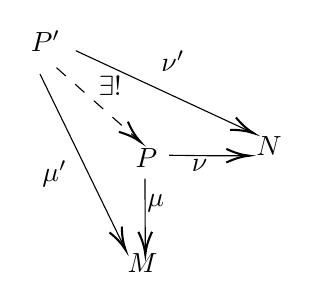
\begin{tikzpicture}[x=0.75pt,y=0.75pt,yscale=-1,xscale=1]
%uncomment if require: \path (0,174); %set diagram left start at 0, and has height of 174

%Straight Lines [id:da14204189206076934] 
\draw    (306.77,85.78) -- (325.49,86) -- (343.31,86) ;
\draw [shift={(345.31,86)}, rotate = 180] [color={rgb, 255:red, 0; green, 0; blue, 0 }  ][line width=0.75]    (10.93,-3.29) .. controls (6.95,-1.4) and (3.31,-0.3) .. (0,0) .. controls (3.31,0.3) and (6.95,1.4) .. (10.93,3.29)   ;
%Straight Lines [id:da8235252283498069] 
\draw    (261.87,35.41) -- (345.71,74.33) ;
\draw [shift={(347.53,75.17)}, rotate = 204.9] [color={rgb, 255:red, 0; green, 0; blue, 0 }  ][line width=0.75]    (10.93,-3.29) .. controls (6.95,-1.4) and (3.31,-0.3) .. (0,0) .. controls (3.31,0.3) and (6.95,1.4) .. (10.93,3.29)   ;
%Straight Lines [id:da17475908774999116] 
\draw    (244.6,46.68) -- (284.96,129.58) ;
\draw [shift={(285.84,131.38)}, rotate = 244.04] [color={rgb, 255:red, 0; green, 0; blue, 0 }  ][line width=0.75]    (10.93,-3.29) .. controls (6.95,-1.4) and (3.31,-0.3) .. (0,0) .. controls (3.31,0.3) and (6.95,1.4) .. (10.93,3.29)   ;
%Straight Lines [id:da6934758258550564] 
\draw    (295.16,97.04) -- (295.34,131.61) ;
\draw [shift={(295.35,133.61)}, rotate = 269.71] [color={rgb, 255:red, 0; green, 0; blue, 0 }  ][line width=0.75]    (10.93,-3.29) .. controls (6.95,-1.4) and (3.31,-0.3) .. (0,0) .. controls (3.31,0.3) and (6.95,1.4) .. (10.93,3.29)   ;
%Straight Lines [id:da06155844542742672] 
\draw  [dash pattern={on 4.5pt off 4.5pt}]  (252.53,43.6) -- (291.47,77.98) ;
\draw [shift={(292.97,79.3)}, rotate = 221.44] [color={rgb, 255:red, 0; green, 0; blue, 0 }  ][line width=0.75]    (10.93,-3.29) .. controls (6.95,-1.4) and (3.31,-0.3) .. (0,0) .. controls (3.31,0.3) and (6.95,1.4) .. (10.93,3.29)   ;

% Text Node
\draw (271.7,46.47) node [anchor=north west][inner sep=0.75pt]  [rotate=-359.79,xslant=0.02]  {$\exists !$};
% Text Node
\draw (244.48,87.07) node [anchor=north west][inner sep=0.75pt]    {$\mu ^{\prime }$};
% Text Node
\draw (301.79,34.25) node [anchor=north west][inner sep=0.75pt]    {$\nu ^{\prime }$};
% Text Node
\draw (295.06,103.69) node [anchor=north west][inner sep=0.75pt]    {$\mu $};
% Text Node
\draw (316.47,86.47) node [anchor=north west][inner sep=0.75pt]    {$\nu $};
% Text Node
\draw (238.93,24.58) node [anchor=north west][inner sep=0.75pt]    {$P^{\prime }$};
% Text Node
\draw (289.35,81.38) node [anchor=north west][inner sep=0.75pt]    {$P$};
% Text Node
\draw (285.56,131.96) node [anchor=north west][inner sep=0.75pt]    {$M$};
% Text Node
\draw (347.56,75.76) node [anchor=north west][inner sep=0.75pt]    {$N$};


\end{tikzpicture}
\end{center}
\\
\textbf{product} : a product is a diagram
\begin{center}
\tikzset{every picture/.style={line width=0.75pt}} %set default line width to 0.75pt        

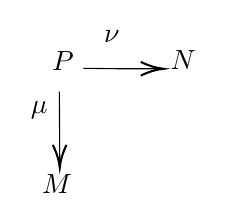
\begin{tikzpicture}[x=0.75pt,y=0.75pt,yscale=-1,xscale=1]
%uncomment if require: \path (0,131); %set diagram left start at 0, and has height of 131

%Straight Lines [id:da14204189206076934] 
\draw    (296.77,43.78) -- (315.49,44) -- (333.31,44) ;
\draw [shift={(335.31,44)}, rotate = 180] [color={rgb, 255:red, 0; green, 0; blue, 0 }  ][line width=0.75]    (10.93,-3.29) .. controls (6.95,-1.4) and (3.31,-0.3) .. (0,0) .. controls (3.31,0.3) and (6.95,1.4) .. (10.93,3.29)   ;
%Straight Lines [id:da6934758258550564] 
\draw    (285.16,55.04) -- (285.34,89.61) ;
\draw [shift={(285.35,91.61)}, rotate = 269.71] [color={rgb, 255:red, 0; green, 0; blue, 0 }  ][line width=0.75]    (10.93,-3.29) .. controls (6.95,-1.4) and (3.31,-0.3) .. (0,0) .. controls (3.31,0.3) and (6.95,1.4) .. (10.93,3.29)   ;

% Text Node
\draw (270.16,58.44) node [anchor=north west][inner sep=0.75pt]    {$\mu $};
% Text Node
\draw (305.47,24.47) node [anchor=north west][inner sep=0.75pt]    {$\nu $};
% Text Node
\draw (280.35,34.38) node [anchor=north west][inner sep=0.75pt]    {$P$};
% Text Node
\draw (275.56,93.96) node [anchor=north west][inner sep=0.75pt]    {$M$};
% Text Node
\draw (337.56,33.76) node [anchor=north west][inner sep=0.75pt]    {$N$};


\end{tikzpicture}
\end{center}
\\
\textbf{category $\mathscr C$} : a category consists of a collection of \textbf{objects}, and for each pair of objects, a set of \textbf{morphisms} (or \textbf{arrows}) between them

Morphisms are often informally called \textbf{maps}

\textbf{obj($\mathscr C$)} : The collection of objects of a category $\mathscr C$ is often denoted obj($\mathscr C$), but we will usually denote the collection also by $\mathscr C$

$\boldsymbol{Mor(A,B)}$ : If $A, B \in \mathscr C$ , then the set of morphisms from $A$ to $B$ is denoted $Mor(A, B)$

A morphism is often written $f : A \rightarrow B$, and $A$ is said to be the \textbf{source} of $f$, and $B$ the \textbf{target} of $f$

$Mor(B, C)\times Mor(A, B)\rightarrow Mor(A, C)$, and if $f \in Mor(A, B)$ and $g \in Mor(B, C)$, then their composition is denoted $g \circ f$. Composition is associative: if $f \in Mor(A, B), g \in Mor(B, C)$, and $h \in Mor(C, D)$, then $h \circ (g \circ f) = (h \circ g) \circ f$

\textbf{identity morphism} : For each object $A \in \mathscr C$ , there is always an identity morphism $id_A : A \rightarrow A$, such that when you (left- or right-)compose a morphism with the identity, you get the same morphism. More precisely, for any morphisms $f : A \rightarrow B$ and $g: B \rightarrow C$, $id_B \circ f = f$ and $g \circ id_B = g$

\textbf{isomorphism} : a notion of isomorphism between two objects of a category (a morphism $f : A \rightarrow B$ such that there exists some — necessarily unique — morphism $g: B \rightarrow A$, where $f \circ g$ and $g \circ f$ are the identity on $B$ and $A$ respectively)

\textbf{automorphism} : an isomorphism of the object with itself
\begin{example}
the category of sets, denoted $\boldsymbol{Sets}$. The objects are sets, and the morphisms are maps of sets
\label{1.1}
\end{example}
\begin{example}
the category $\boldsymbol{Vec_k}$ of vector spaces over a given field $k$. The objects are $k$-vector spaces, and the morphisms are linear transformations
\label{1.2}
\end{example}
\begin{example}
A category in which each morphism is an isomorphism is called a \textbf{groupoid}\\
(a) A perverse definition of a group is: a groupoid with one object. Make sense of this\\
(b) Describe a groupoid that is not a group
\end{example}
\textbf{automorphism group} : If $A$ is an object in a category $\mathscr C$ , then the invertible elements of $Mor(A, A)$ form a group (called the automorphism group of $A$, denoted $\boldsymbol{Aut(A)}$)

the automorphism groups of the objects in 

Example \ref{1.1} : $\left\{bijections\; between\; A\right\}$  

Example \ref{1.2} : $\left\{linear\; isomorphism\; on\; A\right\}$

Two isomorphic objects have isomorphic automorphism groups, but these groups are not canonically isomorphic : if $X$ is a topological space, then the fundamental groupoid is the category where the objects are points of $X$, and the morphisms $x \rightarrow y$ are paths from $x$ to $y$, up to homotopy. Then the automorphism group of $x_0$ is the (pointed) fundamental group $\pi_1(X, x_0)$. In the case where $X$ is connected, and $\pi_1(X)$ is not abelian, this illustrates the fact that for a connected groupoid, $\left\{x\right\}$ and $\left\{y\right\}$ have isomorphic automorphism groups, but $\pi_1(X,x)$ and $\pi_1(X,y)$ are not canonically isomorphic
\begin{example}
abelian groups: The abelian groups, along with group homomorphisms, form a category \textbf{Ab}
\label{1.4}
\end{example}
\begin{example}
Modules over a ring. If $A$ is a ring, then the $A$-modules form a category $\boldsymbol{Mod_A}$

Taking $A = k$, we obtain Example \ref{1.2}; taking $A =\mathbb Z$, we obtain Example \ref{1.4}
\end{example}
\begin{example}
$rings$. There is a category $\boldsymbol{Rings}$, where the objects are rings, and the morphisms are maps of rings in the usual sense
\end{example}
\begin{example}
$topological\; spaces$. The topological spaces, along with continuous maps, form a category $\boldsymbol{Top}$. The isomorphisms are homeomorphisms.
\end{example}
\begin{example}
partially ordered sets. A \textbf{partially ordered set}, (or \textbf{poset}), is a set $S$ along with a binary relation $\geq$ on $S$ satisfying:

(i) $x \geq x$ (reflexivity)

(ii) $x \geq y$ and $y \geq z$ imply $x \geq z$ (transitivity)

(iii) if $x \geq y$ and $y \geq x$ then $x = y$ (antisymmetry)

A partially ordered set $(S, \geq)$ can be interpreted as a category whose objects are the elements of $S$, and with a single morphism from $x$ to $y$ if and only if $x \geq y$ (and no morphism otherwise).
\end{example}
\begin{example}
the category of subsets of a set, and the category of open subsets of a topological space. If X is a set, then the subsets form a partially ordered set, where the order is given by inclusion. Informally, if $U \subset V$, then we have exactly one morphism $U \rightarrow V$ in the category (and otherwise none). Similarly, if X is a topological space, then the open sets form a partially ordered set, where the order is given by inclusion.
\end{example}
\textbf{subcategory} : a subcategory $\mathscr A$ of a category $\mathscr B$ has as its objects some of the objects of $\mathscr B$, and some of the morphisms, such that the morphisms of $\mathscr A$ include the identity morphisms of the objects of $\mathscr A$ , and are closed under composition
\\

\textbf{covariant functor} : a covariant functor $F$ from a category $\mathscr A$ to a category $\mathscr B$, denoted $F: \mathscr A \rightarrow \mathscr B$,
is the following data. It is a map of objects $F: obj(\mathscr A ) \rightarrow obj(\mathscr B)$, and for each $A_1, A_2 \in A$ , and morphism $m: A_1 \rightarrow A_2$, a morphism $F(m) : F(A_1) \rightarrow F(A_2)$ in $\mathscr B$

We require that $F$ preserves identity morphisms (for $A \in\mathscr A , F(id_A) = id_{F(A)}$), and that $F$ preserves composition $(F(m_2 \circ m_1) = F(m_2) \circ F(m_1))$

A trivial example is the \textbf{identity functor} $id:\mathscr A \rightarrow\mathscr A$\\

\textbf{forgetful functor} : Consider the functor from the category of
vector spaces (over a field $k$) $Vec_k$ to $Sets$, that associates to each vector space its underlying set. The functor sends a linear transformation to its underlying map of sets. This is an example of a forgetful functor, where some additional structure is forgotten

Another example of a forgetful functor is $Mod_A \rightarrow Ab$ from $A$-modules to abelian groups, remembering only the abelian group structure of the $A$-module
\begin{example}
Topological examples. (Examples of covariant functors)

fundamental group functor $\boldsymbol{\pi_1}$, which sends a topological space X with choice of a point $x_0 \in X$ to a group $\pi_1(X, x_0)$

The ith homology functor $\boldsymbol{Top \rightarrow Ab}$, which sends a topological space X to its ith homology group $H_i(X,\mathbb Z)$

The covariance corresponds to the fact that a (continuous) morphism of pointed topological spaces $\phi: X \rightarrow Y$ with $\phi(x_0) = y_0$ induces a map of fundamental groups $\pi_1(X, x_0) \rightarrow \pi_1(Y, y_0)$, and similarly for homology groups
\label{1.10}
\end{example}
\begin{example}
Suppose A is an object in a category $\mathscr C$. Then there is a functor $\boldsymbol{h^A :\mathscr C \rightarrow Sets}$ sending $B \in \mathscr C$ to $Mor(A, B)$, and sending $f : B_1 \rightarrow B_2$ to $Mor(A, B_1) \rightarrow Mor(A, B_2)$ described by
\begin{center}
$[g: A \rightarrow B_1] \mapsto[f \circ g: A \rightarrow B_1 \rightarrow B_2]$
\end{center}
\label{1.11}
\end{example}
\textbf{composition} : If $F: \mathscr A \rightarrow \mathscr B$ and $G: \mathscr B \rightarrow \mathscr C$ are covariant functors, then we
define a functor $G\circ F: \mathscr A \rightarrow \mathscr C$ (the composition of $G$ and $F$) in the obvious way\\

A covariant functor $F: \mathscr A \rightarrow \mathscr B$ is \textbf{faithful} if for all $A, A^\prime \in \mathscr A$, the map $Mor_{\mathscr A} (A, A^\prime) \rightarrow Mor_{\mathscr B}(F(A), F(A^\prime))$ is injective, and \textbf{full} if it is surjective. A functor that is full and faithful is \textbf{fully faithful}

A subcategory $i:\mathscr A \rightarrow \mathscr B$ is a full subcategory if $i$ is full. (Inclusions are always faithful, so there is no need for the phrase “faithful subcategory”.) Thus a subcategory $\mathscr A^\prime$ of $\mathscr A$ is full if and only if for all $A, B \in obj(\mathscr A^\prime)$, $ Mor_{\mathscr A^\prime} (A, B) = Mor_{\mathscr A}(A, B)$
\begin{example}
    the forgetful functor $Vec_k \rightarrow Sets$ is faithful, but not full; and if $A$ is a ring, the category of finitely generated $A$-modules is a full subcategory of the category $Mod_A$ of $A$-modules
\end{example}
\textbf{contravariant functor} : A contravariant functor is defined in the same way as a covariant functor, except the arrows switch directions: in the above language, $F(A_1 \rightarrow A_2)$ is now an arrow from $F(A_2)$ to $F(A_1)$. (Thus $F(m_2 \circ m_1) = F(m_1) \circ F(m_2)$, not
$F(m_2) \circ F(m_1)$.)

It is wise to state whether a functor is covariant or contravariant, unless the context makes it very clear. If it is not stated (and the context does not make it
clear), the functor is often assumed to be covariant\\

\textbf{opposite category} : $\mathscr C^{opp}$ is the same category as $\mathscr C$ except that the arrows go in the opposite direction. Here $\mathscr C^{opp}$ is said to be the opposite category to $\mathscr C$

Sometimes people describe a contravariant functor $\mathscr C \rightarrow \mathscr D$ as a covariant functor $\mathscr C^{opp} \rightarrow \mathscr D$

\begin{example}
    Linear algebra example \ref{1.2}
    
    If $Vec_k$ is the category of $k$-vector spaces, then taking duals gives a contravariant functor $(·) ^\vee: Vec_k \rightarrow Vec_k$. Indeed, to each linear transformation $f : V \rightarrow W$, we have a dual transformation $f^\vee : W^\vee \rightarrow V^\vee$, and $(f \circ g)^\vee = g^\vee \circ f^\vee$
    \label{1.13}
\end{example}
\begin{example}
    Topological example \ref{1.10}
    
    The $i$th cohomology functor $H_i(\cdot, \mathbb Z) : Top \rightarrow Ab$ is a contravariant functor
\end{example}
\begin{example}
    There is a contravariant functor $Top \rightarrow Rings$ taking a topological space $X$ to the ring of real-valued continuous functions on $X$. A morphism of topological spaces $X \rightarrow Y$ (a continuous map) induces the pullback map from functions on $Y$ to functions on $X$
    \label{1.15}
\end{example}
\begin{example}
     the \textbf{functor of points} \ref{1.11}
     
     Suppose $A$ is an object of a category $\mathscr C$. Then there is a contravariant functor $h_A : \mathscr C \rightarrow Sets$ sending $B \in \mathscr C$ to $Mor(B, A)$, and sending the morphism $f : B_1 \rightarrow B_2$ to the morphism $Mor(B_2, A) \rightarrow Mor(B_1, A)$ via
     \begin{center}
         $[g: B_2 \rightarrow A] \mapsto [g \circ f : B_1 \rightarrow B_2 \rightarrow A]$
     \end{center}
\end{example}
 Examples \ref{1.13} and \ref{1.15} may be interpreted as special cases\\

\textbf{natural transformation of covariant functors $F \rightarrow G$} : Suppose $F$ and $G$ are two covariant functors from $\mathscr A$ to $\mathscr B$. A natural transformation of covariant functors $F \rightarrow G$ is the data of a morphism $\mathfrak m_A : F(A) \rightarrow G(A)$ for each $A \in\mathscr A$ such that for each $f : A \rightarrow A^\prime$ in $\mathscr A$ , the diagram commutes:
\begin{center}
    \tikzset{every picture/.style={line width=0.75pt}} %set default line width to 0.75pt        

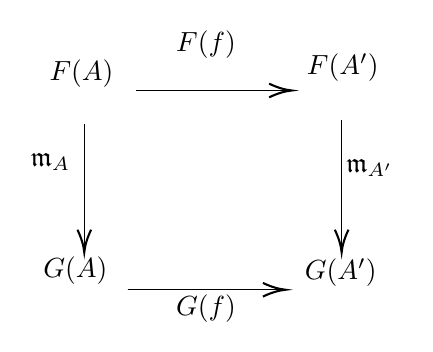
\begin{tikzpicture}[x=0.75pt,y=0.75pt,yscale=-1,xscale=1]
%uncomment if require: \path (0,182); %set diagram left start at 0, and has height of 182

%Straight Lines [id:da14204189206076934] 
\draw    (285,40) -- (315.49,40) -- (358,40) ;
\draw [shift={(360,40)}, rotate = 180] [color={rgb, 255:red, 0; green, 0; blue, 0 }  ][line width=0.75]    (10.93,-3.29) .. controls (6.95,-1.4) and (3.31,-0.3) .. (0,0) .. controls (3.31,0.3) and (6.95,1.4) .. (10.93,3.29)   ;
%Straight Lines [id:da6934758258550564] 
\draw    (260,56) -- (260,116) ;
\draw [shift={(260,118)}, rotate = 270] [color={rgb, 255:red, 0; green, 0; blue, 0 }  ][line width=0.75]    (10.93,-3.29) .. controls (6.95,-1.4) and (3.31,-0.3) .. (0,0) .. controls (3.31,0.3) and (6.95,1.4) .. (10.93,3.29)   ;
%Straight Lines [id:da5132351330329095] 
\draw    (289,136) -- (281,136) -- (355,136) ;
\draw [shift={(357,136)}, rotate = 180] [color={rgb, 255:red, 0; green, 0; blue, 0 }  ][line width=0.75]    (10.93,-3.29) .. controls (6.95,-1.4) and (3.31,-0.3) .. (0,0) .. controls (3.31,0.3) and (6.95,1.4) .. (10.93,3.29)   ;
%Straight Lines [id:da817882018823904] 
\draw    (384,54) -- (384,116) ;
\draw [shift={(384,118)}, rotate = 270] [color={rgb, 255:red, 0; green, 0; blue, 0 }  ][line width=0.75]    (10.93,-3.29) .. controls (6.95,-1.4) and (3.31,-0.3) .. (0,0) .. controls (3.31,0.3) and (6.95,1.4) .. (10.93,3.29)   ;

% Text Node
\draw (233,69) node [anchor=north west][inner sep=0.75pt]   [align=left] {
$\mathfrak{m}_{A}$
};
% Text Node
\draw (385,72) node [anchor=north west][inner sep=0.75pt]   [align=left] {
$\mathfrak{m}_{A^{\prime }}$
};
% Text Node
\draw (366,21) node [anchor=north west][inner sep=0.75pt]   [align=left] {
$F(A^{\prime } )$
};
% Text Node
\draw (365,120) node [anchor=north west][inner sep=0.75pt]   [align=left] {
$G(A^{\prime } )$
};
% Text Node
\draw (239,119) node [anchor=north west][inner sep=0.75pt]   [align=left] {
$G(A)$
};
% Text Node
\draw (242,24) node [anchor=north west][inner sep=0.75pt]   [align=left] {
$F(A)$
};
% Text Node
\draw (303,10) node [anchor=north west][inner sep=0.75pt]   [align=left] {
$F(f)$
};
% Text Node
\draw (303,137) node [anchor=north west][inner sep=0.75pt]   [align=left] {
$G(f)$
};


\end{tikzpicture}


\end{center}

\textbf{natural isomorphism} : A natural isomorphism of functors is a natural transformation such that each $m_A$ is an isomorphism. (We make analogous definitions when F and G are both contravariant.)

\textbf{equivalence of categories} : The data of functors $F: \mathscr A \rightarrow \mathscr B$ and $F^\prime: \mathscr B \rightarrow \mathscr A$ such that $F \circ F^\prime$ is naturally isomorphic to the identity functor $id_\mathscr B$ on $\mathscr B$ and $F^\prime \circ F$ is naturally isomorphic to $id_\mathscr A$ is said to be an equivalence of categories
\begin{example}
    Let $f.d.Vec_k$ be the category of finite-dimensional vector spaces over $k$
    
    Let $(\cdot)^{\vee\vee} : f.d.Vec_k \rightarrow f.d.Vec_k$ be the double dual functor from the category of finite-dimensional vector spaces over $k$ to itself. Then $(\cdot)^{\vee\vee}$ is naturally isomorphic to the identity functor on $f.d.Vec_k$. (Without the finite-dimensionality hypothesis, we only get a natural transformation of functors from $id$ to $(\cdot)^{\vee\vee}$)
\end{example}
Let $\mathscr V$ be the category whose objects are the $k$-vector spaces $k^n$ for each $n \geq 0$ (there is one vector space for each $n$), and whose morphisms are linear transformations. The objects of $\mathscr V$ can be thought of as vector spaces with bases, and the morphisms as matrices. There is an obvious functor $\mathscr V \rightarrow f.d.Vec_k$, as each $k^n$ is a
finite-dimensional vector space
\begin{example}
    $\mathscr V \rightarrow f.d.Vec_k$ gives an equivalence of categories, by describing an “inverse” functor
\end{example}





\newpage
\subsection{Universal properties determine an object up to unique isomorphism}

\textbf{Products were defined by a universal property}

\textbf{initial objects} : An object of a category $\mathscr C$ is an initial object if it has precisely one map to every object 

\textbf{final objects} : It is a final object if it has precisely one map from every object

\textbf{zero objects} : It is a zero object if it is both an initial object and a final object
\begin{example}
    Any two initial objects are uniquely isomorphic. Any two final objects are uniquely isomorphic
\end{example}
This (partially) justifies the phrase “the initial object”
rather than “an initial object”, and similarly for “the final object” and “the zero
object”

(Convention: we often say “the”, not “a”, for anything defined up to unique isomorphism)
\begin{example}
     The initial and final objects in Sets, Rings, and Top (if they exist)?
\end{example}
\textbf{Localization of rings and modules}

$A \rightarrow S^{-1}A$ satisfies the following universal property:

$S^{-1}A$ is initial among $A$-algebras $B$ where every element of $S$ is sent to an invertible element in B. (Recall: the data of “an $A$-algebra $B$” and “a ring map $A \rightarrow B$” are the same)

Translation: any map $A \rightarrow B$ where every element of $S$ is sent to an
invertible element must factor uniquely through $A \rightarrow S^{-1}A$

Another translation:
a ring map out of $S^{-1}A$ is the same thing as a ring map from $A$ that sends every
element of $S$ to an invertible element\\

\textbf{Category theoretic description} : If $A$ is a ring and $S$ is a subset, consider all $A$-algebras $B$, so that, under the canonical homomorphism $A\rightarrow B$, every element of $S$ is mapped to a unit. These algebras are the objects of a category, with $A$-algebra homomorphisms as morphisms. Then, the localization of $A$ at $S$ is the initial object of this category. (This is a more abstract way of expressing the universal property above.)\\


Furthermore, an $S^{-1}A$-module is the same thing as an $A$-module for which $s \times \cdot: M \rightarrow M$ is an $A$-module isomorphism for all $s \in S$

 Let’s get some practice with this by defining localizations of modules by universal property. Suppose M is an A-module. We define the A-module map
$\phi: M \rightarrow S^{-1}M$ as being initial among $A$-module maps $M \rightarrow N$ such that elements of $S$ are invertible in $N$ ($s \times \cdot: N \rightarrow N$ is an isomorphism for all $s \in S$). More precisely, any such map $\alpha: M \rightarrow N$ factors uniquely through $\phi$:



\tikzset{every picture/.style={line width=0.75pt}} %set default line width to 0.75pt        
\begin{center}
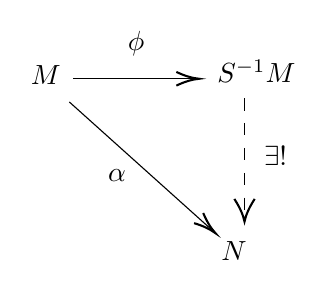
\begin{tikzpicture}[x=0.75pt,y=0.75pt,yscale=-1,xscale=1]
%uncomment if require: \path (0,140); %set diagram left start at 0, and has height of 140

%Straight Lines [id:da14204189206076934] 
\draw    (273.21,31.05) -- (291.45,31.05) -- (331.83,31.05) ;
\draw [shift={(333.83,31.05)}, rotate = 180] [color={rgb, 255:red, 0; green, 0; blue, 0 }  ][line width=0.75]    (10.93,-3.29) .. controls (6.95,-1.4) and (3.31,-0.3) .. (0,0) .. controls (3.31,0.3) and (6.95,1.4) .. (10.93,3.29)   ;
%Straight Lines [id:da6934758258550564] 
\draw    (271.31,42.21) -- (340.27,104.13) ;
\draw [shift={(341.76,105.47)}, rotate = 221.92] [color={rgb, 255:red, 0; green, 0; blue, 0 }  ][line width=0.75]    (10.93,-3.29) .. controls (6.95,-1.4) and (3.31,-0.3) .. (0,0) .. controls (3.31,0.3) and (6.95,1.4) .. (10.93,3.29)   ;
%Straight Lines [id:da817882018823904] 
\draw  [dash pattern={on 4.5pt off 4.5pt}]  (355.72,40.35) -- (355.72,97.88) ;
\draw [shift={(355.72,99.88)}, rotate = 270] [color={rgb, 255:red, 0; green, 0; blue, 0 }  ][line width=0.75]    (10.93,-4.9) .. controls (6.95,-2.3) and (3.31,-0.67) .. (0,0) .. controls (3.31,0.67) and (6.95,2.3) .. (10.93,4.9)   ;

% Text Node
\draw (251.52,23.45) node [anchor=north west][inner sep=0.75pt]    {$M$};
% Text Node
\draw (298.29,6.7) node [anchor=north west][inner sep=0.75pt]    {$\phi $};
% Text Node
\draw (341.39,20.62) node [anchor=north west][inner sep=0.75pt]    {$S^{-1} M$};
% Text Node
\draw (288.79,73.68) node [anchor=north west][inner sep=0.75pt]    {$\alpha $};
% Text Node
\draw (343.31,108.1) node [anchor=north west][inner sep=0.75pt]    {$N$};
% Text Node
\draw (363.88,62.52) node [anchor=north west][inner sep=0.75pt]    {$\exists !$};


\end{tikzpicture}
\end{center}

(Translation: $M \rightarrow S^{-1}M$ is universal (initial) among $A$-module maps from $M$ to modules that are actually $S^{-1}A$-modules)\\
\\
\textbf{Tensor products}

Another important example of a universal property construction is the notion of a tensor product of A-modules
\begin{align*}
\label{sup}
\otimes_A : obj(Mod_A) \times obj(Mod_A)
&\rightarrow
obj(Mod_A)
\\
(M, N)
&\rightarrow
M \otimes_A N
\end{align*}

\begin{proposition}
$ (\cdot)\otimes_A N$ gives a covariant functor $Mod_A \rightarrow Mod_A$. Then $(\cdot)\otimes_A N$ is a \textbf{right-exact} functor, i.e., if
$
M^\prime \rightarrow
M \rightarrow
M^{\prime\prime} \rightarrow
0
$
is an exact sequence of $A$-modules,  then the induced sequence is also exact:
$$
M^\prime\otimes_A N \rightarrow
M\otimes_A N \rightarrow
M^{\prime\prime}\otimes_A N \rightarrow
0
$$
\end{proposition}

\textbf{Category theoretic description} : a tensor product of $M$ and $N$ is an $A$-module $T$ along with an $A$-bilinear map $t : M \times N \rightarrow T$, such that given any $A$-bilinear map $t^\prime: M \times N \rightarrow T^\prime$
, there is a unique $A$-linear map $f : T \rightarrow T^\prime$ such
that $t^\prime = f \circ t$
\begin{center}
    

\tikzset{every picture/.style={line width=0.75pt}} %set default line width to 0.75pt        

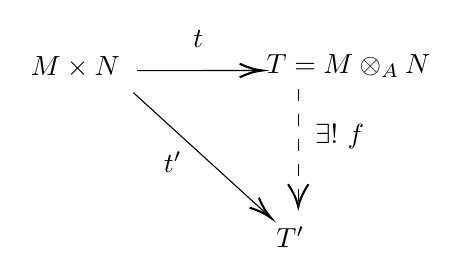
\begin{tikzpicture}[x=0.75pt,y=0.75pt,yscale=-1,xscale=1]
%uncomment if require: \path (0,128); %set diagram left start at 0, and has height of 128

%Straight Lines [id:da14204189206076934] 
\draw    (269.96,30.02) -- (287.12,30.02) -- (328.3,29.97) ;
\draw [shift={(330.3,29.97)}, rotate = 179.94] [color={rgb, 255:red, 0; green, 0; blue, 0 }  ][line width=0.75]    (10.93,-3.29) .. controls (6.95,-1.4) and (3.31,-0.3) .. (0,0) .. controls (3.31,0.3) and (6.95,1.4) .. (10.93,3.29)   ;
%Straight Lines [id:da6934758258550564] 
\draw    (268.17,40.67) -- (332.99,99.67) ;
\draw [shift={(334.47,101.01)}, rotate = 222.31] [color={rgb, 255:red, 0; green, 0; blue, 0 }  ][line width=0.75]    (10.93,-3.29) .. controls (6.95,-1.4) and (3.31,-0.3) .. (0,0) .. controls (3.31,0.3) and (6.95,1.4) .. (10.93,3.29)   ;
%Straight Lines [id:da817882018823904] 
\draw  [dash pattern={on 4.5pt off 4.5pt}]  (347.61,38.89) -- (347.61,93.69) ;
\draw [shift={(347.61,95.69)}, rotate = 270] [color={rgb, 255:red, 0; green, 0; blue, 0 }  ][line width=0.75]    (10.93,-4.9) .. controls (6.95,-2.3) and (3.31,-0.67) .. (0,0) .. controls (3.31,0.67) and (6.95,2.3) .. (10.93,4.9)   ;

% Text Node
\draw (335.85,103.88) node [anchor=north west][inner sep=0.75pt]    {$T^{\prime }$};
% Text Node
\draw (217.5,22.05) node [anchor=north west][inner sep=0.75pt]    {$M\times N$};
% Text Node
\draw (331.07,21.05) node [anchor=north west][inner sep=0.75pt]    {$T=M\otimes _{A} N$};
% Text Node
\draw (295.7,9.61) node [anchor=north west][inner sep=0.75pt]    {$t$};
% Text Node
\draw (281.64,67.82) node [anchor=north west][inner sep=0.75pt]    {$t^{\prime }$};
% Text Node
\draw (354.51,54.49) node [anchor=north west][inner sep=0.75pt]    {$\exists !\ f$};


\end{tikzpicture}
\end{center}
\begin{remark}
(a) If $M$ is an $A$-module and $A \rightarrow B$ is a morphism of rings, give $B \otimes_A M$ the structure of a $B$-module. This describes a functor
$Mod_A \rightarrow Mod_B$
\\
(b) If further $A \rightarrow C$ is another morphism of rings, show that $B \otimes_A C$ has a natural structure of a ring. Hint: multiplication will be given by 
$(b_1 \otimes c_1)(b_2 \otimes c_2) = (b_1b_2)\otimes(c_1c_2)$
\end{remark}
\begin{remark}
    If $S$ is a multiplicative subset of $A$ and $M$ is an $A$-module, there is a natural isomorphism $(S^{-1}A)\otimes_A M \cong S^{-1}M$ (as $S^{-1}A$-modules and as $A$-modules)
\end{remark}
\begin{remark}
     tensor products commute with arbitrary direct sums: if $M$ and $\left\{N_i\right\}_{i\in I}$ are all $A$-modules, describe an isomorphism
\begin{center}
    $M \otimes (\oplus_{i\in I}N_i)
\cong \oplus_{i\in I} (M \otimes N_i)$
\end{center}
\end{remark}

\textbf{Fibered products}

Suppose we have morphisms
$\alpha: X \rightarrow Z$ and $\beta: Y \rightarrow Z$ (in any category). Then the fibered product (or fibred product) is an object $X \times_Z Y$ along with morphisms $pr_X : X \times_Z Y \rightarrow X$ and
$pr_Y : X \times_Z Y \rightarrow Y$, where the two compositions $\alpha \circ pr_X$, $\beta \circ pr_Y : X \times_Z Y \rightarrow Z$ agree, such that given any object $W$ with maps to $X$ and $Y$ (whose compositions to $Z$ agree), these maps factor through some unique $W \rightarrow X \times_Z Y$:
\begin{center}


\tikzset{every picture/.style={line width=0.75pt}} %set default line width to 0.75pt        

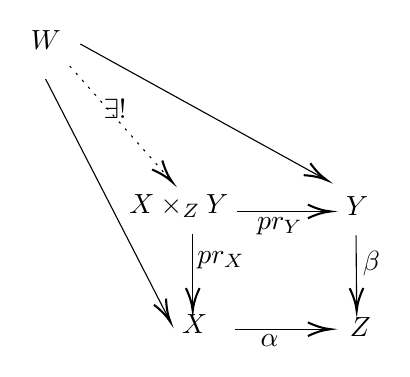
\begin{tikzpicture}[x=0.75pt,y=0.75pt,yscale=-1,xscale=1]
%uncomment if require: \path (0,179); %set diagram left start at 0, and has height of 179

%Straight Lines [id:da05850392395462478] 
\draw  [dash pattern={on 0.84pt off 2.51pt}]  (224.05,23.5) -- (272.09,77.85) ;
\draw [shift={(273.41,79.35)}, rotate = 228.53] [color={rgb, 255:red, 0; green, 0; blue, 0 }  ][line width=0.75]    (10.93,-3.29) .. controls (6.95,-1.4) and (3.31,-0.3) .. (0,0) .. controls (3.31,0.3) and (6.95,1.4) .. (10.93,3.29)   ;
%Straight Lines [id:da3774407613045476] 
\draw    (304.53,93.54) -- (347.71,93.54) ;
\draw [shift={(349.71,93.54)}, rotate = 180] [color={rgb, 255:red, 0; green, 0; blue, 0 }  ][line width=0.75]    (10.93,-3.29) .. controls (6.95,-1.4) and (3.31,-0.3) .. (0,0) .. controls (3.31,0.3) and (6.95,1.4) .. (10.93,3.29)   ;
%Straight Lines [id:da16928860805508283] 
\draw    (303.63,150.27) -- (347.71,150.27) ;
\draw [shift={(349.71,150.27)}, rotate = 180] [color={rgb, 255:red, 0; green, 0; blue, 0 }  ][line width=0.75]    (10.93,-3.29) .. controls (6.95,-1.4) and (3.31,-0.3) .. (0,0) .. controls (3.31,0.3) and (6.95,1.4) .. (10.93,3.29)   ;
%Straight Lines [id:da07214758061938187] 
\draw    (283.29,104.17) -- (283.29,139.41) ;
\draw [shift={(283.29,141.41)}, rotate = 270] [color={rgb, 255:red, 0; green, 0; blue, 0 }  ][line width=0.75]    (10.93,-3.29) .. controls (6.95,-1.4) and (3.31,-0.3) .. (0,0) .. controls (3.31,0.3) and (6.95,1.4) .. (10.93,3.29)   ;
%Straight Lines [id:da009828047720575217] 
\draw    (361.97,105.06) -- (362.25,139.41) ;
\draw [shift={(362.27,141.41)}, rotate = 269.53] [color={rgb, 255:red, 0; green, 0; blue, 0 }  ][line width=0.75]    (10.93,-3.29) .. controls (6.95,-1.4) and (3.31,-0.3) .. (0,0) .. controls (3.31,0.3) and (6.95,1.4) .. (10.93,3.29)   ;
%Straight Lines [id:da9760813772820314] 
\draw    (212.38,29.71) -- (271.6,144.95) ;
\draw [shift={(272.51,146.72)}, rotate = 242.8] [color={rgb, 255:red, 0; green, 0; blue, 0 }  ][line width=0.75]    (10.93,-3.29) .. controls (6.95,-1.4) and (3.31,-0.3) .. (0,0) .. controls (3.31,0.3) and (6.95,1.4) .. (10.93,3.29)   ;
%Straight Lines [id:da40981464659179734] 
\draw    (229.13,12.86) -- (346.16,77.5) ;
\draw [shift={(347.91,78.46)}, rotate = 208.91] [color={rgb, 255:red, 0; green, 0; blue, 0 }  ][line width=0.75]    (10.93,-3.29) .. controls (6.95,-1.4) and (3.31,-0.3) .. (0,0) .. controls (3.31,0.3) and (6.95,1.4) .. (10.93,3.29)   ;

% Text Node
\draw (251.55,84.05) node [anchor=north west][inner sep=0.75pt]    {$X\times _{Z} Y$};
% Text Node
\draw (276.88,141.78) node [anchor=north west][inner sep=0.75pt]    {$X$};
% Text Node
\draw (355.92,85.05) node [anchor=north west][inner sep=0.75pt]    {$Y$};
% Text Node
\draw (357.72,143.56) node [anchor=north west][inner sep=0.75pt]    {$Z$};
% Text Node
\draw (314.68,151.54) node [anchor=north west][inner sep=0.75pt]    {$\alpha $};
% Text Node
\draw (364.05,111.64) node [anchor=north west][inner sep=0.75pt]    {$\beta $};
% Text Node
\draw (284.3,111.53) node [anchor=north west][inner sep=0.75pt]    {$pr_{X}$};
% Text Node
\draw (313.07,95.03) node [anchor=north west][inner sep=0.75pt]    {$pr_{Y}$};
% Text Node
\draw (204.03,5.26) node [anchor=north west][inner sep=0.75pt]    {$W$};
% Text Node
\draw (239.03,38.06) node [anchor=north west][inner sep=0.75pt]    {$\exists !$};


\end{tikzpicture}
\end{center}
Depending on your religion, the diagram
\begin{center}
    

\tikzset{every picture/.style={line width=0.75pt}} %set default line width to 0.75pt        

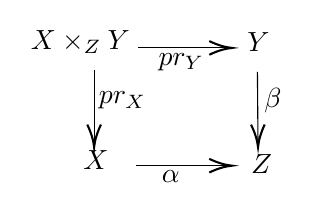
\begin{tikzpicture}[x=0.75pt,y=0.75pt,yscale=-1,xscale=1]
%uncomment if require: \path (0,96); %set diagram left start at 0, and has height of 96

%Straight Lines [id:da3774407613045476] 
\draw    (310.53,18.54) -- (353.71,18.54) ;
\draw [shift={(355.71,18.54)}, rotate = 180] [color={rgb, 255:red, 0; green, 0; blue, 0 }  ][line width=0.75]    (10.93,-3.29) .. controls (6.95,-1.4) and (3.31,-0.3) .. (0,0) .. controls (3.31,0.3) and (6.95,1.4) .. (10.93,3.29)   ;
%Straight Lines [id:da16928860805508283] 
\draw    (309.63,75.27) -- (353.71,75.27) ;
\draw [shift={(355.71,75.27)}, rotate = 180] [color={rgb, 255:red, 0; green, 0; blue, 0 }  ][line width=0.75]    (10.93,-3.29) .. controls (6.95,-1.4) and (3.31,-0.3) .. (0,0) .. controls (3.31,0.3) and (6.95,1.4) .. (10.93,3.29)   ;
%Straight Lines [id:da07214758061938187] 
\draw    (289.29,29.17) -- (289.29,64.41) ;
\draw [shift={(289.29,66.41)}, rotate = 270] [color={rgb, 255:red, 0; green, 0; blue, 0 }  ][line width=0.75]    (10.93,-3.29) .. controls (6.95,-1.4) and (3.31,-0.3) .. (0,0) .. controls (3.31,0.3) and (6.95,1.4) .. (10.93,3.29)   ;
%Straight Lines [id:da009828047720575217] 
\draw    (367.97,30.06) -- (368.25,64.41) ;
\draw [shift={(368.27,66.41)}, rotate = 269.53] [color={rgb, 255:red, 0; green, 0; blue, 0 }  ][line width=0.75]    (10.93,-3.29) .. controls (6.95,-1.4) and (3.31,-0.3) .. (0,0) .. controls (3.31,0.3) and (6.95,1.4) .. (10.93,3.29)   ;

% Text Node
\draw (257.55,9.05) node [anchor=north west][inner sep=0.75pt]    {$X\times _{Z} Y$};
% Text Node
\draw (282.88,66.78) node [anchor=north west][inner sep=0.75pt]    {$X$};
% Text Node
\draw (361.92,10.05) node [anchor=north west][inner sep=0.75pt]    {$Y$};
% Text Node
\draw (363.72,68.56) node [anchor=north west][inner sep=0.75pt]    {$Z$};
% Text Node
\draw (320.68,76.54) node [anchor=north west][inner sep=0.75pt]    {$\alpha $};
% Text Node
\draw (370.05,36.64) node [anchor=north west][inner sep=0.75pt]    {$\beta $};
% Text Node
\draw (290.3,38.53) node [anchor=north west][inner sep=0.75pt]    {$pr_{X}$};
% Text Node
\draw (319.07,20.03) node [anchor=north west][inner sep=0.75pt]    {$pr_{Y}$};


\end{tikzpicture}
\end{center}
is called a \textbf{fibered/pullback/Cartesian diagram/square} (six possibilities — even
more are possible if you prefer “fibred” to “fibered”)


\begin{example}
    In $Sets$,
$X \times_Z Y = \left\{(x, y) \in X \times Y : \alpha(x) = \beta(y)\right\}$.
\end{example}
\begin{example}
    If $Z$ is the final object in a category $\mathscr C$ , and $X, Y \in\mathscr C$ , then $X \times_Z Y = X \times Y$ : “the” fibered product over $Z$ is uniquely isomorphic to “the” product. (Assume all relevant (fibered) products exist)
\end{example}
\begin{example}
    If the two squares in the following commutative diagram are Cartesian diagrams, show that the “outside rectangle” (involving $U, V, Y,$ and $Z$) is also a Cartesian diagram
    \begin{center}
        

\tikzset{every picture/.style={line width=0.75pt}} %set default line width to 0.75pt        

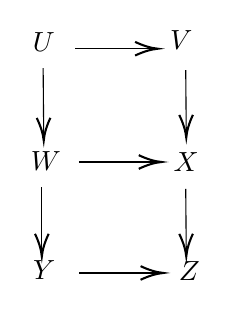
\begin{tikzpicture}[x=0.75pt,y=0.75pt,yscale=-1,xscale=1]
%uncomment if require: \path (0,139); %set diagram left start at 0, and has height of 139

%Straight Lines [id:da3774407613045476] 
\draw    (292.25,67.8) -- (330.06,67.8) ;
\draw [shift={(332.06,67.8)}, rotate = 180] [color={rgb, 255:red, 0; green, 0; blue, 0 }  ][line width=0.75]    (10.93,-3.29) .. controls (6.95,-1.4) and (3.31,-0.3) .. (0,0) .. controls (3.31,0.3) and (6.95,1.4) .. (10.93,3.29)   ;
%Straight Lines [id:da16928860805508283] 
\draw    (292.34,121.26) -- (330.94,121.26) ;
\draw [shift={(332.94,121.26)}, rotate = 180] [color={rgb, 255:red, 0; green, 0; blue, 0 }  ][line width=0.75]    (10.93,-3.29) .. controls (6.95,-1.4) and (3.31,-0.3) .. (0,0) .. controls (3.31,0.3) and (6.95,1.4) .. (10.93,3.29)   ;
%Straight Lines [id:da07214758061938187] 
\draw    (274.42,80.01) -- (274.42,111.33) ;
\draw [shift={(274.42,113.33)}, rotate = 270] [color={rgb, 255:red, 0; green, 0; blue, 0 }  ][line width=0.75]    (10.93,-3.29) .. controls (6.95,-1.4) and (3.31,-0.3) .. (0,0) .. controls (3.31,0.3) and (6.95,1.4) .. (10.93,3.29)   ;
%Straight Lines [id:da009828047720575217] 
\draw    (343.75,80.8) -- (344,111.33) ;
\draw [shift={(344.01,113.33)}, rotate = 269.54] [color={rgb, 255:red, 0; green, 0; blue, 0 }  ][line width=0.75]    (10.93,-3.29) .. controls (6.95,-1.4) and (3.31,-0.3) .. (0,0) .. controls (3.31,0.3) and (6.95,1.4) .. (10.93,3.29)   ;
%Straight Lines [id:da712845763467731] 
\draw    (275.05,22.58) -- (275.33,55.48) ;
\draw [shift={(275.34,57.48)}, rotate = 269.52] [color={rgb, 255:red, 0; green, 0; blue, 0 }  ][line width=0.75]    (10.93,-3.29) .. controls (6.95,-1.4) and (3.31,-0.3) .. (0,0) .. controls (3.31,0.3) and (6.95,1.4) .. (10.93,3.29)   ;
%Straight Lines [id:da0762263378097261] 
\draw    (343.75,23.53) -- (344,54.05) ;
\draw [shift={(344.01,56.05)}, rotate = 269.54] [color={rgb, 255:red, 0; green, 0; blue, 0 }  ][line width=0.75]    (10.93,-3.29) .. controls (6.95,-1.4) and (3.31,-0.3) .. (0,0) .. controls (3.31,0.3) and (6.95,1.4) .. (10.93,3.29)   ;
%Straight Lines [id:da6755292210517136] 
\draw    (290.49,13.22) -- (328.3,13.22) ;
\draw [shift={(330.3,13.22)}, rotate = 180] [color={rgb, 255:red, 0; green, 0; blue, 0 }  ][line width=0.75]    (10.93,-3.29) .. controls (6.95,-1.4) and (3.31,-0.3) .. (0,0) .. controls (3.31,0.3) and (6.95,1.4) .. (10.93,3.29)   ;

% Text Node
\draw (336.67,61.86) node [anchor=north west][inner sep=0.75pt]    {$X$};
% Text Node
\draw (268.92,114) node [anchor=north west][inner sep=0.75pt]    {$Y$};
% Text Node
\draw (339.23,114.45) node [anchor=north west][inner sep=0.75pt]    {$Z$};
% Text Node
\draw (267.87,61.51) node [anchor=north west][inner sep=0.75pt]    {$W$};
% Text Node
\draw (268.87,4.24) node [anchor=north west][inner sep=0.75pt]    {$U$};
% Text Node
\draw (335.01,3.35) node [anchor=north west][inner sep=0.75pt]    {$V$};


\end{tikzpicture}
    \end{center}
\end{example}
\begin{example}
    Given morphisms $X_1 \rightarrow Y, X_2 \rightarrow Y$, and $Y \rightarrow Z$, then there is a natural morphism $X_1 \times_Y X_2 \rightarrow X_1 \times_Z X_2$
\end{example}
\begin{remark}
    \textbf{The magic diagram}
    
    Suppose we are given morphisms $X_1, X_2 \rightarrow Y$ and $Y \rightarrow Z$. Then the following diagram is a Cartesian square :
    \begin{center}


\tikzset{every picture/.style={line width=0.75pt}} %set default line width to 0.75pt        

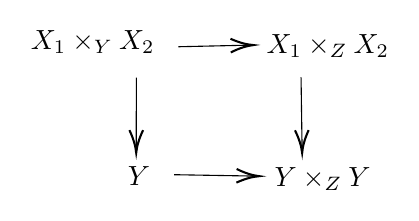
\begin{tikzpicture}[x=0.75pt,y=0.75pt,yscale=-1,xscale=1]
%uncomment if require: \path (0,97); %set diagram left start at 0, and has height of 97

%Straight Lines [id:da3774407613045476] 
\draw    (286.25,12.8) -- (320.33,12.04) ;
\draw [shift={(322.33,12)}, rotate = 178.72] [color={rgb, 255:red, 0; green, 0; blue, 0 }  ][line width=0.75]    (10.93,-3.29) .. controls (6.95,-1.4) and (3.31,-0.3) .. (0,0) .. controls (3.31,0.3) and (6.95,1.4) .. (10.93,3.29)   ;
%Straight Lines [id:da16928860805508283] 
\draw    (284.14,74.45) -- (323.16,75.12) ;
\draw [shift={(325.16,75.16)}, rotate = 180.99] [color={rgb, 255:red, 0; green, 0; blue, 0 }  ][line width=0.75]    (10.93,-3.29) .. controls (6.95,-1.4) and (3.31,-0.3) .. (0,0) .. controls (3.31,0.3) and (6.95,1.4) .. (10.93,3.29)   ;
%Straight Lines [id:da07214758061938187] 
\draw    (265.97,27.73) -- (265.9,61.92) ;
\draw [shift={(265.89,63.92)}, rotate = 270.12] [color={rgb, 255:red, 0; green, 0; blue, 0 }  ][line width=0.75]    (10.93,-3.29) .. controls (6.95,-1.4) and (3.31,-0.3) .. (0,0) .. controls (3.31,0.3) and (6.95,1.4) .. (10.93,3.29)   ;
%Straight Lines [id:da009828047720575217] 
\draw    (345.31,27.58) -- (345.81,61.96) ;
\draw [shift={(345.84,63.96)}, rotate = 269.16] [color={rgb, 255:red, 0; green, 0; blue, 0 }  ][line width=0.75]    (10.93,-3.29) .. controls (6.95,-1.4) and (3.31,-0.3) .. (0,0) .. controls (3.31,0.3) and (6.95,1.4) .. (10.93,3.29)   ;

% Text Node
\draw (260.56,69.27) node [anchor=north west][inner sep=0.75pt]    {$Y$};
% Text Node
\draw (331.3,69.92) node [anchor=north west][inner sep=0.75pt]    {$Y\times _{Z} Y$};
% Text Node
\draw (213.87,3.88) node [anchor=north west][inner sep=0.75pt]    {$X_{1} \times _{Y} X_{2}$};
% Text Node
\draw (327.46,5.83) node [anchor=north west][inner sep=0.75pt]    {$X_{1} \times _{Z} X_{2}$};


\end{tikzpicture}
    \end{center}
    (Assume all relevant (fibered) products exist)
    
    (Hint : if $Y\times_Z Y$ exists, then 
    $X_1\times_Z X_2 \rightarrow X_2 \rightarrow Y$ and
    $X_1\times_Z X_2 \rightarrow X_1 \rightarrow Y$
    are equal)
\end{remark}

\textbf{Coproducts}

Define coproduct in a category by reversing all the arrows in
the definition of product. 

For $\mathscr C$ a category and ,$X,Y\in Obj(\mathscr C)$
 two objects, their coproduct is an object $X\amalg Y$ in $\mathscr C$ equipped with two morphisms
\begin{center}
    

\tikzset{every picture/.style={line width=0.75pt}} %set default line width to 0.75pt        

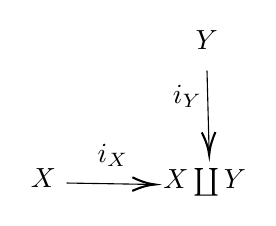
\begin{tikzpicture}[x=0.75pt,y=0.75pt,yscale=-1,xscale=1]
%uncomment if require: \path (0,94); %set diagram left start at 0, and has height of 94

%Straight Lines [id:da16928860805508283] 
\draw    (199.85,77.91) -- (240.39,78.58) ;
\draw [shift={(242.39,78.62)}, rotate = 180.96] [color={rgb, 255:red, 0; green, 0; blue, 0 }  ][line width=0.75]    (10.93,-3.29) .. controls (6.95,-1.4) and (3.31,-0.3) .. (0,0) .. controls (3.31,0.3) and (6.95,1.4) .. (10.93,3.29)   ;
%Straight Lines [id:da009828047720575217] 
\draw    (267.43,23.71) -- (268.44,62.38) ;
\draw [shift={(268.49,64.38)}, rotate = 268.5] [color={rgb, 255:red, 0; green, 0; blue, 0 }  ][line width=0.75]    (10.93,-3.29) .. controls (6.95,-1.4) and (3.31,-0.3) .. (0,0) .. controls (3.31,0.3) and (6.95,1.4) .. (10.93,3.29)   ;

% Text Node
\draw (260.67,3.33) node [anchor=north west][inner sep=0.75pt]    {$Y$};
% Text Node
\draw (181.3,69.52) node [anchor=north west][inner sep=0.75pt]    {$X$};
% Text Node
\draw (245.15,69.52) node [anchor=north west][inner sep=0.75pt]    {$X\coprod Y$};
% Text Node
\draw (213.48,57.79) node [anchor=north west][inner sep=0.75pt]    {$i_{X}$};
% Text Node
\draw (249.78,29.62) node [anchor=north west][inner sep=0.75pt]    {$i_{Y}$};


\end{tikzpicture}
\end{center}
such that this is universal with this property, meaning such that for any other object with maps like this
\begin{center}
    

\tikzset{every picture/.style={line width=0.75pt}} %set default line width to 0.75pt        

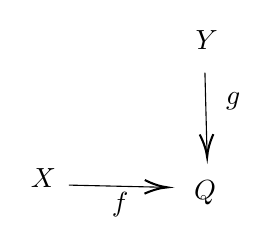
\begin{tikzpicture}[x=0.75pt,y=0.75pt,yscale=-1,xscale=1]
%uncomment if require: \path (0,107); %set diagram left start at 0, and has height of 107

%Straight Lines [id:da16928860805508283] 
\draw    (200.85,78.91) -- (246.33,79.95) ;
\draw [shift={(248.33,80)}, rotate = 181.32] [color={rgb, 255:red, 0; green, 0; blue, 0 }  ][line width=0.75]    (10.93,-3.29) .. controls (6.95,-1.4) and (3.31,-0.3) .. (0,0) .. controls (3.31,0.3) and (6.95,1.4) .. (10.93,3.29)   ;
%Straight Lines [id:da009828047720575217] 
\draw    (266.43,24.71) -- (267.44,63.38) ;
\draw [shift={(267.49,65.38)}, rotate = 268.5] [color={rgb, 255:red, 0; green, 0; blue, 0 }  ][line width=0.75]    (10.93,-3.29) .. controls (6.95,-1.4) and (3.31,-0.3) .. (0,0) .. controls (3.31,0.3) and (6.95,1.4) .. (10.93,3.29)   ;

% Text Node
\draw (260.67,3.33) node [anchor=north west][inner sep=0.75pt]    {$Y$};
% Text Node
\draw (181.3,69.52) node [anchor=north west][inner sep=0.75pt]    {$X$};
% Text Node
\draw (260.02,75.34) node [anchor=north west][inner sep=0.75pt]    {$Q$};
% Text Node
\draw (220.3,81.13) node [anchor=north west][inner sep=0.75pt]    {$f$};
% Text Node
\draw (275.43,33.11) node [anchor=north west][inner sep=0.75pt]    {$g$};


\end{tikzpicture}
\end{center}
there exists a unique morphism $(f,g) : X\coprod Y \rightarrow Q$ such that we have the following commuting diagram:
\begin{center}
    

\tikzset{every picture/.style={line width=0.75pt}} %set default line width to 0.75pt        

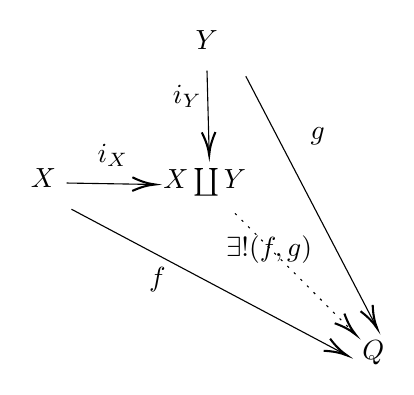
\begin{tikzpicture}[x=0.75pt,y=0.75pt,yscale=-1,xscale=1]
%uncomment if require: \path (0,176); %set diagram left start at 0, and has height of 176

%Straight Lines [id:da3774407613045476] 
\draw    (286.13,26.46) -- (348.46,146.1) ;
\draw [shift={(349.38,147.87)}, rotate = 242.48] [color={rgb, 255:red, 0; green, 0; blue, 0 }  ][line width=0.75]    (10.93,-3.29) .. controls (6.95,-1.4) and (3.31,-0.3) .. (0,0) .. controls (3.31,0.3) and (6.95,1.4) .. (10.93,3.29)   ;
%Straight Lines [id:da16928860805508283] 
\draw    (199.85,77.91) -- (240.39,78.58) ;
\draw [shift={(242.39,78.62)}, rotate = 180.96] [color={rgb, 255:red, 0; green, 0; blue, 0 }  ][line width=0.75]    (10.93,-3.29) .. controls (6.95,-1.4) and (3.31,-0.3) .. (0,0) .. controls (3.31,0.3) and (6.95,1.4) .. (10.93,3.29)   ;
%Straight Lines [id:da07214758061938187] 
\draw    (202.12,90.53) -- (333.1,160.01) ;
\draw [shift={(334.86,160.95)}, rotate = 207.95] [color={rgb, 255:red, 0; green, 0; blue, 0 }  ][line width=0.75]    (10.93,-3.29) .. controls (6.95,-1.4) and (3.31,-0.3) .. (0,0) .. controls (3.31,0.3) and (6.95,1.4) .. (10.93,3.29)   ;
%Straight Lines [id:da009828047720575217] 
\draw    (267.43,23.71) -- (268.44,62.38) ;
\draw [shift={(268.49,64.38)}, rotate = 268.5] [color={rgb, 255:red, 0; green, 0; blue, 0 }  ][line width=0.75]    (10.93,-3.29) .. controls (6.95,-1.4) and (3.31,-0.3) .. (0,0) .. controls (3.31,0.3) and (6.95,1.4) .. (10.93,3.29)   ;
%Straight Lines [id:da28644016202549527] 
\draw  [dash pattern={on 0.84pt off 2.51pt}]  (280.94,92.54) -- (337.6,149.47) ;
\draw [shift={(339.01,150.89)}, rotate = 225.13] [color={rgb, 255:red, 0; green, 0; blue, 0 }  ][line width=0.75]    (10.93,-3.29) .. controls (6.95,-1.4) and (3.31,-0.3) .. (0,0) .. controls (3.31,0.3) and (6.95,1.4) .. (10.93,3.29)   ;

% Text Node
\draw (260.67,3.33) node [anchor=north west][inner sep=0.75pt]    {$Y$};
% Text Node
\draw (181.3,69.52) node [anchor=north west][inner sep=0.75pt]    {$X$};
% Text Node
\draw (245.15,69.52) node [anchor=north west][inner sep=0.75pt]    {$X\coprod Y$};
% Text Node
\draw (341.02,152.34) node [anchor=north west][inner sep=0.75pt]    {$Q$};
% Text Node
\draw (238.3,117.13) node [anchor=north west][inner sep=0.75pt]    {$f$};
% Text Node
\draw (316.07,49.73) node [anchor=north west][inner sep=0.75pt]    {$g$};
% Text Node
\draw (275.35,102.04) node [anchor=north west][inner sep=0.75pt]    {$\exists !( f,g)$};
% Text Node
\draw (213.48,57.79) node [anchor=north west][inner sep=0.75pt]    {$i_{X}$};
% Text Node
\draw (249.78,29.62) node [anchor=north west][inner sep=0.75pt]    {$i_{Y}$};


\end{tikzpicture}
\end{center}
This morphism $(f,g)$
 are called copairing of $f$ and $g$. The morphism $X\rightarrow X\coprod Y$ and $Y\rightarrow X\coprod Y$ coprojections or sometimes “injections” or “inclusions”, although in general they may not be monomorphisms
\\

\textbf{fibered coproduct}

Define fibered coproduct in a category by reversing all
the arrows in the definition of fibered product.
\begin{center}
    

\tikzset{every picture/.style={line width=0.75pt}} %set default line width to 0.75pt        

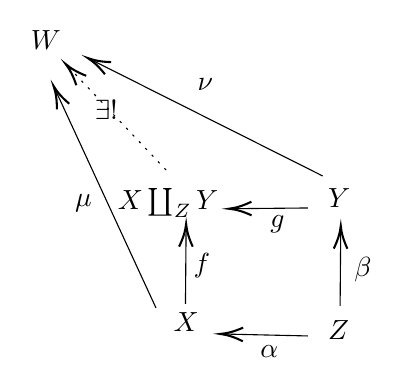
\begin{tikzpicture}[x=0.75pt,y=0.75pt,yscale=-1,xscale=1]
%uncomment if require: \path (0,174); %set diagram left start at 0, and has height of 174

%Straight Lines [id:da9577808904242076] 
\draw    (356.47,150.29) -- (316.21,149.37) ;
\draw [shift={(314.21,149.32)}, rotate = 1.31] [color={rgb, 255:red, 0; green, 0; blue, 0 }  ][line width=0.75]    (10.93,-3.29) .. controls (6.95,-1.4) and (3.31,-0.3) .. (0,0) .. controls (3.31,0.3) and (6.95,1.4) .. (10.93,3.29)   ;
%Straight Lines [id:da6500048244342402] 
\draw    (297.44,134.87) -- (297.75,98.34) ;
\draw [shift={(297.76,96.34)}, rotate = 90.48] [color={rgb, 255:red, 0; green, 0; blue, 0 }  ][line width=0.75]    (10.93,-3.29) .. controls (6.95,-1.4) and (3.31,-0.3) .. (0,0) .. controls (3.31,0.3) and (6.95,1.4) .. (10.93,3.29)   ;
%Straight Lines [id:da7275651749428713] 
\draw    (356.47,88.63) -- (320.33,88.98) ;
\draw [shift={(318.33,89)}, rotate = 359.45] [color={rgb, 255:red, 0; green, 0; blue, 0 }  ][line width=0.75]    (10.93,-3.29) .. controls (6.95,-1.4) and (3.31,-0.3) .. (0,0) .. controls (3.31,0.3) and (6.95,1.4) .. (10.93,3.29)   ;
%Straight Lines [id:da4522671512426313] 
\draw    (371.95,135.84) -- (372.25,99.3) ;
\draw [shift={(372.27,97.3)}, rotate = 90.48] [color={rgb, 255:red, 0; green, 0; blue, 0 }  ][line width=0.75]    (10.93,-3.29) .. controls (6.95,-1.4) and (3.31,-0.3) .. (0,0) .. controls (3.31,0.3) and (6.95,1.4) .. (10.93,3.29)   ;
%Straight Lines [id:da18011941463526604] 
\draw  [dash pattern={on 0.84pt off 2.51pt}]  (288.09,70.33) -- (241.08,20.72) ;
\draw [shift={(239.71,19.27)}, rotate = 46.54] [color={rgb, 255:red, 0; green, 0; blue, 0 }  ][line width=0.75]    (10.93,-3.29) .. controls (6.95,-1.4) and (3.31,-0.3) .. (0,0) .. controls (3.31,0.3) and (6.95,1.4) .. (10.93,3.29)   ;
%Straight Lines [id:da7652339845266762] 
\draw    (283.25,136.8) -- (234.74,31.68) ;
\draw [shift={(233.9,29.86)}, rotate = 65.23] [color={rgb, 255:red, 0; green, 0; blue, 0 }  ][line width=0.75]    (10.93,-3.29) .. controls (6.95,-1.4) and (3.31,-0.3) .. (0,0) .. controls (3.31,0.3) and (6.95,1.4) .. (10.93,3.29)   ;
%Straight Lines [id:da36030228578949086] 
\draw    (363.56,73.22) -- (252.14,17.27) ;
\draw [shift={(250.35,16.38)}, rotate = 26.66] [color={rgb, 255:red, 0; green, 0; blue, 0 }  ][line width=0.75]    (10.93,-3.29) .. controls (6.95,-1.4) and (3.31,-0.3) .. (0,0) .. controls (3.31,0.3) and (6.95,1.4) .. (10.93,3.29)   ;

% Text Node
\draw (290.44,137.87) node [anchor=north west][inner sep=0.75pt]    {$X$};
% Text Node
\draw (364.96,78.14) node [anchor=north west][inner sep=0.75pt]    {$Y$};
% Text Node
\draw (364.96,141.72) node [anchor=north west][inner sep=0.75pt]    {$Z$};
% Text Node
\draw (221.69,2.03) node [anchor=north west][inner sep=0.75pt]    {$W$};
% Text Node
\draw (252.49,35.27) node [anchor=north west][inner sep=0.75pt]    {$\exists !$};
% Text Node
\draw (263.65,78.1) node [anchor=north west][inner sep=0.75pt]    {$X\coprod _{Z} Y$};
% Text Node
\draw (332.24,153.77) node [anchor=north west][inner sep=0.75pt]    {$\alpha $};
% Text Node
\draw (377.56,110.9) node [anchor=north west][inner sep=0.75pt]    {$\beta $};
% Text Node
\draw (300.15,108.97) node [anchor=north west][inner sep=0.75pt]    {$f$};
% Text Node
\draw (337.08,91.15) node [anchor=north west][inner sep=0.75pt]    {$g$};
% Text Node
\draw (243.06,81.03) node [anchor=north west][inner sep=0.75pt]    {$\mu $};
% Text Node
\draw (302.09,25.15) node [anchor=north west][inner sep=0.75pt]    {$\nu $};


\end{tikzpicture}
\end{center}



\begin{example}
     Coproduct for $Sets$ is disjoint union
\end{example}
\begin{remark}
    Suppose $A \rightarrow B$ and $A \rightarrow C$ are two ring morphisms, so in particular $B$ and $C$ are $A$-modules. Recall that $B \otimes_A C$ has a ring structure. Then there is a natural morphism $B \rightarrow B \otimes_A C$ given by $b \mapsto b \otimes 1$. (This is not necessarily an inclusion) Similarly, there is a natural morphism $C \rightarrow B\otimes_A C$. This gives a fibered coproduct on rings, i.e., that
    \begin{center}
        

\tikzset{every picture/.style={line width=0.75pt}} %set default line width to 0.75pt        

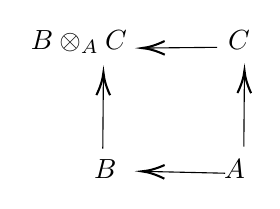
\begin{tikzpicture}[x=0.75pt,y=0.75pt,yscale=-1,xscale=1]
%uncomment if require: \path (0,87); %set diagram left start at 0, and has height of 87

%Straight Lines [id:da23413792064788463] 
\draw    (330.52,72.74) -- (292.37,71.87) ;
\draw [shift={(290.37,71.83)}, rotate = 1.31] [color={rgb, 255:red, 0; green, 0; blue, 0 }  ][line width=0.75]    (10.93,-3.29) .. controls (6.95,-1.4) and (3.31,-0.3) .. (0,0) .. controls (3.31,0.3) and (6.95,1.4) .. (10.93,3.29)   ;
%Straight Lines [id:da8615157391701205] 
\draw    (271.58,60.91) -- (271.87,26.19) ;
\draw [shift={(271.89,24.19)}, rotate = 90.48] [color={rgb, 255:red, 0; green, 0; blue, 0 }  ][line width=0.75]    (10.93,-3.29) .. controls (6.95,-1.4) and (3.31,-0.3) .. (0,0) .. controls (3.31,0.3) and (6.95,1.4) .. (10.93,3.29)   ;
%Straight Lines [id:da35076579391812235] 
\draw    (326.72,12.08) -- (292.48,12.42) ;
\draw [shift={(290.48,12.44)}, rotate = 359.44] [color={rgb, 255:red, 0; green, 0; blue, 0 }  ][line width=0.75]    (10.93,-3.29) .. controls (6.95,-1.4) and (3.31,-0.3) .. (0,0) .. controls (3.31,0.3) and (6.95,1.4) .. (10.93,3.29)   ;
%Straight Lines [id:da4245824711227877] 
\draw    (339.53,59.93) -- (339.82,25.2) ;
\draw [shift={(339.84,23.2)}, rotate = 90.48] [color={rgb, 255:red, 0; green, 0; blue, 0 }  ][line width=0.75]    (10.93,-3.29) .. controls (6.95,-1.4) and (3.31,-0.3) .. (0,0) .. controls (3.31,0.3) and (6.95,1.4) .. (10.93,3.29)   ;

% Text Node
\draw (328.78,64.87) node [anchor=north west][inner sep=0.75pt]    {$A$};
% Text Node
\draw (266.11,64.87) node [anchor=north west][inner sep=0.75pt]    {$B$};
% Text Node
\draw (330.71,2.93) node [anchor=north west][inner sep=0.75pt]    {$C$};
% Text Node
\draw (235.66,2.88) node [anchor=north west][inner sep=0.75pt]    {$B\otimes _{A} C$};


\end{tikzpicture}
    \end{center}
    satisfies the universal property of fibered coproduct
\end{remark}

 \textbf{monomorphism} : a morphism $\pi: X \rightarrow Y$ is a monomorphism if any two morphisms $\mu_1 : Z \rightarrow X$ and $\mu_2 : Z \rightarrow X$ such that $\pi \circ \mu_1 = \pi \circ \mu_2$ must satisfy $\mu_1 = \mu_2$.
In other words, there is at most one way of filling in the dotted arrow so that the diagram
\begin{center}
    

\tikzset{every picture/.style={line width=0.75pt}} %set default line width to 0.75pt        

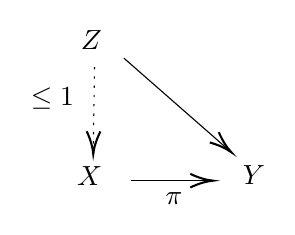
\begin{tikzpicture}[x=0.75pt,y=0.75pt,yscale=-1,xscale=1]
%uncomment if require: \path (0,108); %set diagram left start at 0, and has height of 108

%Straight Lines [id:da4323019017247367] 
\draw  [dash pattern={on 0.84pt off 2.51pt}]  (259.77,25.99) -- (259.2,65.9) ;
\draw [shift={(259.17,67.9)}, rotate = 270.81] [color={rgb, 255:red, 0; green, 0; blue, 0 }  ][line width=0.75]    (10.93,-3.29) .. controls (6.95,-1.4) and (3.31,-0.3) .. (0,0) .. controls (3.31,0.3) and (6.95,1.4) .. (10.93,3.29)   ;
%Straight Lines [id:da7421635920427907] 
\draw    (277.51,80.72) -- (314.85,80.72) ;
\draw [shift={(316.85,80.72)}, rotate = 180] [color={rgb, 255:red, 0; green, 0; blue, 0 }  ][line width=0.75]    (10.93,-3.29) .. controls (6.95,-1.4) and (3.31,-0.3) .. (0,0) .. controls (3.31,0.3) and (6.95,1.4) .. (10.93,3.29)   ;
%Straight Lines [id:da09052392763266837] 
\draw    (273.96,21.71) -- (324.21,65.72) ;
\draw [shift={(325.72,67.04)}, rotate = 221.21] [color={rgb, 255:red, 0; green, 0; blue, 0 }  ][line width=0.75]    (10.93,-3.29) .. controls (6.95,-1.4) and (3.31,-0.3) .. (0,0) .. controls (3.31,0.3) and (6.95,1.4) .. (10.93,3.29)   ;

% Text Node
\draw (250.1,72.84) node [anchor=north west][inner sep=0.75pt]    {$X$};
% Text Node
\draw (330.01,72.27) node [anchor=north west][inner sep=0.75pt]    {$Y$};
% Text Node
\draw (292.81,85.1) node [anchor=north west][inner sep=0.75pt]    {$\pi $};
% Text Node
\draw (251.94,7.27) node [anchor=north west][inner sep=0.75pt]    {$Z$};
% Text Node
\draw (227.85,34.64) node [anchor=north west][inner sep=0.75pt]    {$\leq 1$};


\end{tikzpicture}
\end{center}
commutes — for any object $Z$, the natural map $Mor(Z, X) \rightarrow Mor(Z, Y)$ is an injection
\begin{remark}
    The composition of two monomorphisms is a monomorphism
\end{remark}
\begin{remark}
     A morphism $\pi: X \rightarrow Y$ is a monomorphism $\Leftrightarrow$ the fibered product $X \times_Y X$ exists, and the induced morphism $X \rightarrow X \times_Y X$ is an isomorphism
\end{remark}
\begin{remark}
    If $Y \rightarrow Z$ is a monomorphism, then the morphism $X_1 \times_Y X_2 \rightarrow X_1 \times_Z X_2$ is an isomorphism
\end{remark}

\textbf{epimorphism} : 
a morphism $\pi: Y \rightarrow X$ is a monomorphism if any two morphisms $\mu_1 : X \rightarrow Z$ and $\mu_2 : X \rightarrow Z$ such that $\mu_1 \circ \pi = \mu_2 \circ \pi$ must satisfy $\mu_1 = \mu_2$.
In other words, there is at most one way of filling in the dotted arrow so that the diagram
\begin{center}
    

\tikzset{every picture/.style={line width=0.75pt}} %set default line width to 0.75pt        

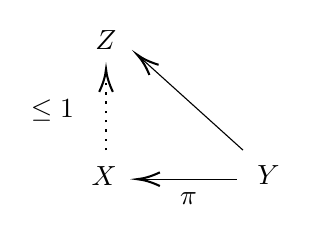
\begin{tikzpicture}[x=0.75pt,y=0.75pt,yscale=-1,xscale=1]
%uncomment if require: \path (0,108); %set diagram left start at 0, and has height of 108

%Straight Lines [id:da4323019017247367] 
\draw  [dash pattern={on 0.84pt off 2.51pt}]  (258.33,66) -- (258.33,29) ;
\draw [shift={(258.33,27)}, rotate = 90] [color={rgb, 255:red, 0; green, 0; blue, 0 }  ][line width=0.75]    (10.93,-3.29) .. controls (6.95,-1.4) and (3.31,-0.3) .. (0,0) .. controls (3.31,0.3) and (6.95,1.4) .. (10.93,3.29)   ;
%Straight Lines [id:da7421635920427907] 
\draw    (321.33,80) -- (275.33,80) ;
\draw [shift={(273.33,80)}, rotate = 360] [color={rgb, 255:red, 0; green, 0; blue, 0 }  ][line width=0.75]    (10.93,-3.29) .. controls (6.95,-1.4) and (3.31,-0.3) .. (0,0) .. controls (3.31,0.3) and (6.95,1.4) .. (10.93,3.29)   ;
%Straight Lines [id:da09052392763266837] 
\draw    (324.33,66) -- (274.82,21.34) ;
\draw [shift={(273.33,20)}, rotate = 42.05] [color={rgb, 255:red, 0; green, 0; blue, 0 }  ][line width=0.75]    (10.93,-3.29) .. controls (6.95,-1.4) and (3.31,-0.3) .. (0,0) .. controls (3.31,0.3) and (6.95,1.4) .. (10.93,3.29)   ;

% Text Node
\draw (250.1,72.84) node [anchor=north west][inner sep=0.75pt]    {$X$};
% Text Node
\draw (330.01,72.27) node [anchor=north west][inner sep=0.75pt]    {$Y$};
% Text Node
\draw (292.81,85.1) node [anchor=north west][inner sep=0.75pt]    {$\pi $};
% Text Node
\draw (251.94,7.27) node [anchor=north west][inner sep=0.75pt]    {$Z$};
% Text Node
\draw (220.85,40.64) node [anchor=north west][inner sep=0.75pt]    {$\leq 1$};


\end{tikzpicture}
\end{center}
commutes — for any object $Z$, the natural map $Mor(X, Z) \rightarrow Mor(Y, Z)$ is an injection
\\

\textbf{Representable functors and Yoneda’s Lemma}
Suppose $A$ is an object of category $\mathscr C$ . For any object $C \in\mathscr C$ , we have a set of morphisms $Mor(C, A)$. If we have a morphism $f : B \rightarrow C$,
we get a map of sets
$$
Mor(C, A) \rightarrow Mor(B, A)
$$
by composition: given a map from $C$ to $A$, we get a map from $B$ to $A$ by precomposing with $f : B \rightarrow C$. Hence this gives a contravariant functor $h_A :\mathscr C \rightarrow Sets$.
Yoneda’s Lemma states that the functor $h_A$ determines $A$ up to unique isomorphism. More precisely:
\begin{lemma}
    (a) Suppose you have two objects $A$ and $A^\prime$ in a category $\mathscr C$ , and morphisms
    $$
    i_C : Mor(C, A) \rightarrow Mor(C, A^\prime)
    $$
    that commute with the maps
    $$
Mor(C, A) \rightarrow Mor(B, A)
$$ for all the $(B,C,f)$ that $f : B\rightarrow C$

Then the $i_C$ (as $C$ ranges over the objects of $C$ ) are induced from a unique morphism $g: A \rightarrow A^\prime$. More precisely, there is a unique morphism $g: A \rightarrow A^\prime$
such that for all $C \in\mathscr C$ , $i_C$ is $u \mapsto g\circ u$
\\
(b) If furthermore the $i_C$ are all bijections, then the resulting $g$ is an isomorphism

(Hint : looking for an element $Mor(A, A^\prime)$. So just plug in $C = A$ to
the first equation, and see where the identity goes
\end{lemma}
There is an analogous statement with the arrows reversed, where instead of maps into $A$, you think of maps from $A$. The role of the contravariant functor $h_A$ is played by the covariant functor $h^A$. The proof is the same (with the arrows reversed)
\begin{lemma}
    (a) Suppose $A$ and $B$ are objects in a category $\mathscr C$. There is a bijection between the natural transformations $h_A \rightarrow h_B$ of covariant functors $\mathscr C \rightarrow Sets$  and the morphisms $B \rightarrow A$
    \\
    (b) Suppose $A$ and $B$ are objects in a category $\mathscr C$. There is a bijection between the natural transformations $h_A \rightarrow h_B$ of contravariant functors $\mathscr C \rightarrow Sets$  and the morphisms $A \rightarrow B$
    
    \textbf{Representable functors} : a contravariant functor $F$ from $\mathscr C$ to $Sets$ is said to be \textbf{representable} if there is a natural isomorphism :
    $$
    \xi : F\cong h_A
    $$
    Thus the representing object A is determined up to unique isomorphism by the pair $(F, \xi)$. There is a similar definition for covariant functors. (The element $\xi^{-1}(id_A) \in F(A)$ is often called the “universal object”; do you see why?)
    \\
    (c) \textbf{Yoneda’s Lemma}. Suppose $F$ is a covariant functor $\mathscr C \rightarrow Sets$, and $A \in\mathscr C$ . There is a bijection between the natural transformations $h^A \rightarrow F$ and $F(A)$
\end{lemma}



\newpage
\subsection{Limits and colimits}

\textbf{Limits}


\textbf{small category} : we say that a category is a small category if the objects and the morphisms are sets

\textbf{index category} : Suppose $\mathscr I$ is any small category, and $\mathscr C$ is any category. Then a functor $F:\mathscr I \rightarrow \mathscr C$
(i.e., with an object $A_i \in \mathscr C$ for each element $i \in \mathscr I$ , and appropriate commuting
morphisms dictated by $\mathscr I$ ) is said to be a \textbf{diagram indexed by} $\mathscr I$. We call $\mathscr I$ an index category
\begin{example}
    if $\square$ is the category in the figure below, and $\mathscr A$ is a category, then a functor $\square \rightarrow \mathscr A$ is precisely the data of a commuting square in $\mathscr A$
    \begin{center}


\tikzset{every picture/.style={line width=0.75pt}} %set default line width to 0.75pt        

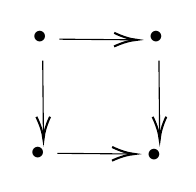
\begin{tikzpicture}[x=0.75pt,y=0.75pt,yscale=-1,xscale=1]
%uncomment if require: \path (0,83); %set diagram left start at 0, and has height of 83

%Straight Lines [id:da36231468328788785] 
\draw    (159,63.67) -- (194.33,63.98) ;
\draw [shift={(196.33,64)}, rotate = 180.51] [color={rgb, 255:red, 0; green, 0; blue, 0 }  ][line width=0.75]    (10.93,-3.29) .. controls (6.95,-1.4) and (3.31,-0.3) .. (0,0) .. controls (3.31,0.3) and (6.95,1.4) .. (10.93,3.29)   ;
%Straight Lines [id:da6364502890495409] 
\draw    (207.98,19.04) -- (208.31,55) ;
\draw [shift={(208.33,57)}, rotate = 269.47] [color={rgb, 255:red, 0; green, 0; blue, 0 }  ][line width=0.75]    (10.93,-3.29) .. controls (6.95,-1.4) and (3.31,-0.3) .. (0,0) .. controls (3.31,0.3) and (6.95,1.4) .. (10.93,3.29)   ;
%Straight Lines [id:da3777619146780913] 
\draw    (151.98,19.04) -- (152.31,55) ;
\draw [shift={(152.33,57)}, rotate = 269.47] [color={rgb, 255:red, 0; green, 0; blue, 0 }  ][line width=0.75]    (10.93,-3.29) .. controls (6.95,-1.4) and (3.31,-0.3) .. (0,0) .. controls (3.31,0.3) and (6.95,1.4) .. (10.93,3.29)   ;
%Straight Lines [id:da45411750213324775] 
\draw    (160,8.67) -- (195.33,8.98) ;
\draw [shift={(197.33,9)}, rotate = 180.51] [color={rgb, 255:red, 0; green, 0; blue, 0 }  ][line width=0.75]    (10.93,-3.29) .. controls (6.95,-1.4) and (3.31,-0.3) .. (0,0) .. controls (3.31,0.3) and (6.95,1.4) .. (10.93,3.29)   ;

% Text Node
\draw (146,3.4) node [anchor=north west][inner sep=0.75pt]    {$\bullet $};
% Text Node
\draw (202,3.4) node [anchor=north west][inner sep=0.75pt]    {$\bullet $};
% Text Node
\draw (145,59.4) node [anchor=north west][inner sep=0.75pt]    {$\bullet $};
% Text Node
\draw (201,60.4) node [anchor=north west][inner sep=0.75pt]    {$\bullet $};


\end{tikzpicture}
    \end{center}
\end{example}
\textbf{limit of the diagram (inverse
limit / projective limit)} : the limit of the diagram is an object $\lim\limits_{\leftarrow \atop \mathscr I}
A_i$ of $\mathscr C$ along with morphisms
$f_j : \lim\limits_{\leftarrow \atop \mathscr I}
A_i
\rightarrow A_j$ for each $j \in \mathscr I$ , such that if $m: j \rightarrow k$ is a morphism in $\mathscr I$, then
\begin{center}
    

\tikzset{every picture/.style={line width=0.75pt}} %set default line width to 0.75pt        

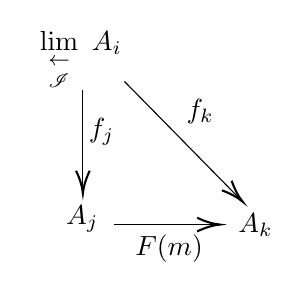
\begin{tikzpicture}[x=0.75pt,y=0.75pt,yscale=-1,xscale=1]
%uncomment if require: \path (0,133); %set diagram left start at 0, and has height of 133

%Straight Lines [id:da36231468328788785] 
\draw    (279.33,97) -- (328.33,97) ;
\draw [shift={(330.33,97)}, rotate = 180] [color={rgb, 255:red, 0; green, 0; blue, 0 }  ][line width=0.75]    (10.93,-3.29) .. controls (6.95,-1.4) and (3.31,-0.3) .. (0,0) .. controls (3.31,0.3) and (6.95,1.4) .. (10.93,3.29)   ;
%Straight Lines [id:da6364502890495409] 
\draw    (284.33,28) -- (339.93,84.57) ;
\draw [shift={(341.33,86)}, rotate = 225.5] [color={rgb, 255:red, 0; green, 0; blue, 0 }  ][line width=0.75]    (10.93,-3.29) .. controls (6.95,-1.4) and (3.31,-0.3) .. (0,0) .. controls (3.31,0.3) and (6.95,1.4) .. (10.93,3.29)   ;
%Straight Lines [id:da3777619146780913] 
\draw    (264.33,32) -- (264.33,80) ;
\draw [shift={(264.33,82)}, rotate = 270] [color={rgb, 255:red, 0; green, 0; blue, 0 }  ][line width=0.75]    (10.93,-3.29) .. controls (6.95,-1.4) and (3.31,-0.3) .. (0,0) .. controls (3.31,0.3) and (6.95,1.4) .. (10.93,3.29)   ;

% Text Node
\draw (255,86.4) node [anchor=north west][inner sep=0.75pt]    {$A_{j}$};
% Text Node
\draw (266,44.4) node [anchor=north west][inner sep=0.75pt]    {$f_{j}$};
% Text Node
\draw (313,35.4) node [anchor=north west][inner sep=0.75pt]    {$f_{k}$};
% Text Node
\draw (238,2.4) node [anchor=north west][inner sep=0.75pt]    {$\lim \limits_{ \begin{array}{l}
\leftarrow \atop
\mathscr{I}
\end{array}} A_{i}$};
% Text Node
\draw (338,90.4) node [anchor=north west][inner sep=0.75pt]    {$A_{k}$};
% Text Node
\draw (288.33,100.4) node [anchor=north west][inner sep=0.75pt]    {$F( m)$};


\end{tikzpicture}
\end{center}
commutes, and this object and maps to each $A_i$ are universal (final) with respect to
this property

More precisely, given any other object $W$ along with maps $g_i : W \rightarrow A_i$ commuting with the $F(m)$ (if $m: j \rightarrow k$ is a morphism in $I$ , then $g_k = F(m)\circ g_j$),
then there is a unique map
\begin{center}
    $g: W \rightarrow \lim\limits_{\leftarrow \atop \mathscr I} A_i$
\end{center}
so that $g_i = f_i \circ g$ for all $i$.
\begin{example}
     fibered product

     If $\mathscr I$ is the partially ordered set:
     \begin{center}


\tikzset{every picture/.style={line width=0.75pt}} %set default line width to 0.75pt        

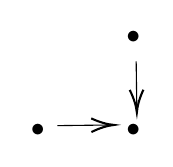
\begin{tikzpicture}[x=0.75pt,y=0.75pt,yscale=-1,xscale=1]
%uncomment if require: \path (0,71); %set diagram left start at 0, and has height of 71

%Straight Lines [id:da24595363596399644] 
\draw    (278,52.33) -- (303.33,52.02) ;
\draw [shift={(305.33,52)}, rotate = 179.3] [color={rgb, 255:red, 0; green, 0; blue, 0 }  ][line width=0.75]    (10.93,-3.29) .. controls (6.95,-1.4) and (3.31,-0.3) .. (0,0) .. controls (3.31,0.3) and (6.95,1.4) .. (10.93,3.29)   ;
%Straight Lines [id:da7606360481536394] 
\draw    (316,21.33) -- (316.31,44) ;
\draw [shift={(316.33,46)}, rotate = 269.23] [color={rgb, 255:red, 0; green, 0; blue, 0 }  ][line width=0.75]    (10.93,-3.29) .. controls (6.95,-1.4) and (3.31,-0.3) .. (0,0) .. controls (3.31,0.3) and (6.95,1.4) .. (10.93,3.29)   ;

% Text Node
\draw (310,5.4) node [anchor=north west][inner sep=0.75pt]    {$\bullet $};
% Text Node
\draw (264,50.4) node [anchor=north west][inner sep=0.75pt]    {$\bullet $};
% Text Node
\draw (310,50.4) node [anchor=north west][inner sep=0.75pt]    {$\bullet $};


\end{tikzpicture}
     \end{center}
     we obtain the fibered product
\end{example}
\begin{example}
     product

     If $\mathscr I$ is\;\; $\bullet\;\;\;\;\bullet$\;\;, we obtain the product
     
     If $\mathscr I$ is a set (i.e., the only morphisms are the identity maps), then the limit is called the \textbf{product} of the $A_i$, and is denoted $\prod_i A_i$. The special case where $\mathscr I$ has two elements is the example of the previous paragraph
\end{example}
\begin{example}
    If $\mathscr I$ has an initial object $e$, then $A_e$ is the limit, and in particular the limit always exists
\end{example}
\begin{example}
    $\bm{p}$\textbf{-adic integers}

    a $p$-adic integer is an element of the inverse limit in the category of the rings :
    \begin{center}
        

\tikzset{every picture/.style={line width=0.75pt}} %set default line width to 0.75pt        

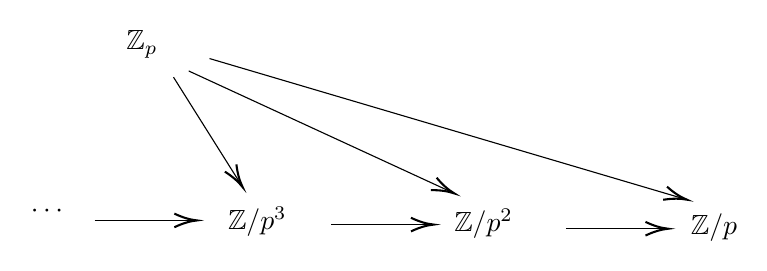
\begin{tikzpicture}[x=0.75pt,y=0.75pt,yscale=-1,xscale=1]
%uncomment if require: \path (0,116); %set diagram left start at 0, and has height of 116

%Straight Lines [id:da6961822570303928] 
\draw    (165,97) -- (212.33,97) ;
\draw [shift={(214.33,97)}, rotate = 180] [color={rgb, 255:red, 0; green, 0; blue, 0 }  ][line width=0.75]    (10.93,-3.29) .. controls (6.95,-1.4) and (3.31,-0.3) .. (0,0) .. controls (3.31,0.3) and (6.95,1.4) .. (10.93,3.29)   ;
%Straight Lines [id:da35013891940605535] 
\draw    (279,99) -- (326.33,99) ;
\draw [shift={(328.33,99)}, rotate = 180] [color={rgb, 255:red, 0; green, 0; blue, 0 }  ][line width=0.75]    (10.93,-3.29) .. controls (6.95,-1.4) and (3.31,-0.3) .. (0,0) .. controls (3.31,0.3) and (6.95,1.4) .. (10.93,3.29)   ;
%Straight Lines [id:da5377937297237212] 
\draw    (392,101) -- (439.33,101) ;
\draw [shift={(441.33,101)}, rotate = 180] [color={rgb, 255:red, 0; green, 0; blue, 0 }  ][line width=0.75]    (10.93,-3.29) .. controls (6.95,-1.4) and (3.31,-0.3) .. (0,0) .. controls (3.31,0.3) and (6.95,1.4) .. (10.93,3.29)   ;
%Straight Lines [id:da37835174036750474] 
\draw    (203,28) -- (235.27,79.31) ;
\draw [shift={(236.33,81)}, rotate = 237.83] [color={rgb, 255:red, 0; green, 0; blue, 0 }  ][line width=0.75]    (10.93,-3.29) .. controls (6.95,-1.4) and (3.31,-0.3) .. (0,0) .. controls (3.31,0.3) and (6.95,1.4) .. (10.93,3.29)   ;
%Straight Lines [id:da5644683697847346] 
\draw    (210.33,25) -- (336.52,83.16) ;
\draw [shift={(338.33,84)}, rotate = 204.75] [color={rgb, 255:red, 0; green, 0; blue, 0 }  ][line width=0.75]    (10.93,-3.29) .. controls (6.95,-1.4) and (3.31,-0.3) .. (0,0) .. controls (3.31,0.3) and (6.95,1.4) .. (10.93,3.29)   ;
%Straight Lines [id:da6539902213448352] 
\draw    (220.33,19) -- (448.42,86.43) ;
\draw [shift={(450.33,87)}, rotate = 196.47] [color={rgb, 255:red, 0; green, 0; blue, 0 }  ][line width=0.75]    (10.93,-3.29) .. controls (6.95,-1.4) and (3.31,-0.3) .. (0,0) .. controls (3.31,0.3) and (6.95,1.4) .. (10.93,3.29)   ;

% Text Node
\draw (179,4.4) node [anchor=north west][inner sep=0.75pt]    {$\mathbb{Z}_{p}$};
% Text Node
\draw (451,92.4) node [anchor=north west][inner sep=0.75pt]    {$\mathbb{Z} /p$};
% Text Node
\draw (337,90.4) node [anchor=north west][inner sep=0.75pt]    {$\mathbb{Z} /p^{2}$};
% Text Node
\draw (228,89.4) node [anchor=north west][inner sep=0.75pt]    {$\mathbb{Z} /p^{3}$};
% Text Node
\draw (133,88.4) node [anchor=north west][inner sep=0.75pt]    {$\cdots $};


\end{tikzpicture}
    \end{center}
\end{example}
\begin{remark}
    In the category $Sets$
    $$
    \left\{(a_i)_{i\in\mathscr I} \in \prod\limlis_i A_i : F(m)(a_j) = a_k\; for\; all\; m \in Mor_{\mathscr I} (j, k) \in Mor(\mathscr I )\right\}
    $$
    along with the obvious projection maps to each $A_i$, is the limit $\lim\limits_{\leftarrow\atop\mathscr I}A_i$
\end{remark}
This clearly also works in the category $Mod_A$ of $A$-modules (in particular $Vec_k$
and $Ab$), as well as $Rings$

From this point of view, $2 + 3p + 2p^2 + \cdots \in\mathbb Z_p$ can be understood as the
sequence $(2, 2 + 3p, 2 + 3p + 2p^2
, \cdots)$
\\

\textbf{colimits (direct
limit / inductive limit / injective limit)}

the colimit of the diagram is an object $\lim\limits_{\rightarrow \atop \mathscr I}
A_i$ of $\mathscr C$ along with morphisms
$f_j : 
A_j
\rightarrow 
\lim\limits_{\rightarrow \atop \mathscr I}
A_i
$ for each $j \in \mathscr I$ , such that if $m: j \rightarrow k$ is a morphism in $\mathscr I$, then
\begin{center}
    

\tikzset{every picture/.style={line width=0.75pt}} %set default line width to 0.75pt        

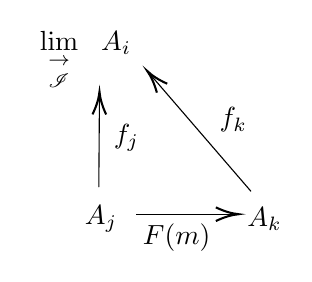
\begin{tikzpicture}[x=0.75pt,y=0.75pt,yscale=-1,xscale=1]
%uncomment if require: \path (0,123); %set diagram left start at 0, and has height of 123

%Straight Lines [id:da6961822570303928] 
\draw    (297,91) -- (344.33,91) ;
\draw [shift={(346.33,91)}, rotate = 180] [color={rgb, 255:red, 0; green, 0; blue, 0 }  ][line width=0.75]    (10.93,-3.29) .. controls (6.95,-1.4) and (3.31,-0.3) .. (0,0) .. controls (3.31,0.3) and (6.95,1.4) .. (10.93,3.29)   ;
%Straight Lines [id:da31174828078942385] 
\draw    (279,78) -- (279.32,34) ;
\draw [shift={(279.33,32)}, rotate = 90.42] [color={rgb, 255:red, 0; green, 0; blue, 0 }  ][line width=0.75]    (10.93,-3.29) .. controls (6.95,-1.4) and (3.31,-0.3) .. (0,0) .. controls (3.31,0.3) and (6.95,1.4) .. (10.93,3.29)   ;
%Straight Lines [id:da044236903932619365] 
\draw    (352.33,80) -- (303.64,23.51) ;
\draw [shift={(302.33,22)}, rotate = 49.24] [color={rgb, 255:red, 0; green, 0; blue, 0 }  ][line width=0.75]    (10.93,-3.29) .. controls (6.95,-1.4) and (3.31,-0.3) .. (0,0) .. controls (3.31,0.3) and (6.95,1.4) .. (10.93,3.29)   ;

% Text Node
\draw (245,1.4) node [anchor=north west][inner sep=0.75pt]    {$\lim \limits_{ \begin{array}{l}
\rightarrow \atop
\mathscr{I}
\end{array}} \ A_{i}$};
% Text Node
\draw (285,46.4) node [anchor=north west][inner sep=0.75pt]    {$f_{j}$};
% Text Node
\draw (336,38.4) node [anchor=north west][inner sep=0.75pt]    {$f_{k}$};
% Text Node
\draw (271,85.4) node [anchor=north west][inner sep=0.75pt]    {$A_{j}$};
% Text Node
\draw (349.33,86.4) node [anchor=north west][inner sep=0.75pt]    {$A_{k}$};
% Text Node
\draw (299,94.4) node [anchor=north west][inner sep=0.75pt]    {$F( m)$};


\end{tikzpicture}
\end{center}
commutes, and this object and maps to each $A_i$ are universal (final) with respect to this property

More precisely, given any other object W along with maps $g_i : A_i \rightarrow W$ commuting with the $F (m)$
(if $m : j \rightarrow k$ is a morphism in $\mathscr I$ , then $g_j =g_k\circ F (m)$ ), then there is a unique map
$g : \lim\limits_{\rightarrow\atop\mathscr I }A_i
\rightarrow 
W
$
so that $g_i = g\circ f_i$ for all $i$
\begin{example}
    The set $5^{-\infty}\mathbb Z$ of rational numbers whose denominators are powers of $5$ is a colimit $\lim\limits_{\rightarrow\atop\mathscr I }5^{-i}\mathbb Z$. More precisely, $5^{-\infty}\mathbb Z$ is the colimit of the diagram
    \begin{center}


\tikzset{every picture/.style={line width=0.75pt}} %set default line width to 0.75pt        

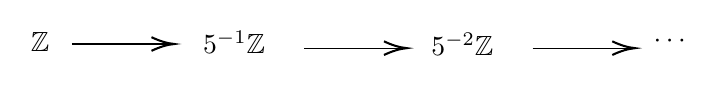
\begin{tikzpicture}[x=0.75pt,y=0.75pt,yscale=-1,xscale=1]
%uncomment if require: \path (0,44); %set diagram left start at 0, and has height of 44

%Straight Lines [id:da6961822570303928] 
\draw    (163,24) -- (210.33,24) ;
\draw [shift={(212.33,24)}, rotate = 180] [color={rgb, 255:red, 0; green, 0; blue, 0 }  ][line width=0.75]    (10.93,-3.29) .. controls (6.95,-1.4) and (3.31,-0.3) .. (0,0) .. controls (3.31,0.3) and (6.95,1.4) .. (10.93,3.29)   ;
%Straight Lines [id:da49044868198843017] 
\draw    (275,26) -- (322.33,26) ;
\draw [shift={(324.33,26)}, rotate = 180] [color={rgb, 255:red, 0; green, 0; blue, 0 }  ][line width=0.75]    (10.93,-3.29) .. controls (6.95,-1.4) and (3.31,-0.3) .. (0,0) .. controls (3.31,0.3) and (6.95,1.4) .. (10.93,3.29)   ;
%Straight Lines [id:da812318655828925] 
\draw    (385,26) -- (432.33,26) ;
\draw [shift={(434.33,26)}, rotate = 180] [color={rgb, 255:red, 0; green, 0; blue, 0 }  ][line width=0.75]    (10.93,-3.29) .. controls (6.95,-1.4) and (3.31,-0.3) .. (0,0) .. controls (3.31,0.3) and (6.95,1.4) .. (10.93,3.29)   ;

% Text Node
\draw (142,17.4) node [anchor=north west][inner sep=0.75pt]    {$\mathbb{Z}$};
% Text Node
\draw (225,16.4) node [anchor=north west][inner sep=0.75pt]    {$5^{-1}\mathbb{Z}$};
% Text Node
\draw (335,17.4) node [anchor=north west][inner sep=0.75pt]    {$5^{-2}\mathbb{Z}$};
% Text Node
\draw (442,18.4) node [anchor=north west][inner sep=0.75pt]    {$\cdots $};


\end{tikzpicture}
    \end{center}
\end{example}
\begin{example}
     coproduct

     If $\mathscr I$ is\;\; $\bullet\;\;\;\;\bullet$\;\;, we obtain the coproduct
     
     If $\mathscr I$ is a set (i.e., the only morphisms are the identity maps), then the colimit is called the \textbf{coproduct} of the $A_i$, and is denoted $\coprod_i A_i$. The special case where $\mathscr I$ has two elements is the example of the previous paragraph
\end{example}
\begin{example}
$\mathbb Q=
\lim\limits_{\rightarrow\atop\mathscr I }\frac{1}{n}\mathbb Z$
\end{example}
\begin{example}
     Define $U\rightarrow V$ iff $V \subset U$, then some subsets of a given set as a colimit. (Dually, the intersection can be interpreted as a limit.) The objects of the category in question are the subsets of the given set.    
\end{example}
\textbf{filtered (directed partially ordered
set / filtered index category)} : 

a nonempty partially ordered set $(S,\geq)$ is filtered (or is said to be a filtered set) if for each $x, y \in S$, there is a $z$ such that $x \geq z$ and $y \geq z$. More generally, a nonempty category $\mathscr I$ is filtered if:

(i) for each $x, y \in \mathscr I$ , there is $a z \in \mathscr I$ and arrows $x \rightarrow z$ and $y \rightarrow z$, and

(ii) for every two arrows $u: x \rightarrow y$ and $v: x \rightarrow y$, there is an arrow $w: y \rightarrow z$
such that $w \circ u = w \circ v$
\begin{remark}
    Suppose $\mathscr I$ is filtered. (We will almost exclusively use the case where $\mathscr I$ is a filtered set.) Recall the symbol $\coprod$ for disjoint union of sets. Then any diagram in Sets indexed by $\mathscr I$ has the following, with the obvious maps to it, as a colimit:
    \begin{center}
        $\left\{(a_i,i)\in \coprod\limits_{i\in\mathscr I} A_i\right\}
        /
        ((a_i, i) \sim (a_j, j)$ if and only if there are $f : A_i \rightarrow A_k$ and $g: A_j \rightarrow A_k$ in the diagram for which $f(a_i) = g(a_j)$ in $A_k$)
    \end{center}
    \label{1.47}
\end{remark}
\begin{example}
     The colimit $\lim\limits_\rightarrow M_i$ in the category of $A$-modules $Mod_A$ can be described as follows. The set underlying $\lim\limits_\rightarrow M_i$ is defined as in Remark \ref{1.47}. To add the elements $m_i \in M_i$ and $m_j \in M_j$, choose an $l \in\mathscr I$ with arrows $u: i \rightarrow l$ and $v: j \rightarrow l$, and then define the sum of $m_i$ and $m_j$ to be $F(u)(m_i) + F(v)(m_j) \in M_l$. The element $m_i \in M_i$ is $0$ if and only if there is some arrow $u: i \rightarrow k$ for which $F(u)(m_i) = 0$, i.e., if it becomes $0$ “later in the diagram”. Last, multiplication by an element of $A$ is defined in the obvious way

     The $A$-module described above is indeed the colimit
\end{example}
\begin{example}
Direct limits exist in the category $(Set)$ and $(Ab)$ of sets and abelian groups. More precisely:

(1) Let $\left(\{A_{i}\}_{i\in I},\,\{\rho_{i j}\}_{i,j\in I}\right)$ be a direct system in $(Set)$. Then 
$\lim\limits_\rightarrow _{i\in I}A_{i} = \prod_{i\in I}A_{i}/\sim,$ 
where $a_{i}\sim a_{j}$ 
if and only if there exists $k\in I$ such that ${i,j}\leq k$ and $\rho_{i k}(a_{i})\,=\,\rho_{j k}(a_{j})$, 
together with the maps $\rho_{i}:A_{i} \rightarrow \prod_{i\in I}A_{i}/\sim$
induced by the inclusions is a direct limit of $(\{A_{i}\}_{i\in I},\{\rho_{i j}\}_{i,j\in I}).$ 

(2) Let $(\{A_{i}\}_{i\in I},\{\rho_{i j}\}_{i,j\in I})$ be a direct system in $(Ab)$. Then $\lim\limits_\rightarrow _{i\in I}A_{i}=\bigoplus_{i\in I}A_{i}/N$  
where
$N$ is the subgroup generated by elements of the form $a_{i}-\rho_{i j}(a_{i})$  together with the maps $\rho_{i}:A_{i} \rightarrow\bigoplus_{i\in I}A_{i}/N$ induced by the inclusions is a direct limit of $(\{A_{i}\}_{i\in I},\{\rho_{i j}\}_{i,j\in I}).$  

(3) Let $(\{A_{i}\}_{i\in I},\{\rho_{i j}\}_{i,j\in I})$ be a direct system in $(Ab)$. Forgetting the group structure, it becomes a direct system in $(Set)$. The induced map $\textstyle{\prod_{i\in I}A_{i}/\sim\to\bigoplus_{i\in I}A_{i}/N}$ 
is a bijection
that identifies the $f_i$
in (1) and (2).

Similarly, if $(\{A_{i}\}_{i\in I},\{\rho_{i j}\}_{i,j\in I})$ is a direct system of modules or rings, then the direct limit exists and the underlying set is the direct limit of the underlying sets.
\end{example}
\begin{example}
     Suppose $S$ is a multiplicative set of integral domain $A$, then $S^{-1}A =\lim\limits_\rightarrow\frac{1}{s}A$ where the limit is over $s \in S$, and in the category of $A$-modules
\end{example}
\begin{example}
    COLIMITS OF $A$-MODULES WITHOUT THE FILTERED CONDITION

    Suppose you are given a diagram of $A$-modules indexed by $\mathscr I : F: \mathscr I \rightarrow Mod_A$, where we let $M_i := F(i)$. Show that the colimit is $\oplus_{i\in\mathscr I}$ Mi modulo the relations $m_i-F(n)(m_i)$ for every $n$: $i \rightarrow j$ in $\mathscr I$ (i.e., for every arrow in the diagram). (Some what more precisely: “modulo” means “quotiented by the submodule generated by”)
\end{example}







\newpage
\subsection{Adjoints}
\textbf{adjoints} :

Two covariant functors $F:\mathscr A \rightarrow \mathscr B$
and $G:\mathscr B \rightarrow \mathscr A$ are adjoint if there is a natural bijection for all $A \in\mathscr A$ and $B \in\mathscr B$
$$
\tau_{AB} : Mor_\mathscr B(F(A), B) \rightarrow Mor_\mathscr A (A, G(B))
$$
We say that $(F, G)$ form an \textbf{adjoint pair}, and that $F$ is \textbf{left-adjoint} to $G$ (and $G$ is
\textbf{right-adjoint} to $F$). We say $F$ is a \textbf{left adjoint} (and $G$ is a \textbf{right adjoint})

 By “natural”
we mean the following. For all $f : A \rightarrow A^\prime$
in $\mathscr A$ , we require
\begin{center}
    

\tikzset{every picture/.style={line width=0.75pt}} %set default line width to 0.75pt        

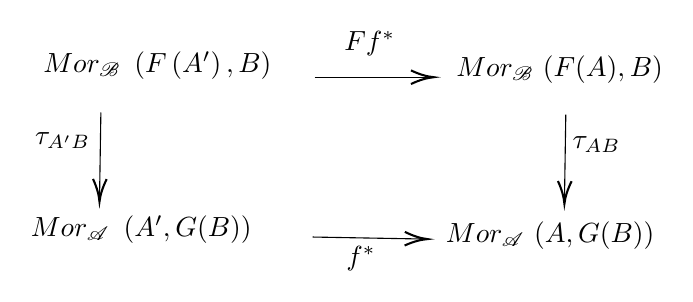
\begin{tikzpicture}[x=0.75pt,y=0.75pt,yscale=-1,xscale=1]
%uncomment if require: \path (0,133); %set diagram left start at 0, and has height of 133

%Straight Lines [id:da6961822570303928] 
\draw    (278,101) -- (331.33,101.96) ;
\draw [shift={(333.33,102)}, rotate = 181.04] [color={rgb, 255:red, 0; green, 0; blue, 0 }  ][line width=0.75]    (10.93,-3.29) .. controls (6.95,-1.4) and (3.31,-0.3) .. (0,0) .. controls (3.31,0.3) and (6.95,1.4) .. (10.93,3.29)   ;
%Straight Lines [id:da49044868198843017] 
\draw    (279,24) -- (334.33,24) ;
\draw [shift={(336.33,24)}, rotate = 180] [color={rgb, 255:red, 0; green, 0; blue, 0 }  ][line width=0.75]    (10.93,-3.29) .. controls (6.95,-1.4) and (3.31,-0.3) .. (0,0) .. controls (3.31,0.3) and (6.95,1.4) .. (10.93,3.29)   ;
%Straight Lines [id:da812318655828925] 
\draw    (176,41) -- (175.36,82) ;
\draw [shift={(175.33,84)}, rotate = 270.89] [color={rgb, 255:red, 0; green, 0; blue, 0 }  ][line width=0.75]    (10.93,-3.29) .. controls (6.95,-1.4) and (3.31,-0.3) .. (0,0) .. controls (3.31,0.3) and (6.95,1.4) .. (10.93,3.29)   ;
%Straight Lines [id:da505294004107123] 
\draw    (400,42) -- (399.36,83) ;
\draw [shift={(399.33,85)}, rotate = 270.89] [color={rgb, 255:red, 0; green, 0; blue, 0 }  ][line width=0.75]    (10.93,-3.29) .. controls (6.95,-1.4) and (3.31,-0.3) .. (0,0) .. controls (3.31,0.3) and (6.95,1.4) .. (10.93,3.29)   ;

% Text Node
\draw (147,10.4) node [anchor=north west][inner sep=0.75pt]    {$Mor_{\mathscr{B}} \ \left( F\left( A^{\prime }\right) ,B\right)$};
% Text Node
\draw (346,12.4) node [anchor=north west][inner sep=0.75pt]    {$Mor_{\mathscr{B}} \ ( F( A) ,B)$};
% Text Node
\draw (141,89.4) node [anchor=north west][inner sep=0.75pt]    {$Mor_{\mathscr{A}} \ \left( A^{\prime } ,G( B)\right)$};
% Text Node
\draw (341,92.4) node [anchor=north west][inner sep=0.75pt]    {$Mor_{\mathscr{A}} \ ( A,G( B))$};
% Text Node
\draw (402,51.4) node [anchor=north west][inner sep=0.75pt]    {$\tau _{AB}$};
% Text Node
\draw (143,49.4) node [anchor=north west][inner sep=0.75pt]    {$\tau _{A^{\prime } B}$};
% Text Node
\draw (293,104.4) node [anchor=north west][inner sep=0.75pt]    {$f^{\ast }$};
% Text Node
\draw (292,0.4) node [anchor=north west][inner sep=0.75pt]    {$Ff^{\ast }$};


\end{tikzpicture}
\end{center}
to commute, and for all $g: B \rightarrow B^\prime$
in $\mathscr B$ we want a similar commutative diagram to commute
\begin{center}
    

\tikzset{every picture/.style={line width=0.75pt}} %set default line width to 0.75pt        

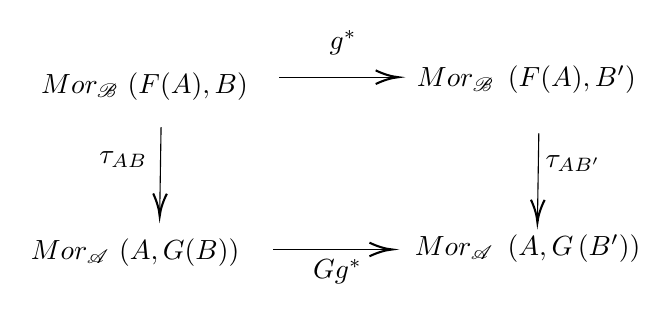
\begin{tikzpicture}[x=0.75pt,y=0.75pt,yscale=-1,xscale=1]
%uncomment if require: \path (0,151); %set diagram left start at 0, and has height of 151

%Straight Lines [id:da505294004107123] 
\draw    (218,46) -- (217.36,87) ;
\draw [shift={(217.33,89)}, rotate = 270.89] [color={rgb, 255:red, 0; green, 0; blue, 0 }  ][line width=0.75]    (10.93,-3.29) .. controls (6.95,-1.4) and (3.31,-0.3) .. (0,0) .. controls (3.31,0.3) and (6.95,1.4) .. (10.93,3.29)   ;
%Straight Lines [id:da8121972938293023] 
\draw    (275,22) -- (330.33,22) ;
\draw [shift={(332.33,22)}, rotate = 180] [color={rgb, 255:red, 0; green, 0; blue, 0 }  ][line width=0.75]    (10.93,-3.29) .. controls (6.95,-1.4) and (3.31,-0.3) .. (0,0) .. controls (3.31,0.3) and (6.95,1.4) .. (10.93,3.29)   ;
%Straight Lines [id:da30431616332359335] 
\draw    (272,105) -- (327.33,105) ;
\draw [shift={(329.33,105)}, rotate = 180] [color={rgb, 255:red, 0; green, 0; blue, 0 }  ][line width=0.75]    (10.93,-3.29) .. controls (6.95,-1.4) and (3.31,-0.3) .. (0,0) .. controls (3.31,0.3) and (6.95,1.4) .. (10.93,3.29)   ;
%Straight Lines [id:da21738862989440144] 
\draw    (400,49) -- (399.36,90) ;
\draw [shift={(399.33,92)}, rotate = 270.89] [color={rgb, 255:red, 0; green, 0; blue, 0 }  ][line width=0.75]    (10.93,-3.29) .. controls (6.95,-1.4) and (3.31,-0.3) .. (0,0) .. controls (3.31,0.3) and (6.95,1.4) .. (10.93,3.29)   ;

% Text Node
\draw (159,18.4) node [anchor=north west][inner sep=0.75pt]    {$Mor_{\mathscr{B}} \ ( F( A) ,B)$};
% Text Node
\draw (154,98.4) node [anchor=north west][inner sep=0.75pt]    {$Mor_{\mathscr{A}} \ ( A,G( B))$};
% Text Node
\draw (187,56.4) node [anchor=north west][inner sep=0.75pt]    {$\tau _{AB}$};
% Text Node
\draw (340,15.4) node [anchor=north west][inner sep=0.75pt]    {$Mor_{\mathscr{B}} \ \left( F( A) ,B^{\prime }\right)$};
% Text Node
\draw (339,96.4) node [anchor=north west][inner sep=0.75pt]    {$Mor_{\mathscr{A}} \ \left( A,G\left( B^{\prime }\right)\right)$};
% Text Node
\draw (402,58.4) node [anchor=north west][inner sep=0.75pt]    {$\tau _{AB^{\prime }}$};
% Text Node
\draw (298,-1.6) node [anchor=north west][inner sep=0.75pt]    {$g^{\ast }$};
% Text Node
\draw (290,108.4) node [anchor=north west][inner sep=0.75pt]    {$Gg^{\ast }$};


\end{tikzpicture}
\end{center}
(Here $f^\ast$ is the map induced by $f : A \rightarrow A^\prime$
, and $Ff^\ast$ is the map induced by $Ff : F(A) \rightarrow F(A^\prime)$)

In fact, we have :
\begin{center}
    

\tikzset{every picture/.style={line width=0.75pt}} %set default line width to 0.75pt        

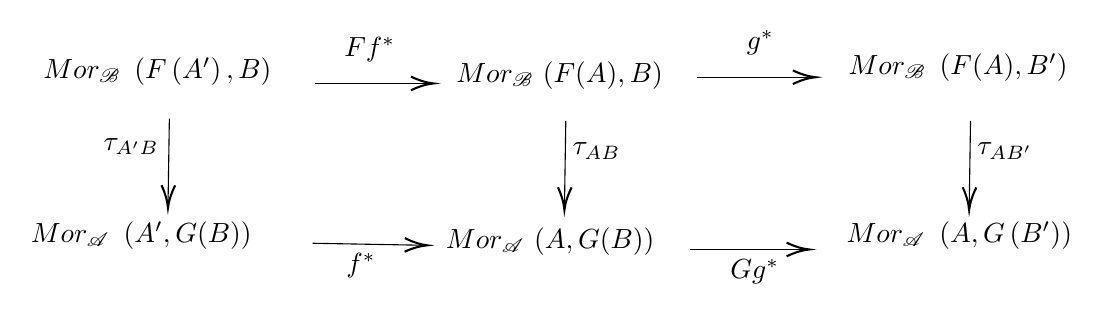
\begin{tikzpicture}[x=0.75pt,y=0.75pt,yscale=-1,xscale=1]
%uncomment if require: \path (0,151); %set diagram left start at 0, and has height of 151

%Straight Lines [id:da6961822570303928] 
\draw    (201,109) -- (254.33,109.96) ;
\draw [shift={(256.33,110)}, rotate = 181.04] [color={rgb, 255:red, 0; green, 0; blue, 0 }  ][line width=0.75]    (10.93,-3.29) .. controls (6.95,-1.4) and (3.31,-0.3) .. (0,0) .. controls (3.31,0.3) and (6.95,1.4) .. (10.93,3.29)   ;
%Straight Lines [id:da49044868198843017] 
\draw    (202,32) -- (257.33,32) ;
\draw [shift={(259.33,32)}, rotate = 180] [color={rgb, 255:red, 0; green, 0; blue, 0 }  ][line width=0.75]    (10.93,-3.29) .. controls (6.95,-1.4) and (3.31,-0.3) .. (0,0) .. controls (3.31,0.3) and (6.95,1.4) .. (10.93,3.29)   ;
%Straight Lines [id:da812318655828925] 
\draw    (132,49) -- (131.36,90) ;
\draw [shift={(131.33,92)}, rotate = 270.89] [color={rgb, 255:red, 0; green, 0; blue, 0 }  ][line width=0.75]    (10.93,-3.29) .. controls (6.95,-1.4) and (3.31,-0.3) .. (0,0) .. controls (3.31,0.3) and (6.95,1.4) .. (10.93,3.29)   ;
%Straight Lines [id:da505294004107123] 
\draw    (323,50) -- (322.36,91) ;
\draw [shift={(322.33,93)}, rotate = 270.89] [color={rgb, 255:red, 0; green, 0; blue, 0 }  ][line width=0.75]    (10.93,-3.29) .. controls (6.95,-1.4) and (3.31,-0.3) .. (0,0) .. controls (3.31,0.3) and (6.95,1.4) .. (10.93,3.29)   ;
%Straight Lines [id:da8121972938293023] 
\draw    (386,29) -- (441.33,29) ;
\draw [shift={(443.33,29)}, rotate = 180] [color={rgb, 255:red, 0; green, 0; blue, 0 }  ][line width=0.75]    (10.93,-3.29) .. controls (6.95,-1.4) and (3.31,-0.3) .. (0,0) .. controls (3.31,0.3) and (6.95,1.4) .. (10.93,3.29)   ;
%Straight Lines [id:da30431616332359335] 
\draw    (383,112) -- (438.33,112) ;
\draw [shift={(440.33,112)}, rotate = 180] [color={rgb, 255:red, 0; green, 0; blue, 0 }  ][line width=0.75]    (10.93,-3.29) .. controls (6.95,-1.4) and (3.31,-0.3) .. (0,0) .. controls (3.31,0.3) and (6.95,1.4) .. (10.93,3.29)   ;
%Straight Lines [id:da21738862989440144] 
\draw    (518,50) -- (517.36,91) ;
\draw [shift={(517.33,93)}, rotate = 270.89] [color={rgb, 255:red, 0; green, 0; blue, 0 }  ][line width=0.75]    (10.93,-3.29) .. controls (6.95,-1.4) and (3.31,-0.3) .. (0,0) .. controls (3.31,0.3) and (6.95,1.4) .. (10.93,3.29)   ;

% Text Node
\draw (70,18.4) node [anchor=north west][inner sep=0.75pt]    {$Mor_{\mathscr{B}} \ \left( F\left( A^{\prime }\right) ,B\right)$};
% Text Node
\draw (269,20.4) node [anchor=north west][inner sep=0.75pt]    {$Mor_{\mathscr{B}} \ ( F( A) ,B)$};
% Text Node
\draw (64,97.4) node [anchor=north west][inner sep=0.75pt]    {$Mor_{\mathscr{A}} \ \left( A^{\prime } ,G( B)\right)$};
% Text Node
\draw (264,100.4) node [anchor=north west][inner sep=0.75pt]    {$Mor_{\mathscr{A}} \ ( A,G( B))$};
% Text Node
\draw (325,59.4) node [anchor=north west][inner sep=0.75pt]    {$\tau _{AB}$};
% Text Node
\draw (99,57.4) node [anchor=north west][inner sep=0.75pt]    {$\tau _{A^{\prime } B}$};
% Text Node
\draw (216,112.4) node [anchor=north west][inner sep=0.75pt]    {$f^{\ast }$};
% Text Node
\draw (215,8.4) node [anchor=north west][inner sep=0.75pt]    {$Ff^{\ast }$};
% Text Node
\draw (458,16.4) node [anchor=north west][inner sep=0.75pt]    {$Mor_{\mathscr{B}} \ \left( F( A) ,B^{\prime }\right)$};
% Text Node
\draw (457,97.4) node [anchor=north west][inner sep=0.75pt]    {$Mor_{\mathscr{A}} \ \left( A,G\left( B^{\prime }\right)\right)$};
% Text Node
\draw (520,59.4) node [anchor=north west][inner sep=0.75pt]    {$\tau _{AB^{\prime }}$};
% Text Node
\draw (409,5.4) node [anchor=north west][inner sep=0.75pt]    {$g^{\ast }$};
% Text Node
\draw (401,115.4) node [anchor=north west][inner sep=0.75pt]    {$Gg^{\ast }$};


\end{tikzpicture}
\end{center}
\begin{remark}
    The map $\tau_{AB}$ has the following properties :
    
    For each $A$ there is a map $\eta_A : A \rightarrow GF(A)$ so that for any $g: F(A) \rightarrow B$, the corresponding $\tau_{AB}(g) : A \rightarrow G(B)$ is given by the composition
    $$
    A \stackrel{\eta_A}{\longrightarrow} GF(A)  \stackrel{Gg}{\longrightarrow}  G(B)
    $$
    
    Similarly, there is a map $\epsilon_B : FG(B) \rightarrow B$ for each $B$ so that for any $f : A \rightarrow G(B)$, the corresponding map $\tau^{-1}_{AB}(f) : F(A) \rightarrow B$ is given by the composition 
    $$
    F(A)  \stackrel{Ff}{\longrightarrow} FG(B)  \stackrel{\epsilon_B}{\longrightarrow} B
    $$
\end{remark}
\begin{Proof}
    \begin{center}
\tikzset{every picture/.style={line width=0.75pt}} %set default line width to 0.75pt        

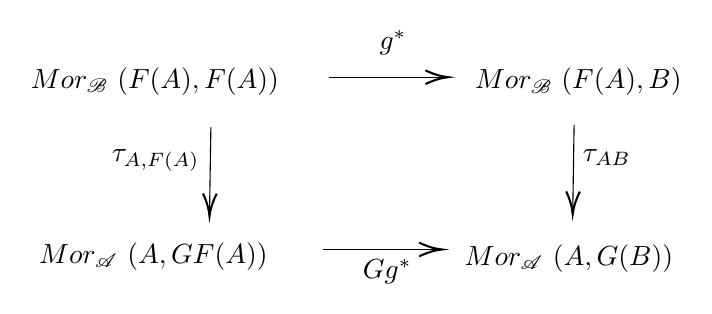
\begin{tikzpicture}[x=0.75pt,y=0.75pt,yscale=-1,xscale=1]
%uncomment if require: \path (0,136); %set diagram left start at 0, and has height of 136

%Straight Lines [id:da505294004107123] 
\draw    (218,46) -- (217.36,87) ;
\draw [shift={(217.33,89)}, rotate = 270.89] [color={rgb, 255:red, 0; green, 0; blue, 0 }  ][line width=0.75]    (10.93,-3.29) .. controls (6.95,-1.4) and (3.31,-0.3) .. (0,0) .. controls (3.31,0.3) and (6.95,1.4) .. (10.93,3.29)   ;
%Straight Lines [id:da8121972938293023] 
\draw    (275,22) -- (330.33,22) ;
\draw [shift={(332.33,22)}, rotate = 180] [color={rgb, 255:red, 0; green, 0; blue, 0 }  ][line width=0.75]    (10.93,-3.29) .. controls (6.95,-1.4) and (3.31,-0.3) .. (0,0) .. controls (3.31,0.3) and (6.95,1.4) .. (10.93,3.29)   ;
%Straight Lines [id:da30431616332359335] 
\draw    (272,105) -- (327.33,105) ;
\draw [shift={(329.33,105)}, rotate = 180] [color={rgb, 255:red, 0; green, 0; blue, 0 }  ][line width=0.75]    (10.93,-3.29) .. controls (6.95,-1.4) and (3.31,-0.3) .. (0,0) .. controls (3.31,0.3) and (6.95,1.4) .. (10.93,3.29)   ;
%Straight Lines [id:da21738862989440144] 
\draw    (393,45) -- (392.36,86) ;
\draw [shift={(392.33,88)}, rotate = 270.89] [color={rgb, 255:red, 0; green, 0; blue, 0 }  ][line width=0.75]    (10.93,-3.29) .. controls (6.95,-1.4) and (3.31,-0.3) .. (0,0) .. controls (3.31,0.3) and (6.95,1.4) .. (10.93,3.29)   ;

% Text Node
\draw (344,16.4) node [anchor=north west][inner sep=0.75pt]    {$Mor_{\mathscr{B}} \ ( F( A) ,B)$};
% Text Node
\draw (339,101.4) node [anchor=north west][inner sep=0.75pt]    {$Mor_{\mathscr{A}} \ ( A,G( B))$};
% Text Node
\draw (396,55.4) node [anchor=north west][inner sep=0.75pt]    {$\tau _{AB}$};
% Text Node
\draw (298,-1.6) node [anchor=north west][inner sep=0.75pt]    {$g^{\ast }$};
% Text Node
\draw (290,108.4) node [anchor=north west][inner sep=0.75pt]    {$Gg^{\ast }$};
% Text Node
\draw (130,16.07) node [anchor=north west][inner sep=0.75pt]    {$Mor_{\mathscr{B}} \ ( F( A) ,F( A))$};
% Text Node
\draw (134,100.4) node [anchor=north west][inner sep=0.75pt]    {$Mor_{\mathscr{A}} \ ( A,GF( A))$};
% Text Node
\draw (169,55.4) node [anchor=north west][inner sep=0.75pt]    {$\tau _{A,F( A)}$};


\end{tikzpicture}
    \end{center}
So $\eta_A=\tau_{A,F(A)}(1_{F(A)})$
\end{Proof}
\begin{example}
    Suppose $M, N$, and $P$ are $A$-modules (where $A$ is a ring). There is a bijection $$
    Hom_A(M\otimes_A N, P)\leftrightarrow Hom_A(M, Hom_A(N, P))
    $$
    
    (Hint : try to use the universal property of $\otimes$)

    $(\cdot) \otimes_A N$ and $Hom_A(N, \cdot)$ are adjoint functors
\end{example}
\begin{example}
    Suppose $B \rightarrow A$ is a morphism of rings. If $M$ is an $A$-module, We can create a $B$-module $M_B$ by considering it as a $B$-module. This gives a functor $\cdot B : Mod_A \rightarrow Mod_B$. Then this functor is right-adjoint to $\cdot \otimes_B A$. In other words, there is a bijection
    $$
     Hom_A(N \otimes_B A,M) \cong Hom_B(N,M_B)
    $$
\end{example}
\begin{example}
    For those familiar with representation theory:
    
Frobenius reciprocity may be understood in terms of adjoints. Suppose $V$ is a
finite-dimensional representation of a finite group $G$, and $W$ is a representation of
a subgroup $H < G$. Then induction and restriction are an adjoint pair $(Ind^G_H, Res^G_H)$ between the category of $G$-modules and the category of $H$-modules
\end{example}
\begin{example}
    The loop space is dual to the suspension of the same space; this duality is sometimes called Eckmann–Hilton duality. The basic observation is that
    $
     [\sum Z,X]\cong[Z,\Omega X]
    $
\end{example}
\begin{example}
    \textbf{groupification of abelian semigroups}
    
    Here is another motivating example: getting an abelian group from an abelian semigroup. (An abelian semigroup is just like an abelian group, except we don’t require an identity or an inverse. Morphisms of abelian semigroups are maps of sets preserving the binary operation. One example is the non-negative integers $\mathbb N$ under addition. Another is the positive integers $\mathbb N^\ast$ under multiplication. You may enjoy groupifying both.) From an abelian semigroup, you can create an abelian group. Here is a formalization of that notion.
    
    A groupification of a semigroup $S$ is a map of abelian semigroups $\pi: S \rightarrow G$ such that $G$ is an abelian group, and any map of abelian semigroups from $S$ to an abelian group $G^\prime$ factors uniquely through $G$:
    \begin{center}
        

\tikzset{every picture/.style={line width=0.75pt}} %set default line width to 0.75pt        

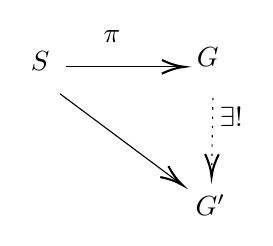
\begin{tikzpicture}[x=0.75pt,y=0.75pt,yscale=-1,xscale=1]
%uncomment if require: \path (0,104); %set diagram left start at 0, and has height of 104

%Straight Lines [id:da7545893166430981] 
\draw    (254,23) -- (309.33,23) ;
\draw [shift={(311.33,23)}, rotate = 180] [color={rgb, 255:red, 0; green, 0; blue, 0 }  ][line width=0.75]    (10.93,-3.29) .. controls (6.95,-1.4) and (3.31,-0.3) .. (0,0) .. controls (3.31,0.3) and (6.95,1.4) .. (10.93,3.29)   ;
%Straight Lines [id:da023849132080275837] 
\draw  [dash pattern={on 0.84pt off 2.51pt}]  (325,38) -- (324.37,74) ;
\draw [shift={(324.33,76)}, rotate = 271.01] [color={rgb, 255:red, 0; green, 0; blue, 0 }  ][line width=0.75]    (10.93,-3.29) .. controls (6.95,-1.4) and (3.31,-0.3) .. (0,0) .. controls (3.31,0.3) and (6.95,1.4) .. (10.93,3.29)   ;
%Straight Lines [id:da8747135574825471] 
\draw    (251.33,36) -- (308.73,78.8) ;
\draw [shift={(310.33,80)}, rotate = 216.71] [color={rgb, 255:red, 0; green, 0; blue, 0 }  ][line width=0.75]    (10.93,-3.29) .. controls (6.95,-1.4) and (3.31,-0.3) .. (0,0) .. controls (3.31,0.3) and (6.95,1.4) .. (10.93,3.29)   ;

% Text Node
\draw (236,14.4) node [anchor=north west][inner sep=0.75pt]    {$S$};
% Text Node
\draw (316,12.4) node [anchor=north west][inner sep=0.75pt]    {$G$};
% Text Node
\draw (315.33,83.4) node [anchor=north west][inner sep=0.75pt]    {$G^{\prime }$};
% Text Node
\draw (271,4.4) node [anchor=north west][inner sep=0.75pt]    {$\pi $};
% Text Node
\draw (327,41.4) node [anchor=north west][inner sep=0.75pt]    {$\exists !$};


\end{tikzpicture}
    \end{center}
    Construct the “groupification functor” $H$ from the category of nonempty abelian semigroups to the category of abelian groups.

    Let $F$ be the forgetful functor from the category of abelian groups $Ab$ to the category of abelian semigroups. Then $H$ is left-adjoint to $F$.
\end{example}
\begin{example}
    $S^{-1}A$-modules are a fully faithful subcategory of the category of $A$-modules (via the obvious inclusion $Mod_{S^{-1}A} \hookrightarrow Mod_A$). Then $Mod_A \rightarrow Mod_{S^{-1}A}$ can be interpreted as an adjoint to the forgetful functor $Mod_{S^{-1}A} \rightarrow ModA$
\end{example}
\begin{remark}
    Here is a table of most of the adjoints that will come up for us.
    \begin{table}[h!]
\begin{center}
    \begin{tabular}{c|c|c|c|c} % <-- Alignments: 1st column left, 2nd middle and 3rd right, with vertical lines in between
      \textbf{situation} 
      & \textbf{category}$\mathscr A$ 
      & \textbf{category}$\mathscr B$ 
      &
      \textbf{left adjoint} 
      $F:\mathscr A \rightarrow \mathscr B$ 
      &
      \textbf{right adjoint}
      $G:\mathscr B \rightarrow\mathscr A$
      \\
      \hline
      $A$-modules &  &  & $(\cdot) \otimes_A N$ & $Hom_A(N, \cdot)$\\
     \hline
      ring maps $B \rightarrow A$ & $Mod_B$ & $Mod_A$ & $(\cdot) \otimes_B$ & $M \rightarrow M_B$
      \\ & & &(extension of scalars) & (restriction of scalars) \\
     \hline
       (pre)sheaves on a & presheaves & sheaves & sheafification & forgetful\\ topological space  $X$  & on $X$ &  on $X$ & &\\
     \hline
      (semi)groups & semigroups & groups & groupification & forgetful \\
     \hline
      sheaves, & sheaves & sheaves & $\pi^{-1}$ & $\pi_\ast$
      \\
      $\pi: X\rightarrow Y$ & on $Y$ & on $X$ & &\\ 
      \hline
      sheaves of abelian & & & & \\ 
      groups or $\mathscr O$-modules, & sheaves & sheaves & $\pi_!$ & $\pi^{-1}$\\
      open embeddings & on $U$ & on $Y$ & &\\
      $\pi: U \hookrightarrow Y$ & & & &\\
      \hline
      ring maps & & & $M \mapsto M_B$ & $N \mapsto$
      \\
      $B \rightarrow A$ & $Mod_A$ & $Mod_B$  & (restriction & $Hom_B(A, N)$
      \\
       & & & of scalars) &
      \\
      \hline
      quasicoherent sheaves, & $QCoh_X$ & $QCoh_Y$ & &
      \\
      affine $\pi: X \rightarrow Y$ & & & $\pi_\ast$ & $\pi^!_{sh}$
      \\
    \end{tabular}
\end{center}
\end{table}
\end{remark}








\newpage
\subsection{Abelian categories}

\textbf{preadditive category} : a category $\mathscr A$ is called preadditive if each morphism set $Mor_\mathscr A (x,y)$ is endowed with the structure of an abelian group such that the compositions
$$
Mor(x,y)\times Mor(y,z)
\rightarrow Mor(x,z)
$$
are bilinear


\textbf{additive functor} : a functor $F:\mathscr A\rightarrow \mathscr B$ of preadditive categories is called additive if and only if $F:Mor(x,y)\rightarrow Mor(F(x),F(y))$ is a homomorphism of abelian groups for all $x,y\in Ob(\mathscr A)$

In particular for every $x,y$ there exists at least one morphism $x\rightarrow y$, namely the zero map. 

Let $0$ be the zero map from $x$ to $y$, by bilinearity, for an arbitrary object of $\mathscr A$ : $z$, $f\in Mor(y,z),g\in Mor(z,x)$, we have $f\circ 0=$the zero map from $x$ to $z$, $0\circ g=$the zero map from $z$ to $y$. (Hint : $f\circ 0=f\circ (0+0)$)
\begin{lemma}
    Let $\mathscr A$ be a preadditive category. Let $x$ be an object of $\mathscr A$. The following are equivalent:

(1) $x$ is an initial object,

(2) $x$ is a final object, and

(3) $id_x=0$ in $Mor_\mathscr A(x,x)$.

Furthermore, if such an object $0$ exists, then a morphism $\alpha:x\rightarrow y$ factors through $0$ if and only if $\alpha=0$.
\end{lemma}
\begin{Proof}
    First assume that $x$ is either (1) initial or (2) final. In both cases, it follows that $Mor(x,x)$ is a trivial abelian group containing $id_x$, thus $id_x=0$ in $Mor(x,x)$, which shows that each of (1) and (2) implies (3).

    Now assume that $id_x=0$ in $Mor(x,x)$. Let $y$ be an arbitrary object of $\mathscr A$ and let $f\in Mor(x,y)$. Denote $C:Mor(x,x)\times Mor(x,y)\rightarrow Mor(x,y)$ the composition map. Then $f=C(0,f)$ and since $C$ is bilinear we have $C(0,f)=0$. Thus $f=0$. Hence $x$ is initial in $\mathscr A$. A similar argument for $f\in Mor(y,x)$ can be used to show that $x$ is also final. Thus (3) implies both (1) and (2).
\end{Proof}
\begin{lemma}
    Let $\mathscr A$ be a preadditive category. Let $x,y\in Ob(\mathscr A)$. If the product $x\times y$ exists, then so does the coproduct $x\coprod y$. If the coproduct $x\coprod y$ exists, then so does the product $x\times y$. In this case also $x\coprod y\cong x\times y$.
\end{lemma}
\begin{Proof}
    Suppose that $z=x\times y$ with projections $p:z\rightarrow x$ and $q:z\rightarrow y$. Denote $i:x\rightarrow z$ the morphism corresponding to $(1,0)$. Denote $j:y\rightarrow z$ the morphism corresponding to $(0,1)$. Thus we have the commutative diagram
    \begin{center}


\tikzset{every picture/.style={line width=0.75pt}} %set default line width to 0.75pt        

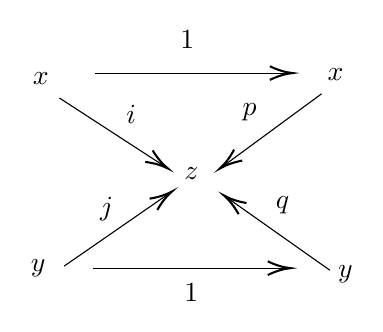
\begin{tikzpicture}[x=0.75pt,y=0.75pt,yscale=-1,xscale=1]
%uncomment if require: \path (0,168); %set diagram left start at 0, and has height of 168

%Straight Lines [id:da9298228644148323] 
\draw    (246,40) -- (296.66,72.91) ;
\draw [shift={(298.33,74)}, rotate = 213.01] [color={rgb, 255:red, 0; green, 0; blue, 0 }  ][line width=0.75]    (10.93,-3.29) .. controls (6.95,-1.4) and (3.31,-0.3) .. (0,0) .. controls (3.31,0.3) and (6.95,1.4) .. (10.93,3.29)   ;
%Straight Lines [id:da438543071434796] 
\draw    (372.33,38) -- (324.95,72.82) ;
\draw [shift={(323.33,74)}, rotate = 323.7] [color={rgb, 255:red, 0; green, 0; blue, 0 }  ][line width=0.75]    (10.93,-3.29) .. controls (6.95,-1.4) and (3.31,-0.3) .. (0,0) .. controls (3.31,0.3) and (6.95,1.4) .. (10.93,3.29)   ;
%Straight Lines [id:da120796274167569] 
\draw    (248.33,121) -- (298.69,86.14) ;
\draw [shift={(300.33,85)}, rotate = 145.3] [color={rgb, 255:red, 0; green, 0; blue, 0 }  ][line width=0.75]    (10.93,-3.29) .. controls (6.95,-1.4) and (3.31,-0.3) .. (0,0) .. controls (3.31,0.3) and (6.95,1.4) .. (10.93,3.29)   ;
%Straight Lines [id:da36477221227795154] 
\draw    (376.33,123) -- (326.97,88.15) ;
\draw [shift={(325.33,87)}, rotate = 35.22] [color={rgb, 255:red, 0; green, 0; blue, 0 }  ][line width=0.75]    (10.93,-3.29) .. controls (6.95,-1.4) and (3.31,-0.3) .. (0,0) .. controls (3.31,0.3) and (6.95,1.4) .. (10.93,3.29)   ;
%Straight Lines [id:da4098899144537018] 
\draw    (263.33,28) -- (356.33,28) ;
\draw [shift={(358.33,28)}, rotate = 180] [color={rgb, 255:red, 0; green, 0; blue, 0 }  ][line width=0.75]    (10.93,-3.29) .. controls (6.95,-1.4) and (3.31,-0.3) .. (0,0) .. controls (3.31,0.3) and (6.95,1.4) .. (10.93,3.29)   ;
%Straight Lines [id:da8447970931374391] 
\draw    (262.33,122) -- (355.33,122) ;
\draw [shift={(357.33,122)}, rotate = 180] [color={rgb, 255:red, 0; green, 0; blue, 0 }  ][line width=0.75]    (10.93,-3.29) .. controls (6.95,-1.4) and (3.31,-0.3) .. (0,0) .. controls (3.31,0.3) and (6.95,1.4) .. (10.93,3.29)   ;

% Text Node
\draw (232,26.4) node [anchor=north west][inner sep=0.75pt]    {$x$};
% Text Node
\draw (374,24.4) node [anchor=north west][inner sep=0.75pt]    {$x$};
% Text Node
\draw (231,116.4) node [anchor=north west][inner sep=0.75pt]    {$y$};
% Text Node
\draw (379,119.4) node [anchor=north west][inner sep=0.75pt]    {$y$};
% Text Node
\draw (305,72.4) node [anchor=north west][inner sep=0.75pt]    {$z$};
% Text Node
\draw (277,42.4) node [anchor=north west][inner sep=0.75pt]    {$i$};
% Text Node
\draw (333,41.4) node [anchor=north west][inner sep=0.75pt]    {$p$};
% Text Node
\draw (264.33,86.4) node [anchor=north west][inner sep=0.75pt]    {$j$};
% Text Node
\draw (349,86.4) node [anchor=north west][inner sep=0.75pt]    {$q$};
% Text Node
\draw (303,6.4) node [anchor=north west][inner sep=0.75pt]    {$1$};
% Text Node
\draw (305,128.4) node [anchor=north west][inner sep=0.75pt]    {$1$};


\end{tikzpicture}
    \end{center}
    where the diagonal compositions are zero. It follows that $i\circ p+j\circ q:z\rightarrow z$ is the identity since it is a morphism which upon composing with $p$ gives $p$ and upon composing with $q$ gives $q$. Suppose given morphisms $a:x\rightarrow w$ and $b:y\rightarrow w$. Then we can form the map $a\circ p+b\circ q:z\rightarrow w$. In this way we get a bijection $Mor(z,w)=Mor(x,w)\times Mor(y,w)$ which show that $z=x\coprod y$.
\end{Proof}


\textbf{direct sum $x\oplus y$} : given a pair of objects $x,y$ in a preadditive category $\mathscr A$, the direct sum $x\oplus y$ of $x$ and $y$ is the direct product $x\times y$ endowed with the morphisms $i,j,p,q$ as in the Lemma above.
\begin{remark}
    Note that the proof of Lemma above shows that given $p$ and $q$ the morphisms $i, j$ are uniquely determined by the rules $p\circ i=id_x, q\circ j=id_y, p\circ j=0, q\circ i=0$. Moreover, we automatically have $i\circ p+j\circ q=id_{x\oplus y}$. Similarly, given $i, j$ the morphisms $p$ and $q$ are uniquely determined. Finally, given objects $x,y,z$ and morphisms $i:x\rightarrow z, j:y\rightarrow z, p:z\rightarrow x$ and $q:z\rightarrow y$ such that $p\circ i=id_x, q\circ j=id_y, p\circ j=0, q\circ i=0$ and $i\circ p+j\circ q=id_z$, then $z$ is the direct sum of $x$ and $y$ with the four morphisms equal to $i,j,p,q$.
\end{remark}
\begin{lemma}
    Let $\mathscr A,\mathscr B$ be preadditive categories. Let $F:\mathscr A \rightarrow \mathscr B$ be an additive functor. Then $F$ transforms direct sums to direct sums and zero to zero.
\end{lemma}
\begin{Proof}
    Suppose $F$ is additive. A direct sum $z$ of $x$ and $y$ is characterized by having morphisms $i:x\rightarrow z, j:y\rightarrow z, p:z\rightarrow x$ and $q:z\rightarrow y$ such that $p\circ i=id_x, q\circ j=id_y, p\circ j=0, q\circ i=0$ and $i\circ p+j\circ q=id_z$, according to Remark above. Clearly $F(x),F(y),F(z)$ and the morphisms $F(i),F(j),F(p),F(q)$ satisfy exactly the same relations (by additivity) and we see that $F(z)$ is a direct sum of $F(x)$ and $F(y)$. Hence, $F$ transforms direct sums to direct sums.
\end{Proof}
\\

\textbf{additive category} : a category $\mathscr C$ is said to be additive if it satisfies the following properties.
\\
Ad1. For each $A, B \in\mathscr C$ , $Mor(A, B)$ is an abelian group, such that composition
of morphisms 

distributes over addition (bilinear)
\\
Ad2. $\mathscr C$ has a zero object, denoted $0$. (This is an object that is simultaneously
an initial object and a 

final object)
\\
Ad3. It has products of two objects (a product $A \times B$ for any pair of objects),
and hence by induction, 

products of any finite number of objects
\\

In an additive category, the morphisms are often called \textbf{homomorphisms}, and $Mor$ is denoted by $Hom$. In fact, this notation $Hom$ is a good indication that you’re
working in an additive category 

 The $0$-morphism in the abelian group $Hom(A, B)$ is the composition $A \rightarrow 0 \rightarrow B$. (We also remark that the notion
of $0$-morphism thus makes sense in any category with a $0$-object)
\\

Let $\mathscr A$ be a preadditive category. Let $f:x\rightarrow y$ be a morphism

\textbf{kernel} : a kernel of $f$ is a morphism $i:z\rightarrow x$ such that (a) $f\circ i=0$ and (b) for any $i^\prime:z^\prime\rightarrow x$ such that $f\circ i^\prime=0$ there exists a unique morphism $g:z^\prime\rightarrow z$ such that $i^\prime=i\circ g$.
\begin{center}


\tikzset{every picture/.style={line width=0.75pt}} %set default line width to 0.75pt        

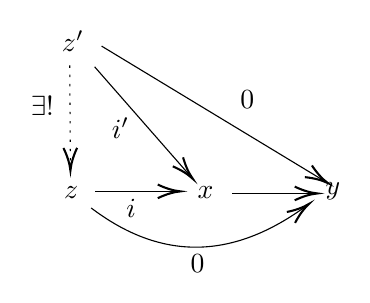
\begin{tikzpicture}[x=0.75pt,y=0.75pt,yscale=-1,xscale=1]
%uncomment if require: \path (0,153); %set diagram left start at 0, and has height of 153

%Straight Lines [id:da9298228644148323] 
\draw    (258,28) -- (304.01,80.5) ;
\draw [shift={(305.33,82)}, rotate = 228.76] [color={rgb, 255:red, 0; green, 0; blue, 0 }  ][line width=0.75]    (10.93,-3.29) .. controls (6.95,-1.4) and (3.31,-0.3) .. (0,0) .. controls (3.31,0.3) and (6.95,1.4) .. (10.93,3.29)   ;
%Straight Lines [id:da120796274167569] 
\draw    (261.33,18) -- (368.62,82.96) ;
\draw [shift={(370.33,84)}, rotate = 211.2] [color={rgb, 255:red, 0; green, 0; blue, 0 }  ][line width=0.75]    (10.93,-3.29) .. controls (6.95,-1.4) and (3.31,-0.3) .. (0,0) .. controls (3.31,0.3) and (6.95,1.4) .. (10.93,3.29)   ;
%Straight Lines [id:da8447970931374391] 
\draw    (324.33,89) -- (363.33,89) ;
\draw [shift={(365.33,89)}, rotate = 180] [color={rgb, 255:red, 0; green, 0; blue, 0 }  ][line width=0.75]    (10.93,-3.29) .. controls (6.95,-1.4) and (3.31,-0.3) .. (0,0) .. controls (3.31,0.3) and (6.95,1.4) .. (10.93,3.29)   ;
%Straight Lines [id:da7361556826668192] 
\draw    (258.33,88) -- (297.33,88) ;
\draw [shift={(299.33,88)}, rotate = 180] [color={rgb, 255:red, 0; green, 0; blue, 0 }  ][line width=0.75]    (10.93,-3.29) .. controls (6.95,-1.4) and (3.31,-0.3) .. (0,0) .. controls (3.31,0.3) and (6.95,1.4) .. (10.93,3.29)   ;
%Curve Lines [id:da7373729681739103] 
\draw    (256.33,96) .. controls (286.36,118.77) and (320.64,123.9) .. (360.13,94.89) ;
\draw [shift={(361.33,94)}, rotate = 143.13] [color={rgb, 255:red, 0; green, 0; blue, 0 }  ][line width=0.75]    (10.93,-3.29) .. controls (6.95,-1.4) and (3.31,-0.3) .. (0,0) .. controls (3.31,0.3) and (6.95,1.4) .. (10.93,3.29)   ;
%Straight Lines [id:da04052099629562478] 
\draw  [dash pattern={on 0.84pt off 2.51pt}]  (246,27.33) -- (246.32,76) ;
\draw [shift={(246.33,78)}, rotate = 269.62] [color={rgb, 255:red, 0; green, 0; blue, 0 }  ][line width=0.75]    (10.93,-3.29) .. controls (6.95,-1.4) and (3.31,-0.3) .. (0,0) .. controls (3.31,0.3) and (6.95,1.4) .. (10.93,3.29)   ;

% Text Node
\draw (306.33,84.4) node [anchor=north west][inner sep=0.75pt]    {$x$};
% Text Node
\draw (368,82.4) node [anchor=north west][inner sep=0.75pt]    {$y$};
% Text Node
\draw (242,84.4) node [anchor=north west][inner sep=0.75pt]    {$z$};
% Text Node
\draw (272,90.4) node [anchor=north west][inner sep=0.75pt]    {$i$};
% Text Node
\draw (241,9.4) node [anchor=north west][inner sep=0.75pt]    {$z^{\prime }$};
% Text Node
\draw (265,51.4) node [anchor=north west][inner sep=0.75pt]    {$i^{\prime }$};
% Text Node
\draw (327,38.4) node [anchor=north west][inner sep=0.75pt]    {$0$};
% Text Node
\draw (303,117.4) node [anchor=north west][inner sep=0.75pt]    {$0$};
% Text Node
\draw (226,40.73) node [anchor=north west][inner sep=0.75pt]    {$\exists !$};


\end{tikzpicture}
\end{center}
The kernel
is written $ker f \rightarrow x$
The kernel of $f : x \rightarrow y$ is the limit of the diagram
\begin{center}
    

\tikzset{every picture/.style={line width=0.75pt}} %set default line width to 0.75pt        

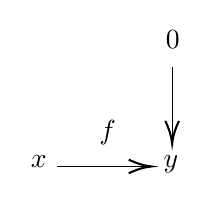
\begin{tikzpicture}[x=0.75pt,y=0.75pt,yscale=-1,xscale=1]
%uncomment if require: \path (0,100); %set diagram left start at 0, and has height of 100

%Straight Lines [id:da05301542023450745] 
\draw    (278,72) -- (321.33,72) ;
\draw [shift={(323.33,72)}, rotate = 180] [color={rgb, 255:red, 0; green, 0; blue, 0 }  ][line width=0.75]    (10.93,-3.29) .. controls (6.95,-1.4) and (3.31,-0.3) .. (0,0) .. controls (3.31,0.3) and (6.95,1.4) .. (10.93,3.29)   ;
%Straight Lines [id:da7010985713087403] 
\draw    (333.33,24) -- (333.33,59) ;
\draw [shift={(333.33,61)}, rotate = 270] [color={rgb, 255:red, 0; green, 0; blue, 0 }  ][line width=0.75]    (10.93,-3.29) .. controls (6.95,-1.4) and (3.31,-0.3) .. (0,0) .. controls (3.31,0.3) and (6.95,1.4) .. (10.93,3.29)   ;

% Text Node
\draw (264,65.4) node [anchor=north west][inner sep=0.75pt]    {$x$};
% Text Node
\draw (328,65.4) node [anchor=north west][inner sep=0.75pt]    {$y$};
% Text Node
\draw (297,48.4) node [anchor=north west][inner sep=0.75pt]    {$f$};
% Text Node
\draw (329,5.4) node [anchor=north west][inner sep=0.75pt]    {$0$};


\end{tikzpicture}
\end{center}

\textbf{cokernel} : a cokernel of $f$ is a morphism $p:y\rightarrow z$ such that (a) $p\circ f=0$ and (b) for any $p^\prime :y\rightarrow z^\prime$ such that $p^\prime\circ f=0$ there exists a unique morphism $g:z\rightarrow z^\prime$ such that $p^\prime=g\circ p$.
\begin{center}


\tikzset{every picture/.style={line width=0.75pt}} %set default line width to 0.75pt        

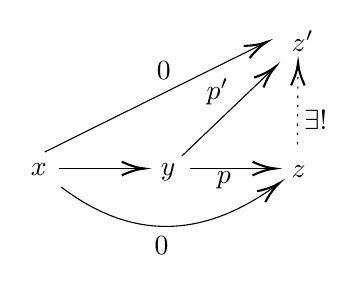
\begin{tikzpicture}[x=0.75pt,y=0.75pt,yscale=-1,xscale=1]
%uncomment if require: \path (0,128); %set diagram left start at 0, and has height of 128

%Straight Lines [id:da9298228644148323] 
\draw    (308.33,67) -- (351.89,25.38) ;
\draw [shift={(353.33,24)}, rotate = 136.3] [color={rgb, 255:red, 0; green, 0; blue, 0 }  ][line width=0.75]    (10.93,-3.29) .. controls (6.95,-1.4) and (3.31,-0.3) .. (0,0) .. controls (3.31,0.3) and (6.95,1.4) .. (10.93,3.29)   ;
%Straight Lines [id:da120796274167569] 
\draw    (242.33,65) -- (347.54,12.89) ;
\draw [shift={(349.33,12)}, rotate = 153.65] [color={rgb, 255:red, 0; green, 0; blue, 0 }  ][line width=0.75]    (10.93,-3.29) .. controls (6.95,-1.4) and (3.31,-0.3) .. (0,0) .. controls (3.31,0.3) and (6.95,1.4) .. (10.93,3.29)   ;
%Straight Lines [id:da8447970931374391] 
\draw    (249.33,73) -- (288.33,73) ;
\draw [shift={(290.33,73)}, rotate = 180] [color={rgb, 255:red, 0; green, 0; blue, 0 }  ][line width=0.75]    (10.93,-3.29) .. controls (6.95,-1.4) and (3.31,-0.3) .. (0,0) .. controls (3.31,0.3) and (6.95,1.4) .. (10.93,3.29)   ;
%Straight Lines [id:da7361556826668192] 
\draw    (312.33,73) -- (351.33,73) ;
\draw [shift={(353.33,73)}, rotate = 180] [color={rgb, 255:red, 0; green, 0; blue, 0 }  ][line width=0.75]    (10.93,-3.29) .. controls (6.95,-1.4) and (3.31,-0.3) .. (0,0) .. controls (3.31,0.3) and (6.95,1.4) .. (10.93,3.29)   ;
%Curve Lines [id:da7373729681739103] 
\draw    (250.33,82) .. controls (280.36,104.77) and (314.64,109.9) .. (354.13,80.89) ;
\draw [shift={(355.33,80)}, rotate = 143.13] [color={rgb, 255:red, 0; green, 0; blue, 0 }  ][line width=0.75]    (10.93,-3.29) .. controls (6.95,-1.4) and (3.31,-0.3) .. (0,0) .. controls (3.31,0.3) and (6.95,1.4) .. (10.93,3.29)   ;
%Straight Lines [id:da04052099629562478] 
\draw  [dash pattern={on 0.84pt off 2.51pt}]  (364,61.33) -- (364.32,24) ;
\draw [shift={(364.33,22)}, rotate = 90.49] [color={rgb, 255:red, 0; green, 0; blue, 0 }  ][line width=0.75]    (10.93,-3.29) .. controls (6.95,-1.4) and (3.31,-0.3) .. (0,0) .. controls (3.31,0.3) and (6.95,1.4) .. (10.93,3.29)   ;

% Text Node
\draw (234.33,69.4) node [anchor=north west][inner sep=0.75pt]    {$x$};
% Text Node
\draw (297,69.4) node [anchor=north west][inner sep=0.75pt]    {$y$};
% Text Node
\draw (360,70.4) node [anchor=north west][inner sep=0.75pt]    {$z$};
% Text Node
\draw (360,5.4) node [anchor=north west][inner sep=0.75pt]    {$z^{\prime }$};
% Text Node
\draw (295,20.4) node [anchor=north west][inner sep=0.75pt]    {$0$};
% Text Node
\draw (294,104.4) node [anchor=north west][inner sep=0.75pt]    {$0$};
% Text Node
\draw (366,43.73) node [anchor=north west][inner sep=0.75pt]    {$\exists !$};
% Text Node
\draw (324,73.4) node [anchor=north west][inner sep=0.75pt]    {$p$};
% Text Node
\draw (319,28.4) node [anchor=north west][inner sep=0.75pt]    {$p^{\prime }$};


\end{tikzpicture}
\end{center}
The cokernel of $f : x \rightarrow y$ is the colimit of the diagram
\begin{center}
    

\tikzset{every picture/.style={line width=0.75pt}} %set default line width to 0.75pt        

\begin{tikzpicture}[x=0.75pt,y=0.75pt,yscale=-1,xscale=1]
%uncomment if require: \path (0,111); %set diagram left start at 0, and has height of 111

%Straight Lines [id:da05301542023450745] 
\draw    (287,28) -- (330.33,28) ;
\draw [shift={(332.33,28)}, rotate = 180] [color={rgb, 255:red, 0; green, 0; blue, 0 }  ][line width=0.75]    (10.93,-3.29) .. controls (6.95,-1.4) and (3.31,-0.3) .. (0,0) .. controls (3.31,0.3) and (6.95,1.4) .. (10.93,3.29)   ;
%Straight Lines [id:da7010985713087403] 
\draw    (278.33,41) -- (278.33,76) ;
\draw [shift={(278.33,78)}, rotate = 270] [color={rgb, 255:red, 0; green, 0; blue, 0 }  ][line width=0.75]    (10.93,-3.29) .. controls (6.95,-1.4) and (3.31,-0.3) .. (0,0) .. controls (3.31,0.3) and (6.95,1.4) .. (10.93,3.29)   ;

% Text Node
\draw (273,21.4) node [anchor=north west][inner sep=0.75pt]    {$x$};
% Text Node
\draw (337,21.4) node [anchor=north west][inner sep=0.75pt]    {$y$};
% Text Node
\draw (304,8.4) node [anchor=north west][inner sep=0.75pt]    {$f$};
% Text Node
\draw (274,84.4) node [anchor=north west][inner sep=0.75pt]    {$0$};


\end{tikzpicture}
\end{center}

\textbf{coimage} : if a kernel of $f$ exists, then a coimage of $f$ is a cokernel for the morphism $ker(f)\rightarrow x$. If a kernel and coimage exist then we denote this $x\rightarrow Coim(f)$.

\textbf{image} : if a cokernel of $f$ exists, then the image of $f$ is a kernel of the morphism $y\rightarrow coker(f)$. If a cokernel and image of $f$ exist then we denote this $Im(f)\rightarrow y$.
\begin{lemma}
    Let $\mathscr C$ be a preadditive category. Let $f:x\rightarrow y$ be a morphism in $\mathscr C$.

(1) If a kernel of $f$ exists, then this kernel is a monomorphism.

(2) If a cokernel of $f$ exists, then this cokernel is an epimorphism.

(3) If a kernel and coimage of $f$ exist, then the coimage is an epimorphism.

(4) If a cokernel and image of $f$ exist, then the image is a monomorphism.
\end{lemma}
\begin{lemma}
    Let $f:x\rightarrow y$ be a morphism in a preadditive category such that the kernel, cokernel, image and coimage all exist. Then $f$ can be factored uniquely as $$
    x\rightarrow Coim(f)\rightarrow Im(f)\rightarrow y
    $$
\end{lemma}

If $i: A \rightarrow B$ is a monomorphism, then we say that $A$ is a \textbf{subobject} of $B$, where the map $i$ is implicit. There is also the notion of \textbf{quotient object}, defined dually to subobject
\\

\textbf{abelian category} : an abelian category is an additive category satisfying three additional properties :

(1) Every map has a kernel and cokernel

(2) Every monomorphism is the kernel of its cokernel

(3) Every epimorphism is the cokernel of its kernel
\\

\textbf{quotient} : the cokernel of a monomorphism is called the quotient. The quotient of a
monomorphism $A \rightarrow B$ is often denoted $B/A$ (with the map from B implicit)
\begin{theorem}
Freyd-Mitchell Embedding Theorem: 

If $\mathscr C$ is an abelian category such that $Hom(X, Y)$ is a set for all $X, Y \in\mathscr C$, then there is a ring $A$ and an exact, fully faithful
functor from $\mathscr C$ into $Mod_A$, which embeds $\mathscr C$ as a full subcategory

In the sense that $Hom_\mathscr A(X, Y) \cong Hom_A(M, N)$

(Unfortunately, the ring $A$ need not be commutative)
\end{theorem}

The upshot is that to prove something about a diagram in some abelian category, we may assume that it is a diagram of modules over some ring, and we may then “diagram-chase” elements. Moreover, any fact about kernels, cokernels, and so on that holds in $Mod_A$ holds in any abelian category)
\\

\textbf{Complexes, exactness, and homology}
(In this entire discussion, we assume we are working in an abelian category.)
We say a sequence :
\begin{equation}
    \cdots \rightarrow A \xrightarrow{f} B \xrightarrow{g} C  \rightarrow \cdots
    \label{equation 1.5.1}
\end{equation}
is a \textbf{complex at} $B$ if $g \circ f = 0$, and is \textbf{exact at} $B$ if $ker g = im f$. (More specifically,
$g$ has a kernel that is an image of $f$. Exactness at $B$ implies being a complex at $B$)
\begin{lemma}
    The above sequence \ref{equation 1.5.1} is exact at $B$ if and only if $Coker(f) = Coim(g)$
\end{lemma}
A sequence is a \textbf{complex} (resp. \textbf{exact}) if it is a complex (resp.
exact) at each (internal) term. 

A \textbf{short exact sequence} is an exact sequence with
five terms, the first and last of which are zeros -- in other words, an exact sequence
of the form :
$$
0
\rightarrow A \rightarrow B \rightarrow C  \rightarrow 0
$$

\begin{lemma}
Fix an abelian category $\mathscr A$. In this category,

(i) $0 \rightarrow A \xrightarrow{f} B$ is exact if and only if $A \xrightarrow{f} B$ is a monomorphism. In this sense, $f=Im(f)$

(ii) $A \xrightarrow{f} B \rightarrow 0$ is exact if and only if $A \xrightarrow{f} B$ is an epimorphism. In this sense, $f=Coim(f)$

(iii) $0 \rightarrow A \rightarrow B \rightarrow 0$ is exact if and only if $A \rightarrow B$ is an isomorphism

(iv) $0 \rightarrow A \xrightarrow{f} B \xrightarrow{g} C$ is exact if and only if $f$ is a kernel of $g$

(V) $A \xrightarrow{f} B \xrightarrow{g} C  \rightarrow 0$ s exact if and only if $g$ is a cokernel of $f$
\end{lemma}
\begin{Proof}
    (i) The cokernel of $0 \rightarrow A$ is the identity map $A \xrightarrow{1_A} A$, which has as kernel $0 \rightarrow A$. So the image of $0 \rightarrow A$ is $0 \rightarrow A$. Thus $0 \rightarrow A \rightarrow B$ is exact if and only if $0 \rightarrow A$ is the kernel of $A \rightarrow B$.

    So we are showing that being a monomorphism is the same as having kernel $0 \rightarrow A$. Suppose first that $A \xrightarrow{f} B$ has kernel $0 \rightarrow A$. Let $g, h$ be two morphisms $Z \rightarrow A$ so that $f \circ g = f \circ h$. Then, by linearity, $f \circ (g − h) = 0$. By the universal property of kernels, $g − h$ factors through $0 \rightarrow A$, so $g - h$ must be the zero morphism. This implies $g = h$, so the defining property of monomorphisms is verified.

    Conversely, suppose $A \xrightarrow{f} B$ is a monomorphism. Suppose $g : Z \rightarrow A$ is a morphism so that $f \circ g = 0$. Note that there is another map with this property, namely the zero morphism, $0 : Z \rightarrow A$. Since $f$ is a monomorphism, $g = 0$. It follows that $g$ factors uniquely through $0 \rightarrow A$. Since $g$ was arbitrary, this verifies that $0 \rightarrow A$ has the universal property of the kernel.
    
(Note: So far, we have only used that $\mathscr A$ is additive and kernels and cokernels
exist.)

(ii) Duality.

(iii) Suppose first that $A \rightarrow B$ is an isomorphism. Then $A \rightarrow B$ is both monic and epic,
so the sequence is exact by parts (i) and (ii).

Suppose conversely that $0 \rightarrow A \rightarrow B \rightarrow 0$ is exact. Then $B \rightarrow 0$ is the cokernel
of $A \rightarrow B$ and $0 \rightarrow A$ is the kernel of $A \rightarrow B$. This makes the image of $A \rightarrow B$ the
morphism $id_B : B \rightarrow B$ and the coimage of $A \rightarrow B$ the morphism $id_A : A \rightarrow A$. 

From (i) and (ii), we can get $f$ is both a monomorphism and an epimorphism. By definition of abelian category, $f$ is  the kernel of its cokernel. So the image of $A\rightarrow B$ is $f : A\rightarrow B$. So $f$ is an isomorphism.

\end{Proof}

\textbf{homology} : If (\ref{equation 1.5.1}) is a complex at $B$, then its homology at $B$ (often denoted by $H$) is
$ker g / im f$. (More precisely, there is some monomorphism $im f \rightarrow ker g$, and that $H$ is the cokernel of this monomorphism.) Therefore, (\ref{equation 1.5.1}) is exact at $B$ if and only if its homology at $B$ is $0$.
We say that elements of $ker g$ are the \textbf{cycles}, and
elements of $im f$ are the \textbf{boundaries} (so homology is “cycles mod boundaries”).

If the complex is indexed in decreasing order, the indices are often written as subscripts, and $H_i$ is the homology at $A_{i+1} \rightarrow A_i \rightarrow A_{i-1}$. If the complex is indexed
in increasing order, the indices are often written as superscripts, and the homology
$H^i$ at $A^{i-1} \rightarrow A^i \rightarrow A^{i+1}$
is often called \textbf{cohomology}.

An exact sequence
\begin{equation}
    A^\bullet\; :
    \;\;
    \cdots \rightarrow A^{i-1} \xrightarrow{f^{i-1}}
    A^{i}
    \xrightarrow{f^{i}}
    A^{i+1}
    \xrightarrow{f^{i+1}}
    \cdots
\end{equation}
can be “factored” into short exact sequences
$$
    0\rightarrow
    ker\;f^i
    \rightarrow
    A^{i}
    \rightarrow
    ker\;f^{i+1}
    \rightarrow
    0
$$
More generally, if (\ref{equation 1.5.1}) is assumed only to be a complex, then it can be
“factored” into short exact sequences.
\begin{equation}
\begin{split}
    &0\rightarrow
    ker\;f^i
    \rightarrow
    A^{i}
    \rightarrow
    im\;f^{i}
    \rightarrow
    0
    \\    
    &0\rightarrow
    im\;f^{i-1}
    \rightarrow
    ker\;f^i
    \rightarrow
    H^i(A^\bullet)
    \rightarrow
    0
    \label{equation 1.5.3}
\end{split}
\end{equation}
We also have :
\begin{equation}
\begin{split}
    &0\rightarrow
    im\;f^i
    \rightarrow
    A^{i+1}
    \rightarrow
    coker\;f^{i}
    \rightarrow
    0
    \\    
    &0\rightarrow
    H^i(A^\bullet)    
    \rightarrow
    coker\;f^{i-1}
    \rightarrow
    im\;f^{i}
    \rightarrow
    0
    \label{equation 1.5.4}
\end{split}
\end{equation}
(These are somehow dual to (\ref{equation 1.5.3}))
\begin{remark}
    Suppose
    $$
    0
    \xrightarrow{d^0}
    A^1
    \xrightarrow{d^1}
    \cdots
    \xrightarrow{d^{n-1}}
    A^n
    \xrightarrow{d^n}
    0
    $$
    is a complex of finite-dimensional $k$-vector spaces (often called $A^\bullet$ for short).
    
    Define $h^i(A^\bullet) := dim\; H^i(A^\bullet)$.

     Then $\sum(-1)^i dim A^i =\sum(-1)^ih^i(A^\bullet)$. In particular, if $A^\bullet$ is exact, then $\sum(-1)^i dim\; A^i = 0$.
\end{remark}
\begin{remark}
    Suppose $\mathscr C$ is an abelian category. Define the category $Com_\mathscr C$ of complexes as follows. The objects are infinite complexes
    \begin{equation}
    A^\bullet\; :
    \;\;
    \cdots \rightarrow A^{i-1} \xrightarrow{f^{i-1}}
    A^{i}
    \xrightarrow{f^{i}}
    A^{i+1}
    \xrightarrow{f^{i+1}}
    \cdots
    \end{equation}
    in $\mathscr C$ , and the morphisms $A^\bullet \rightarrow B^\bullet$ are commuting diagrams
    \begin{equation}
    \begin{split}    
    \cdots \rightarrow &A^{i-1} \xrightarrow{f^{i-1}}
    A^{i}
    \xrightarrow{f^{i}}
    A^{i+1}
    \xrightarrow{f^{i+1}}
    \cdots
    \\
    &\downarrow     \quad\quad\quad\quad\;
    \downarrow 
    \quad\quad\enspace
    \downarrow
    \\
    \cdots \rightarrow &B^{i-1} \xrightarrow{g^{i-1}}
    B^{i}
    \xrightarrow{g^{i}}
    B^{i+1}
    \xrightarrow{g^{i+1}}
    \cdots        
    \end{split}
    \label{equation 1.5.6}
    \end{equation}        
    Then $Com_\mathscr C$ is an abelian category.
    
     (Remark for experts: Essentially the same argument shows that the $\mathscr C^\mathscr I$ is an abelian category for any small category $\mathscr I$ and any abelian category $\mathscr C$. This immediately implies that the category of presheaves on a topological space $X$ with values in an abelian category $\mathscr C$ is automatically an abelian category)
\end{remark}
\begin{remark}
    (\ref{equation 1.5.6}) induces a map of homology $H^i(A^\bullet) \rightarrow H^i(B^\bullet)$
    
    Furthermore, $H^i$ is a covariant functor $Com_\mathscr C \rightarrow \mathscr C$
\end{remark}
\begin{theorem}
     \textbf{(Long exact sequence)}. -- A short exact sequence of complexes
    \begin{center}


\tikzset{every picture/.style={line width=0.75pt}} %set default line width to 0.75pt        

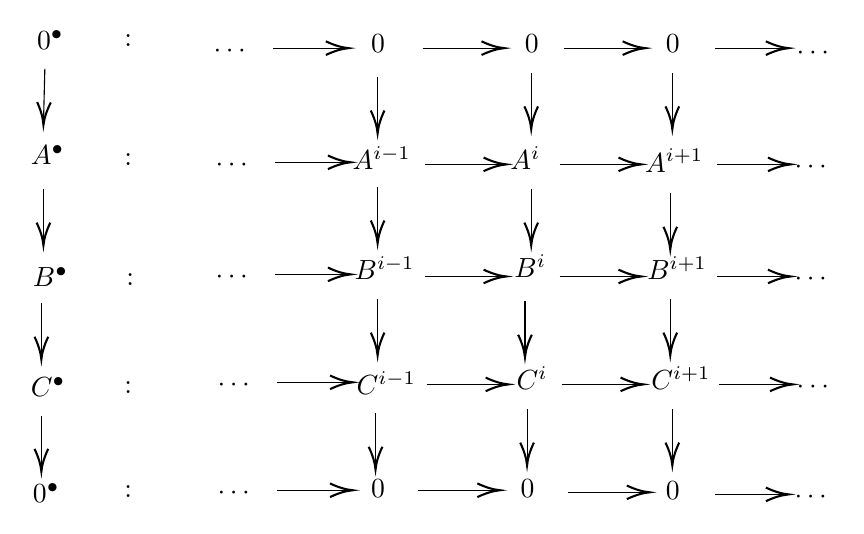
\begin{tikzpicture}[x=0.75pt,y=0.75pt,yscale=-1,xscale=1]
%uncomment if require: \path (0,254); %set diagram left start at 0, and has height of 254

%Straight Lines [id:da8645194871677973] 
\draw    (243,11) -- (277.33,11) ;
\draw [shift={(279.33,11)}, rotate = 180] [color={rgb, 255:red, 0; green, 0; blue, 0 }  ][line width=0.75]    (10.93,-3.29) .. controls (6.95,-1.4) and (3.31,-0.3) .. (0,0) .. controls (3.31,0.3) and (6.95,1.4) .. (10.93,3.29)   ;
%Straight Lines [id:da14343889261413945] 
\draw    (456,11) -- (489.33,11) ;
\draw [shift={(491.33,11)}, rotate = 180] [color={rgb, 255:red, 0; green, 0; blue, 0 }  ][line width=0.75]    (10.93,-3.29) .. controls (6.95,-1.4) and (3.31,-0.3) .. (0,0) .. controls (3.31,0.3) and (6.95,1.4) .. (10.93,3.29)   ;
%Straight Lines [id:da5592636038840972] 
\draw    (315,11) -- (352.33,11) ;
\draw [shift={(354.33,11)}, rotate = 180] [color={rgb, 255:red, 0; green, 0; blue, 0 }  ][line width=0.75]    (10.93,-3.29) .. controls (6.95,-1.4) and (3.31,-0.3) .. (0,0) .. controls (3.31,0.3) and (6.95,1.4) .. (10.93,3.29)   ;
%Straight Lines [id:da6520635846526797] 
\draw    (383,11) -- (420.33,11) ;
\draw [shift={(422.33,11)}, rotate = 180] [color={rgb, 255:red, 0; green, 0; blue, 0 }  ][line width=0.75]    (10.93,-3.29) .. controls (6.95,-1.4) and (3.31,-0.3) .. (0,0) .. controls (3.31,0.3) and (6.95,1.4) .. (10.93,3.29)   ;
%Straight Lines [id:da14995671346447237] 
\draw    (133,21) -- (132.38,46) ;
\draw [shift={(132.33,48)}, rotate = 271.41] [color={rgb, 255:red, 0; green, 0; blue, 0 }  ][line width=0.75]    (10.93,-3.29) .. controls (6.95,-1.4) and (3.31,-0.3) .. (0,0) .. controls (3.31,0.3) and (6.95,1.4) .. (10.93,3.29)   ;
%Straight Lines [id:da19250192469880933] 
\draw    (244,66) -- (278.33,66) ;
\draw [shift={(280.33,66)}, rotate = 180] [color={rgb, 255:red, 0; green, 0; blue, 0 }  ][line width=0.75]    (10.93,-3.29) .. controls (6.95,-1.4) and (3.31,-0.3) .. (0,0) .. controls (3.31,0.3) and (6.95,1.4) .. (10.93,3.29)   ;
%Straight Lines [id:da05180228053065772] 
\draw    (457,67) -- (490.33,67) ;
\draw [shift={(492.33,67)}, rotate = 180] [color={rgb, 255:red, 0; green, 0; blue, 0 }  ][line width=0.75]    (10.93,-3.29) .. controls (6.95,-1.4) and (3.31,-0.3) .. (0,0) .. controls (3.31,0.3) and (6.95,1.4) .. (10.93,3.29)   ;
%Straight Lines [id:da7595347158892853] 
\draw    (316,67) -- (353.33,67) ;
\draw [shift={(355.33,67)}, rotate = 180] [color={rgb, 255:red, 0; green, 0; blue, 0 }  ][line width=0.75]    (10.93,-3.29) .. controls (6.95,-1.4) and (3.31,-0.3) .. (0,0) .. controls (3.31,0.3) and (6.95,1.4) .. (10.93,3.29)   ;
%Straight Lines [id:da6539664754382708] 
\draw    (381,67) -- (418.33,67) ;
\draw [shift={(420.33,67)}, rotate = 180] [color={rgb, 255:red, 0; green, 0; blue, 0 }  ][line width=0.75]    (10.93,-3.29) .. controls (6.95,-1.4) and (3.31,-0.3) .. (0,0) .. controls (3.31,0.3) and (6.95,1.4) .. (10.93,3.29)   ;
%Straight Lines [id:da5921198521921414] 
\draw    (244,120) -- (278.33,120) ;
\draw [shift={(280.33,120)}, rotate = 180] [color={rgb, 255:red, 0; green, 0; blue, 0 }  ][line width=0.75]    (10.93,-3.29) .. controls (6.95,-1.4) and (3.31,-0.3) .. (0,0) .. controls (3.31,0.3) and (6.95,1.4) .. (10.93,3.29)   ;
%Straight Lines [id:da6601579132726794] 
\draw    (457,121) -- (490.33,121) ;
\draw [shift={(492.33,121)}, rotate = 180] [color={rgb, 255:red, 0; green, 0; blue, 0 }  ][line width=0.75]    (10.93,-3.29) .. controls (6.95,-1.4) and (3.31,-0.3) .. (0,0) .. controls (3.31,0.3) and (6.95,1.4) .. (10.93,3.29)   ;
%Straight Lines [id:da4845338764596987] 
\draw    (316,121) -- (353.33,121) ;
\draw [shift={(355.33,121)}, rotate = 180] [color={rgb, 255:red, 0; green, 0; blue, 0 }  ][line width=0.75]    (10.93,-3.29) .. controls (6.95,-1.4) and (3.31,-0.3) .. (0,0) .. controls (3.31,0.3) and (6.95,1.4) .. (10.93,3.29)   ;
%Straight Lines [id:da6382417103188525] 
\draw    (381,121) -- (418.33,121) ;
\draw [shift={(420.33,121)}, rotate = 180] [color={rgb, 255:red, 0; green, 0; blue, 0 }  ][line width=0.75]    (10.93,-3.29) .. controls (6.95,-1.4) and (3.31,-0.3) .. (0,0) .. controls (3.31,0.3) and (6.95,1.4) .. (10.93,3.29)   ;
%Straight Lines [id:da8121956689279992] 
\draw    (245,172) -- (279.33,172) ;
\draw [shift={(281.33,172)}, rotate = 180] [color={rgb, 255:red, 0; green, 0; blue, 0 }  ][line width=0.75]    (10.93,-3.29) .. controls (6.95,-1.4) and (3.31,-0.3) .. (0,0) .. controls (3.31,0.3) and (6.95,1.4) .. (10.93,3.29)   ;
%Straight Lines [id:da06487234681938703] 
\draw    (458,173) -- (491.33,173) ;
\draw [shift={(493.33,173)}, rotate = 180] [color={rgb, 255:red, 0; green, 0; blue, 0 }  ][line width=0.75]    (10.93,-3.29) .. controls (6.95,-1.4) and (3.31,-0.3) .. (0,0) .. controls (3.31,0.3) and (6.95,1.4) .. (10.93,3.29)   ;
%Straight Lines [id:da5593355075825763] 
\draw    (317,173) -- (354.33,173) ;
\draw [shift={(356.33,173)}, rotate = 180] [color={rgb, 255:red, 0; green, 0; blue, 0 }  ][line width=0.75]    (10.93,-3.29) .. controls (6.95,-1.4) and (3.31,-0.3) .. (0,0) .. controls (3.31,0.3) and (6.95,1.4) .. (10.93,3.29)   ;
%Straight Lines [id:da5640442444975957] 
\draw    (382,173) -- (419.33,173) ;
\draw [shift={(421.33,173)}, rotate = 180] [color={rgb, 255:red, 0; green, 0; blue, 0 }  ][line width=0.75]    (10.93,-3.29) .. controls (6.95,-1.4) and (3.31,-0.3) .. (0,0) .. controls (3.31,0.3) and (6.95,1.4) .. (10.93,3.29)   ;
%Straight Lines [id:da4479927483270092] 
\draw    (245,224) -- (279.33,224) ;
\draw [shift={(281.33,224)}, rotate = 180] [color={rgb, 255:red, 0; green, 0; blue, 0 }  ][line width=0.75]    (10.93,-3.29) .. controls (6.95,-1.4) and (3.31,-0.3) .. (0,0) .. controls (3.31,0.3) and (6.95,1.4) .. (10.93,3.29)   ;
%Straight Lines [id:da6791895411397444] 
\draw    (456,226) -- (489.33,226) ;
\draw [shift={(491.33,226)}, rotate = 180] [color={rgb, 255:red, 0; green, 0; blue, 0 }  ][line width=0.75]    (10.93,-3.29) .. controls (6.95,-1.4) and (3.31,-0.3) .. (0,0) .. controls (3.31,0.3) and (6.95,1.4) .. (10.93,3.29)   ;
%Straight Lines [id:da7065032029894522] 
\draw    (313,224) -- (350.33,224) ;
\draw [shift={(352.33,224)}, rotate = 180] [color={rgb, 255:red, 0; green, 0; blue, 0 }  ][line width=0.75]    (10.93,-3.29) .. controls (6.95,-1.4) and (3.31,-0.3) .. (0,0) .. controls (3.31,0.3) and (6.95,1.4) .. (10.93,3.29)   ;
%Straight Lines [id:da8451024002180556] 
\draw    (385,225) -- (422.33,225) ;
\draw [shift={(424.33,225)}, rotate = 180] [color={rgb, 255:red, 0; green, 0; blue, 0 }  ][line width=0.75]    (10.93,-3.29) .. controls (6.95,-1.4) and (3.31,-0.3) .. (0,0) .. controls (3.31,0.3) and (6.95,1.4) .. (10.93,3.29)   ;
%Straight Lines [id:da5133582881986114] 
\draw    (131.33,188) -- (131.33,213) ;
\draw [shift={(131.33,215)}, rotate = 270] [color={rgb, 255:red, 0; green, 0; blue, 0 }  ][line width=0.75]    (10.93,-3.29) .. controls (6.95,-1.4) and (3.31,-0.3) .. (0,0) .. controls (3.31,0.3) and (6.95,1.4) .. (10.93,3.29)   ;
%Straight Lines [id:da6998653783413475] 
\draw    (132.33,79) -- (132.33,104) ;
\draw [shift={(132.33,106)}, rotate = 270] [color={rgb, 255:red, 0; green, 0; blue, 0 }  ][line width=0.75]    (10.93,-3.29) .. controls (6.95,-1.4) and (3.31,-0.3) .. (0,0) .. controls (3.31,0.3) and (6.95,1.4) .. (10.93,3.29)   ;
%Straight Lines [id:da4957730115101293] 
\draw    (131.33,134) -- (131.33,159) ;
\draw [shift={(131.33,161)}, rotate = 270] [color={rgb, 255:red, 0; green, 0; blue, 0 }  ][line width=0.75]    (10.93,-3.29) .. controls (6.95,-1.4) and (3.31,-0.3) .. (0,0) .. controls (3.31,0.3) and (6.95,1.4) .. (10.93,3.29)   ;
%Straight Lines [id:da5370456659602689] 
\draw    (293.33,25) -- (293.33,50) ;
\draw [shift={(293.33,52)}, rotate = 270] [color={rgb, 255:red, 0; green, 0; blue, 0 }  ][line width=0.75]    (10.93,-3.29) .. controls (6.95,-1.4) and (3.31,-0.3) .. (0,0) .. controls (3.31,0.3) and (6.95,1.4) .. (10.93,3.29)   ;
%Straight Lines [id:da6846809162912886] 
\draw    (293.33,78) -- (293.33,103) ;
\draw [shift={(293.33,105)}, rotate = 270] [color={rgb, 255:red, 0; green, 0; blue, 0 }  ][line width=0.75]    (10.93,-3.29) .. controls (6.95,-1.4) and (3.31,-0.3) .. (0,0) .. controls (3.31,0.3) and (6.95,1.4) .. (10.93,3.29)   ;
%Straight Lines [id:da8809596844372669] 
\draw    (293.33,132) -- (293.33,157) ;
\draw [shift={(293.33,159)}, rotate = 270] [color={rgb, 255:red, 0; green, 0; blue, 0 }  ][line width=0.75]    (10.93,-3.29) .. controls (6.95,-1.4) and (3.31,-0.3) .. (0,0) .. controls (3.31,0.3) and (6.95,1.4) .. (10.93,3.29)   ;
%Straight Lines [id:da730074376191542] 
\draw    (292.33,187) -- (292.33,212) ;
\draw [shift={(292.33,214)}, rotate = 270] [color={rgb, 255:red, 0; green, 0; blue, 0 }  ][line width=0.75]    (10.93,-3.29) .. controls (6.95,-1.4) and (3.31,-0.3) .. (0,0) .. controls (3.31,0.3) and (6.95,1.4) .. (10.93,3.29)   ;
%Straight Lines [id:da8818375557756255] 
\draw    (367.33,23) -- (367.33,48) ;
\draw [shift={(367.33,50)}, rotate = 270] [color={rgb, 255:red, 0; green, 0; blue, 0 }  ][line width=0.75]    (10.93,-3.29) .. controls (6.95,-1.4) and (3.31,-0.3) .. (0,0) .. controls (3.31,0.3) and (6.95,1.4) .. (10.93,3.29)   ;
%Straight Lines [id:da5135390301365392] 
\draw    (435.33,23) -- (435.33,48) ;
\draw [shift={(435.33,50)}, rotate = 270] [color={rgb, 255:red, 0; green, 0; blue, 0 }  ][line width=0.75]    (10.93,-3.29) .. controls (6.95,-1.4) and (3.31,-0.3) .. (0,0) .. controls (3.31,0.3) and (6.95,1.4) .. (10.93,3.29)   ;
%Straight Lines [id:da8827883869457773] 
\draw    (365.33,185) -- (365.33,210) ;
\draw [shift={(365.33,212)}, rotate = 270] [color={rgb, 255:red, 0; green, 0; blue, 0 }  ][line width=0.75]    (10.93,-3.29) .. controls (6.95,-1.4) and (3.31,-0.3) .. (0,0) .. controls (3.31,0.3) and (6.95,1.4) .. (10.93,3.29)   ;
%Straight Lines [id:da4353568693508203] 
\draw    (435.33,185) -- (435.33,210) ;
\draw [shift={(435.33,212)}, rotate = 270] [color={rgb, 255:red, 0; green, 0; blue, 0 }  ][line width=0.75]    (10.93,-3.29) .. controls (6.95,-1.4) and (3.31,-0.3) .. (0,0) .. controls (3.31,0.3) and (6.95,1.4) .. (10.93,3.29)   ;
%Straight Lines [id:da9035017922103015] 
\draw    (364.33,133) -- (364.33,158) ;
\draw [shift={(364.33,160)}, rotate = 270] [color={rgb, 255:red, 0; green, 0; blue, 0 }  ][line width=0.75]    (10.93,-3.29) .. controls (6.95,-1.4) and (3.31,-0.3) .. (0,0) .. controls (3.31,0.3) and (6.95,1.4) .. (10.93,3.29)   ;
%Straight Lines [id:da11606095926676874] 
\draw    (434.33,132) -- (434.33,157) ;
\draw [shift={(434.33,159)}, rotate = 270] [color={rgb, 255:red, 0; green, 0; blue, 0 }  ][line width=0.75]    (10.93,-3.29) .. controls (6.95,-1.4) and (3.31,-0.3) .. (0,0) .. controls (3.31,0.3) and (6.95,1.4) .. (10.93,3.29)   ;
%Straight Lines [id:da42182976272978934] 
\draw    (367.33,79) -- (367.33,104) ;
\draw [shift={(367.33,106)}, rotate = 270] [color={rgb, 255:red, 0; green, 0; blue, 0 }  ][line width=0.75]    (10.93,-3.29) .. controls (6.95,-1.4) and (3.31,-0.3) .. (0,0) .. controls (3.31,0.3) and (6.95,1.4) .. (10.93,3.29)   ;
%Straight Lines [id:da7139194659982615] 
\draw    (434.33,81) -- (434.33,106) ;
\draw [shift={(434.33,108)}, rotate = 270] [color={rgb, 255:red, 0; green, 0; blue, 0 }  ][line width=0.75]    (10.93,-3.29) .. controls (6.95,-1.4) and (3.31,-0.3) .. (0,0) .. controls (3.31,0.3) and (6.95,1.4) .. (10.93,3.29)   ;

% Text Node
\draw (128,1.4) node [anchor=north west][inner sep=0.75pt]    {$0^{\bullet }$};
% Text Node
\draw (170,3.4) node [anchor=north west][inner sep=0.75pt]    {$:$};
% Text Node
\draw (213,8.4) node [anchor=north west][inner sep=0.75pt]    {$\cdots $};
% Text Node
\draw (289,3.4) node [anchor=north west][inner sep=0.75pt]    {$0$};
% Text Node
\draw (363,3.4) node [anchor=north west][inner sep=0.75pt]    {$0$};
% Text Node
\draw (431,3.4) node [anchor=north west][inner sep=0.75pt]    {$0$};
% Text Node
\draw (494,9.4) node [anchor=north west][inner sep=0.75pt]    {$\cdots $};
% Text Node
\draw (125,56.4) node [anchor=north west][inner sep=0.75pt]    {$A^{\bullet }$};
% Text Node
\draw (126,115.4) node [anchor=north west][inner sep=0.75pt]    {$B^{\bullet }$};
% Text Node
\draw (125,168.4) node [anchor=north west][inner sep=0.75pt]    {$C^{\bullet }$};
% Text Node
\draw (171,118.4) node [anchor=north west][inner sep=0.75pt]    {$:$};
% Text Node
\draw (170,60.4) node [anchor=north west][inner sep=0.75pt]    {$:$};
% Text Node
\draw (170,170.4) node [anchor=north west][inner sep=0.75pt]    {$:$};
% Text Node
\draw (214,63.4) node [anchor=north west][inner sep=0.75pt]    {$\cdots $};
% Text Node
\draw (493,64.4) node [anchor=north west][inner sep=0.75pt]    {$\cdots $};
% Text Node
\draw (280,57.4) node [anchor=north west][inner sep=0.75pt]    {$A^{i-1}$};
% Text Node
\draw (356,57.4) node [anchor=north west][inner sep=0.75pt]    {$A^{i}$};
% Text Node
\draw (421,58.4) node [anchor=north west][inner sep=0.75pt]    {$A^{i+1}$};
% Text Node
\draw (214,117.4) node [anchor=north west][inner sep=0.75pt]    {$\cdots $};
% Text Node
\draw (493,118.4) node [anchor=north west][inner sep=0.75pt]    {$\cdots $};
% Text Node
\draw (215,169.4) node [anchor=north west][inner sep=0.75pt]    {$\cdots $};
% Text Node
\draw (494,170.4) node [anchor=north west][inner sep=0.75pt]    {$\cdots $};
% Text Node
\draw (126,219.4) node [anchor=north west][inner sep=0.75pt]    {$0^{\bullet }$};
% Text Node
\draw (170,220.4) node [anchor=north west][inner sep=0.75pt]    {$:$};
% Text Node
\draw (215,221.4) node [anchor=north west][inner sep=0.75pt]    {$\cdots $};
% Text Node
\draw (289,217.4) node [anchor=north west][inner sep=0.75pt]    {$0$};
% Text Node
\draw (361,217.4) node [anchor=north west][inner sep=0.75pt]    {$0$};
% Text Node
\draw (431,218.4) node [anchor=north west][inner sep=0.75pt]    {$0$};
% Text Node
\draw (493,223.4) node [anchor=north west][inner sep=0.75pt]    {$\cdots $};
% Text Node
\draw (281,110.4) node [anchor=north west][inner sep=0.75pt]    {$B^{i-1}$};
% Text Node
\draw (358,109.4) node [anchor=north west][inner sep=0.75pt]    {$B^{i}$};
% Text Node
\draw (422,110.4) node [anchor=north west][inner sep=0.75pt]    {$B^{i+1}$};
% Text Node
\draw (282,165.4) node [anchor=north west][inner sep=0.75pt]    {$C^{i-1}$};
% Text Node
\draw (359,163.4) node [anchor=north west][inner sep=0.75pt]    {$C^{i}$};
% Text Node
\draw (424,163.4) node [anchor=north west][inner sep=0.75pt]    {$C^{i+1}$};


\end{tikzpicture}
    \end{center}
    induces a \textbf{long exact sequence in cohomology}
    \begin{equation}
    \begin{split}    
    \quad&\cdots \quad 
    \rightarrow
    H^{i-1}(C^\bullet) \rightarrow
    \\
    H^{i}(A^\bullet)
    \rightarrow
    \;&H^{i}(B^\bullet)
    \rightarrow
    H^{i}(C^\bullet)
    \rightarrow
    \\
    H^{i+1}(A^\bullet)
    \rightarrow
    &\quad\cdots
    \end{split}
    \label{equation 1.5.7}
    \end{equation} 
\end{theorem}

\textbf{Exactness of functors}
If $F: \mathscr A \rightarrow \mathscr B$ is a covariant additive functor from one
abelian category to another, we say that $F$ is \textbf{right-exact} if the exactness of
$$
A^\prime\rightarrow A\rightarrow A^{\prime\prime}\rightarrow 0
$$
in $\mathscr A$ implies that
$$
F(A^\prime)\rightarrow F(A)\rightarrow F(A^{\prime\prime})\rightarrow 0
$$
is also exact. 

Dually, we say that F is \textbf{left-exact} if the exactness of
$$
0\rightarrow A^\prime\rightarrow A\rightarrow A^{\prime\prime}
\quad\quad implies
$$
$$
0\rightarrow 
F(A^\prime)\rightarrow F(A)\rightarrow F(A^{\prime\prime})
\quad\quad is\;\; exact
$$

A contravariant functor is \textbf{left-exact} if the exactness of
$$
 A^\prime\rightarrow A\rightarrow A^{\prime\prime}
 \rightarrow 0
 \quad\quad implies
$$
$$
0\rightarrow 
F(A^{\prime\prime})\rightarrow F(A)\rightarrow F(A^{\prime})
\quad\quad is\;\; exact
$$

Dually, we say that F is \textbf{right-exact} if the exactness of
$$
0\rightarrow A^\prime\rightarrow A\rightarrow A^{\prime\prime}
\quad\quad implies
$$
$$
F(A^{\prime\prime})\rightarrow F(A)\rightarrow F(A^{\prime})
\rightarrow 0
\quad\quad is\;\; exact
$$

A covariant or contravariant functor is \textbf{exact} if it is both left-exact and right-exact.
\begin{remark}
    Suppose $F$ is an exact functor. Then applying $F$ to an exact sequence preserves exactness
    
    For example, if $F$ is covariant, and $A^\prime \rightarrow A \rightarrow A^{\prime\prime}$ is exact, then $FA^\prime \rightarrow FA \rightarrow FA^{\prime\prime}$ is exact
\end{remark}
\begin{Proof}
Need to proof : If $F: \mathscr{C} \rightarrow \mathscr{D}$ is an exact functor between abelian categories and

$$
\ldots \rightarrow X_{n} \stackrel{f_{n}}{\longrightarrow} X_{n+1} \stackrel{f_{n+1}}{\longrightarrow} X_{n+2} \rightarrow \ldots
$$

is an exact sequence in $\mathscr{C}$, then its image

$$
\ldots \rightarrow F\left(X_{n}\right) \stackrel{F\left(f_{n}\right)}{\longrightarrow} F\left(X_{n+1}\right) \stackrel{F\left(f_{n+1}\right)}{\longrightarrow} F\left(X_{n+2}\right) \rightarrow \ldots
$$

is exact.

We want to prove exactness at $X_{n+1}$. We can construct a commutative diagram:
\begin{figure}[htp]
    \centering
    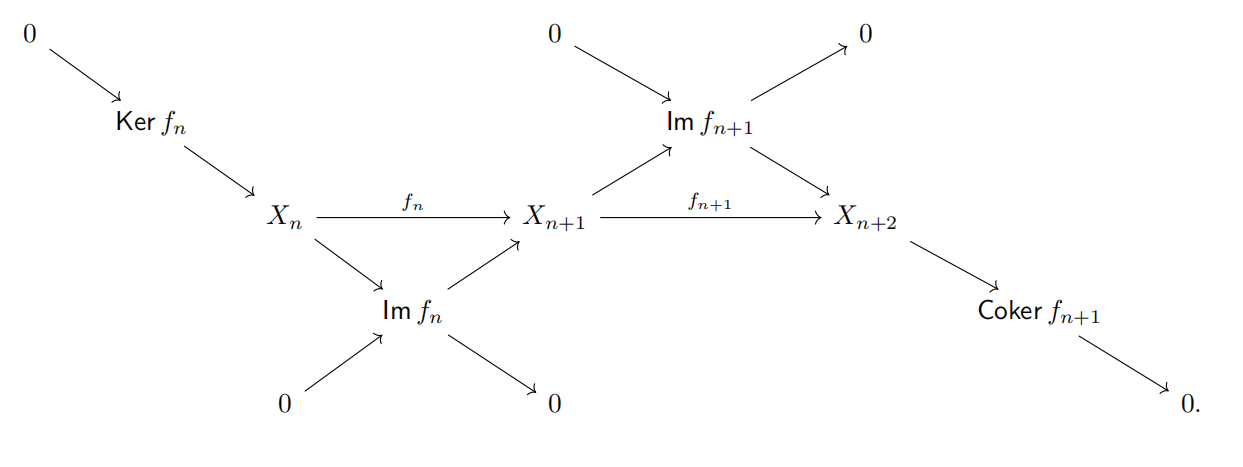
\includegraphics[width=15cm]{1.png}
%    \caption{An image of a galaxy}
    \label{fig:1}
\end{figure}

The diagonals are exact. (Proving this is a straightforward exercise.) The image of this diagram in $\mathscr{D}$ :
\begin{figure}[htp]
    \centering
    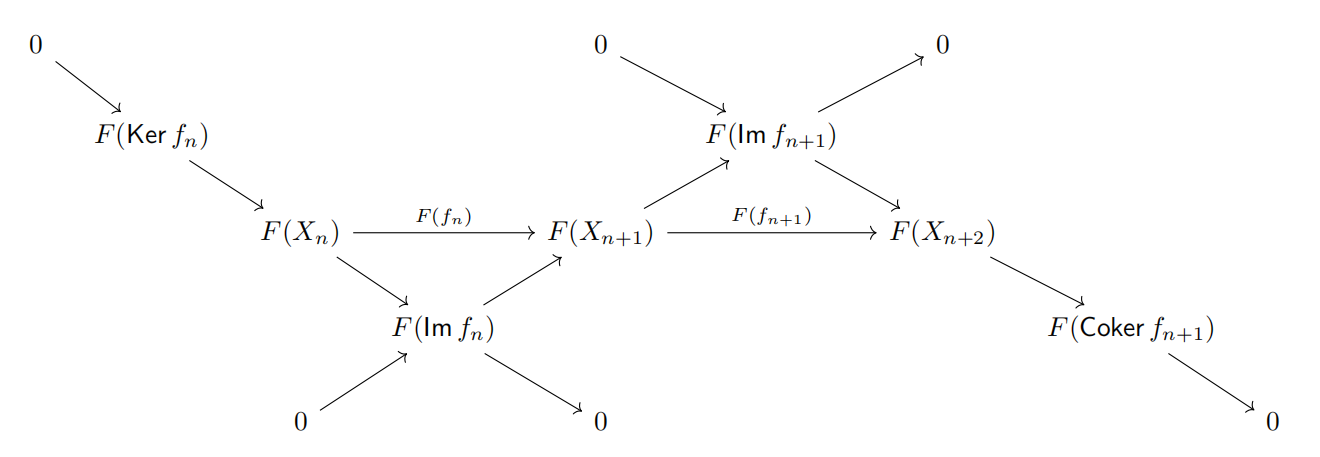
\includegraphics[width=15cm]{2.png}
    \label{fig:2}
\end{figure}

also has exact diagonals. (Here we used the fact that $F(0) \cong 0$)

We can compute
$$
\operatorname{Im} F\left(f_{n}\right)=\operatorname{Im}\left(F\left(X_{n}\right) \rightarrow F\left(\operatorname{Im} f_{n}\right) \rightarrow F\left(X_{n+1}\right)\right)=\operatorname{Im}\left(F\left(\operatorname{Im} f_{n}\right) \rightarrow F\left(X_{n+1}\right)\right)
$$

since $F\left(X_{n}\right) \rightarrow F\left(\operatorname{Im} f_{n}\right)$ is epic. Also
$$
\operatorname{Im}\left(F\left(\operatorname{Im} f_{n}\right) \rightarrow F\left(X_{n+1}\right)\right)=\operatorname{Ker}\left(F\left(X_{n+1}\right) \rightarrow F\left(\operatorname{Im} f_{n+1}\right)\right)=\operatorname{Ker}\left(F\left(X_{n+1}\right) \rightarrow F\left(\operatorname{Im} f_{n+1}\right) \rightarrow F\left(X_{n+2}\right)\right)
$$

since $F(\operatorname{Im} g) \rightarrow F\left(X_{n+2}\right)$ is monic. Thus, $\operatorname{Im} F\left(f_{n}\right)=\operatorname{Ker} F\left(f_{n+1}\right)$.
\end{Proof}


\begin{remark}
    Suppose $A$ is a ring, $S \subset A$ is a multiplicative subset, and $M$ is an $A$-module.
\\   
(a) Localization of $A$-modules $Mod_A \rightarrow Mod_{S^{-1}A}$ is an exact covariant
functor
\\
(b) $(\cdot) \otimes_A M$ is a right-exact covariant functor $Mod_A \rightarrow Mod_A$. (This is a repeat of Exercise 1.3.H.)
\\
(c) $Hom(M, \cdot)$ is a left-exact covariant functor $Mod_A \rightarrow Mod_A$ 

If $\mathscr C$ is any abelian category, and $C \in\mathscr C$ , then $Hom(C, \cdot)$ is a left-exact covariant
functor $\mathscr C \rightarrow Ab$
\\
(d) $Hom(\cdot,M)$ is a left-exact contravariant functor $Mod_A \rightarrow Mod_A$

If $\mathscr C$ is any abelian category, and $C \in\mathscr C$ , then $Hom(\cdot, C)$ is a left-exact contravariant functor $\mathscr C \rightarrow Ab$
\label{remark 1.73}
\end{remark}

\begin{example}\label{example 1.75}
Suppose $M$ is a \textbf{finitely presented $A$-module}: $M$ has a finite
number of generators, and with these generators it has a finite number of relations;
or usefully equivalently, fits in an exact sequence
\begin{equation*}
    A^{\oplus q}
    \rightarrow A^{\oplus q}
    \rightarrow M
    \rightarrow 0
\end{equation*}
We can use this exact sequence and the left-exactness of $Hom$ to describe an isomorphism
\begin{equation*}
S^{-1} Hom_A(M, N) \cong Hom_{S^{-1}A}(S^{-1}M, S^{-1}N)
\end{equation*}
\end{example}
\begin{Proof}
From 
\begin{equation*}
    A^{\oplus q}\rightarrow A^{\oplus q}\rightarrow M
    \rightarrow 0
\end{equation*}

We get 
\begin{equation*}    
0
\rightarrow
Hom_A(M,N)
\rightarrow 
Hom_A(A^{\oplus q},N)
\rightarrow 
Hom_A(A^{\oplus q},N)
\end{equation*}
\begin{equation*}    
0
\rightarrow
S^{-1}Hom_A(M,N)
\rightarrow 
S^{-1}Hom_A(A^{\oplus q},N)
\rightarrow 
S^{-1}Hom_A(A^{\oplus q},N)
\end{equation*}

and
\begin{equation*}    S^{-1}A^{\oplus q}
\rightarrow S^{-1}A^{\oplus q}
\rightarrow 
S^{-1}M
\rightarrow
0
\end{equation*}
\begin{equation*}    
0
\rightarrow
Hom_{S^{-1}A}(S^{-1}M,S^{-1}N)
\rightarrow 
Hom_{S^{-1}A}(S^{-1}A^{\oplus q},S^{-1}N)
\rightarrow
Hom_{S^{-1}A}(S^{-1}A^{\oplus q},S^{-1}N)
\end{equation*}

So we just need to consider $M=A^{\oplus k}$

We know 
\begin{equation*}
  Hom_A(A^{\oplus k},N)\cong (Hom_A(A,N))^{\oplus k},\;Hom_A(A,N)\cong N
\end{equation*}

So
\begin{equation*} S^{-1}Hom_A(A^{\oplus k},N)
\cong
S^{-1}(N^{\oplus k})
\cong
Hom_{S^{-1}A}(S^{-1}A^{\oplus k}, S^{-1}N)
\end{equation*}
\begin{equation*}
\frac{(n_1,\cdots,n_k)}{s}
\mapsto
(\frac{(a_1,\cdots,a_k)}{s}
\mapsto
\frac{a_1n_1+\cdots+a_kn_k}{s})
\end{equation*}
\end{Proof}

\begin{example}
Hom doesn’t always commute with localization :

In the language of Example\ref{example 1.75}, take $A = N = \mathbb Z$, $M =\mathbb Q$, and $S =\mathbb Z \setminus \left\{0\right\}$
\begin{equation*}
S^{-1} Hom_A(M, N) = S^{-1}0=0,
Hom_{S^{-1}A}(S^{-1}M, \;\;
S^{-1}N)=Hom_\mathbb Q(\mathbb Q,\mathbb Q)=\mathbb Q
\end{equation*}
\end{example}

\begin{remark}
\textbf{Interaction of homology and (right/left-)exact functors}

Suppose $F:\mathscr A \rightarrow \mathscr B$ is a
covariant functor of abelian categories, and $ C
^\bullet$
is a complex in $\mathscr A$

(a) (F right-exact yields $\mathrm{FH}^{\bullet} \longrightarrow \mathrm{H}^{\bullet} \mathrm{F}$ ) If $\mathrm{F}$ is right-exact, describe a natural morphism $\mathrm{FH}^{\bullet} \rightarrow \mathrm{H}^{\bullet} \mathrm{F}$. (More precisely, for each $i$, the left side is $\mathrm{F}$ applied to the cohomology at piece $i$ of $\mathrm{C}^{\bullet}$, while the right side is the cohomology at piece $i$ of $\mathrm{FC}^{\bullet}$.)

(b) (F left-exact yields $\mathrm{FH}^{\bullet} \longleftarrow \mathrm{H}^{\bullet} \mathrm{F}$ ) If $\mathrm{F}$ is left-exact, describe a natural morphism $\mathrm{H}^{\bullet} \mathrm{F} \rightarrow \mathrm{FH}^{\bullet}$.

(c) ( $\mathrm{F}$ exact yields $\mathrm{FH}^{\bullet} \stackrel{\sim}{\longleftrightarrow} \mathrm{H}^{\bullet} \mathrm{F}$ ) If $\mathrm{F}$ is exact, show that the morphisms of (a) and (b) are inverses and thus isomorphisms.
\end{remark}

Hint for (a): use $\mathrm{C}^{i} \stackrel{d^{i}}{\longrightarrow} \mathrm{C}^{i+1} \longrightarrow$ coker $d^{i} \longrightarrow 0$ to give an isomorphism $F\, coker\, d^{i} \cong\, coker\,F\, d^{i}$. Then use the first line of (\ref{equation 1.5.4}) to give a epimorphism $\mathrm{F\,im} \mathrm{d}^{i} \longrightarrow \mathrm{im}\, \mathrm{Fd}^{i}$. Then use the second line of (\ref{equation 1.5.4}) to give the desired map $\mathrm{FH}^{i} \mathrm{C}^{\bullet} \longrightarrow \mathrm{H}^{i} \mathrm{FC}^\bullet$. While you are at it, you may as well describe a map for the fourth member of the quartet \{coker, im, H, ker\}: $\operatorname{F\,ker d^{i}} \longrightarrow \operatorname{ker\,Fd}^{i}$

\begin{remark}
If this makes your head spin, you may prefer to think of it in the following specific case, where both $\mathscr{A}$ and $\mathscr{B}$ are the category of A-modules, and $\mathrm{F}$ is $(\cdot) \otimes \mathrm{N}$ for some fixed $\mathrm{N}$-module. Your argument in this case will translate without change to yield a solution to Remark \ref{remark 1.73}(a) and (c) in general. If $\otimes N$ is exact, then $N$ is called a flat A-module.

For example, localization is exact (Remark \ref{remark 1.73}), so $S^{-1} A$ is a flat A-algebra for all multiplicative sets $S$\,($S^{-1}M\cong M\otimes_A S^{-1}A$). Thus taking cohomology of a complex of $A$-modules commutes with localization
\end{remark} 
\begin{remark}
\textbf{Interaction of adjoints, (co)limits, and (left- and right-) exactness}

A surprising number of arguments boil down to the statement:

Limits commute with limits and right adjoints. In particular, in an abelian category, because kernels are limits, both right adjoints and limits are left-exact.

as well as its dual:

Colimits commute with colimits and left adjoints. In particular, because cokernels are colimits, both left adjoints and colimits are right-exact.

The latter has a useful extension:

In $\operatorname{Mod}_{A}$, colimits over filtered index categories are exact.
\end{remark}
\begin{remark}
$\star \star$ Caution. It is not true that in abelian categories in general, colimits over filtered index categories are exact. %(Grothendieck realized the desirability of such colimits being exact, and formalized this as his "AB5" axiom, see for example [Stacks, tag 079A].) Here is a counterexample. Because the axioms of abelian categories are self-dual, it suffices to give an example in which a filtered limit fails to be exact, and we do this. 

Fix a prime $p$. In the category $A b$ of abelian groups, for each positive integer $n$, we have an exact sequence $\mathbb{Z} \rightarrow \mathbb{Z} /\left(p^{n}\right) \rightarrow 0$. Taking the limit over all $n$ in the obvious way, we obtain $\mathbb{Z} \rightarrow \mathbb{Z}_{p} \rightarrow 0$, which is certainly not exact.)

%See Unimportant Remark \ref{remark 1.73} for another dashed hope.
\end{remark}
\begin{theorem}
(\textbf{kernels commute with limits})

Suppose $\mathscr{C}$ is an abelian category, and a: $\mathscr{I} \rightarrow \mathscr{C}$ and b: $\mathscr{I} \rightarrow \mathscr{C}$ are two diagrams in $\mathscr{C}$ indexed by $\mathscr{I}$. For convenience, let $A_{i}=a(i)$ and $B_{i}=b(i)$ be the objects in those two diagrams. Let $h_{i}: A_{i} \rightarrow B_{i}$ be maps commuting with the maps in the diagram. 

(Translation:
$h$ is a natural transformation of functors $a \rightarrow b$) Then the $ker\, h_i$
form another diagram in $\mathscr{C}$ indexed by $\mathscr{I}$. Describe a canonical isomorphism
 $\lim \limits_{\longleftarrow} \operatorname{ker} h_{i} \cong \operatorname{ker}\left(\lim \limits_{\longleftarrow}A_{i} \rightarrow \lim \limits_{\longleftarrow} B_{i}\right)$, assuming the limits exist.
\end{theorem}
\begin{Proof}
    \begin{figure}[htp]
    \centering
    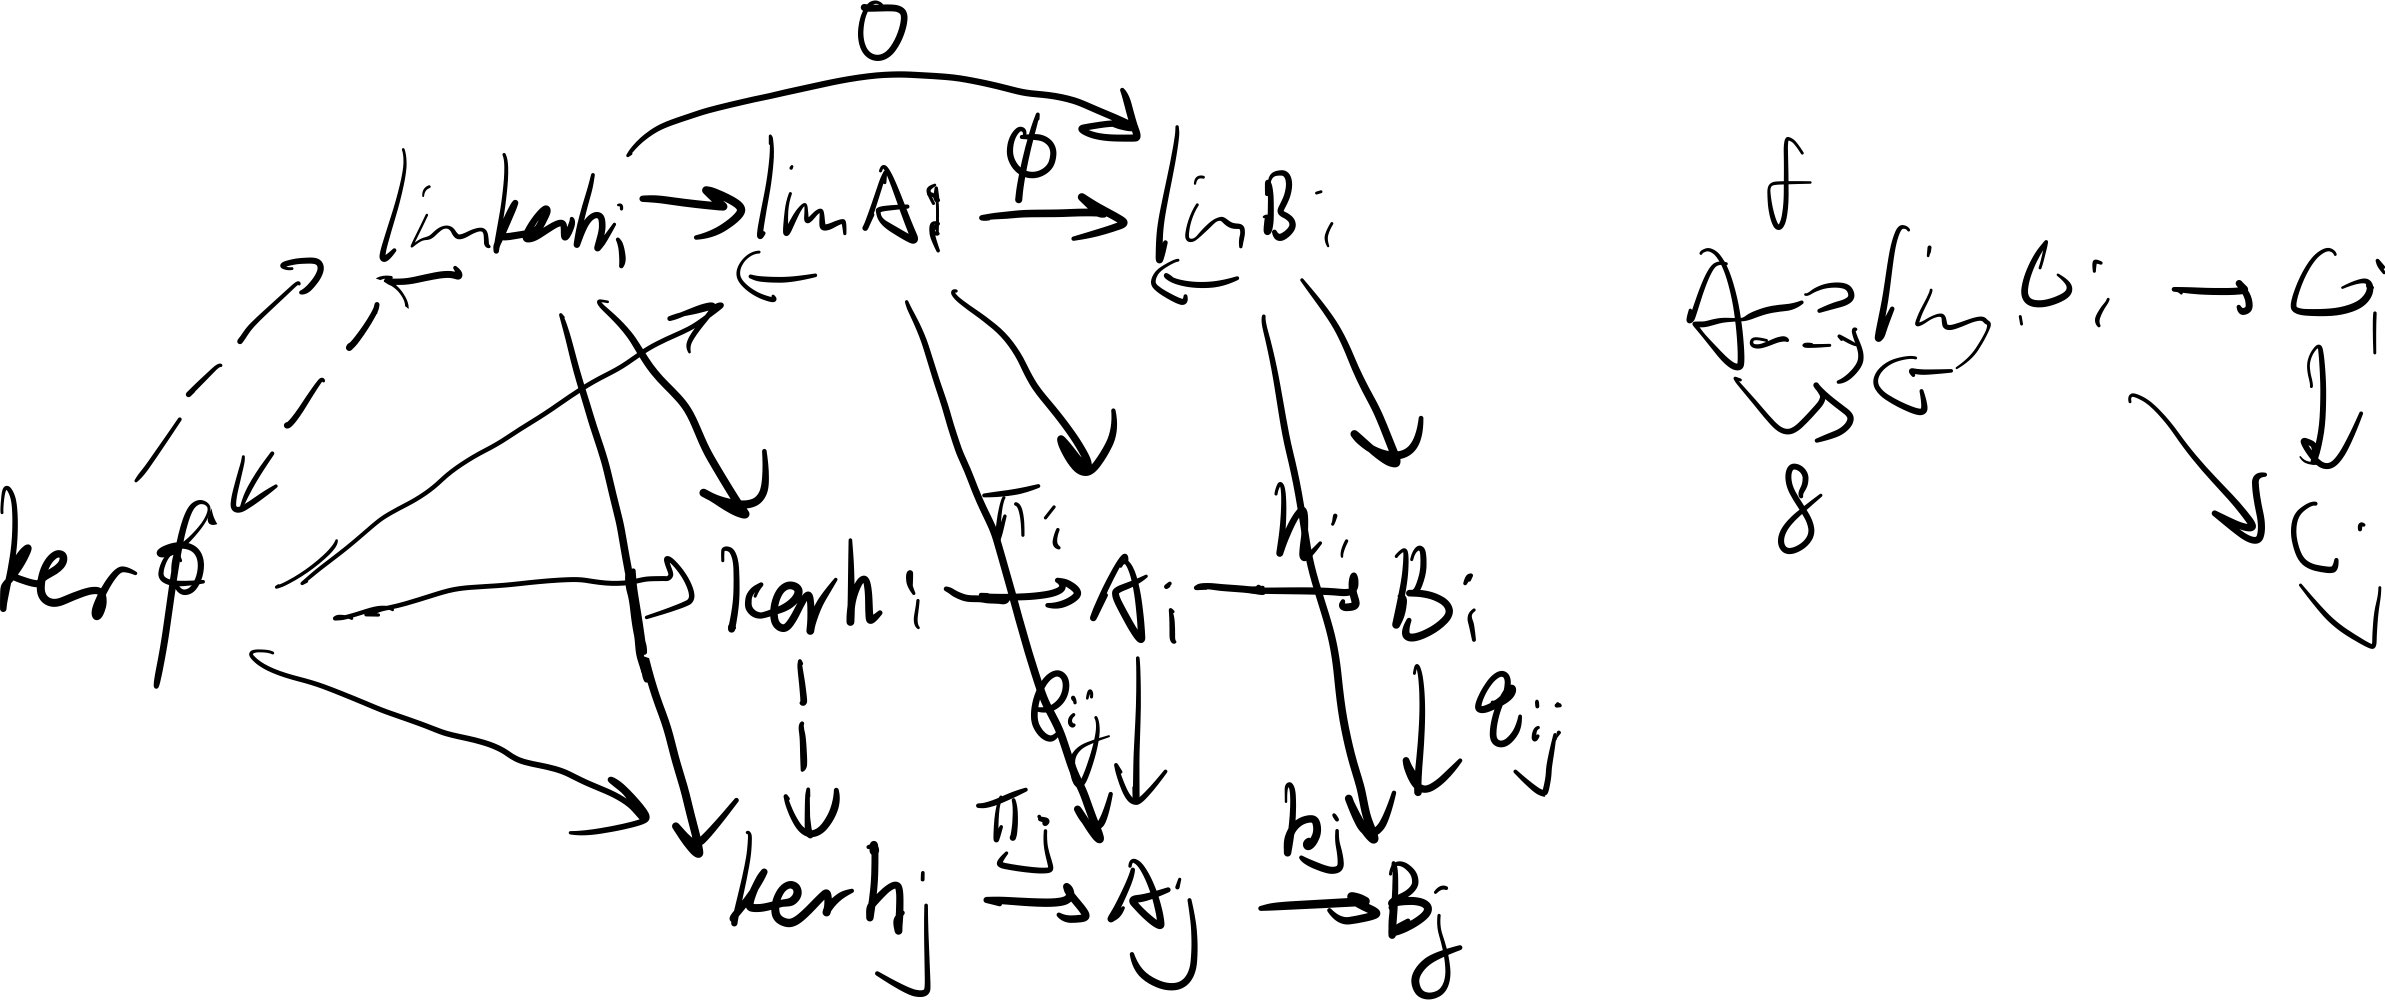
\includegraphics[width=10cm]{3.png}
    \label{fig:3}
\end{figure}

\end{Proof}
\begin{theorem}
(\textbf{Limits commute with limits})

Let $F: I \times J \rightarrow C$ be a functor. If ${\lim \limits_{\longleftarrow}} _j F(i, j)$ exists for all $i \in I$ then we find that ${\lim \limits_{\longleftarrow}} _i {\lim \limits_{\longleftarrow}} _j F(i, j)$ exists iff ${\lim \limits_{\longleftarrow}} _{(i, j)} F(i, j)$ exists, in which case they are canonically isomorphic.

In particular
$$
{\lim \limits_{\longleftarrow}} _i {\lim \limits_{\longleftarrow}} _j F(i, j) \cong {\lim \limits_{\longleftarrow}} _j {\lim \limits_{\longleftarrow}} _i F(i, j)
$$

if both sides exist.

I should briefly clarify what ${\lim \limits_{\longleftarrow}} _i {\lim \limits_{\longleftarrow}} _j F(i, j)$ actually means. A morphism $f: i \rightarrow i^{\prime}$ induces a natural transformation $F(i,-) \Rightarrow F\left(i^{\prime},-\right)$, which induces a morphism ${\lim \limits_{\longleftarrow}} _j F(f, j): {\lim \limits_{\longleftarrow}} _j F(i, j) \rightarrow {\lim \limits_{\longleftarrow}} _j F\left(i^{\prime}, j\right)$. So the $\operatorname{limits}_j {\lim \limits_{\longleftarrow}} _j F(i, j)$ in fact assemble into a functor $I \rightarrow C$, and ${\lim \limits_{\longleftarrow}} _i {\lim \limits_{\longleftarrow}} _j F(i, j)$ is the limit of this functor.
\end{theorem}
\begin{Proof}
    \begin{figure}[htp]
    \centering
    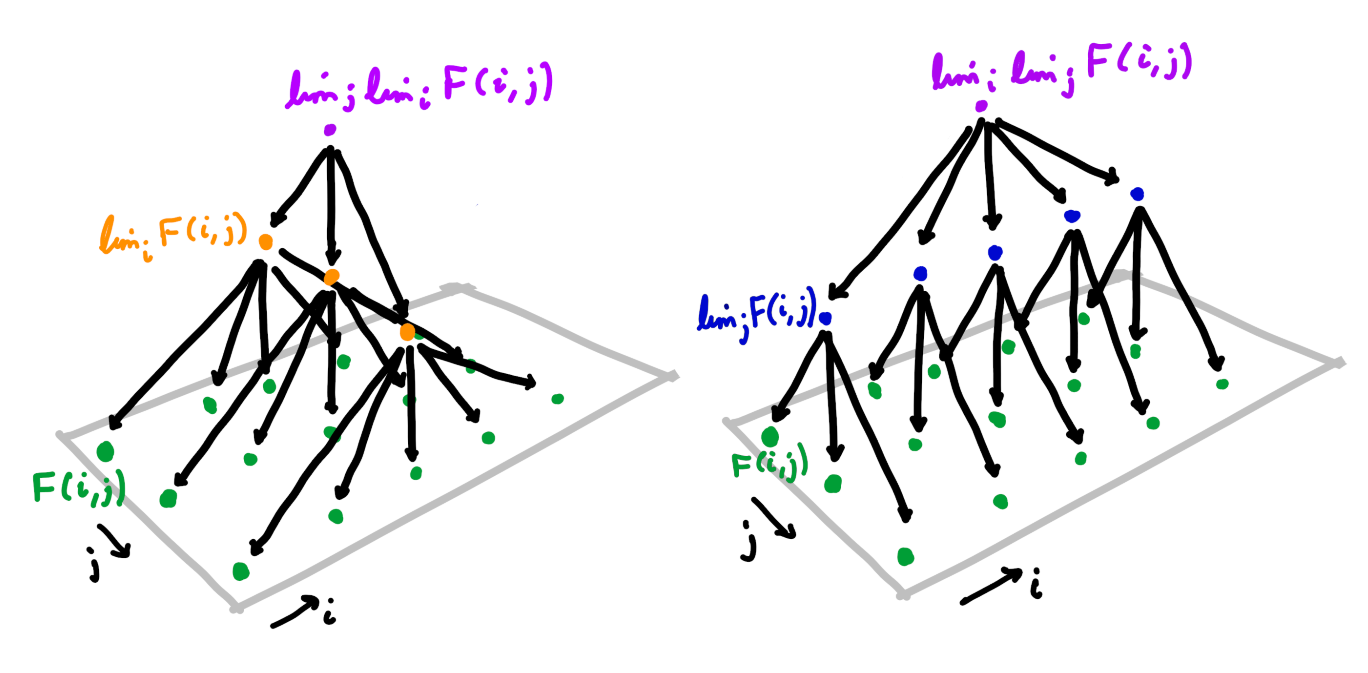
\includegraphics[width=9cm]{4.png}
    \label{fig:4}
    \end{figure}
    
\end{Proof}
\begin{theorem}
(\textbf{right adjoints commute with limits})

Suppose (F: $\mathscr{C} \rightarrow$ $\mathscr{D}, \mathrm{G}: \mathscr{D} \rightarrow \mathscr{C})$ is a pair of adjoint functors. If $\mathrm{A}={\lim \limits_{\longleftarrow}} _{i} \mathrm{~A}_{i}$ is a limit in $\mathscr{D}$ of a diagram indexed by $\mathscr{I}$, then $\mathrm{GA}={\lim \limits_{\longleftarrow}} _{\mathfrak{G}} \mathrm{GA}_{i}$ (with the corresponding maps $\mathrm{GA} \rightarrow \mathrm{GA}_{i}$ ) is a limit in $\mathscr{C}$.
\end{theorem}
\begin{Proof}
    We must show that $\mathrm{GA} \rightarrow \mathrm{GA}_{i}$ satisfies the universal property of limits. Suppose we have maps $W \rightarrow \mathrm{GA}_{i}$ commuting with the maps of $\mathscr{I}$. We wish to show that there exists a unique $W \rightarrow G A$ extending the $W \rightarrow G A_{i}$. By adjointness of $F$ and G, we can restate this as: Suppose we have maps FW $\rightarrow A_{i}$ commuting with the maps of $\mathscr{I}$. We wish to show that there exists a unique $\mathrm{FW} \rightarrow$ A extending the $\mathrm{FW} \rightarrow \mathrm{A}_{i}$. But this is precisely the universal property of the limit.
\end{Proof}
\begin{corollary}
If $F$ and $G$ are additive functors between abelian categories, and $(F, G)$ is an
adjoint pair, then (as kernels are limits and cokernels are colimits) $G$ is left-exact
and $F$ is right-exact
\end{corollary}
\begin{example}
    In $Mod_{A}$, colimits over filtered index categories are exact. (Your argument will apply without change to any abelian category whose objects can be interpreted as "sets with additional structure".) Right-exactness follows from the above discussion, so the issue is left-exactness. 

     (Possible hint:
After you show that localization is exact, or stalkification is exact, in a hands-on way, you will be easily able to prove this)
\end{example}
\begin{example}
    Filtered colimits commute with homology in $\operatorname{Mod}_{A}$
    
    Hint: use the FHHF Theorem, and the previous Exercise
\end{example}
\begin{remark}
    Suppose
    \[\begin{tikzcd}
	& \vdots & \vdots & \vdots \\
	0 & {A_{n+1}} & {B_{n+1}} & {C_{n+1}} & 0 \\
	0 & {A_{n}} & {B_{n}} & {C_{n}} & 0 \\
	& \vdots & \vdots & \vdots \\
	0 & {A_{0}} & {B_{0}} & {C_{0}} & 0 \\
	& 0 & 0 & 0
	\arrow[from=1-2, to=2-2]
	\arrow[from=2-2, to=3-2]
	\arrow[from=3-2, to=4-2]
	\arrow[from=4-2, to=5-2]
	\arrow[from=5-2, to=6-2]
	\arrow[from=5-1, to=5-2]
	\arrow[from=2-2, to=2-3]
	\arrow[from=2-1, to=2-2]
	\arrow[from=3-1, to=3-2]
	\arrow[from=5-2, to=5-3]
	\arrow[from=3-3, to=4-3]
	\arrow[from=4-3, to=5-3]
	\arrow[from=3-2, to=3-3]
	\arrow[from=1-3, to=2-3]
	\arrow[from=2-3, to=3-3]
	\arrow[from=5-3, to=6-3]
	\arrow[from=2-3, to=2-4]
	\arrow[from=3-3, to=3-4]
	\arrow[from=2-4, to=3-4]
	\arrow[from=1-4, to=2-4]
	\arrow[from=2-4, to=2-5]
	\arrow[from=3-4, to=3-5]
	\arrow[from=5-3, to=5-4]
	\arrow[from=3-4, to=4-4]
	\arrow[from=4-4, to=5-4]
	\arrow[from=5-4, to=5-5]
	\arrow[from=5-4, to=6-4]
\end{tikzcd}\]
    
    is an inverse system of exact sequences of modules over a ring, such that the maps $A_{n+1} \rightarrow A_{n}$ are surjective. (We say: "transition maps of the left term are surjective".) 
    
    Then the limit

$$
0 \longrightarrow \lim _{\longleftarrow} A_{n} \longrightarrow \lim _{\longleftarrow} B_{n} \longrightarrow \lim _{\longleftarrow} C_{n} \longrightarrow 0
$$

is also exact. (You will need to define the maps in)
\end{remark}
\begin{remark}
Based on these ideas, you may suspect that rightexact functors always commute with colimits. The fact that tensor product commutes with infinite direct sums may reinforce this idea. Unfortunately, it is not true - "double dual" $\cdot^{\vee \vee} : Vec_{k} \rightarrow Vec_{k}$ is covariant and right exact (why is it right-exact?), but does not commute with infinite direct sums, as $\prod_{i=1}^{\infty}\left(k^{\vee \vee}\right)$ is not isomorphic to $\left(\prod_{i=1}^{\infty} k\right)^{\vee \vee}$.
\end{remark}




\newpage
\section{Sheaves}
\subsection{Sheaf and presheaf}
\begin{definition}
\textbf{Presheaves}

Presheaves are a way of keeping track of algebraic data on a topological space. More precisely:

Let $X$ be a topological space and $\mathcal{C}$ a category. A presheaf $\mathcal{F}$ of $\mathcal{C}$ on $X$ consists of

(1) For all $U \subseteq X$ open, an object $\mathcal{F}(U)$ in $\mathcal{C}$.

(2) For all $V \subseteq U \subseteq X$ open, a morphism $\rho_{U V}: \mathcal{F}(U) \rightarrow \mathcal{F}(V)$ in $\mathcal{C}$ such that

(i) For all $U \subseteq X$ open, $\rho_{U U}: \mathcal{F}(U) \rightarrow \mathcal{F}(U)$ is the identity.

(ii) For all $W \subseteq V \subseteq U \subseteq X$ open, we have $\rho_{U W}=\rho_{V W} \circ \rho_{U V}$, that is, the following diagram commutes:
\begin{center}

\tikzset{every picture/.style={line width=0.75pt}} %set default line width to 0.75pt        

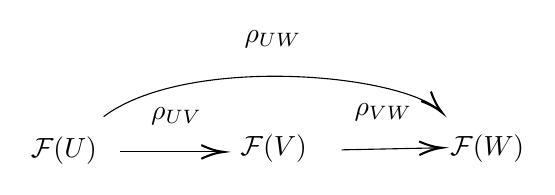
\begin{tikzpicture}[x=0.75pt,y=0.75pt,yscale=-1,xscale=1]
%uncomment if require: \path (0,872); %set diagram left start at 0, and has height of 872

%Straight Lines [id:da25009039005578937] 
\draw    (142.33,83) -- (190.33,83) ;
\draw [shift={(192.33,83)}, rotate = 180] [color={rgb, 255:red, 0; green, 0; blue, 0 }  ][line width=0.75]    (10.93,-3.29) .. controls (6.95,-1.4) and (3.31,-0.3) .. (0,0) .. controls (3.31,0.3) and (6.95,1.4) .. (10.93,3.29)   ;
%Straight Lines [id:da7919347492895541] 
\draw    (249,82) -- (295.33,81.04) ;
\draw [shift={(297.33,81)}, rotate = 178.81] [color={rgb, 255:red, 0; green, 0; blue, 0 }  ][line width=0.75]    (10.93,-3.29) .. controls (6.95,-1.4) and (3.31,-0.3) .. (0,0) .. controls (3.31,0.3) and (6.95,1.4) .. (10.93,3.29)   ;
%Curve Lines [id:da21644996179503995] 
\draw    (134.33,66) .. controls (173.53,36.6) and (274.52,44.66) .. (296.11,62.87) ;
\draw [shift={(297.33,64)}, rotate = 225.51] [color={rgb, 255:red, 0; green, 0; blue, 0 }  ][line width=0.75]    (10.93,-3.29) .. controls (6.95,-1.4) and (3.31,-0.3) .. (0,0) .. controls (3.31,0.3) and (6.95,1.4) .. (10.93,3.29)   ;

% Text Node
\draw (156,60.4) node [anchor=north west][inner sep=0.75pt]    {$\rho _{UV}$};
% Text Node
\draw (254,58.4) node [anchor=north west][inner sep=0.75pt]    {$\rho _{VW}$};
% Text Node
\draw (201,23.4) node [anchor=north west][inner sep=0.75pt]    {$\rho _{UW}$};
% Text Node
\draw (98,74.4) node [anchor=north west][inner sep=0.75pt]    {$\mathcal{F}( U)$};
% Text Node
\draw (199,73.4) node [anchor=north west][inner sep=0.75pt]    {$\mathcal{F}( V)$};
% Text Node
\draw (300,73.4) node [anchor=north west][inner sep=0.75pt]    {$\mathcal{F}( W)$};


\end{tikzpicture}

\end{center}

$\quad$ Elements $s \in \mathcal{F}(U)$ are called \textbf{sections} of $\mathcal{F}$ over $U$. The object $\mathcal{F}(U)$ is called space of sections of $\mathcal{F}$ over $U$.

- Elements $s \in \mathcal{F}(X)$ are called \textbf{global sections} of $\mathcal{F}$. The object $\mathcal{F}(X)$ is called space of global sections of $\mathcal{F}$.

- Alternative notations for $\mathcal{F}(U)$ are $\Gamma(U, \mathcal{F})$ and $H^{0}(U, \mathcal{F})$.

- The morphisms $\rho_{U V}$ are called \textbf{restriction maps}. For $V \subseteq U$ open and $s \in \mathcal{F}(U)$, we will sometimes write $\left.s\right|_{V}$ for $\rho_{U V}(s)$ and call $\left.s\right|_{V}$ the \textbf{restriction} of $s$ (from $U$ to $V$ ).
\end{definition}
\begin{example}
Let $X$ be a topological space.

(1) For any object $A$ in a category $\mathcal{C}$, the \textbf{constant presheaf} with value $A$ is the presheaf $A^{\prime}$ with $\underline{A}^{\prime}(U)=A$ and $\rho_{U V}=\operatorname{id}_{A}$ for all $V \subseteq U \subseteq X$ open.

(2) The \textbf{presheaf of continuous functions} on $X$ is defined by setting $\mathcal{C}^{0}(U):=C^{0}(U):=\{f$ : $U \rightarrow \mathbb{R} \mid f$ continuous $\}$ and $\rho_{U V}: \mathcal{C}^{0}(U) \rightarrow \mathcal{C}^{0}(V),\left.f \mapsto f\right|_{V}$. This can be considered as a presheaf of sets, abelian groups, or even rings.

(3) More generally, if $\pi: Y \rightarrow X$ is a continuous map of topological spaces, we can look at the presheaf (of sets) of continuous sections of $\pi$ defined as $\mathcal{F}_{\pi}(U):=\{s: U \rightarrow Y \mid$ $s$ continuous, $\left.\pi \circ s=\mathrm{id}_{U}\right\}$ with $\rho_{U V}$ the obvious restriction maps.
\end{example}

\begin{remark}
Let $X$ be a topological space and let $\operatorname{Ouv}_{X}$ be the category of open subsets of $X$, that is, the category with:

- Objects: $U \subseteq X$ open

- Morphisms:

$$
\operatorname{Hom}(U, V)=\left\{\begin{array}{l}
\emptyset \text { if } U \nsubseteq V \\
\iota \text { if } U \subseteq V \text { where } \iota \text { denotes the inclusion }
\end{array}\right.
$$

Then, a presheaf on $X$ with values in a category $\mathcal{C}$ is the same as a contravariant functor from $\operatorname{Ouv}_{X}$ to $\mathcal{C}$.
\end{remark}


\begin{definition}
The \textbf{germ} of a differentiable function. Before we do, we first give another definition, that of the germ of a differentiable function at a point $p \in X$. Intuitively, it is a "shred" of a differentiable function at $p$. Germs are objects of the form $\{(f$, open $U): p \in U, f \in \mathscr{O}(U)\}$ modulo the relation that $(f, U) \sim(g, V)$ if there is some open set $W \subset U, V$ containing $p$ where $\left.f\right|_{W}=\left.g\right|_{W}$ (i.e., $res_{U, W} f= res _{V, W} g$ ). In other words, two functions that are the same in an open neighborhood of $p$ (but may differ elsewhere) have the same germ. We call this set of germs the \textbf{stalk} at $p$, and denote it $\mathscr{O}_{p}$. Notice that the stalk is a ring: you can add two germs, and get another germ: if you have a function $f$ defined on $U$, and a function $g$ defined on $V$, then $f+g$ is defined on $U \cap V$. Moreover, $f+g$ is well-defined: if $\tilde{f}$ has the same germ as $f$, meaning that there is some open set $W$ containing $p$ on which they agree, and $\tilde{g}$ has the same germ as $g$, meaning they agree on some open $W^{\prime}$ containing $p$, then $\tilde{f}+\tilde{g}$ is the same function as $f+g$ on $U \cap V \cap W \cap W^{\prime}$.

Notice also that if $\mathrm{p} \in \mathrm{U}$, you get a map $\mathscr{O}(\mathrm{U}) \rightarrow \mathscr{O}_{\mathrm{p}}$. Experts may already see that we are talking about germs as colimits.

We can see that $\mathscr{O}_{\mathrm{p}}$ is a local ring as follows. Consider those germs vanishing at $p$, which we denote $\mathfrak{m}_{\mathfrak{p}} \subset \mathscr{O}_{\mathfrak{p}}$. They certainly form an ideal: $\mathfrak{m}_{\mathfrak{p}}$ is closed under addition, and when you multiply something vanishing at $p$ by any function, the result also vanishes at $p$. We check that this ideal is maximal by showing that the quotient ring is a field:

$$
0 \longrightarrow \mathfrak{m}_{\mathfrak{p}}:=\text { ideal of germs vanishing at } \mathrm{p} \longrightarrow \mathscr{O}_{\mathfrak{p}} \stackrel{f \mapsto f(p)}{\longrightarrow} \mathbb{R} \longrightarrow 0
$$
\end{definition}
\begin{definition}
    \textbf{germ},
    \textbf{stalk}

    Define the stalk of a presheaf $\mathcal{F}$ at a point $p$ to be the set of germs of $\mathcal{F}$ at $p$, denoted $\mathcal{F}_{p}$, as in the example above. Germs correspond to sections over some open set containing $p$, and two of these sections are considered the same if they agree on some smaller open set. More precisely: the stalk is
$$
\{(\text { open } \mathrm{U},\mathrm{f}): \mathrm{p} \in \mathrm{U}, \mathrm{f} \in \mathcal{F}(\mathrm{U})\}
$$

modulo the relation that $(U,f) \sim(V,g)$ if there is some open set $W \subset U, V$ where $p \in W$ and $\operatorname{res}_{U, W} f=$ res $_{V, W} g$. Write $\overline{(U,f)}$ for the equivalence class of $(U,f)$ in the stalk

A useful equivalent definition of a \textbf{stalk} is as a colimit of all $\mathcal{F}(\mathrm{U})$ over all open sets $\mathrm{U}$ containing $\mathrm{p}$ :
$$
\mathcal{F}_{\mathrm{p}}={\lim _{\longrightarrow} }_{p\in U}\mathcal{F}(\mathrm{U}) .
$$

(The index category is a filtered set (given any two such open sets, there is a third such set contained in both))

Gien $s\in{\mathcal{F}}(U)$ and $x\in U\subseteq X,$ then we define the \textbf{the germ of} $s$ \textbf{at} $x$ to be the image of $s$ in $\mathcal{F}_{p}$ : $s_{x}=\overline{{{(U,s)}}}\in$  ${\mathcal{F}}_{x}$ 
If $\mathcal B$ is a basis for topology on $X$  then we can rewrite the stalk as
$$
{\mathcal{F}}_{x}\cong\
{\lim _{\longrightarrow} }_{ x\in U,U\in{\mathcal{B}}}\ {\mathcal{F}}(U), 
$$
\end{definition}
\begin{definition}
\textbf{Sheaf}

A presheaf is a sheaf if it satisfies two more axioms. Notice that these axioms use the additional information of when some open sets cover another.

\textbf{Identity axiom}. If $\left\{\mathrm{U}_{i}\right\}_{i \in I}$ is an open cover of $U$, and $f_{1}, f_{2} \in \mathcal{F}(U)$, and $res_{U, U_{i}} f_{1}=$ $res_{U, U_{i}} f_{2}$ for all $i$, then $f_{1}=f_{2}$.

(A presheaf satisfying the identity axiom is called a separated presheaf, but we will not use that notation in any essential way.)

\textbf{Gluability axiom}. If $\left\{\mathrm{U}_{i}\right\}_{i \in \mathrm{I}}$ is an open cover of $\mathrm{U}$, then given $\mathrm{f}_{i} \in \mathcal{F}\left(\mathrm{U}_{i}\right)$ for all $i$, such that $res_{U_{i}, U_{i} \cap U_{j}} f_{i}=res_{U_{j}, U_{i} \cap U_{j}} f_{j}$ for all $i, j$, then there is some $f \in \mathcal{F}(U)$ such that $res_{U, U_{i}} f=f_{i}$ for all $i$.

(In this case, identity means there is at most one way to glue, and gluability
means that there is at least one way to glue)

The stalk of a sheaf at a point is just its stalk as a presheaf - the same definition applies - and similarly for the germs of a section of a sheaf.
\label{def 2.6}
\end{definition}
\begin{remark}
    Interpretation in terms of the equaliser exact sequence. The two axioms for a presheaf to be a sheaf can be interpreted as "exactness" of the "equalizer exact sequence": $$\cdot\longrightarrow \mathcal{F}(\mathrm{U}) \longrightarrow \prod \mathcal{F}\left(\mathrm{U}_{\mathrm{i}}\right) \rightrightarrows \prod \mathcal{F}\left(\mathrm{U}_{\mathrm{i}} \cap \mathrm{U}_{\mathrm{j}}\right)$$
    
    Identity is exactness at $\mathcal{F}(\mathrm{U})$, and gluability is exactness at $\prod \mathcal{F}\left(\mathrm{U}_{\mathrm{i}}\right)$.
\end{remark}
\begin{example}
Let $X$ be a topological space.

(1) 
(An additional axiom sometimes included is that $\mathcal{F}(\varnothing)$ is a one-element set, and in general, for a sheaf with values in a category, $\mathcal{F}(\varnothing)$ is required to be the final object in the category. This actually follows from the above definitions, assuming that the empty product is appropriately defined as the final object.)

If $\mathcal{F}$ is a sheaf of sets (or abelian groups, rings, etc.), then, by Identity axiom of Def\ref{def 2.6} applied to $I=\emptyset$, the underlying set of $\mathcal{F}(\emptyset)$ has at most one element, and by Gluability axiom, it has at least one element.

If $\mathrm{U}$ and $\mathrm{V}$ are disjoint, then $\mathcal{F}(\mathrm{U} \cup \mathrm{V})=\mathcal{F}(\mathrm{U}) \times \mathcal{F}(\mathrm{V})$. Here we use the fact that $\mathcal{F}(\varnothing)$ is the final object.

(2) The presheaves $\mathcal{C}^{0}$ (and $\mathcal{C}^{\infty}$ if $X=\mathbb{R}^{n}$ ) on $X$ are sheaves, since:

(i) Two continuous functions $f, g$ that coincide on an open cover of $U \subseteq X$ coincide at every point, hence they are equal.

(ii) Given $U \subseteq X$ open, a cover $U=\cup_{i \in I} U_{i}$, and continuous functions $f_{i}: U_{i} \rightarrow \mathbb{R}$ that agree on $U_{i} \cap U_{j}$, the function

$$
\begin{aligned}
f: U & \rightarrow \mathbb{R} \\
x & \mapsto f_{i}(x) \text { if } x \in U_{i}
\end{aligned}
$$

is well-defined. By construction, $\left.f\right|_{U_{i}}=f_{i}$ and $f$ is continuous (resp. differentiable), since continuity (resp. differentiability) at any point can be checked on an open neighborhood.

(3)\textbf{constant sheaf }

let $\mathcal{F}(\mathrm{U})$ be the maps to $S$ that are locally constant, i.e., for any point $p$ in $\mathrm{U}$, there is an open neighborhood of $p$ where the function is constant. Show that this is a sheaf. (A better description is this: endow $\mathrm{S}$ with the discrete topology, and let $\mathcal{F}(\mathrm{U})$ be the continuous maps $\mathrm{U} \rightarrow \mathrm{S}$.) This is called the constant sheaf (associated to S); (do not confuse it with the constant presheaf) 

We denote this sheaf $\underline{S}$

(4)\textbf{morphisms glue}

Suppose $Y$ is a topological space. Show that "continuous maps to $Y$ " form a sheaf of sets on $X$. More precisely, to each open set $U$ of $X$, we associate the set of continuous maps of $U$ to $Y$. Show that this forms a sheaf. ((2), with $Y=\mathbb{R}$, and (3), with $Y=S$ with the discrete topology, are both special cases)
\end{example}
\begin{example}
    Important Example: \textbf{Restriction of a sheaf}
    
    Suppose $\mathcal{F}$ is a sheaf on $X$, and $U$ is an open subset of $X$. Define the restriction of $\mathcal{F}$ to $U$, denoted $\mathcal{F} \mid_ \mathrm{U}$, to be the collection $\mathcal{F} \mid _ \mathrm{U}(\mathrm{V})=\mathcal{F}(\mathrm{V})$ for all open subsets $V \subset \mathrm{U}$. Clearly this is a sheaf on U. 
\end{example}
\begin{example}
Important Example: the \textbf{skyscraper sheaf}

Suppose $X$ is a topological space, with $p \in X$, and $S$ is a set. Let $i_{p}: p \rightarrow X$ be the inclusion. Then $i_{p, *} S$ defined by

$$
i_{p, *} S(U)= \begin{cases}S & \text { if } p \in U, \text { and } \\ \{e\} & \text { if } p \notin U\end{cases}
$$

forms a sheaf. Here $\{e\}$ is any one-element set. This is called a skyscraper sheaf. 

(Mild caution: this informal picture suggests that the only nontrivial stalk of a skyscraper sheaf is at $p$, which isn't the case) 

There is an analogous definition for sheaves of abelian groups, except $i_{p, *}(S)(U)=\{0\}$ if $p \notin U$; and for sheaves with values in a category more generally, $i_{p, *} S(U)$ should be a final object
\end{example}
\begin{theorem}
    Let $A$ be a ring, and let the basis $\mathcal B$ of $Spec\, A$ be the one made of principle open subsets, then $\mathscr O_{Spec\,A}$ is a sheaf on $\mathcal B$.

    We have a sheaf of rings on ${Spec\,A}$ which on principal open subsets $D(f)$ is simply
$$
{\cal O}_{Spec\,A}(D(f))={\cal O}(D(f))=A[f^{-1}]. 
$$
\end{theorem}
\begin{remark}
    $\star$\;\textbf{The space of sections (espace étalé) of a (pre)sheaf}. 
    
    Suppose $\mathcal{F}$ is a presheaf (e.g., a sheaf) on a topological space $X$. Construct a topological space $F$ along with a continuous map $\pi: \mathrm{F} \rightarrow \mathrm{X}$ as follows: as a set, $\mathrm{F}$ is the disjoint union of all the stalks of $\mathcal{F}$. This naturally gives a map of sets $\pi: F \rightarrow X$. Topologize $F$ as follows. Each $s$ in $\mathcal{F}(\mathrm{U})$ determines a subset $\left\{\left(x, s_{x}\right): x \in U\right\}$ of $F$. The topology on $F$ is the weakest topology such that these subsets are open. (These subsets form a base of the topology. For each $y \in F$, there is an open neighborhood $V$ of $y$ and an open neighborhood $\mathrm{U}$ of $\pi(\mathrm{y})$ such that $\left.\pi\right|_{V}$ is a homeomorphism from $\mathrm{V}$ to $\mathrm{U}$.) The topological space F could be thought of as the space of sections of $\mathcal{F}$ (and in French is called the espace étalé of $\mathcal{F}$)
\end{remark}
\begin{definition}
     \textbf{The pushforward sheaf/direct image sheaf}
     
     Suppose $\pi: X \rightarrow Y$ is a continuous map, and $\mathcal{F}$ is a presheaf on $X$. Then define $\pi_{*} \mathcal{F}$ by $\pi_{*} \mathcal{F}(V)=\mathcal{F}\left(\pi^{-1}(V)\right)$, where $V$ is an open subset of $Y$. Show that $\pi_{*} \mathcal{F}$ is a presheaf on $\mathrm{Y}$, and is a sheaf if $\mathcal{F}$ is. This is called the \textbf{pushforward} or \textbf{direct image} of $\mathcal{F}$. More precisely, $\pi_{*} \mathcal{F}$ is called the \textbf{pushforward of} $\mathcal{F}$ \textbf{by} $\pi$.

     Once we realize that sheaves form a category, we will see that the pushforward is a functor from sheaves on $X$ to sheaves on $Y$ (see next subsection).

      \textbf{pushforward induces maps of stalks}
      
      Suppose $\pi: X \rightarrow Y$ is a continuous map, and $\mathcal{F}$ is a sheaf of sets (or rings or A-modules) on X. If $\pi(p)=q$, we can describe a natural morphism of stalks $\left(\pi_{*} \mathcal{F}\right)_{q} \rightarrow \mathcal{F}_{p}$. (Use the explicit definition of stalk using representatives, or the universal property)

      (If $\phi:{\mathcal{F}} \rightarrow{\mathcal{G}}$ is a morphism of presheavesy then for each $x\in X$ we have a well-defined induced map $\phi_{x}:{\mathcal{F}}_{x}\to{\mathcal{G}}_{x}$ defined by $\overline{(U,s)}\rightarrow\overline{(U,\phi_{U}(s))}.$ The well-definedness of this map comes from the naturality properties of morphisms of presheaves)
\end{definition}
\begin{example}
As the notation suggests, the skyscraper sheaf can be interpreted as the pushforward of the constant sheaf $\underline{S}$ on a one-point space $p$, under the inclusion morphism $i_{p}:\{p\} \rightarrow X$.
\end{example}




\newpage
\subsection{Morphisms of presheaves and sheaves}
\begin{definition}
    Let $X$ be a topological space. A \textbf{morphism} $\varphi: \mathcal{F}_{1} \rightarrow \mathcal{F}_{2}$ \textbf{of presheaves of} $\mathcal{C}$ \textbf{on} $X$ consists of a collection of morphisms $\varphi(U): \mathcal{F}_{1}(U) \rightarrow \mathcal{F}_{2}(U)$ in $\mathcal{C}$ for every $U \subseteq X$ open compatible with restrictions, i.e. such that for all $V \subseteq U \subseteq X$ open, the following diagram commutes:
    \[\begin{tikzcd}
	{\mathcal F_1(U)} & {\mathcal F_2(U)} \\
	{\mathcal F_1(V)} & {\mathcal F_2(V)}
	\arrow["{\varphi(V)}"', from=2-1, to=2-2]
	\arrow["{\rho_{1,UV}}"', from=1-1, to=2-1]
	\arrow["{\rho_{2,UV}}", from=1-2, to=2-2]
	\arrow["{\varphi(U)}", from=1-1, to=1-2]
\end{tikzcd}\]

    A morphism $\varphi: \mathcal{F}_{1} \rightarrow \mathcal{F}_{2}$ of sheaves $\mathcal{F}_{i}$ is a morphism $\mathcal{F}_{1} \rightarrow \mathcal{F}_{2}$ between the $\mathcal{F}_{i}$ considered as presheaves.
\end{definition}
\begin{example}
Let $X$ be a topological space.

(1) Every morphism $f: A \rightarrow B$ of objects in $\mathcal{C}$ yields a morphism of presheaves $\varphi: \underline{A}^{\prime} \rightarrow \underline{B}^{\prime}$ by setting $\varphi(U):=f$.

(2) If $X=\mathbb{R}^{n}$, the association $\mathcal{C}^{\infty}(U):=C^{\infty}(U)$ with the usual restriction maps defines a presheaf and the inclusions $C^{\infty}(U) \subseteq C^{0}(U)$ define a morphism of presheaves $\mathcal{C}^{\infty} \rightarrow \mathcal{C}^{0}$.

(3) If $Y_{2} \stackrel{\pi_{2}}{\rightarrow} Y_{1} \stackrel{\pi_{7}}{\rightarrow} X$ are continuous maps of topological spaces, then there is an associated morphism $\mathcal{F}_{\pi_{1} \circ \pi_{2}} \rightarrow \mathcal{F}_{\pi_{1}}$ of the presheaves of continuous sections.
\end{example}
\begin{remark}
    Note that there is a forgetful functor $\iota: \operatorname{Sh}_{\mathcal{C}}(X) \rightarrow \operatorname{PSh}_{\mathcal{C}}(X)$ that simply forgets the sheaf axioms. By our definition of morphism of sheaves, this functor is fully faithful.
\end{remark}



\newpage
\subsection{Properties determined at the level of stalks, and sheafification}

\begin{proposition}
Let $X$ be a space with presheaves $\textstyle{\mathcal{F}}$ and $\mathcal{G}$ , and let $\phi,\psi:{\mathcal{F}} \rightarrow{\mathcal{G}}$ be morphisms of 
presheaves.

1. If $\textstyle{\mathcal{F}}$ is a sheaf and $U\subseteq X$ is open, then

$$
\begin{array}{c}{{\rho_{U}:{\mathcal{F}}(U)\longrightarrow\prod_{x\in{U}}{\mathcal{F}}_{x}}}\\ {{s\longmapsto(s_{x})_{x\in{U}}}}\end{array} 
$$
is injective

2. If $\textstyle{\mathcal{F}}$ is a sheaf, then $\phi_{U}$ is injective for all open $U\subset X$ if and only if $\phi_{x}:{\mathcal{F}}_{x}\to{\mathcal{G}}_{x}$ is injective for all $x\in X$, i.e. sections of sheaves are deterrmined by their germs.

3. If $\mathbf{\mathcal{F}}$ and $\mathcal G$ are sheaves, then $\phi_{U}$ is bijective for all open $U\subset X$ if and only if $\phi_{x}:{\mathcal{F}}_{x}\to{\mathcal{G}}_{x}$ is bijective for all $x\in X$ 

4.If $\mathcal G$ is a sheaf, then $\phi=\psi$ if and only if $\varphi_{x}=\psi_{x}$ for all $x\in X$ 
\\

Warning: surjectivity of the stalk function is a big deal. We can
describe the failure in an equivalence of surjectivity in terms of homological algebra, and this is where
we get sheaf cohomology from
\end{proposition}
\begin{definition}
    Let $X$ be a topological space, and let $\mathcal{F}$ and $\mathcal{G}$ be sheaves, and let $\phi:{\mathcal{F}} \rightarrow{\mathcal{G}}$ be a morphism of sheaves.
    
1. The maps $\phi$ is called \textbf{injective} (resp.\textbf{bijective}) if for all $x\in X\ \phi_{x}:{\mathcal{F}}_{x} \rightarrow{\mathcal{G}}_{x}$ is injective (resp.
bijective). This is eguivalent to $\phi_{U}$ being injective (resp.bijective) for all open subsets $U\subseteq X$ 

2. The map $\phi$ is called \textbf{surjective} if for all $x\in X\,\phi_{x}:{\mathcal{F}}_{x} \rightarrow{\mathcal{G}}_{x}$ is surjective. This is not equivalent to $\phi_U$ being surjective for all $U\subseteq X$
\end{definition}
\begin{remark}
    surjectivity as sheaves does not imply surjectivity as presheaves :

    $f:\mathbb R\to S^1, r\mapsto e^{2\pi ir}$

    define $\forall\, U\in Ouv_{S^1},\mathcal E(U)=\{g:U\to \mathbb R|g\;continous\;and\;f\circ g=id_U\}$, also consider constant sheaf $\forall\, U\in Ouv_{S^1},\mathcal C(U)=\{id:U\to U\}$

    define the map $\mathcal E\to\mathcal C$ takes $g\in\mathcal E(U)\mapsto f\circ g$

    the suriective map of sheaves $(\mathcal E_x=\{g_n|g_n(x)=x+2\pi in\} \to \mathcal C_x=\{id_x\})$,
    but $\mathcal E(S^1)=\emptyset$ while $\mathcal C(S^1)=\{\ast\}$
\end{remark}
\begin{proposition}
    Let $X$ be a topological space and $\mathcal F$ be a presheaf on $X$, then there exists a sheaf $\widetilde{\mathcal F}$ with a morphism of presheaves $\iota_{\widetilde{\mathcal F}}:{\mathcal F} \rightarrow\widetilde{\mathcal F}$ such that for every morphism of presheaves $\phi:{\mathcal{F}} \rightarrow{\mathcal{G}}$ where $\mathcal{G}$ is a sheaf, there exists a unique morphism $\overline{\phi}:\widetilde{\mathcal F} \rightarrow\mathcal{G}$ such that $\phi=\overline{\phi}\circ\iota_{\widetilde{\mathcal F}}$ . The following also holds:
    
1. The map $\iota_{\widetilde{\mathcal F}}$ induces bijections on stalks

2. The pair $(\widetilde{\mathcal F},\iota_{\widetilde{\mathcal F}})$ is unique up to unique isomorphism

3. The pair $(\widetilde{\mathcal F},\iota_{\widetilde{\mathcal F}})$ is natural in the presheaf variable $\mathcal F$ and morphisms of presheaves

4. The assignment ${\mathcal{F}}\mapsto{\widetilde{\mathcal F}}$ and $\phi\mapsto{\overline{{\phi}}}$ is a functor, left adjoint to the inclusion functor from the category of sheaves into the category of presheaves
$$
Hom_{Psh}(\mathcal F,Forget(\mathcal G))\cong
Hom_{Shv}(\widetilde{\mathcal F},\mathcal G)
$$
\end{proposition}
\begin{Proof}
    For some open set $U\subseteq X$ we define
$$
{\widetilde{\mathcal{F}}}(U)=\left\{(s_{x})_{x\in U}\in\prod_{x\in U}{\mathcal{F}}_{x}\right\}\forall x\in U,\exists V\in\operatorname{Ouv}(U){\mathrm{~such~that~}}x\in V,t\in{\mathcal{F}}(V):\forall y\in V,s_{y}=t_{y} \}. 
$$
\end{Proof}
\begin{proposition}
    Let $A$ be a ring, $X={\mathrm{Spec}}\,A$ and $x\in X$ , then
$$
{\mathcal{O}}_{X,x}\cong A_{\mathfrak{p}_x} 
$$
\end{proposition}
\begin{Proof}
Consider the basis for $X$ of principal open subsets, so $\mathcal B=\{D(f)\subseteq X|f\in A\}$ Then we can rewrite the definition of the stalk of the structure sheaf at a point $x\in X$ as
$$
{\cal O}_{X}|_{x}=\mathrm{colim}_{x\in{ U},{ U}={ D}(f)}\,{\cal O}_{X}(U)=\mathrm{colim}_{x\in{U}\in{\cal B}}\,A[f^{-1}]=:B. 
$$

that $B\cong A_{\mathfrak{p}_x},$ The above colimit is taken over the structure maps ${\frac{a}{f^{n}}}\longmapsto{\frac{a}{f^{n}}}\ ={\frac{a g^{n}}{(f g)^{n}}}$
\end{Proof}




\newpage
\subsection{Sheaves of abelian groups, and $\mathscr O_X$-modules, form abelian categories}
\begin{proposition}
    Let $I$ be a filtered partially ordered set. Then for each $I$-indexed inductive system
\[\begin{tikzcd}
	0 & {A_i} & {B_i} & {C_i} & 0
	\arrow[from=1-1, to=1-2]
	\arrow["{\alpha_i}", from=1-2, to=1-3]
	\arrow["{\beta_i}", from=1-3, to=1-4]
	\arrow[from=1-4, to=1-5]
\end{tikzcd}\]

of short exact sequences of abelian groups, the sequence
\[\begin{tikzcd}
	0 & {\lim\limits_{\rightarrow\atop {i\in I}} A_i} & {\lim\limits_{\rightarrow\atop {i\in I}} B_i} & {\lim\limits_{\rightarrow\atop {i\in I}} C_i} & 0
	\arrow[from=1-1, to=1-2]
	\arrow[from=1-2, to=1-3]
	\arrow[from=1-3, to=1-4]
	\arrow[from=1-4, to=1-5]
\end{tikzcd}\]

of colimits is again exact
\end{proposition}

\begin{theorem}
Let $X$ be a topological space

The category $Sh_{ab}(X)$ of sheaves of abelian groups on $X$ is an abelian category with
all colimits and limits
\end{theorem}

\begin{proposition}
A morphism $f :\cal F \to \cal G$ of sheaves of abelian groups is surjective on each stalk if and
only if $f$ is an epimorphism in $Sh_{ab}(X)$
\end{proposition}

\begin{example}
Let $X = S^1 \subset R^2$ with upper and lower hemisphere $i_+ : D_+ \to S^1, i_- : D_- \to S^1$. Set $i: D_+ \cap D_- \to S^1$, and $F := i_{-,\ast}\underline {\mathbb Z} \oplus i_{+,\ast}\underline {\mathbb Z}$, $G := i_\ast(\underline {\mathbb Z})$. We can construct an epimorphism $\cal F \to \cal G$ such
that $\mathcal F(X) \to \mathcal G(X)$ is not surjective. Here, $\underline {\mathbb Z} = C(−, \underline {\mathbb Z})$ denotes the constant sheaf with value on
${\mathbb Z}$ on the respective topological spaces
\end{example}






\newpage
\subsection{The inverse image sheaf}
\begin{definition}
Let $f : X \rightarrow Y$ be a continuous map of topological spaces, and let $\mathcal F$ be a presheaf
on $X$ and $\mathcal G$ be a presheaf on $Y$

1. The \textbf{pushforward} $\bm{f_\ast\mathcal F}$ is the presheaf on $Y$ defined by $(f_\ast\mathcal F)(V ) =\mathcal F(f^{-1}(V))$ for $V \in Ouv(Y )$

2. The \textbf{pullback} $\bm{f^+ G\,(f^\ast G)}$ is the presheaf on $X$ defined by
$(f^+\mathcal G)(U) = colim _{f(U)\subset V,V \in Ouv(Y)} \mathcal G(V)$
for an open set $U \subset X$
\end{definition}
\begin{proposition}
    We have the following natural correspondence :
$$
\bm{PreSh(X)(f^+\mathcal G,\mathcal F) \cong PreSh(Y)(\mathcal G,f_\ast \mathcal F)}
$$

We say that $f^+$ is left adjoint to $f_\ast$, it’s right adjoint

Recall that the fact we have an adjoint pair of functors tells us a lot of information, like left adjoint
preserve all colimits and right adjoints preserve all limits, and stuff like that
\end{proposition}
\begin{proposition}
    Let $x \in X$, then we have a natural identification $(f^+\mathcal G)_x =\mathcal G_{f(x)}$
\end{proposition}
\begin{definition}
    Let $f : X \rightarrow Y$ be a continuous map of topological spaces, and let $\mathcal G$ be a sheaf on $Y$

    $\bm{f^{-1}\mathcal G=\widetilde{f^+\mathcal G}}$ is the sheafification of $f^+\mathcal G$
\end{definition}
\begin{proposition}
    Let $f : X \rightarrow Y$ be a continuous map of topological spaces, and let $\mathcal F$ be a sheaf on $X$ and $\mathcal G$ be a sheaf on $Y$
    
    1. $f_\ast\mathcal F$ is a sheaf on $Y$

    2. We have the following adjunction : 
    $\bm{Sh(X)(f^{-1}G, F) \cong Sh(Y)(G, f_\ast F)}$

    3. For all $x \in X$ we have $(f^{-1}\mathcal G)_x =\mathcal G_{f(x)}$
    \label{prop 2.26}
\end{proposition}
\begin{corollary}
Let  $\left(X, \mathcal{O}_{X}\right)$  and  $\left(Y, \mathcal{O}_{Y}\right)$  be ringed spaces, then
$$
Hom\left(\left(X, \mathcal{O}_{X}\right),\left(Y, \mathcal{O}_{Y}\right)\right) \cong\left\{f: X \rightarrow Y\right.  and  \left.f^{\#}: f^{-1} \mathcal{O}_{Y} \rightarrow \mathcal{O}_{X}\right\} \cong\left\{f: X \rightarrow Y\right.  and  \left.f^{\mathfrak b}: \mathcal{O}_{Y} \rightarrow f_{*} \mathcal{O}_{X}\right\} 
$$
\end{corollary}



\newpage
\subsection{Recovering sheaves from a “sheaf on a base”}
\begin{theorem}
Let $X$ be a topological space and let $\cal B$ be a basis of the topology of $X$, stable under finite
intersections. Let $Sh_{\mathcal B}(X)$ be the category of sheaves on the basis B as defined in the lecture.
The functors
\[\begin{tikzcd}
	{Sh(X)} & {Sh_{\mathcal B}(X),} & {(\mathcal F:O_{UV}(X)^{op}\to Sets)} & {(\mathcal F|_{\mathcal B^{op}}:\mathcal B^{op}\to Sets)}
	\arrow[from=1-1, to=1-2]
	\arrow[maps to, from=1-3, to=1-4]
\end{tikzcd}\]
and
\[\begin{tikzcd}
	{Sh_{\mathcal B}(X)} & {Sh(X),} & {\mathcal F} & {(U\mapsto \lim\limits_{\leftarrow\atop {V\subseteq U, V\in\cal B}}\mathcal F(V))}
	\arrow[from=1-1, to=1-2]
	\arrow[maps to, from=1-3, to=1-4]
\end{tikzcd}\]
are inverse equivalences of categories
\end{theorem}





\newpage
\section{Scheme}
\subsection{Locally Ringed Spaces and Schemes}
\begin{definition}
    A ring $A$ is a \textbf{local ring} if it has a unique maximal deal $\mathfrak{m}_{A}$ 
\end{definition}

In this case. note that all the elements of $A\setminus\mathfrak{m}_{A}$ are invertible. Conversely, if $A$ is a ring and $I\subseteq A$ is an ideal such that all elements of $A\backslash I$ are invertible, then $A$ is a local ring with $\mathfrak{m}_{A}=I$ 

\begin{definition}
A spectral space $X$ is called \textbf{local} if it has a unique closed point
\end{definition}
 
\begin{lemma}
     A ring $A$ is a local ring if and only if $Spec\, A$ is a local spectral space
\end{lemma}
\begin{Proof}
    The closed points of an affine scheme Spec $A$ are exactly the maximal ideals
\end{Proof}
\begin{definition}
    A morphism $\phi:{A} \rightarrow{B}$ of local rings is a \textbf{local morphism} if $\phi^{-1}({\mathfrak{m}}_{B})\,=\,{\mathfrak{m}}_{A}$ (so it preserves the local structure)
    
    A map $f:X\to Y$ of local spectral spaces is called \textbf{local} if it maps the closed point of $X$ to the closed point of $Y$ 
\end{definition}
\begin{example}
    The map $\mathbb Z_{(p)}\to \mathbb Q$ is not a local map
\end{example}
\begin{lemma}
    A morphism of local rings $\phi:A \rightarrow B$ is local if and only if $\phi:{\mathrm{Spec}}\,B\to{\mathrm{Spec}}\,A$ is local. 
\end{lemma}
\begin{definition}
    Given a ring $A$ and a prime ideal ${\mathfrak{p}}\subseteq A$, then the \textbf{localisation of} $A$ \textbf{at} $\mathfrak{p}$ is
$$
A_{\mathfrak{p}}=A[(A\setminus{\mathfrak{p}})^{-1}]. 
$$

Given a spectral space $X$ and $x\in X.$ then the localisation of  $X$ at $x$ is
$$
X_{x}=\bigcap_{x\in U}U 
$$
\end{definition}
\begin{proposition}
    Given a spectral space $X$, a point $x\in X$ , a ring $A$ and prime ideal $\mathfrak{p}\subseteq A$ 
    
    1. The ring $A_{\mathfrak{p}}$ is a local ring with marimal ideal ${\mathfrak{p}}A_{\mathfrak{p}}$ 
    
2. The spectral space $\textstyle X_{x}$ is a local spectral space

3. If $X={\mathrm{Spec}}\,A$ , then we have a map $A\, \rightarrow\,A_{\mathfrak{p}}$ and $\operatorname{Spec}A_{\mathfrak{p}}\cong X_{x}$ where $x$ corresponds to $\mathfrak{p}$ in $X={\mathrm{Spec}}\,A$ 
\end{proposition}
\begin{Proof}
    For part 3, we rewrite $A_{\mathfrak{p}}$ as the following filtered colimit
$$
\operatorname{colim}_{f\not\in{\mathfrak{p}}}A[f^{-1}]. 
$$
This implies that Spec $A_{\mathfrak{p}}$ can be rewritten as the following cofiltered limit
$$
\operatorname{Spec}A_{\mathfrak{p}}=\operatorname*{lim}_{f\notin{\mathfrak{p}}}\operatorname{Spec}A[f^{-1}]=\operatorname*{lim}_{f\notin{\mathfrak{p}}}D(f)=\bigcap_{f\notin{\mathfrak{p}}}D(f)=X_{x}
$$
\end{Proof}
\begin{definition}
1. A \textbf{ringed space} is a pair $(X,{\mathcal{O}}_{X})$ of a topological space $X$ and a sheaf of rings ${\mathcal{O}}_{X}$ 
     
2. A \textbf{locally ring space} is a ring space $(X,{\mathcal{O}}_{X})$ , such that for all $x\in X$, the stalk ${\mathcal{O}}_{X,x}$ at $x$ is a local ring

3. If $A$ is a ring, then $\bm{Spec\, A}$ is the locally ringed space $(Spec\, A,\mathcal O_{\mathrm{Spec}\,A})$ 
\end{definition}
\begin{definition}
Let $(X,{\mathcal{O}}_{X})$ and $(Y,{\mathcal{O}}_{Y})$ be ringed spaces, then a \textbf{map of ringed spaces} is a continuous
map of underlying topological spaces $f : X \rightarrow Y$ plus a map $f^\#_{
V \rightarrow U}
: O_Y (V ) \rightarrow O_X(U)$ for all open
$U \subset X, V \subset Y$ and $f(U) \subset V$, such that for all open set containments $U^\prime
\subset U \subset X$ and $V^\prime
\subset V \subset Y$ ,
and $f(U^\prime) \subset V^\prime$ and $f(U) \subset V $, we have the following commutative diagram:
\[\begin{tikzcd}
	{\mathcal O_Y(V)} & {\mathcal O_X(U)} \\
	{\mathcal O_Y(V^\prime)} & {\mathcal O_X(U^\prime)}
	\arrow["{res_{V^\prime}^V}", tail reversed, no head, from=2-1, to=1-1]
	\arrow["{f^{\#}_{V^\prime\to U^\prime}}"', from=2-1, to=2-2]
	\arrow["{res_{U^\prime}^U}", from=1-2, to=2-2]
	\arrow["{f^{\#}_{V\to U}}", from=1-1, to=1-2]
\end{tikzcd}\]

i.e.$f^\#:f^{-1}(\mathcal O_Y)\rightarrow \mathcal O_X$ is a map of $Shv_{Ring}$
\end{definition}

\begin{proposition}
    Let $(X,\mathcal O_X)$ and $(Y,\mathcal O_Y)$ be ringed spaces, use prop \ref{prop 2.26}:
$$
Hom((X,\mathcal O_X),(Y,\mathcal O_Y)) 
\cong \{f : X \rightarrow Y\, and\, f^{\#} 
 : f^{-1}\mathcal O_Y \rightarrow\mathcal O_X\} 
\cong \{f : X \rightarrow Y \, and\, f^{\mathfrak b}: \mathcal O_Y \rightarrow f_\ast\mathcal O_X\}
$$
\end{proposition}

\begin{remark}
Let be $f:X\to Y$ a map of schemes. We say $f^{\mathfrak b}$ is abjoint with $f^{\#}$. 

The relation is between the map of $Y$-sheaves $\mathcal O_Y\to f_\ast \mathcal O_X$ being surjective and the adjoint map of $X$-sheaves $f^{-1}\mathcal O_Y\to \mathcal O_X$ being surjective :

The first is asking that for all $y$ in $Y$ that the stalk $\mathcal O_{Y,y}\to (f_\ast\mathcal O_X)_y$ map is surjective. While the second is asking that for all $x$ in $X$ that the stalk map $\mathcal O_{Y,f(x)}\to \mathcal O_{X,x}$ is surjective. 

Let me give counterexamples in one direction. Consider the map $f:\mathbb P^1_k\to Spec\, k$ with $X=\mathbb P^1_k$ and $Y=Spec\, k$. 
Then this is an example where $O_Y\to f_\ast\mathcal O_X$ is surjective but $f^{-1}\mathcal O_Y\to\mathcal O_X$ is not surjective.

Let me give a counterexample in the other direction. Let $X$ be a disjoint union of two copies of $Spec\, k$, and $Y$ just $Spec\, k$. Then $f^{-1}\mathcal O_Y=\mathcal O_X$ in particular the map is surjective. But the map $\mathcal O_Y=k\to k^2=f_\ast\mathcal O_X$ is not surjective.

\end{remark}

\begin{definition}
Let $(\phi=)f:B \rightarrow A$ be a map of rings, and let $X={\mathrm{Spec}}\,A$ and $Y\,=\,\mathrm{Spec}\,B$ then spaces, and $\phi:(X,{\mathcal O}_{X})\to(Y,{\mathcal O}_{Y})$ is a morphism of ringed spaces given by $\phi:X\to Y$ on the level of topological spaces, and $\phi^{\mathfrak b}:{\mathcal{O}}_{Y}\to\phi_{\ast}\mathcal{O}_{X}$ defined on a basis of principal opens by the nataral map for all $s\in B$ :
\[\begin{tikzcd}
	{\mathcal O_{Y}(D(s))} && {\mathcal O_{X}(\phi^{-1}D(s))} \\
	\\
	{B[s^{-1}]} && {A[f (s)^{-1}]}
	\arrow["{=}"', from=1-1, to=3-1]
	\arrow["{=}", from=1-3, to=3-3]
	\arrow[from=1-1, to=1-3]
	\arrow["{f[s^{-1}]}", from=3-1, to=3-3]
\end{tikzcd}\]

where we can identify ${\mathcal{O}}_{X}(\phi^{-1}(D(s)))={\mathcal{O}}_{X}(D(f(s)).$ 
\end{definition}

\begin{remark}(Warning!). The functor from the category of rings to the category of ringed spaces
is not fully faithful yet, because there are maps between affine schemes (now consider only as ringed
spaces) that are not yet induced by maps of rings.

Take $p$ some prime, then there is a morphism of ringed spaces $f_{\mathrm{p}}:(\mathrm{Spec}\,\mathbb{Q},{\mathcal{O}}_{\mathrm{Spec}\,\mathbb{Q}})\to$  $({\mathrm{Spec}}\,\mathbb{Z},{\mathcal{O}}_{\mathrm{Spec}\mathbb{Z}})$ which is defined by sending the point $\mathrm{Spec}\,\mathbb{Q}={\ast}$ to $p\in{\mathrm{Spec}}\,\mathbb{Z}$. Indeed, take $f^{\#} :$  $f_{\mathrm{p}}^{-1}{\mathcal{O}}_{\mathrm{Spec}\,\mathbb{Z}}=\mathbb Z_{(p)}
\to
{\mathcal{O}}_{\mathrm{Spec}\,\mathbb{Q}}$ to be the natural map, then this does not come from a ring map $\mathbb{Z}\to\mathbb{Q}$ 
\end{remark}

\begin{definition}
    Let $(X,{\mathcal{O}}_{X})$ and $(Y,{\mathcal{O}}_{Y})$ be locally ringed spaces, then a \textbf{map of locally ringed spaces} is a map of ringed spaces s.t. for all $x\in X$, the map $f^{\#}_x:(f^{-1}\mathcal O_{Y})_x=(\mathcal O_Y)_{f(x)}\to(\mathcal O_X)_x$ is a local map
\end{definition}

\begin{definition}
    An \textbf{affine scheme} is a locally ringed space $(X,{\mathcal{O}}_{X})$ sach that $(X,{\mathcal O}_{X})\cong({\mathrm{Spec}}\,A,{\mathcal O}_{{\mathrm{Spec}}\,A})$ for some ring $A$. 
    
    A \textbf{morphism of affine schemes} is exactly a morphism of locally ringed spaces. 
    
    A \textbf{scheme} is a locally ringed space $(X,{\mathcal{O}}_{X})$ such that there exists a covering $X=\bigcup_{i\in\mathcal{I}}U_{i}$ of $X$ by open subsets such that each $\left(U_{i},{\mathcal{O}}_{X\mid U_{i}}\right)$ is isomorphic to an affine scheme. 
    
    A \textbf{morphism of schemes} is simply a morphisrm of locally riniged spaces
\end{definition}

\begin{proposition}
    If $f:{B} \rightarrow{A}$ is a map of rings inducing a map $(g,g^{\#}):({\mathrm{Spec}}\,A,{\mathcal{O}}_{\mathrm{Spec}\,A})\to({\mathrm{Spec}}\,B,{\mathcal{O}}_{\mathrm{Spec}\,B})$, then it is a morphism of locally ringed spaces. For all $x=\mathfrak{p} \in\mathrm{Spec}\,A$ , we have ${\mathfrak{p}}\subseteq A$ , and $f^{-1}({\mathfrak{p}})={\mathfrak{q}}\subseteq B$ and we have $g_{x}^{\#}:{\cal O}_{Y,g(x)}={ B}_{\mathfrak q} \rightarrow{ A}_{\mathfrak p}={\cal O}_{X,x}$ is a local map. On spectral spaces we have $x\mapsto y=f^{-1}({\mathfrak{p}})\in{\mathrm{Spec}}\,B$, which on localised spectral spaces is a map $\mathrm{Spec}\,A_{\mathfrak{p}}=X_{x} \rightarrow Y_{y}=\mathrm{Spec}\,B_{\mathfrak{q}}$
\end{proposition}

\begin{theorem}
    The controvariant functor which sends $A\mapsto{\bigl(}\operatorname{Spec}A,{\mathcal{O}}_{\operatorname{Spec}A}{\bigr)}$ is an equivalence of categories between the category of rings and the category of affine schemes
\end{theorem}
\begin{theorem}
    The functor $\mathrm{Spec} : \{Ring\}^{op}\to\{locally\;ringed\;spaces\}$ is fully faithful onto its image, which we’ll call the category of affine schemes
\end{theorem}



\newpage
\subsection{Affine Schemes with Strucutre Sheaf are Rings}
\subsubsection{$
Hom\,((X,{\mathcal{O}}_{X}),(Y,{\mathcal{O}}_{Y}))
\cong
Hom_{Rings}(B,\Gamma(X,{\mathcal{O}}_{X}))
$}

How can we think of elements of $A$ as of functions of $Spec\, A$? Strictly speaking,
we cannot. However, given $f \in A$ and $x \in Spec\, A$, we get an element $f(x) \in \kappa(x)$, where
$f(x)$ is the residue class in $\kappa(x) := A_{\mathfrak p_x} /\mathfrak p_xA_{\mathfrak p_x}$ of the image of $f$ in the localization $A_{\mathfrak p_x}$ .
This is completely analogous to the situation with prevarieties. However, we do not get
a function with a well defined target, but rather a collection of values $f(x)$ in different
targets $\kappa(x), x \in Spec\, A$. Nevertheless, this is a useful point of view. For instance, we
can interpret $D(f)$ as the set of points where $f(x) = 0$, i. e. where the function $f$ does
not vanish

Let $(X,\mathcal O_X)$ be a locally ringed space and $x \in X$. We call the stalk $\mathcal O_{X,x}$ the local ring
of $X$ in $x$, denote by $\mathfrak m_x$ the maximal ideal of $\mathcal O_{X,x}$, and by $\kappa(x) =\mathcal O_{X,x}/\mathfrak m_x$ the residue
field. If $U$ is an open neighborhood of $x$ and $f \in\mathcal O_X(U)$, we denote by $f(x) \in \kappa(x)$ the image of $f$ under the canonical homomorphisms $\mathcal O_X(U) \to \mathcal O_{X,x} \to \kappa(x)$

\begin{definition}
Let $(X,\mathcal O_X)$ be a locally ringed space, and $f \in\mathcal O_X(X)$

Define
$\bm{
X_f := \{ x \in X ; f(x) \ne 0 \}=\{ x \in X ; f_x \notin \mathfrak m_x \}
}$
\end{definition}

Remark : $X_f=D(f)$ when $X$ is an affine scheme, since $f_{\mathfrak p_x} \notin \mathfrak p_xA_{\mathfrak p_x}
\Leftrightarrow 
f\notin \mathfrak p_x$ 

\begin{proposition}
    If $U = Spec\, B$ is an open affine subscheme of $X$, and if $f|_U \in B = \Gamma (U,\mathcal O_X|_U)$ is 
the restriction of $f$, Then $U \cap X_f = D(f|_U)$. Conclude that $X_f$ is an open 
subset of $X$
\end{proposition}
\begin{Proof}
Recall:$\mathcal F_x=(\mathcal F|_U)_x$, so $\mathcal O_{X,x}=\mathcal O_{U,x}$

    $D(f|_U)=
    \{
    x\in U,f|_U\notin x
    \}
    =
    \{
    \mathfrak p_x\in U,(f|_U)_{\mathfrak p_x} \notin \mathfrak p_x B_{\mathfrak p_x}
    \}
    =
    \{
    x\in U,f_{x} \notin \mathfrak m_x
    \}
    =
    U \cap X_f
    $
\end{Proof}

\begin{remark}
$(f,f^{\#}):(X,\mathcal O_X)\to(Y,\mathcal O_Y)$

Then
$f^{-1}(Y_s) = \{x \in X | f^{\#}(s)_x \notin\mathfrak m_x \subseteq \mathcal O_{X,x} \} = X_{f^{\#}(s)}$ is right when $(Y,\mathcal O_Y)=Spec\,B$. And it is this true for general schemes (even for locally ringed spaces!)
\label{remark 3.22}
\end{remark}
\begin{Proof}
To prove it for schemes you can work locally and reduce this way to the case of affine schemes.

To prove it for locally ringed spaces take $p$ in $X$. Since $f$ is a morphism of locally ringed spaces the pullback of sections induces a local morphism of local rings $\mathcal O_{Y,f(p)} \to \mathcal O_{X,p}$. So we get an injection between the residue fields $\kappa(f(p)) \to \kappa(p)$ mapping $s(f(p))$ to $(f^\ast s)(p)$. This shows that $s(f(p)) = 0$ iff $(f^\ast s)(p) = 0$ and therefore $D(f^\ast s) = f^{-1}(D(s))$.

Note that this is a trivial statement if the structure sheaves of the ringed spaces is their sheaf of continuous functions and the pullback of sections is given by precomposition with $f$. In that case $s(y)$ is really just the evaluation of the function at the point $y$. Therefore $(f^\ast s)(p) = (s\circ f)(p) = s(f(p))$
\end{Proof}



\begin{definition}
    notation $\Gamma(X,\mathcal F)$ and $\mathcal F(X)$ for the global sections of a sheaf $\mathcal F$ over the topological space $X$

    We treat $\Gamma(X,-):Shv(X)\to Sets$ as a functor

    We consider $\bm{\Gamma(X,\mathcal O_X)}$ the ring of global sections
\end{definition}
\begin{remark}
   $\Gamma(-,\mathcal O_-):\{locally\;ringed\;spaces\}
    \to
    \{Ring\}^{op}$ a functor

    If $(g,g^{\#}):(X,\mathcal O_X)\to(Y,\mathcal O_Y)$

    $g^{\#}:g^{-1}\mathcal O_Y\to\mathcal O_X$ has adjoint $g^{\mathfrak b}:\mathcal O_Y\to g_{\ast}\mathcal O_X$
\[\begin{tikzcd}
	{\Gamma(g,g^{\#}):\Gamma(Y,\mathcal O_Y)} & {\Gamma(Y,g_{\ast}\mathcal O_X)=\mathcal O_X(g^{-1}(Y))=\mathcal O_X(X)=\Gamma(X,\mathcal O_X)} & {}
	\arrow["{g^{\mathfrak b}}", from=1-1, to=1-2]
\end{tikzcd}\]
\end{remark}
\begin{theorem}
    Let $(X,{\mathcal{O}}_{X})$ be a locally ringed space and let $(Y,{\mathcal{O}}_{Y})$ be an affine scheme, say ${Y}= \mathrm{ Spec}\, B$, then the map
$$
\bm{\Gamma(-,-):\,
Hom\,((X,{\mathcal{O}}_{X}),(Y,{\mathcal{O}}_{Y}))\longrightarrow 
Hom_{Rings}(B,\Gamma(X,{\mathcal{O}}_{X}))}
$$

is an  isomorphism
\end{theorem}

(See images 5-9 for proof)

\newpage
%\begin{remark}The functor $(X,\mathcal O_X)\mapsto \Gamma(X,\mathcal O_X)\in Rings$ is represented by $\mathrm{Spec}\,\mathbb Z=:\mathbb A^1_{\mathbb Z}$$$Hom(-,\mathbb A^1_{\mathbb Z})\congHom_{Rings}(\mathbb Z,\Gamma(-,\mathcal O_-))   \cong\Gamma(-,\mathcal O_-)$$
%\end{remark}


\subsubsection{Open immersion}
\begin{definition}
\textbf{open immersion}

    A morphism of ringed spaces $(f,f^{\#}):(X,{\mathcal O}_{X})\to(Y,{\mathcal O}_{Y})$ is an \textbf{open immersion} if $f:\,X\to Y$ is an open embedding and $f^{\#}:f^{-1}\mathcal{O}_{Y} \rightarrow\mathcal{O}_{X}$ is an isomorphism or equivalently, there exists an open subset $\;U\subset Y$ such that $(X,{\mathcal O}_{X})\cong({U},{\mathcal O}_{Y}|_{U}),$ , and this isomorphism factors $(X,{\mathcal{O}}_{X})\to(Y,{\mathcal{O}}_{Y})$ through the inclusion $(U,{\mathcal{O}}_{Y}|_{U})\to(Y,{\mathcal{O}}_{Y})$ 
\end{definition}

\begin{proposition}
    Let $(Y,{\mathcal{O}}_{Y})$ be a scheme and $(X,{\mathcal{O}}_{X})\to(Y,{\mathcal{O}}_{Y})$ be an open immersion, then $(X,{\mathcal{O}}_{X})$ is also a scheme 
\end{proposition}
\begin{Proof}
    Let $(Y,{\mathcal{O}}_{Y})$ be a scheme, and $U$ be an open subset of $Y$, then we'll show $(U,{\mathcal{O}}_{Y}|_{U})$ is a scheme. In the proposition. $(U,{\mathcal{O}}_{Y}|_{U})$ is the image of $(X,{\mathcal{O}}_{X})$. Now let $\left\{{\mathit{V}}_{i}\right\}$ be a collection of open sets such that $Y=\bigcup{V}_{i}$ and $V_{i}\cong\operatorname{Spec}B_{i}$ , then for all $x\in U$ we can choose $i$ such that $x\in V_{i}$, so $V_{i}\cap U\subseteq V_{i}$ is an open neighbourhood of $x$. This implies that there exists $f\in B_{i}$ such that $x\in D_{V_{i}}(f)\subseteq V_{i}\cap U.$ , so call $U_{x}=D_{V_{i}}(f)\subseteq V_{i}$ Then we have
$$
\Gamma(U_{x},{\cal O}_{Y}|_{U_{x}})=\Gamma(U_{x},({\cal O}_{Y}|_{V_{i}})\,|_{U_{x}})=B_{i}[f^{-1}], 
$$
which is an affine scheme, hence as $x$ varies, all the $\textstyle{U_{x}}$ cover $U$
    
\end{Proof}

\begin{proposition}
    \textbf{Morphisms of ringed spaces glue}
    
    Suppose $(X,{\mathcal{O}}_{X})$ and $(Y,{\mathcal{O}}_{Y})$ are ringed spaces, $X=\cup_{i}U_i$ is an open cover of $X$, and we have morphisms of ringed spaces $\pi_{i}\colon U_{i} \rightarrow{Y}$ that "agree on the overlaps",i.e. $\pi_{i}|_{U_i\cap U_j}=\pi_{j}|_{U_i\cap U_j}$.  Then there is a unique morphism of ringed spaces $\pi\colon X\to Y$ such that $\pi|_{U_i}=\pi_{i}$
    \label{prop 3.24}
\end{proposition}


\begin{example}
Let $U_i, i = 1, 2$, be two schemes. Let $V_i \subseteq U_i$ be open subschemes and let $\varphi: V_1
\xrightarrow{\sim} V_2$ be an
isomorphism

1) There exists a scheme $X$ with open subschemes $W_i \subseteq X$ and isomorphisms $\alpha_i: U_i\xrightarrow{\sim}W_i, i = 1, 2$, such that $\alpha_i^{-1}(W_1 \cap W_2)= V_i$ and $\varphi = \alpha_2^{-1}\circ \alpha_1|V_1$

2) Let $A$ be a ring and let $X_{\pm}$ be the scheme obtained by glueing $U_1 = U_2 = Spec(A[T])$ along the
isomorphism $\varphi_{\pm} : Spec(A[T, T^{-1}]) \to Spec(A[T, T^{-1}]), T\mapsto T^{\pm 1}$ 

$X_\pm$ are not affine
schemes and that $X_+$ is not isomorphic to $X_-$

Remark: $X_+$ is called the affine line over $A$ with doubled origin, $X_-$ is called the projective line
over $A$
\end{example}
\begin{proposition}
Let $(Y, \mathcal O_Y )$ be a locally ringed space. Show that $(Z, \mathcal O_Z) \mapsto Z$ induces a bijection between
open subsets of $Y$ and equivalence classes of open immersions $(Z, \mathcal O_Z) \to (Y, \mathcal O_Y)$ of locally ringed
spaces. Here, open immersions are equivalent if they are isomorphic as locally ringed spaces over
$(Y, \mathcal O_Y )$
\end{proposition}
\begin{theorem}
Let $k$ be an algebraically closed field. For a (classical) quasi-projective variety $X \subseteq \mathbb P^n_k
(k)$ let
$\mathcal O$ be its sheaf of regular functions $U \mapsto \mathcal O(U)$. Let $\pi : X \to X^{sob}$ be the soberification (Sheet 3,
Exercise 4). 

Then $X^{sch} := (X^{sob}, \pi_\ast \mathcal O)$ is a scheme over $Spec(k)$ and that $X \mapsto X^{sch}$ is a
fully faithful functor from the category of quasi-projective varieties to the category of schemes over
$Spec(k)$

Hint: Reduce to the case of affine algebraic sets by glueing morphisms of locally ringed spaces
\end{theorem}



\newpage
\subsection{Scheme Valued Points}
%\subsubsection{Scheme Valued Points}
\begin{definition}
Given a category $\mathcal C$ and an object $S \in\mathcal C$, then the category
$\bm{\mathcal C/S}$ is defined with objects the pairs $A \rightarrow S$, and morphisms $f : A \rightarrow B$ with the following commutative
diagram:
\[\begin{tikzcd}
	A && B \\
	& S
	\arrow[from=1-1, to=2-2]
	\arrow["f", from=1-1, to=1-3]
	\arrow[from=1-3, to=2-2]
\end{tikzcd}\]

Fix a scheme $S$ and $X\to S\in Sch/S$, and define for any $Z \in Sch$ (the category of schemes) the $\bm Z$\textbf{-valued point of} $\bm{X/S}$ as
$$\bm{X_S(Z) = Hom_{Sch/S}(Z, X)}$$

We are being a little vague above, we really mean $X_S(Z)$ to be all morphisms of schemes $f : Z \to X$
such that the following diagram commutes:
\[\begin{tikzcd}
	Z && X \\
	& S
	\arrow[from=1-1, to=2-2]
	\arrow["f", from=1-1, to=1-3]
	\arrow[from=1-3, to=2-2]
\end{tikzcd}\]

Since $Spec\,\mathbb Z$ is final in the category of schemes, if we take $S = Spec\,\mathbb Z$ then we will write $\bm{X(Z)}$, since
the commutative diagram above becomes irrelevant. If $Y = Spec\, B$ or $S = Spec\, C$ we might also write
$X_S(Y)=X_S(B)=X_C(Y)=X_C(B)$.
This explains the notation for $\bm k$\textbf{-valued points} as $\bm{X(k)}\,(i.e.\,X_{Spec\,\mathbb Z}(Spec\, k))$

$A$-valued
points of an affine scheme $Spec\,\mathbb Z[X_1,\cdots, X_n]/(f_1,\cdots, f_m)$ (where $f_i \in\mathbb Z[X_1,\cdots, X_n]$ are
relations) are precisely the solutions to the equations
$f_1(x_1,\cdots, x_n) =\cdots= f_m(x_1,\cdots, x_n) = 0$
in the ring $A$. For example, the rational solutions to $x^2 + y^2 = 16$ are precisely the
$\mathbb Q$-valued points of $Spec\,\mathbb Z[x, y]/(X^2 + X^2 = 16)$.
\begin{align*}
\label{sup}
X(A)&=Hom_{Sch}(Spec\, A,Spec\,\mathbb Z[X_1,\cdots, X_n]/(f_1,\cdots, f_m))\\
&\cong Hom_{Ring}(\mathbb Z[X_1,\cdots, X_n]/(f_1,\cdots, f_m),A)\\
&\cong\{x=(x_1,\cdots, x_n)\in A^n|f_1(x) =\cdots= f_m(x) = 0\}
 \end{align*}
 
Given a base scheme $S$, and any
$X\to S\in Sch/S$, we have a functor $\bm{X_S(−) : (Sch /S)
^{op}\to Sets}$ defined by $Z \mapsto X_S(Z)$. We can use the
Yoneda lemma to say something concrete about this
\end{definition}

\begin{proposition}
    Let ${\mathcal{C}}$ be a category. For $X\in{\mathcal{C}}$ let $h_{X}:=\operatorname{Hom}_{\mathcal C}(-,X)\,;\,\mathcal C^{\mathrm{op}}\to$ Sets be the associated functor. Let $F\colon \mathcal C^{\mathrm{op}}\to$ Sets be an arbitrary functor
    
Recall the Yoneda lemma i.e. the map
$$
\mathrm{Hom}(h_{X},F) \rightarrow F(X),\;\eta \mapsto\eta_{X}(\mathrm{Id}_{X}) 
$$
is a bijection, natural in $X$ and $F$ 

Let $S$ be a scheme and let $X\, \to\,S,\,Y\, \to\,S$ be two schemes over $S$. Let ${\cal C}\,=\,\mathrm{Sch}/{S}$ be the category of schemes over $S$ and let ${\mathcal{D}}\subset{\mathcal{C}}$ be the full subcategory consisting of objects $Z\to S\in{\mathcal{C}}$ with $Z$ affine. Let $\operatorname{Hom}_{S}(X,Y)$ be the set of morphisms $f\colon X\to Y$ of schemes over $S$. Then there are bijections
$$
\bm{\mathrm{Hom}_{S}(X,Y)\cong\mathrm{Hom}(h_{X},h_{Y})\cong\mathrm{Hom}(h_{X\mid{\cal D}},h_{Y\mid{\cal D}})} 
$$
where $F|_{\mathcal{D}}$ denotes the restriction of a functor $F\colon C^{op} \to Sets$ to ${\mathcal{D}}^{op}$ 
\end{proposition}
\begin{corollary}
    Let $\operatorname{Sch}^{a f f} / S .$ be the full subcategory of $Sch /S$ of affine schemes over $S$, then the functor  $Sch\slash{S} \to F u n\left(\left(\operatorname{Sch}^{a f f}/S\right)^{op},\operatorname{Sets}\right)$ is also fully faithful
\end{corollary}

In particular, if we take $S = Spec\, \mathbb Z$ and use our equivalence of the category of affine schemes with the
category of rings, we find that a scheme is equivalent to giving a functor from the category of rings to
the category of sets, $X \mapsto (R \mapsto X(R))$.

\begin{corollary}
The functor
$$
\bm{\Phi\colon\left\{\mathrm{schemes}\right\} \to\mathrm{Fun}(\mathrm{Rings,Sets}),\ X\mapsto
\mathrm{Hom}_{l r s}(\mathrm{Spec}(-),X)=(R\mapsto\mathrm{Hom}_{l r s}(\mathrm{Spec}(R),X))} 
$$

is fully faithful
\end{corollary}

\begin{example}
The functors $R \mapsto F_n(R) := {x \in R | x^n = 1}$ for $n \geq 1$, and $R \mapsto G(R) := \{(x, y) \in
R^2
| R^2
\xrightarrow{(x,y)} R\; surjective\}$ lie in the essential image of $\Phi$
\end{example}



\newpage
\subsection{Fiber products}
\begin{proposition}
     Coproducts exist in $Sch$, if $I$ is an index set, $(X_i)_{i\in I}$ is a family of schemes, then $\amalg_iX_i$ is the coproduct

     For example : $Spec(\Pi_{i=1}^n R_i)=\amalg_{i=1}^n Spec\, R_i$, but $Spec(\Pi_{i=1}^\infty R_i)$(quasicompact)$\ne\amalg_{i=1}^\infty Spec\, R_i$(not quasicompact)

     Recall in a category $\mathcal C$ with finite limits, we can take the pullback (fiber product) of two maps $X \to S$ and $Y \to S$ to obtain an objects $X \times_S Y$ which is universal in some sense.

The universal
property states that the $Z$-valued points of $X \times_S Y$ are canonically in bijection with the fiber
product of the $Z$-valued points of $X$ and $Y$ over $S$ in the category of sets. In symbols this reads,
$$
(X \times_S Y)(Z)
\cong X(Z) \times_{S(Z)} Y (Z),
$$
\end{proposition}
\begin{theorem}
    Fiber products exist in $Sch$
\end{theorem}
\begin{Proof}
    [Hartshone theorem 3.3]

    Key:
    a) $Spec\,A\times_{Spec\, B} Spec\, C\cong Spec\,(A\otimes_B C)$
\begin{align*}
\label{sup}
Hom((X,\mathcal O_X),Spec\,A\times_{Spec\, B} Spec\, C)
&=Hom((X,\mathcal O_X),Spec\,A)
\times_{Hom((X,\mathcal O_X),Spec\, B}
Hom((X,\mathcal O_X),Spec\, C)\\
&\cong Hom_{Rings}(A,\Gamma(X,\mathcal O_X))
\times_{Hom_{Rings}(B,\Gamma(X,\mathcal O_X))}
Hom_{Rings}(C,\Gamma(X,\mathcal O_X))
\\
&\cong 
Hom_{Rings}(A\otimes_B C ,\Gamma(X,\mathcal O_X))\\
&\cong Hom((X,\mathcal O_X),Spec\,(A\otimes_B C))
 \end{align*}
\end{Proof}

\begin{proposition}
1) Let $X~{\stackrel{f}{\to}}~S.~Y~{\stackrel{g}{\to}}~S$ be two morphisms of locally ringed spaces. Let $X\,=\,\bigcup_{i}U_{i},\,Y\,=\,\bigcup_{j}V_{j},$  $S=\bigcup S_{i,j}$ be open coverings. We view $U_{i},V_{j},S_{i,j}$ as locally ringed spaces via the restriction of the structure sheaves on $X,Y,S$. Using the universal property of fiber products (which exist in locally ringed spaces), we can show that for all $i,j$ the map $U_{i}\times_{S_{i,j}}V_{j} arrow X\times_{S}Y$ identifies the source as an open subspace of the latter and
$$
\bigcup_{i,j}U_{i}\times_{S_{i,j}}V_{j}=X\times_{S}Y
$$

2) Assume that $X,Y,S$ are schemes. Then the natural map $|X\times_{S}Y|\to|X|\times_{|S|}|Y$ is surjective, but not injective in general
\end{proposition}

\begin{proposition}
    Let $f\colon X\to S,g\colon S^{\prime}\to S$ be morphisms of schemes. Let $f^{\prime}\colon X^{\prime}:=X\times_{S}S^{\prime}\to S^{\prime}$ be the projection. 
    
    1) If $f$ is an open (resp. closed) immersion, then $f^{\prime}$ is an open (resp. closed) immersion 
    
    2) Assume $S^{\prime}=\operatorname{Spec}(k(s))\to S$ is the canonical morphism for some $s\in S$.
    Then $|X^{\prime}|\ \to$  $|X|\times_{|S|}\left\{s\right\}$ is a homeomorphism
\end{proposition}






\newpage
\subsection{Reduced scheme}
\begin{definition}
    A scheme $X$ is called \textbf{reduced} if for all $U\subset X$ open, the ring ${\mathcal{O}}_{X}(U)$ is a reduced ring (so $f^{m}=0$ if and only if $\displaystyle f=0$
\end{definition}

\begin{proposition}
1. An affine scheme $X={\mathrm{Spec}}\,A$ is reduced if and only if $A$ is reduced 

2. A scheme $X$ is reduced if and only if for all open affines $U={\mathrm{Spec}}\,A\subseteq X$ , the ring $A$ is reduced if and only if $X$ admits a cover by reduced affine schemes
\end{proposition}

\begin{Proof}
    1. If $A$ is reduced then $A[f^{-1}]$ is reduced for all $f\in{A}$ , and if $U\subset{X}$ is an open subset, then $A$ 
there exists $f_{i}\in A$ such that $U=\bigcup{}_{i}D(f_{i})$. We have an injection
$$
{\mathcal{O}}_{X}(U)\hookrightarrow\prod_{i}{\mathcal{O}}_{X}(D(f_{i}))=\prod_{i}A[f_{i}^{-1}], 
$$
since ${\mathcal{O}}_{X}$ is a sheaf, and since the product of reduced rings is reduced, we see that ${\mathcal{O}}_{X}(U)$ is reduced. Conversely, if $X={\mathrm{Spec}}\,A$ is reduced then in particular ${\mathcal{O}}_{X}(X)=A$ is reduced 

2. First assume that $X$ is reduced, ther ${\mathcal{O}}_{X}(U)=A$ is reduced if $U={\mathrm{Spec}}\,A$. It is clear that all ${\mathcal{O}}_{X}(U_\alpha)$  are reduced for an affine cover $\{U_\alpha \}$ of $X$ if $\mathcal O_X(U)$ is reduced for all affine opens $U$. Finally, if $U\subseteq U_{\alpha}$ are reduced for an affine cover $\{U_{\alpha}\}$ of $X$ where $O_{X}(U_{\alpha})$ is reduced, then clearly ${\mathcal{O}}_{X}(U)$ is reduced, but for any general $U\subset X$ the injection,
$$
{\mathcal{O}}_{X}(U)\hookrightarrow\prod_{\alpha}{\mathcal{O}}_{X}(U\cap U_{\alpha}), 
$$
again shows us that ${\mathcal{O}}_{X}(U)$ is reduced

\end{Proof}

Just as there is a canonical way to obtain a reduced ring from any commutative ring $A$ (just take $A_{r e d}=A/N$ where $N$ is the ideal of nilpotents of $A$),  there is a canonical way to reduce a scheme 

\begin{proposition}
1. Given a scheme $X\,=\,(|X|,{\mathcal O}_{X})$ , then the scheme $\bm{X_{r e d}=(|X|,{\mathcal O}_{X_{red}})}$ is a reduced scheme where $\bm{\mathcal O_{X_{red}}}$ is defined as the sheafification of the presheaf ${\mathcal{O}}_{X_{r e d}}^{0},\;$ which is defined
on some open subset $U\subseteq X$ as  
${\mathcal{O}}_{X_{r e d}}^{0}(U)=({\mathcal{O}}_{X}(U))_{r e d}$ 

2. If $X={\mathrm{Spec}}\,A$ is an affine scheme, then
$$
X_{r e d}=\operatorname{Spec}A_{r e d}
$$

3. For any reduced scheme $Y$, we have a bijection
$$
H o m(Y,X_{r e d})\longrightarrow H o m(Y,X). 
$$

This means that $X_{r e d}$ has the same (although dual) universal property with respect to $X$, that $A_{red}$ does with respect to $A$ 
\end{proposition}
\begin{Proof}
2. We know that $|\operatorname{Spec}A|$ and $|Spec\,A_{r e d}|$ are homeomorphic as topological spaces, so for any $f\in A$ , we have $(A[f^{-1}])_{r e d}=A_{r e d}[\overline{{{f}}}^{-1}]$  This means that
$$
{\mathcal{O}}_{\mathrm{(Spec}\,A)_{r e d}}^{0}(D(f))={\mathcal{O}}_{\mathrm{Spec}\,A_{red}}(D(f))
$$ 
which implies $({\mathcal O}_{\mathrm{Spec}A})_{r e d}={\mathcal O}_{\mathrm{Spec}\,A_{r e d}}$ 

1. If $U={\mathrm{Spec}}\,A\subseteq X$ is an open affine then
$$
(|U|,{\mathcal{O}}_{X_{r e d}}|_U)=(|U|,{\mathcal{O}}_{U_{r e d}})={\mathrm{Spec}}\,A_{r e d} 
$$
where the last equality come from part 2. This implies that Spec $A_{r e d}$ is an open affine of $X_{r e d}$ and choosing an open affine cover of $X$ will give us a reduced open affine cover of $X_{red}$ 

3. Let $Y$ be a reduced scheme, then for all map $f : Y \to X$, the map of sheaves $f^{\mathfrak b} :\mathcal O_X \to f_\ast\mathcal O_Y$
factors uniquely through $\mathcal O_{X_{red}}$, so for all open subsets $U$ of $X$ we have the following diagram :
\[\begin{tikzcd}
	{\mathcal O_{X}(U)} & {(f_\ast\mathcal O_Y)(U)=\mathcal O_Y(f^{-1}(U))} \\
	{\mathcal O_{X_{red}}(U)} & {\mathcal O_{X_{red}}^0(U)=(\mathcal O_{X}(U))_{red}}
	\arrow[from=1-1, to=2-1]
	\arrow[from=2-1, to=2-2]
	\arrow["{f^{\mathfrak b}(U)}", from=1-1, to=1-2]
	\arrow["{\tilde f(U)}"', from=2-2, to=1-2]
\end{tikzcd}\]
These factorisations $\tilde f(U)$ glue to a unique map $Y \rightarrow X_{red}$, a map of schemes, using the universal
property of sheafification.
\end{Proof}




\newpage
\subsection{Closed immersion}
\begin{definition}
    A map $f:Y\to X$ of schemes is called a \textbf{closed immersion} if
    
    1) the induced map on topological spaces $|f|:|Y|\to|X|$ is a closed imimersion (a homeomophism onto a closed subset) 
    
    2) $f^{\mathfrak b}:{\mathcal{O}}_{X}\to f_{\ast}{\mathcal{O}}_{Y}$ is a surjective map of sheaves.
\end{definition}
\begin{proposition}
    Let $f:Y\to X$ be a map of schemes, then the following are equivalent :
    
1)   $f$ is a closed immersion
    
2) For all open subsets $U\subseteq X$ with $U={\mathrm{Spec}}\,A$,  $f^{-1}(U)=\operatorname{Spec}B\subseteq Y$ is open affine, and $A\to B$ is surjective

3) There exists an open cover of $X$ by affine schemes which satisfy the property of part 2)

(i.e. $\exists$ open cover $X=\cup_i U_i$ s.t. $U_i=Spec\,A_i$ with $f^{-1}(U_i)=Spec\,B_i$ and $A_i\to B_i$ is surjective)
\end{proposition}

\begin{Proof}
    clear 2)$\Rightarrow$3)$\Rightarrow$1)
\end{Proof}

\begin{remark}
In particular, for $X={\mathrm{Spec}}\,A$ affine, then closed immersions are in bijection with surjections $A\to B$
$$
\{closed\; immersion\;Y\rightarrow X\}
\cong
\{surjection\; A\to B\}
$$
\end{remark}

%For a morphism $f\colon X\to Y$ of scheme, the sheaf $f_{*}{\mathcal{O}}_{X}$ is not always quasi-coherent, but it will be in the case from a proposition we will see shortly but first we need a quick definition.



\newpage
\subsection{$\mathcal O_X$-module}
\begin{definition}
    Given a ring $A$ and an $A$-module $M$. Then we define a presheaf $\widetilde{M}$ on $X={\mathrm{Spec}}\,A$, defined on the basis of principal opens by
$$
\widetilde{M}(D(f))=M[f^{-1}],f\in A 
$$

We exactly know this defines a sheaf on this basis of principal opens which we can extend uniquely to a sheaf $\widetilde{{M}}$ on all of $X$. The expected thing happens on stalks of $\widetilde{{M}}$ too
\end{definition}

\begin{proposition}
    Let $x\in X={\mathrm{Spec}}\,A,$ and Let ${\mathfrak{p}}\subseteq A$ be the corresponding prime ideal in $A$, then $\widetilde{M}_{x}=M_{\mathfrak{p}}$
\end{proposition}

\begin{Proof}
$$
\widetilde{M}_{x}=\operatorname{colim}_{D(f)\ni x}M[f^{-1}]=\operatorname{colim}_{f\notin{\mathfrak{p}}}M[f^{-1}]=M_{\mathfrak{p}}. 
$$
\end{Proof}

\begin{definition}
Let $(X,{\mathcal{O}}_{X})$ be a ringed space, then a sheaf of ${\mathcal{O}}_{X}$-modules is a sheaf of abelian groups $\mathcal M$ together with a map ${\mathcal{O}}_{X}\times{\mathcal{M}} \to{\mathcal{M}}$ of sheaves such that ${\mathcal{M}}(U)$ is an ${\mathcal{O}}_{X}(U)$-module for all open subsets $U\subseteq X$ 
\end{definition}

The fact that we ask the action map ${\mathcal{O}}_{X}\times{\mathcal{M}} \to{\mathcal{M}}$ to be a map of sheaves assures us that our restriction maps respect this module structure

Just as we have modules over a ring, we have ${\mathcal{O}}_{X}$-modules over a sheaf of rings ${\mathcal{O}}_{X}$. There is only one possible definition that could go with the name ${\mathcal{O}}_{X}$-module -- a sheaf of abelian groups $\mathcal{F}$ with the following additional structure

For each $U,\mathcal{M}(U)$ is an ${\mathcal{O}}_{X}(U)$-module. Furthermore, this structure should behave well with respect to restriction maps: if $U\subset V$, then :
\[\begin{tikzcd}
	{\mathcal O_X(V)\times\mathcal M(V)} && {\mathcal M(V)} \\
	\\
	{\mathcal O_X(U)\times\mathcal M(U)} && {\mathcal M(U)}
	\arrow["{res_{V,U}\times res_{V,U}}"', from=1-1, to=3-1]
	\arrow["action", from=1-1, to=1-3]
	\arrow["{res_{V,U}}", from=1-3, to=3-3]
	\arrow["action", from=3-1, to=3-3]
\end{tikzcd}\]

commutes

Recall that the notion of $A$-module generalizes the notion of abelian group,
because an abelian group is the same thing as a $\mathbb Z$-module. Similarly, the notion of ${\mathcal{O}}_{X}$-module generalizes the notion of sheaf of abelian groups, because the latter is the same thingasa $\underline{\mathbb{Z}}$- module, where $\underline{\mathbb{Z}}$ is the constant sheaf associated to $\mathbb{Z}$. Hence when we are proving things about $\mathcal{O}_{X}$-modules, we are also proving things about sheaves of abelian groups
\begin{exercise}
    If $(X,{\mathcal{O}}_{X})$ is a ringed space, and $\mathcal{F}$ is an ${\mathcal{O}}_{X}$-module, describe how for each $p\in X,{\mathcal{F}}_{p}$ is an ${\mathcal{O}}_{X,p}$-module.
\end{exercise}
\begin{remark}
    \textbf{vector bundles}
    
    The motivating example of ${\mathcal{O}}_{X}$-modules is the sheaf of sections of a vector bundle. If $(X,{\mathcal{O}}_{X})$ is a differentiable manifold (so ${\mathcal{O}}_{X}$ is the sheaf of differentiable functions, and $\pi : V \to X$ is a vector bundle over $X$, then the sheaf of differentiable sections $\sigma\colon X\to V$ is an ${\mathcal{O}}_{X}$-module. Indeed, given a section $s$ of $\pi$ over an open subset $U\subset X,$ and a function $f$ on $U$. we can multiply $s$ by $f$ to get a new section $fs$ of $\pi$ over $U$. Moreover, if $U^\prime$ is a smaller subset, then we could multiply $f$ by $s$ and then restrict to $U^\prime$, or we could restrict both $f$ and $s$ to $U^\prime$ and then multiply, and we would get the same answer
\end{remark}

\begin{proposition}
    Given an $A$ -module $M$ and $X={\mathrm{Spec}}\,A$ , then $\widetilde{{M}}$ is a sheaf of ${\mathcal{O}}_{X}$-modules
\end{proposition}

\begin{Proof}
    Taken $U=D(f)\subseteq X$ and $f\in A$ we have to give an action map ${\mathcal{O}}_{X}(U)\times{\widetilde{M}}(U)\to{\widetilde{M}}(U)$ , but this can simply be the $A[f^{-1}]$-module structure,
$$
A[f^{-1}]\times M[f^{-1}]\longrightarrow M[f^{-1}]. 
$$
This clearly commutes with restrction maps etc
\end{Proof}

We now have the techincal theorem which drives the types of results we desire

\begin{theorem}

1) Let $X=Spec\, A$, $M$ be an $A$-module and $\mathcal N$ an sheaf of $\mathcal O_X$-modules, then 
$$
Hom_{\mathcal{O}_{X}} (\widetilde M, \mathcal N ) \to Hom_A(M, \mathcal N (X)),
$$

is a bijection.

2) The functor from $A$-modules to sheaves of ${\mathcal{O}}_{X}$-modules defined by $M\mapsto{\widetilde{{M}}}$ is fully faithful
    
3) Let $\mathcal M$ be a sheaf of ${\mathcal{O}}_{X}$-modules. and assume there exists a cover of $X$ by open affines $D(f_{i})$  $f_{i}\in A$ such that $\mathcal{M}|_{D(f_{i})}\cong\widetilde{M}_{i}$ for some $A[f_{i}^{-1}]$-module ${\cal M}_{i}$, then there exists an $A$-modules ${M}$ such that $\mathcal{M}\cong\widetilde{M}$ 
\label{Thm 3.45}
\end{theorem}



Necessarily we have $M={\mathcal{M}}(X)$ as $M={\widetilde{M}}(X)$  but we still don't really know $M$ exists yet. Assuming this theorem is true just for a little bit, we make the following definition.




\newpage
\subsection{Quasi-coherent sheaf}
\begin{definition}
\textbf{quasi-coherent sheaf}

    Let $X$ be some scheme, then a \textbf{quasi-coherent sheaf} on $X$ is a sheaf of ${\mathcal{O}}_{X}$-modules $\mathcal M$ such that there exists a covering $\{U_{i}=\operatorname{Spec}\,A_{i}\}$ of $X$ by open affines, and $A_{i}$-modules ${M}_{i}$ such that $\mathcal{M}|_{U_{i}}\cong\widetilde{M}_{i}$

    A morphism of quasi-coherent sheaves is simply a morphism of ${\mathcal{O}}_{X}$-modules
\end{definition} 

\begin{corollary}
    Given an affine scheme $X =\mathrm{Spec}\, A$, then we have an equivalence of categories between $A$-modules and quasi-coherent sheaves on $X$, given by $M \mapsto \widetilde M$ with inverse $\mathcal M \mapsto \mathcal M(X)$
\end{corollary}

\begin{definition}
    A space $X$ is called \textbf{quasi-compact} if every open cover has a finite subcover, and
\textbf{quasi-separated} if given two quasi-compact open subsets $U$ and $V$, then the intersection $U \cap V$ is also
a quasi-compact open subset.

A map of schemes is called \textbf{quasi-compact} (resp. \textbf{quasi-separated}) if the
inverse images of quasi-compact (resp. quasi-separated) open subsets of X are quasi-compact (resp.
quasi-separated)
\end{definition}
\begin{theorem}
    $X$ scheme, $\mathcal M\in Mod_{\mathcal O_X}$, TFAE :
    
    a) $\mathcal M$ qcoh (quasi-coherent)

    b) $\exists$ open sets $X=U_i$ with $\mathcal M|_{U_i}$ qcoh

    c) $\exists$ open sets $X=U_i$, $U_i=Spec\, A_i$ with $\mathcal M|_{U_i}=\widetilde {M_i}$ for some $A_i$-module $M_i$
\end{theorem}

\begin{theorem}
    Let $f : Y \to X$ be a map of schemes which is quasi-compact and quasi-separated, and let $\mathcal M$ be a quasi-coherent sheaf on $Y$ , then $f_\ast\mathcal M$ is a quasi-coherent sheaf on $X$ with its natural $\mathcal O_X$-structure
\end{theorem}

\begin{theorem}
    \textbf{Gluing Modules}

The functor $M \to M_i = M[f_i^{-1}]$ from the category of $A$-modules to the category of collections of $A[f^{-1}]$-modules $M_i$ and isomorphisms $\alpha_{ij} : M_i
[f_j^{-1}] \to M_j [f_i^{-1}]$ which
satisfy the cocycle condition, is an equivalence of categories.
\end{theorem}
\begin{Proof}
We have equivalences of categories:
\begin{align*}
\label{sup}
\{A-modules\}&\cong
\{quasi-coherent\; sheaves\; on\; Spec\, A\}\\
&\cong \{quasi-coherent\; sheaves\; on\; D(f_i) + gluing\; data\}\\
&\cong \{collections (M_i
, \alpha_{ij} )\; as\; above\}
 \end{align*}
\end{Proof}
 


\newpage
\subsection{Projective Space}
This subsection we are going to talk about a scheme $\mathbb{P}^{n}$ which severly generalises topological projective space $\mathbb{R}\mathbb{P}^{n}$ and $\mathbb{C}\mathbb{P}^{n}$ 
\begin{example}
    Define the $n$th complex projective space $\mathbb{C}\mathbb{P}^{n}$ as follows,
$$
\mathbb{C}\mathbb{P}^{n}=\mathbb{C}^{n+1}-0 
 / (x_{0},\ldots,x_{n})\sim\lambda(x_{0},\ldots,x_{n}),\forall\lambda\in\mathbb{C}^{\times}
$$

We denote points in $\mathbb{C}\mathbb{P}^{n}$ by homogenous coordinates, $(x_{0}:\cdot\cdot\cdot:x_{n})$ where $x_{i}\in\mathbb{C}$ and not all zero. Notice that each $x_i$ is not well-defined, because we have this equivalence relation by a non-zero is by a non-zero complex number, however the ratios $\frac{x_i}{x_j}$ are well-defined whenever $x_j\ne 0$. The standard cover for $\mathbb{C}\mathbb{P}^{n}$ is by $(n + 1)$-many copies of $\mathbb C^n$ (hence $\mathbb {CP}^n$ is an $n$-dimensional complex manifold) defined by
\begin{align*}
\label{sup}
U_{i}=\{(x_{0}:\cdots:x_{n})\in{\mathbb{CP}}^{n}\mid x_{i}\neq0\}&
\longrightarrow{\mathbb{C}}^{n} \\
(x_{0}:\cdots:x_{n})
&\mapsto
(\frac{x_0}{x_i},\cdots,\frac{x_n}{x_i})
 \end{align*}
 
For all $i\neq j$ , we have $U_{i}\cap U_{j}\cong\mathbb{C}^{n-1}\times\mathbb{C}^{\times}$ which we define as $\{(X_{i,k})_{k=0,\ldots,n,k\neq i}\:|X_{i,j}\neq0\}$ We will use these types of sets when we start talking about projective space as schemes. Another way to construct $\mathbb{CP}^{n}$ would be to glue together all of these $U_{i}$ along these $U_{i}\cap U_{j}=U_{i,j}$ 
\end{example}

\begin{example}
    More generally, for any field $k$ we can define
$$
\mathbb P^{n}(k)=k^{n+1}-\left\{0\right\}/k^{\times}. 
$$
\end{example}

Our goal now is to construct a scheme $\mathbb{P}^{n}$ such that the $k$ -valued points of $\mathbb{P}^{n}$ are given exactly by $\mathbb{P}^{n}(k)$.

There are three ways to go about doing this.  There are three ways to go about doing this. We are going to do this super explicitly. We could
also generalise the functor $Spec$ to a functor called $\bm{Proj}$, and then define $\mathbb{P}^{n}=\mathbb{P}^{n}_{\mathbb Z}=\operatorname{Proj}(\mathbb{Z}[x_{0},\ldots,x_{n}])$

Another thing we could do is the functor of points approach, i.e. write down $R\to\mathbb{P}^{n}(R)$ . We are going and show this is in the essential image of the fully faithful functor $\mathrm{Sch}\to\mathrm{Fun}(\mathrm{Ring,Set)}$ 
to do this explicitly, so don't worry

Caution! It will usually not be the case that $\mathbb{P}^{n}(R)=R^{n+1}-0\,/R^{\times}$ , for a general ring ${\mathbf{}}R$ 

\begin{definition}
    (Construction of $\mathbb{P}^{n}$)
    
    For any $i=0.....,n$ , let
$$
U_{i}=\mathrm{Spec}\,\mathbb{Z}[(X_{j/i})_{j=0,...,n,i\neq j}]\cong\mathbb A_{\mathbb Z}^{n}. 
$$

This of $X_{i,j}=X_{j/i}$ as being the fraction "$\frac{X_{j}}{X_{i}}$". For each $i\ne j$ we have
$$
U_{i,j}=D(X_{j/i})\subseteq U_{i}, 
$$

so $U_{i,j}=D(X_{j/i})\cong\operatorname{Spec}\mathbb{Z}[(X_{k/i})_{k\not=i,j},(X_{j/i})^{\pm1}]$ We have an isomorphism between $U_{j/i}$ and $U_{j/i}$ denoted as
$$
\begin{array}{l}{{\alpha_{i,j}:U_{i,j} \rightarrow U_{j,i}}}\\ {{X_{k/i},k\neq i\mapsto X_{k/j}\cdot X_{i/j}^{-1}}}\\
X_{j/i}\mapsto X_{i/j}^{-1}
\end{array} 
$$
The inverse of this map is simply $X_{k/j},k\neq j\mapsto X_{k/i}\cdot X_{j/i}^{-1}$ 
\end{definition}

There is a lemma which tells us we can glue schemes together, so long as the pieces slot together coherently

\begin{lemma}
    Let $\mathcal I$ be a set and $U_i$ for all $i \in\mathcal I$ be schemes. For $i, j$ we have $U_{i,j} \subseteq U_i = U_{i,i}$
is an open subscheme and the isomorphisms $\alpha_{i,j} : U_{i,j} \to U_{j,i}$ which satisfy the cocycle condition, so
$\alpha_{i,k} = \alpha_{j,k} \circ \alpha_{i,j}$ for all $i, j, k \in\mathcal I$ on $U_{i,j,k} := U_{i,j} \cap U_{j,k}$. Then we have a scheme
$$
X=\bigcup_{i\in\mathcal I}U_i
$$

i.e. $X$ admits an open covering $X =\cup V_i$ with $\beta_i: V_i
\cong U_i$ such that $\beta_i: V_i \cap V_j
\cong U_{i,j}$ and
$\beta_j: V_i \cap V_j
\cong U_{j,i}$, and $\alpha_{i,j} = \beta_j \circ \beta_i^{-1}$
\end{lemma}

Noticing that in our case we have $\alpha_{i,k} = \alpha_{j,k} \circ \alpha_{i,j}$, we apply this gluing lemma and obtain the scheme,
$$
\mathbb{P}^{n}=\bigcup_{i=0}^{n}U_{i}=\bigcup_{i=0}^{n}{\mathrm{Spec}}\,\mathbb{Z}[(X_{j/i})_{j=0,\ldots,n,i\neq j}]=\bigcup_{i=0}^{n}\mathbb A_{\mathbb{Z}}^{n}
$$

In particular, for all fields $k$  we have
$$
\mathbb{P}^{n}(k)={{{\bigcup_{i=0}^{n}U_{i}(k)}}}={{{\bigcup_{i=0}^{n}k^{n}=\mathbb{P}^{n}(k)}}}. 
$$

Although this line seems tautological, the first $\mathbb{P}^{n}(k)$ is the $k$-valued points of a scheme and the latter is our old definition of projective space of a field

\begin{definition}
    Let $m\in\mathbb Z$, we let $\mathcal O_{\mathbb P^n}(m)(U_i)=\mathcal O(U_i)$ (the def of $f^\ast$ see \ref{def 3.70})
\[\begin{tikzcd}
	{\alpha_{i,j}^m:     } & {\mathcal O_{\mathbb P^n}(m)(U_{i,j})} & {\alpha_{j,i}^\ast\mathcal  O_{\mathbb P^n}(m)(U_{j,i})} & {} \\
	& 1 & {(X_{i/j})^m}
	\arrow["\sim", from=1-2, to=1-3]
	\arrow[maps to, from=2-2, to=2-3]
\end{tikzcd}\]

(notice $(X_{i/j})^m$ is a unit in $\mathcal  O_{\mathbb P^n}(m)(U_{j,i})$)

Check the cocycle condition:
\[\begin{tikzcd}
	{1    } & {X_{i/j}^m} & {X_{i/k}^m} \\
	1 & {X_{i/j}^m} & {(X_{i/k}\cdot X_{j/k}^{-1})^m X_{j/k}^m=X_{i/k}^m}
	\arrow["{\alpha_{j,k}^m}", maps to, from=1-2, to=1-3]
	\arrow["{\alpha_{i,j}^m}", maps to, from=1-1, to=1-2]
\end{tikzcd}\]

Now we get a sheaf of 
$\mathcal O_{\mathbb P^n}$-module : \boldmath$(\mathbb P^n,\mathcal O_{\mathbb P^n}(m))$
\end{definition}

\begin{proposition}
    $\Gamma(\mathbb P^n,\mathcal O_{\mathbb P^n}(m))=\{$degree $m$ homogenous polynomials in $n+1$-variables $\}$
\end{proposition}

\begin{Proof} We only proof the case $m\geq 0$ :
\begin{align*}
    \mathbb{P}_A^n = \cup_{i=0}^n U_i, \quad 
    U_i = \text{Spec} A[x_{j/i}, j=0,\dots,n, j\neq i]\\
    U_{i,j} = D(x_{j/i}) \subseteq U_i, \quad 
    U_{i,j} = \text{Spec} A[x_{k/i}, k\neq i,j , x_{j/i}, (x_{j/i})^{-1}].
\end{align*}
The glueing map is denoted by $\alpha_{i,j} : U_{i,j} \rightarrow U_{j,i}$, and it's induced by 
\begin{align*}
    \alpha_{i,j}': A[x_{k/j}, k \neq i,j , x_{i/j}, (x_{i/j})^{-1}] \rightarrow A[x_{k/i}, k\neq i,j , x_{j/i}, (x_{j/i})^{-1}]\\
    x_{k/j} \mapsto x_{k/i}\cdot (x_{j/i})^{-1}, 
    \quad x_{i/j} \mapsto (x_{j/i})^{-1}.
\end{align*}
The sheaf $\mathcal{O}_{\mathbb{P}_A^n}(m)$ is defined by letting $\mathcal{O}_{\mathbb{P}_A^n}(m)(U_{i}) = \mathcal{O}_{U_i}$ as $\mathcal{O}_{U_i}$-module, and glueing the sheaf by using the following map:
\begin{align*}
    \alpha_{i,j}^m : \mathcal{O}_{\mathbb{P}^n}(m)(U_{i,j}) \rightarrow \alpha_{i,j}^* \mathcal{O}_{\mathbb{P}^n}(m)(U_{j,i}), \quad
    1 \mapsto (x_{i/j})^m,
\end{align*}


\textbf{Remark}: 
Since $U_{j,i}$ is affine, by Prop \ref{prop 3.69} in notes, 
\begin{equation*}
 \alpha_{i,j}^*\mathcal{O}_{\mathbb{P}^n}(m)|_{U_{j,i}}
 \cong \widetilde{(\mathcal{O}_{\mathbb{P}^n}(m)(U_{j,i}))\otimes_{\mathcal{O}_{\mathbb{P}^n}(m)(U_{j,i}))}\mathcal{O}_{\mathbb{P}^n}(m)(U_{i,j}))
 }
\end{equation*}
And from Theorem \ref{Thm 3.45} in notes, to give a morphism between two quasi-coherent sheaves, we only need to define on their global sections. 
%$\mathcal{O}_{\mathbb{P}^n%}(U_{i,j}) = %\mathcal{O}_{U_i}|_{U_{i,j%}}$, %$\mathcal{O}_{\mathbb{P}^n%}(U_{i,j}) = %\mathcal{O}_{U_j}|_{U_{j,i%}}$
The $\mathcal{O}_{U_i}$-module structure on $\alpha_{i,j}^* \mathcal{O}_{\mathbb{P}^n}(m)(U_{j,i})$ 
%is given by %$\alpha_{i,j}^{-1}%(\mathcal{O}_{\mathbb{P}^n}(m)%(U_{j,i}))\otimes_{\alpha_{%i,j}^{-1}\mathcal{O}_{U_{j%,i}}} %\mathcal{O}_{U_{i,j}}$. 
implies:
\begin{align*}
    x_{k/i}\cdot 1 \mapsto (x_{i/j})^m \otimes (x_{k/i}) = x_{i/j}^m\cdot x_{k/j}\cdot x_{i/j}^{-1} 
\end{align*}
where the second equality follows from the definition of $\alpha_{i,j}'$.
\\


The map $\Phi: A[x_0,\dots,x_n]_{m} \rightarrow \Gamma(\mathbb{P}_A^n,\mathcal{O}_{\mathbb{P}_A^n}(m))$ is defined as follows: given a homogeneous polynomial $F$ of degree m, $F \mapsto (f_i)_{i=0}^n$, where $f_i \in \mathcal{O}_{\mathbb{P}_A^n}(U_i) = A[x_{j/i, j \neq i, j=0,\dots,n}]$ s.t. $\beta_i (f_i) = \frac{F}{x_i^m}$, and $\beta_i$ is defined by 
\begin{align*}
    \beta_i:A[x_{j/i}, j\neq i, j=0,\dots,n] \rightarrow A[x_0,\dots,x_n,x_i^{-1}],
    \quad x_{j/i} \mapsto \frac{x_j}{x_i}.
\end{align*} 
It's easy to check that $\beta_i$ is injective.
Since $F$ is homogeneous of degree m and $\beta_i$ is injective, $f_i$ exists and is unique. Then we prove that $\Phi$ is well-defined: from the remark above, we have
\begin{align*}
    \alpha_{i,j}^m(f_i) = f_i(x_{0/j}\cdot(x_{i/j})^{-1}, \dots, x_{i-1/j}\cdot(x_{i/j})^{-1},x_{i+1/j}\cdot(x_{i/j})^{-1} \dots, x_{n/j}\cdot(x_{i/j})^{-1}) \cdot (x_{i/j})^m
\end{align*}
Remark: $x_{j/i}\mapsto (x_{i/j})^{-1}$.
\\
This implies 
\begin{align*}
\beta_j(\alpha_{i,j}^m(f_i))
    &= f_i(\frac{x_0}{x_j}\cdot \frac{x_j}{x_i}, \dots, \frac{x_n}{x_j}\cdot \frac{x_j}{x_i})\cdot \frac{x_i^m}{x_j^m}\\
    &= f_i(\frac{x_0}{x_i},\dots,\frac{x_n}{x_i})\cdot \frac{x_i^m}{x_j^m}\\
    &= \frac{F(x_0,\dots,x_n)}{x_i^m} \cdot \frac{x_i^m}{x_j^m}
    = \frac{F(x_0,\dots,x_n)}{x_j^m} = \beta_j(f_j).
\end{align*}
By injectivity of $\beta_j$, we have $\alpha_{i,j}^m(f_i)=f_j$. So $(f_i)_{i=0}^n$ defines a section in $\Gamma(\mathbb{P}_A^n,\mathcal{O}_{\mathbb{P}_A^n}(m))$. 
\\
$\Phi$ is injective: this follows from the injectivity of $\beta_i$.\\
To prove that $\Phi$ is surjective, we first prove that for a section $(f_i)_{i=0}^n$ in $\Gamma(\mathbb{P}_A^n,\mathcal{O}_{\mathbb{P}_A^n}(m))$, we must have deg $f_i \leq m$. Suppose there is a $f_i$ s.t. deg$f_i =n>m$. WLOG we can suppose $f_i = g_i+h_i$, where $g_i$ is homogeneous of deg $n$, and deg $h_i<n$. Then from the definition of $\alpha_{i,j}$, we get
\begin{align*}
    \alpha_{i,j}^m(f_i) = g_i(x_{0/j}\cdot(x_{i/j})^{-1}, \dots, x_{n/j}\cdot(x_{i/j})^{-1}) \cdot (x_{i/j})^m \\
    + h_i(x_{0/j}\cdot(x_{i/j})^{-1}, \dots, x_{n/j}\cdot(x_{i/j})^{-1}) \cdot (x_{i/j})^m\\
    = g_i(x_{0/j}, \dots, x_{n/j}) \cdot (x_{i/j})^{m-n}+ h_i(x_{0/j}\cdot(x_{i/j})^{-1}, \dots, x_{n/j}\cdot(x_{i/j})^{-1}) \cdot (x_{i/j})^m
\end{align*}
which can't be a restriction of an element in $\mathcal{O}_{U_j}$ since $n>m$. Contradiction.
\\
Then we can prove that $\Phi$ is surjective. Given $(f_i)_{i=0}^n, f_i \in \mathcal{O}_{U_i},\alpha_{i,j}^m(f_i)=f_j, \text{deg} f \leq m$. Take $F = x_0^m \beta_0(f_0)$. Because deg $f_0 \leq m$, $F$ is a well-defined homogeneous polynomial of degree $m$. 
And for any $j$,
\begin{align*}
    \frac{F}{x_j^m} = \frac{x_0^m}{x_j^m}\beta_0(f_0)
    = \frac{x_0^m}{x_j^m} \beta_0(\alpha_{j,0}(f_j))
    =\frac{x_0^m}{x_j^m}f_j(\frac{x_0}{x_j},\dots,\frac{x_n}{x_j})\cdot \frac{x_j^m}{x_0^m}
    = f_j(\frac{x_0}{x_j},\dots,\frac{x_n}{x_j})
    =\beta_j(f_j).
\end{align*}
So $\Phi(F)=(f_i)_{i=0}^n$.
\end{Proof}





\newpage
\subsection{Vector Bundle}
\subsubsection{Line bundle}
\begin{definition}
    An $A$-module $M$ is \textbf{invertible} if the endofunctor $M\otimes _A$ − on the category of $A$-modules
is an equivalence of categories

This is equivalent to the existence of an $A$-module $M^\prime$ such that $M\otimes_A M^\prime \cong A$ (this is simple to prove, one
should try it)

A module
$M$ is called \textbf{finite locally free} if there exists $f_1,\cdots, f_n \in A$ generating the unit ideal such that
$M[f^{-1}_i]$ is a free $A[f^{-1}_i]$-module of finite rank

\end{definition}

\begin{theorem}
1) If $M$ is invertible, then $M$ is a direct summand of a finite free $A$-module

2) A module $M$ is finite locally free if and only if it is flat and finitely presented

3) A module $M$ is invertible if and only if it is locally free of rank 1

(i.e. exist a cover of $Spec\, A$ by $D(f_j)$ such that $M[f_j^{-1}] \cong A[f_j^{-1}]$ is locally free of rank 1)
\end{theorem}


\begin{theorem}
    For all rings $A$, there is a natural (functorial in $A$) bijection :
    
$\mathbb P^n(A)\;$
$(Hom_{Sch/S}(Spec\, A,\mathbb P^n)) \leftrightarrow$ the set
of all surjections: $\{A^{n+1} \twoheadrightarrow M\}/\sim$ 

where $M$ is an invertible $A$-module, modulo the equivalence relation that
$p : A^{n+1} \to M$ is equivalent to $p^\prime : A^{n+1} \to M^\prime$ if and only if there exists an isomorphism $\alpha : M \to M
^\prime$
such that $p
^\prime = \alpha\circ p$
\end{theorem}

We can extend that result to arbitrary schemes

\begin{definition}
    \textbf{line bundle}

    Let $X$ be a scheme, a \textbf{line bundle} (also be called \textbf{ invertible $\bm{\mathcal O_X}$-module}) of $X$ is an $\mathcal O_X$-module that is locally isomorphic to $\mathcal O_X$

    More generally, a \textbf{vector bundle} $V$ is a sheaf of $\mathcal O_X$-modules that is locally free of finite rank, i.e. there exists a cover $X =\cup_i U_i$ such that $V|_{U_i}\cong \mathcal O^{n_i}_{U_i}$, for some $n_i \geq 0$. $V$ is a \textbf{rank n vector bundle} if it is locally isomorphism to $\mathcal O_X^n=\bigoplus^n_{i=1}\mathcal O_X$ (all $n_i=n$)
\end{definition}

\begin{definition}
    Let $\mathcal L$ be a line bundle over $X$ and $\sigma\in\Gamma(X,\mathcal L)$ a global section. We define $V(\sigma)\subseteq X$ closed subscheme as follows:

    On small enough affine $Spec\,A=U\subseteq X$ such that $\mathcal L|_U\xrightarrow[t]{\sim}\widetilde A$
    
    We let $V(\sigma)_U=Spec(A/t(\sigma)),\;V(\sigma)_U\hookrightarrow U$
\end{definition}

The ideal $<t(\sigma)>\subseteq A$ does not depend on $t$. If $t_i:\mathcal L\xrightarrow{\sim}\widetilde A$ are two trivializations, then there is a unit $u\in A^{\times}$ such that $t_2=t_1u$

\begin{definition}
    If $I\subseteq\Gamma(X,\mathcal L)$, we let $V(I)$ be given by $Spec(A/t(I))$
\end{definition}

\begin{proposition}
\[\begin{tikzcd}	{\Gamma(X,\mathcal L)} & {Hom_{\mathcal O_X}(\mathcal O_X,\mathcal L)} \\
	s & {[a\mapsto a\cdot s, \forall a\in\mathcal O_X(U)]} \\
	{\Gamma(f)(1)\in\Gamma(X,\mathcal L)} & f
	\arrow["\sim", from=1-1, to=1-2]
	\arrow[maps to, from=2-1, to=2-2]
	\arrow[maps to, from=3-2, to=3-1]
\end{tikzcd}\]
\label{prop 3.72}
\end{proposition}

\begin{definition}
    Define $F:Sch^{op}\to Sets$

    $F(X)=\{(\mathcal L,s_0,\cdots,s_n)|\mathcal L\;is\;line\;bundle,\;s_0,\cdots,s_n\in\Gamma(X,\mathcal L),\;s.t.V(\{s_0,\cdots,s_n\})=\emptyset\}/\sim$

    $(\mathcal L^\prime,s_0^\prime,\cdots,s_n^\prime)
    \sim
    (\mathcal L^\prime,s_0^\prime,\cdots,s_n^\prime)$ if there is a isomorphism of $\mathcal O_X$-module $\alpha:\mathcal L\xrightarrow{\sim}\mathcal L^\prime$ with $\alpha(s_i)=s_i^\prime$
\end{definition}

\begin{example}
    Fix $k$ a field (PID), consider $F(k)$ :

    $\mathcal L\cong\mathcal O_k,s_0,\cdots,s_n\in\Gamma(X,\mathcal O_X)=k$, $V(s_0,\cdots,s_n)=\emptyset\Leftrightarrow$ at least one $s_i\ne 0$. And $(k_0,\cdots,k_n)
    \sim
    (k_0^\prime,\cdots,k_n^\prime)$ means $(k_0,\cdots,k_n)/k^\times$, same as $k^{n+1}/\sim$, there is a automorphism of $\mathcal O_k$ sending $k_i\to k_i^\prime$

    So $F(k)=\mathbb P^n(k)$
\end{example}

\begin{proposition}
    $F(X) \cong \{\mathcal O^{n+1}_X \xrightarrow{s_0,s_1,\cdots s_n} \mathcal L \;| \,surjection,\, with\; \mathcal L\; an\; line\; bundle\;of\;X\} /\sim$
\end{proposition}
\begin{Proof}
    We can define this map on every small enough open affine set $U$:
    
    $\mathcal O_X^{n+1}(U)\xrightarrow{s_0|_U,s_1|_U,\cdots s_n|_U} 
    \mathcal L(U)$
    
    surjection on every stalk $\Leftrightarrow
    V(\{s_0,\cdots,s_n\})_U=\emptyset,\,\forall U
    \Leftrightarrow
    V(\{s_0,\cdots,s_n\})=\emptyset$
    
\end{Proof}

\begin{definition}
    If $Y\xrightarrow{f}X$, $F(X)=\{(\mathcal L,s_0,\cdots,s_n)|\mathcal L\;is\;line\;bundle,\;s_0,\cdots,s_n\in\Gamma(X,\mathcal L),\;s.t.V(\{s_0,\cdots,s_n\})=\emptyset\}/\sim$
    
    Define $F(X)\xrightarrow{F(f)}F(Y)$ as follows :

    $F(f)(\mathcal L,s_0,\cdots,s_n)=(f^\ast\mathcal L,f^\ast s_0,\cdots,f^\ast s_n)$

    $\Gamma(X,\mathcal L)=\Gamma(X,f_\ast f^\ast\mathcal L)\to\Gamma(Y,f^\ast\mathcal L)$

    $s_i\mapsto f^\ast s_i$

    global section : $s_i:\mathcal O_X\to \mathcal L$

    $f^\ast s_i: f^\ast\mathcal O_X\to f^\ast\mathcal L$
\end{definition}

An $A$-valued point of $\mathbb P^n$ is the data of a line bundle together with $n+1$ section (subject to a vanishing locus condition). If $y_0, y_1,...,y_n$ denote the global sections $A$-linear combinations of the $y_i$ make sense as global sections of this line bundle and in particular it makes sense to impose the condition that a specific $A$-linear combination vanishes.

\begin{theorem}
    $F$ is representable by $\mathbb P^n_{\mathbb Z}$. ($F(X)\cong Hom(X,\mathbb P^n_{\mathbb Z})$)

    Recall: We say a contravariant functor from $\mathcal C$ to
$Sets$ is represented by $Y$ if it is naturally isomorphic to the functor $h_Y$ ($h_Y :\mathcal C \to Sets$ defined by
$h_Y(X) = Mor(X, Y)$). We say it is
\textbf{representable} if it is represented by some $Y$

Sometimes we also refer to $F(X)$ as $\mathbb P^n_{\mathbb Z}(X)$
\end{theorem}

(See images 5-7 for proof)

\begin{definition}
    For $A$ any ring, define $\mathbb P_{A}^n=\mathbb P_{\mathbb Z}^n\times_{Spec\,\mathbb Z}Spec\,A$
\end{definition}




\subsubsection{Picard group}
\begin{definition}
    Let's fix $X$ a scheme

    If $\mathcal M,\mathcal N$ are $\mathcal O_X$-modules, we let $\mathcal M\otimes_{\mathcal O_X}\mathcal N\in\mathcal O_X$-module

$(\mathcal M\otimes_{\mathcal O_X}\mathcal N)^{Pre}:Ouv_X\to Groups$

$\bm{(\mathcal M\otimes_{\mathcal O_X}\mathcal N)^{Pre}(U)=\mathcal M(U)\otimes_{\mathcal O_X(U)}\mathcal N(U)}$

$\bm{\mathcal M\otimes_{\mathcal O_X}\mathcal N}
=sheafification (\mathcal M\otimes_{\mathcal O_X}\mathcal N)^{Pre}
=\bm{\widetilde{\mathcal M\otimes_{\mathcal O_X}\mathcal N}}$
\end{definition}

\begin{definition}
    Define $\underline {Hom}_{\mathcal O_X}(\mathcal M,\mathcal N)\in\mathcal O_X$-module :
    
    $\bm{\underline {Hom}_{\mathcal O_X}(\mathcal M,\mathcal N)(U)
    =Hom_{\mathcal O_X|_U}(\mathcal M|_U,\mathcal N|_U)
    }\subseteq Hom_{\mathcal O_X(U)}(\mathcal M(U),\mathcal N(U))$
\end{definition}

Caution : The rule $U\mapsto Hom_{\mathcal O_X(U)}(\mathcal M(U),\mathcal N(U))$ is not a presheaf

\begin{proposition}
    $$
    \bm{\underline {Hom}_{\mathcal O_X}(\mathcal O_X,\mathcal N)\cong \mathcal N,\,\mathcal O_X\otimes_{\mathcal O_X}\mathcal N\cong \mathcal N}
    $$
\end{proposition}
\begin{Proof}
\[\begin{tikzcd}
	{\underline {Hom}_{\mathcal O_X}(\mathcal O_X,\mathcal N) (U)=Hom_{\mathcal O_X|_U}(\mathcal O_X|_U,\mathcal N|_U)} & {\mathcal N(U)} \\
	f & {f(U)} \\
	{[a\mapsto a\cdot n]} & n
	\arrow["\sim", from=1-1, to=1-2]
	\arrow[maps to, from=2-1, to=2-2]
	\arrow[maps to, from=3-2, to=3-1]
\end{tikzcd}\]

As presheaves :
\[\begin{tikzcd}
	{\mathcal O_X(U)\otimes_{\mathcal O_X(U)}\mathcal N(U)} & {\mathcal N(U)} \\
	{a\otimes n} & {a\cdot n}
	\arrow["\sim", from=1-1, to=1-2]
	\arrow[maps to, from=2-1, to=2-2]
\end{tikzcd}\]
\end{Proof}

\begin{proposition}
    Let $\mathcal L,\mathcal M,\mathcal N$ be $\mathcal O_X$-modules,then  
    $$
    \bm{Hom_{\mathcal O_X}(\mathcal L,\underline{Hom}(\mathcal M,\mathcal N))\cong
    Hom_{\mathcal O_X}(\mathcal L\otimes_{\mathcal O_X}\mathcal M,\mathcal N)}
    $$
$$\bm{\underline{Hom}(\mathcal M,-)\perp
(-)\otimes_{\mathcal O_X}\mathcal M}$$
\end{proposition}

\begin{proposition}
    1) If $\mathcal M$ and $\mathcal N$ are qcoh of $\mathcal O_X$-modules, then $\mathcal M\otimes_{\mathcal O_X}\mathcal N$ is also qcho

    2) If $X=Spec\,A$, then $\bm{\widetilde M\otimes_{\mathcal O_X}\widetilde N=\widetilde {M\otimes_{A}N}}$
    \label{prop 3.69}
\end{proposition}
\begin{Proof}
1) follows from 2), now we proof 2): $f\in A$
    \begin{align*}
\label{sup}
(\widetilde M\otimes_{\mathcal O_X}\widetilde N)^{Pre}(D(f))
&=\widetilde M(D(f))\otimes_{\mathcal O_X(D(f))}\widetilde N(D(f))\\
&=\widetilde M[f^{-1}]\otimes_{A[f^{-1}]}\widetilde N[f^{-1}]\\
&\cong  {M\otimes_{A}N}[f^{-1}]\\
&=\widetilde {M\otimes_{A}N}(D(f))
 \end{align*}
\end{Proof}

Caution : $\underline{Hom}_{\mathcal O_X}(\mathcal F,\mathcal G)$ might not be quasicoherent even if $\mathcal F$ and $\mathcal G$ are

\begin{definition}
Let $(f,f^{\mathfrak b})$ be a map of ringed spaces $(Y,{\mathcal{O}}_{Y})\to(X,{\mathcal{O}}_{X})$ 

1) If $\mathcal N$ is an ${\mathcal{O}}_{Y}$ -module, then the pushforward $f_{\ast}{\mathcal{N}}$ is the ${\mathcal{O}}_{X}$ -module with the structure morphism
$$
{\cal O}_{X}\times f_{\ast}{\cal N}\;\;
\xrightarrow{f^{\mathfrak b}\times id_{f_\ast\mathcal N}}
f_\ast{\cal O}_{Y}\times f_{\ast}{\cal N}
=f_{\ast}({\cal O}_{Y}\times{\cal N})\;\;
\xrightarrow{f_{\ast}(-)}
f_{\ast}{\cal N}\;\; 
$$

2) If $\mathcal{M}$ is an ${\mathcal{O}}_{X}$ -module, then $f^{-1}{\mathcal{M}}$ isa sheaf of $f^{-1}{\mathcal{O}}_{X}$ -modules via
$$
f^{-1}{\mathcal{O}}_{X}\times f^{-1}{\mathcal{M}}=f^{-1}({\mathcal{O}}_{X}\times{\mathcal{M}})\longrightarrow f^{-1}({\mathcal{M}}). 
$$
We now define the pallback $f^{*}{\mathcal{M}}$ as the ${\mathcal{O}}_{Y}$ -module
$$
\bm{f^{\ast}{\mathcal M}=f^{-1}{\mathcal M}\otimes_{f^{-1}\mathcal O_{X}}{\mathcal O}_{Y}} 
$$
\label{def 3.70}
\end{definition}

\begin{proposition}
    There is an adjunction with left adjoint $f^{\ast}$ and right adjoint $f_{\ast}$. In other words, for each ${\mathcal{O}}_{X}$-module $\mathcal{M}$, and each ${\mathcal{O}}_{Y}$-module ${\mathcal{N}}.$ we have the following natural identification :
$$
\bm{\mathrm{Hom}_{\mathcal O_Y}(f^\ast\mathcal M,\mathcal N) \cong \mathrm{Hom}_{\mathcal O_X}(\mathcal M,f_\ast\mathcal N)} 
$$
\end{proposition}
\begin{Proof}
    Sketch of the Proof :
    
    We already have the adjunction
$$
\mathrm{Hom}(f^{-1}\mathcal{M},\mathcal{N})\cong\mathrm{Hom}(\mathcal{M},f_{*}\mathcal{N})\supseteq\mathrm{Hom}_{\mathcal{O}_{X}}(\mathcal{M},f_{*}\mathcal{N}), 
$$

and a subset on the right hand side. There is a subset on the left hand side corresponding to the ${\mathcal{O}}_{X}$-linear maps ${\mathcal{M}}\to f_{\ast}\mathcal N$, and that is $\mathrm{Hom}_{f^{-1}}{\cal O}_{X}\left(f^{-1}{\cal M},{\cal N}\right)$  so we (have to check we) have an adjunction between these subsets,
$$
\mathrm{Hom}_{f^{-1}\mathcal{O}_{X}}(f^{-1}\mathcal{M},\mathcal{N})\cong\mathrm{Hom}_{\mathcal{O}_{X}}(\mathcal{M},f_{*}\mathcal{N}). 
$$

We can now use a change of rings isomorphism to change the left hand side to
$$
\operatorname{Hom}_{f^{-1}\mathcal O_X}\left(f^{-1}{\mathcal{M}},{\mathcal{N}}\right)\cong\operatorname{Hom}_{\mathcal{O}_{Y}}\left(f^{-1}{\mathcal{M}}\otimes_{f^{-1}\mathcal O_X}O_{Y},{\mathcal{N}}\right)\cong\operatorname{Hom}_{\mathcal{O}_{Y}}\left(f^{*}{\mathcal{M}},{\mathcal{N}}\right). 
$$ 
\end{Proof}

\begin{proposition} 
1) Let $f:Y\to X$ be (any!) map of schemes, and $\mathcal M$ a quasi-coherent ${\mathcal{O}}_{X}$-module, then $f^{\ast}\mathcal M$ is a quasi-coherent ${\mathcal{O}}_{Y}$-module

2) If $Y\,=\,\operatorname{Spec}B$ and $X\,=\,{\mathrm{Spec}}\,A$, then $\mathcal M\cong{\widetilde{{M}}}$ for some A-module $M$, and then we have $\bm{f^{\ast}\mathcal{M}\cong \widetilde{M\otimes_{A}B}}$ 
\end{proposition}
\begin{Proof}
    Proof For part 1,  we notice that we can cover $Y$ by open affines $V={\mathrm{Spec}}\,B\subseteq Y$ mapping into an open affine $U={\mathrm{Spec}}\,A\subseteq X$ , then let $g:V\to U$ be the restriction of $f$ to $V$, then $(f^{\ast}\mathcal{M})|_{V}=g^{*}(\mathcal{M}|_{V})$ To check the quasi-coherentness of $f^{\ast}{\mathcal{M}}$, it suffices to check the quasi-coherentness of $g^{\ast}({\mathcal{M}}|_{V})$. This implies that we can replace Y by $Spec\,B$ and $X$ by $Spec\,A$,  thus we only have to prove part 2. 
In that case $\mathcal M=\widetilde M$ and for all ${\mathcal{O}}_{Y}$-modules $\mathcal N$ we have the following series of isomorphisms :
$$
\operatorname{Hom}_{\mathcal O_Y}(f^\ast \mathcal M,{\mathcal{N}})
\cong
\operatorname{Hom}_{\mathcal O_X}(\mathcal M,f_\ast{\mathcal{N}})
\cong
\operatorname{Hom}_{A}(M,f_\ast{\mathcal{N}(X)})
=
\operatorname{Hom}_{A}(M,{\mathcal{N}(Y})
$$
$$
\cong\operatorname{Hom}_{B}(M\otimes_{A}B,{\mathcal{N}}(Y))\cong\operatorname{Hom}_{\mathcal O_Y}({\widetilde{M\otimes_{A}}}\,B,{\mathcal{N}}). 
$$
The Yoneda lemma now tells us that $f^{\ast}{\cal M}\cong \widetilde{M\otimes_{A}B}$

\end{Proof}


\begin{definition}
$X$ a scheme. The definition of $X_s$ makes sense when $s$ is a global section of any $\mathcal O_X$-module $\mathcal M$ :



Let $s\in \mathcal M(X)$, 

denote $i_x:Spec\,\kappa(x)\hookrightarrow X,\forall x\in X$
$$
\Gamma(X, \mathcal M\to (i_x)_\ast(i_x)^\ast\mathcal M): \mathcal M(X)\xrightarrow{ev_x} (i_x)^\ast \mathcal M(Spec\,\kappa(x))
=\mathcal M_x \otimes_{\mathcal O_{X,x}} \kappa(x)
=\mathcal M_x/\mathfrak m_x \mathcal M_x
$$

define $\bm{X_s = \{ p\; in\; X : s(p) \ne 0\; in\; \mathcal M_p \otimes \kappa(p) \}}$ 
(i.e. $D(s)
=\{x\in X,ev_x(s)\ne 0\}
=\{x\in X,s_x\notin \mathfrak m_x\mathcal M_x\}
=\{x\in X,s_x\in \mathcal M_x\;is\;a\;generator\}$), where $\kappa(p)$ is the residue field at $p$, $\mathcal M_p$ is the stalk of $\mathcal M$ at $p$ and $s(p)$ is the image of s under the map $\mathcal M(X) \to \mathcal M_p \to \mathcal M_p \otimes_{\mathcal O_{X,p}} \kappa(p)=\mathcal M_p/\mathfrak m_p \mathcal M_p$.

But for $X_s$ to be an open subset of $X$ (and therefore interesting to consider) we need $\mathcal M$ to be locally free. To prove this work locally and reduce to the case where $\mathcal M$ is the structure sheaf.
\end{definition}

\begin{remark}
    Remark \ref{remark 3.22} is true even when $f$ is a morphism of locally ringed spaces and $s$ is a global section of a locally free sheaf :

$(f,f^{\#}):(X,\mathcal O_X)\to(Y,\mathcal O_Y)$, $f$ is a morphism of locally ringed spaces and $s$ is a global section of a locally free sheaf

Then
$f^{-1}(Y_s)= 
%\{x \in X | f^{\#}(s)_x \notin\mathfrak m_x \subseteq \mathcal O_{X,x} \} = 
X_{f^{\ast}(s)}$
\end{remark}

\begin{proposition}
    If $W$ is a vector bundle, then $\underline{Hom}_{\mathcal O_X}(W,\mathcal O_X)$ is a vectoe bundle
\end{proposition}
\begin{Proof}
    If $W|_U\cong \mathcal O_X^n|_U$, then :
\begin{align*}
\label{sup}
\underline{Hom}_{\mathcal O_X}(W,\mathcal O_X)|_U
&\cong \underline{Hom}_{\mathcal O_X}(\mathcal O_X^n|_U,\mathcal O_X|_U)\\
&=\underline{Hom}_{\mathcal O_X}(\mathcal O_U,\mathcal O_U)^n\\
&=\mathcal O_U^n\quad\quad
[f\mapsto (f(e_1,e_2,\cdots,e_n))]
 \end{align*}
\end{Proof}

\begin{definition}
    Define \textbf{dual vector bundle} : $W^\vee=\underline{Hom}_{\mathcal O_X}(W,\mathcal O_X)$
\end{definition}

\begin{proposition}
    1) For vector bundle $W$, we have canonical evaluation pairings : $$e_V:\,W\otimes_{\mathcal O_X}W^\vee\to\mathcal O_X$$

    2) When $W=\mathcal L$ is a line bundle, $e_V:\,\mathcal L\otimes_{\mathcal O_X}\mathcal L^\vee\to\mathcal O_X$ is an isomorphism
\end{proposition}
\begin{Proof}
    1) 
\begin{align*}
\label{sup}
W(U)\otimes_{\mathcal O_X(U)}Hom(W|_U,\mathcal O_U)&\to\mathcal O_U\\
w\otimes f&\mapsto f(U)
 \end{align*}

2) locally
\begin{align*}
\label{sup}
\mathcal O_X\otimes_{\mathcal O_X}Hom(\mathcal O_X,\mathcal O_X)&\to\mathcal O_X\\
1\otimes id&\mapsto id(1)
 \end{align*}
\end{Proof}

\begin{definition}
    \textbf{Picard group}

    Let $X$ be a scheme, we let $Pic(X)=\{line\;bundles\}/\cong$
\begin{align*}
\label{sup}
Pic(X)\times Pic(X)&\to Pic(X)\\
(\mathcal L_1,\mathcal L_2)&\mapsto \mathcal L_1\otimes_{\mathcal O_X}\mathcal L_2\\
(-)^{-1}:Pic(X)&\to Pic(X)\\
\mathcal L&\mapsto \mathcal L^\vee
\end{align*}    

    This is a group
\end{definition}

\begin{proposition}
    $\mathbb Z\cong Pic(\mathbb P_{\mathbb Z}^n) \;\; m \mapsto O_{\mathbb P^n}(m)$
$$ 
\mathcal O_{\mathbb P^n}(m)=\left\{
\begin{array}{rcl}
\mathcal O_{\mathbb P^n}(1)^{\oplus m}       &      & m\geq 1\\
\mathcal O_{\mathbb P^n}     &      &  m=0\\
\mathcal O_{\mathbb P^n}(-m)^{\vee}  &  & m\leq -1\;\;(\mathcal O(-1)=\mathcal O(1)^\vee)
\end{array} \right.
$$
\end{proposition}

\begin{definition}
    Fix $X$ a scheme and $W$ a vector bundle over $X$

    $\mathbb V(W):Sch/X\to Sets$, then  defines a functor $\mathbb{V}(W)$ on all schemes $f:Y\to X$ over $X$ by
$$
\mathbb V(W)(Y):=(f^{\ast}{W})(Y)=\Gamma(Y,f^{\ast}{W})
$$
\end{definition}

\begin{theorem}
This functor $\mathbb V(W)$ is representable by a scheme over $X$, also denoted by $\mathbb V(W)$ over $X$, such that there is a cover
 $\textstyle X=\bigcup_{i}U_{i}$ such that
$$
\bm{\mathbb{V}({W})\times_{X}U_{i}=\mathbb{V}({W})|_{U_{i}}\cong U_{i}\times_{Spec\,\mathbb Z}\mathbb{A}_{\mathbb Z}^{n}}
$$
\end{theorem}
\begin{Proof}
    (sketchy)  It's enough to prove this result locally on $X$  by general gluing lemmas. So assume that $X$ is affine, $X={\mathrm{Spec}}\,A$ so that $W|_{Spec\, A}\cong\mathcal O_{Spec\,A}^n$
$$
\mathbb V({W})(Y)
=f^{\ast}{W}(Y)=f^{*}({\mathcal{O}}_{X}^n)(Y)
\cong{\mathcal{O}}_{Y}(Y)^n
\cong{\mathrm{Hom}}_{R i n g}(\mathbb{Z}[T_1,\cdots,T_n],{\mathcal{O}}_{Y}(Y)). 
$$

We then use the universal property of fibre products to obtain :
$$
\mathbb V({W})(Y)
=\mathcal O_{Y}(Y)^n
={\mathrm{Hom}}_{R i n g}(\mathbb{Z}[T_1,\cdots,T_n],\mathcal O_{Y}(Y))\cong{\mathrm{Hom}}_{\operatorname{Sch}}(Y,\mathbb{A}^{n})\cong{\mathrm{Hom}}_{\operatorname{Sch}/X}(Y,\mathbb{A}^{n}\times X)
$$

In this way we can see that $\mathbb V({W})$ is represented by $X\times\mathbb{A}^{n}$ , locally
\end{Proof}

\begin{proposition}
    If $X$ is a scheme and $W$ vector bundle of $X$, then
    $$
    \mathbb V(W)(Y)=\{(f,\gamma)|f:Y\to X,\gamma\in\Gamma(Y,f^\ast W)\}
    $$
\end{proposition}

\begin{remark}
    We can now recount the definition of $V(s)$ :

    Take $X$ scheme, $E$ a vector bundle over $X$, $s\in\Gamma(X,E)$, 
    \[\begin{tikzcd}
	{Hom_{Sch/X}(Y,\mathbb V(E))=} & {\{Y} && {\mathbb V(E)\}} & {=\Gamma(Y,f^\ast E)} \\
	&& X
	\arrow[from=1-2, to=2-3]
	\arrow[dotted, from=1-2, to=1-4]
	\arrow[from=1-4, to=2-3]
\end{tikzcd}\]

In particular, $Hom_{Sch/X}(X,\mathbb V(E))=\Gamma(X, E)$

Define : let $s\in \Gamma(X, E)$, define $V(s)$ as the fiber product of 
\[\begin{tikzcd}
	{V(s)} & X \\
	X & {\mathbb V(E)}
	\arrow["0"', from=2-1, to=2-2]
	\arrow["s", from=1-2, to=2-2]
	\arrow[from=1-1, to=2-1]
	\arrow["\lrcorner"{anchor=center, pos=0.125}, draw=none, from=1-1, to=2-2]
	\arrow[from=1-1, to=1-2]
\end{tikzcd}\]

Some facts abput $V(s)$ :

$\cdot$ $\forall\, Y\xrightarrow{f}X$ a $X$-scheme, $f$ factors over $V(s)\Leftrightarrow f^\ast s\in \Gamma(Y,f^\ast E)$ is zero, in other words 
$$ 
Hom_{Sch/X}(Y,V(s))
=\left\{
\begin{array}{rcl}
\emptyset  &      & if \, f^\ast s\ne0\\
\ast  &  & if \, f^\ast s=0
\end{array} \right.
$$

$\cdot$ If $X=Spec\,A$ and $E=\widetilde {A^n},s=(f_1,\cdots,f_n)\in A^n$, then $V(s)=Spec(A/(f_1,\cdots,f_n))$

$\cdot$ The underlying set of $V(s)$ is 
\[\begin{tikzcd}
	{\{x\in X\,:\, s\in ker(E(X)} & {E_x\otimes k(x))\}} \\
	s & {s_x\otimes1=:s(x)}
	\arrow["{ev_x}", from=1-1, to=1-2]
	\arrow[maps to, from=2-1, to=2-2]
\end{tikzcd}\]
\end{remark}


\newpage
\subsection{Internal Hom Sheaves}
\subsubsection{Zariski Sheaf}
Recall:
Prop \ref{prop 3.24} (Gluing of morphisms) 
    
    Let $X$,$Y$ be locally ringed spaces. For evevy open subset $U\subseteq X$ let $\operatorname{Hom}(U,Y)$ be the set of morphisms $(U,{\mathcal{O}}_{X\mid U})\ \to\ (Y,{\mathcal{O}}_{Y})$ of locally ringed spaces. Then $U\mapsto\operatorname{Hom}(U,Y)$ is a sheaf of sets on $X$ 

In other words: If $X=\bigcup_{i}U_{i}$ is an open covering, then a family of morphisrms $U_{i}\to Y$ glues to a morphism $X\to Y$ if and only if the morphisms coincide on intersections $U_{i}\cap U_{j},$ and the resulting morphisrm $X\to Y$ is uniquely deterrmined


\begin{definition}
A contravariant functor $F:\mathrm{Sch}_{S}\rightarrow\mathrm{Set}$ is a \textbf{Zariski sheaf} (sheaf for the
Zariski topology) if it satisfies the following condition:
    
For every $X\in{\mathrm{Obj}}(\operatorname{Sch}_{S})$ y and every open cover $\left\{U_{i}\right\}$ of $X.$ the natural map
$$
\{\eta\in F(X)\}\to\{\{\eta_{i}\in F(U_{i})\}:\forall i,j,\eta_{i}|_{U_{i}\cap U_{j}}=\eta_{j}|_{U_{i}\cap U_{i}}\} 
$$

is a bijection

i.e. $F(X)\xrightarrow{\sim}Eq(\Pi_{i\in I}F(U_i)\rightrightarrows \Pi_{i,j\in I}F(U_i\cap U_j))$
\end{definition}

\begin{corollary}
Every representable functor $F : (Sch_S)
^{op} \to (Sets)$ is a Zariski sheaf 
\end{corollary}

\begin{theorem}
    A Zariski sheaf is representable if and only if it admits an open cover by representable Zariski sheaves
\end{theorem}

\subsubsection{Internal Hom Sheaves}
Back to ${Hom}_{\mathcal O_X}(\mathcal F,\mathcal G)(U)
={Hom}_{\mathcal O_U}(\mathcal F|_U,\mathcal G|_U)
\to {Hom}_{\mathcal O_X(U)}(\mathcal F(U),\mathcal G(U))
\quad (\mathcal O_U=\mathcal O_X|_U)$

\begin{example}
    Suppose that $\mathcal F,\mathcal G\in \mathcal O_X$-modules are quasicoherent and $Spec\,A=U\subseteq X$, then 
    $$
    \bm{{Hom}_{\mathcal O_X}(\mathcal F,\mathcal G)(U)
    = {Hom}_{\mathcal O_X(U)}(\mathcal F(U),\mathcal G(U))} 
    $$
\end{example}

\begin{example}
    In general, even if $\mathcal F,\mathcal G\in Qcoh(X)$, ${Hom}_{\mathcal O_X}(\mathcal F,\mathcal G)$ might not be quasicoherent. A counter example :
    $$
    X=Spec\,\mathbb Z,\quad {Hom}_{\mathcal O_X}(\oplus_{i=1}^{\infty}\mathcal O_X,\mathcal O_X)(D(p))
    =Hom_{\mathbb Z[p^{-1}]}(\oplus_{i=1}^{\infty}\mathbb Z[\frac{1}{p}],\mathbb Z[\frac{1}{p}])
    =\Pi_{i=1}^{\infty}
    \mathbb Z[\frac{1}{p}]
    $$
    $$
    Hom_{\mathcal O_X}(\oplus_{i=1}^{\infty}\mathcal O_X,\mathcal O_X)(X)=\Pi_{i=1}^{\infty} \mathbb Z
    $$
    $$
    but \quad \Pi_{i=1}^{\infty}
    \mathbb Z[\frac{1}{p}]
    \ne
    (\Pi_{i=1} ^{\infty}  
    \mathbb Z) [\frac{1}{p}]\quad (that\;means\;\mathcal \mathcal M|_{D(f)}\ne \mathcal M(X)_f) 
    $$
\end{example}

\begin{definition}
    Let $X\in Sch,\mathcal F\in Qcoh(X)$. We say $\mathcal F$ is 

    1) \textbf{Finitely presented (f.p)}

    2) \textbf{Finitely generated (f.g)}

    if there is an open cover $\cup_{i\in I}U_i\in X$ s.t. $U_i=Spec\,A_i$ and $\mathcal F(U_i)$ is a

    1) Finitely presented $A_i$-module

    2) Finitely generated $A_i$-module
\end{definition}

\begin{proposition}
    If $\mathcal F\in Qcoh(X)$ is f.p (f.g) and $Spec\,A=U\subseteq X$, then $\mathcal F(U)$ is a f.p (f.g) $A$-module
\end{proposition}

\begin{proposition}
    If $X\in Sch,\mathcal F,\mathcal G\in Qcoh(X)$ and $\mathcal F$ is f.p, then $Hom_{\mathcal O_X}(\mathcal F,\mathcal G)$ is quasicoherent
\end{proposition}
\begin{Proof}
Use Ex \ref{example 1.75} :

Suppose $M$ is a finitely presented $A$-module, then :
\begin{equation*}
S^{-1} Hom_A(M, N) \cong Hom_{S^{-1}A}(S^{-1}M, S^{-1}N)
\end{equation*}
\end{Proof}

\subsubsection{Properties of morphisms of schemes}
\begin{definition}
    Let $P$ be a property of morphisms of schemes, we say that $P$ is 

    1) \textbf{presented under composition ($\bm{P\in COMP}$)} if:
    $$
    (X \xrightarrow {f}Y)\in P\;and\; (Y \xrightarrow {g}Z)\in P \Rightarrow
    (X\xrightarrow{g\circ f}Z)\in P
    $$

    2) \textbf{presented under base change ($\bm{P\in BC}$)} if:
    $$
    (X \xrightarrow {f}Y)\in P
    \;and\; 
    (S \xrightarrow {g}Y) \Rightarrow
    (X\times_Y S\to S)\in P
    $$

    3) \textbf{local on the target ($\bm{P\in LOCT}$)} if:
    $$
    whenever \;\cup_{i\in I}U_i\to Y \; is \; an \; open \;cover,\; and
    (X\times_Y U_i \xrightarrow{f_i} U_i)\in P,\,\forall i
    \Rightarrow
    (X \xrightarrow {f}Y)\in P
    $$

    4) \textbf{local on source ($\bm{P\in LOCS}$)} if:
    $$
    whenever \;\cup_{i\in I}V_i\to X \; is \; an \; open \;cover,\; and
    (V_i\xrightarrow {f|_{V_i}} Y)\in P,\,\forall i
    \Rightarrow
    (X \xrightarrow {f}Y)\in P
    $$
\end{definition}

\begin{example}
    If $P_1=\{open\;immersion\}$, $P_2=\{closed\;immersion\}$
    
    Then $P_1,P_2\in COMP,BC,LOCT$, but
    $P_1,P_2\notin LOCS$
\end{example}





\newpage
\subsection{Hausdorff Property for Schemes}

\begin{definition}
    A top space $T$ is \textbf{Hausdorff} if and only if the diagonal $\triangle \subseteq T \times T$ is closed
\end{definition}

\begin{definition}
    A morphism of schemes $f : X \to S$ is called \textbf{separated} if the diagonal $\triangle_{X/S} : X \to X \times_S X; x \mapsto (x, x)$ is a closed immersion 
    \[\begin{tikzcd}
	X \\
	& { X \times_S X} & X \\
	& X & S
	\arrow[from=2-2, to=3-2]
	\arrow[from=3-2, to=3-3]
	\arrow[from=2-3, to=3-3]
	\arrow[from=2-2, to=2-3]
	\arrow["{\triangle_{X/S}}"{description}, dashed, from=1-1, to=2-2]
	\arrow[from=1-1, to=3-2]
	\arrow[from=1-1, to=2-3]
\end{tikzcd}\]

A scheme $X$ is called \textbf{separated} if $X \to Spec\mathbb Z$ is separated
\end{definition}

\begin{definition}
    A morphism $i : X \to Y$ is called a \textbf{locally closed immersion} if
    
1. $|i| : |X| \to |Y |$ is a locally closed immersion, i.e $|X|$ is open in its closure : exists an open set $|V| \subseteq |Y|$
such that $|X| \subseteq |V|$ is closed

2. $i^{\#} : i^{-1}\mathcal O_Y \to \mathcal O_X$ is surjective
\end{definition}

\begin{proposition}
    Equal to $i: X \to Y$ can factored into
    $$
    X
    \xrightarrow{\rho_1}
    Z
    \xrightarrow{\rho_2}
    Y
    $$

where $\rho_1$ is a closed embedding and $\rho_2$ is an open embedding
\end{proposition}
\begin{Proof}
Both open and closed immersions are locally closed immerions, and composites of locally closed
immersions are locally closed immersions, so we have one direction.

Conversely, take $\rho_1$ to be a locally
closed immersion, then $|X| \subseteq |Y|$ is a locally closed map of spaces, as there exists an open set $|V| \subseteq |Y|$
such that $|X| \subseteq |V|$ is closed. Then there exists a unique open subscheme $V \subseteq Y$ with underlying
space $|V|$, and $X \to V$ is a closed immersion
\end{Proof}

\begin{example}
The morphism $Spec\, k[t, t^{-1}] \to Spec\, k[x, y]$ given by $(x, y) \to (t, 0)$ is a locally closed
embedding
\end{example}

\begin{remark}
Suppose $V \to X$ is a morphism. Consider three conditions:

(i) $V$ is the intersection of an open subscheme of $X$ and a closed subscheme
of $X$

(ii) $V$ is an open subscheme of a closed subscheme of $X$, i.e., it factors into an open embedding followed by a closed embedding

(iii) $V$ is a closed subscheme of an open subscheme of $X$, i.e., $V$ is a locally
closed embedding

(i) $\Leftrightarrow$ (ii) $\Rightarrow$ (iii). But (iii) does not always imply (i) and (ii)
\end{remark}

\begin{proposition}
    Let $f : X \to S$ be an morphism of schemes, then the diagonal map $\triangle_{X/S} : X \to X \times_S X$ is a locally closed immersion
    
    If $X$ and $S$ are affine, then this is in fact just a closed immersion
\end{proposition}
\begin{Proof}
    First assume that $X$ and $S$ are affine, so let $X = Spec\, A$ and $S = Spec\, R$, then we have,
$X \times_S X \cong Spec\, (A \otimes_R A)$,
and the map $\triangle_{X/S}
: X \to X \times_S X$ corresponds to the multiplication map $A \otimes_R A \to A$, which is
surjective. Hence $\triangle_{X/S}$ is a closed immersion in this case. 

In general, for any $x \in X$, we choose some
open affine $U$ with $x \in U = Spec\, A \subseteq X$ mapping to $Spec\, R \subseteq S$. Then again we have,
$W = Spec\, A \times_{Spec\,R} Spec\, A \cong Spec\, (A \otimes_R A)$, which is an open neighbourhood of $\triangle(U)$
\[\begin{tikzcd}
	U & {\triangle(U)} & {\subset W} & {X\times X}
	\arrow["closed", from=1-1, to=1-2]
	\arrow[hook, from=1-3, to=1-4]
	\arrow["open", curve={height=-12pt}, from=1-2, to=1-4]
\end{tikzcd}\]

$U\xrightarrow{closed}\triangle(U)$ is closed by the affine case, hence $\triangle_{X/S}$ is a locally closed immersion

(Recall closed immersion and open immersion $\in LOCS$)

\end{Proof}

\begin{corollary}
    If $X$ is an affine scheme over an affine scheme $S$, $X$ is separated inside of $Sch /S$
\end{corollary}

\begin{corollary}
    The scheme over $S$, $f : X \to S$ is separated if and only if $|\triangle_{X/S}|(|X|) \subseteq |X \times_S X|$ is a closed subspace
\end{corollary}

\begin{proposition}
    Consider the following commutative diagram of schemes:
    \[\begin{tikzcd}
	X && Y \\
	& Z
	\arrow["h"', from=1-1, to=2-2]
	\arrow["g", from=1-3, to=2-2]
	\arrow["f", from=1-1, to=1-3]
\end{tikzcd}\]

1. If $f$ and $g$ are separated, then so is $h$

2. If $h$ is separated, then so is $f$
\end{proposition}





\newpage
\subsection{Finiteness Conditions}

\begin{proposition}
    \textbf{affine communication}

Let $P$ be some property of
affine schemes, such that :

(i) If $Spec\, A$ has property $P$ then for any $f \in A,
D(f)=Spec\, A_f$ does too

(ii) If $(f_1,\cdots, f_n) = A$, and $Spec A_{f_i}$ has $P$ for all $i$, then so does $Spec\, A$

Suppose that $X = \cup_{i\in I} Spec\, A_i$ where $Spec\, A_i$ has property $P$. Then every affine open
subset of $X$, $Spec\, B$ has $P$ too

(This property is also called affine-local)
\end{proposition}

\begin{definition}
    A scheme $X$ is \textbf{locally Noetherian} if it has a open cover by $X=\cup_{i\in I} Spec\, A_i$ where each $A_i$ is a Noetherian ring
\end{definition}

\begin{proposition}
    If $Spec\, B=U\mathop{\subset}\limits_{open}
    \,X$ affine open and $X$ is locally Noetherian, then $B$ is Noetherian
\end{proposition}

\begin{definition}
    A scheme $X$ is \textbf{Noetherian} if it is locally Noetherian and quasicompact (or equivalently can be covered by finitely many such affine open sets)
\end{definition}

\begin{definition}
    Let $T$ be a topological space, then $T$ is \textbf{Noetherian} if every decreasing sequence of closed subsets of $T$ stabilises
\end{definition}

\begin{remark}
    If $T$ is a Noetherian space, then $T$ is quasi-compact
\end{remark}

\begin{remark}
    Any subspace $A$ of a Noetherian space $X$ is Noetherian, since closed subsets $Z_i \subseteq A$ come from closed subsets $\overline{Z_i} \subseteq X$, which stabilise by assumption
\end{remark}

\begin{proposition}
    Let $X$ be a Notherian scheme, then $|X|$ is a Noetherian space
\end{proposition}

\begin{definition}
    Let $X$ be a Noetherian scheme, A a \textbf{coherent} $\mathcal O_X$-module is a quasi-coherent $\mathcal O_X$-module of finite type
\end{definition}

\begin{theorem}
    Let $X$ be a scheme
    
1) The category $QCoh(X)$ of quasi-coherent modules on $X$ is a full abelian subcategory
of the category $\mathcal O_X$-Mod of $\mathcal O_X$-modules that is closed under extensions. The functor
$QCoh(X) \to\mathcal O_X$-Mod is exact

2) Assume that $X$ is Noetherian. 
The category $Coh(X)$ of coherent modules on $X$ is a full abelian subcategory
of the category $\mathcal O_X$-Mod of $\mathcal O_X$-modules that is closed under extensions. The functor
$Coh(X) \to\mathcal O_X$-Mod is exact
\end{theorem}

\begin{definition}
    Let $f:X\to Y$ be a map

    1) $f$ is \textbf{quasicompact} ($qc$) if for all $U\mathop{\subseteq}\limits_{open} Y$ with $U$ quasicompact, $f^{-1}(U)\subseteq X$ is quasicompact

    2) $f$ is \textbf{quasiseparated} ($qs$) if $\triangle_{X/Y}:X\to X\times_Y X$ is quasicompact
\end{definition}

\begin{proposition}
    Let $P_1=\{quasicompact\;maps\}$, $P_2=\{quasiseparated\;maps\}$

    Then $P_1,P_2\in COMP,BC,LOCT$
\end{proposition}
\begin{Proof}
    For $P_2$ : 
    $COMP$ : $X\xrightarrow{f}Y\xrightarrow{g}Z$, $f,g\in P_2$
\[\begin{tikzcd}
	X & {X\times_YX} & {X\times_ZX} & {X\times X} \\
	& Y & {Y\times_ZY} & {Y\times Y} \\
	&& Z & {Z\times Z}
	\arrow["{qc (hypo)}", from=1-1, to=1-2]
	\arrow[from=1-2, to=2-2]
	\arrow["{qc (qc\in BC)}", from=1-2, to=1-3]
	\arrow["{qc (hypo)}"', from=2-2, to=2-3]
	\arrow[from=1-3, to=2-3]
	\arrow[from=2-3, to=3-3]
	\arrow[from=3-3, to=3-4]
	\arrow[from=2-3, to=2-4]
	\arrow[from=2-4, to=3-4]
	\arrow[from=1-4, to=2-4]
	\arrow["\lrcorner"{anchor=center, pos=0.125}, draw=none, from=1-3, to=2-4]
	\arrow[from=1-3, to=1-4]
	\arrow["{qc (qc\in COPM)}", curve={height=-24pt}, from=1-1, to=1-3]
\end{tikzcd}\]

$BC$ : $[x\to Y]\in P_2$, 
\[\begin{tikzcd}
	{V=X\times_YU} & U \\
	X & Y
	\arrow[from=2-1, to=2-2]
	\arrow[from=1-1, to=2-1]
	\arrow[from=1-2, to=2-2]
	\arrow["\lrcorner"{anchor=center, pos=0.125}, draw=none, from=1-1, to=2-2]
	\arrow[from=1-1, to=1-2]
\end{tikzcd}\]
\[\begin{tikzcd}
	V && {V\times_UV} && V \\
	& X && {X\times_YX} && X \\
	&& V && U \\
	&&& X && Y
	\arrow[from=1-3, to=3-3]
	\arrow["{qc (hypo)}"', from=2-2, to=2-4]
	\arrow["{qc (BC)}", from=1-1, to=1-3]
	\arrow[from=1-1, to=2-2]
	\arrow["\lrcorner"{anchor=center, pos=0.125, rotate=45}, draw=none, from=1-1, to=2-4]
	\arrow[from=1-3, to=2-4]
	\arrow[from=2-4, to=2-6]
	\arrow[from=1-3, to=1-5]
	\arrow[from=1-5, to=2-6]
	\arrow[from=1-5, to=3-5]
	\arrow[from=3-3, to=3-5]
	\arrow[from=3-3, to=4-4]
	\arrow[from=2-6, to=4-6]
	\arrow[from=4-4, to=4-6]
	\arrow[from=3-5, to=4-6]
\end{tikzcd}\]
\end{Proof}

\begin{remark}
    $X$ is $qc$ as a scheme iff $X\to Spec\,\mathbb Z$ is $qc$

    $X$ is $qs$ as a scheme iff $X\to Spec\,\mathbb Z$ is $qs$
\end{remark}

\begin{proposition}
Let $P$ be a property of maps with $P\in COMP, BC$. And the following commutative diagram of schemes:
    \[\begin{tikzcd}
	X && Y \\
	& Z
	\arrow["h"', from=1-1, to=2-2]
	\arrow["g", from=1-3, to=2-2]
	\arrow["f", from=1-1, to=1-3]
\end{tikzcd}\]

Suppose $h\in P$ and that $[\triangle_{Y/Z}:Y\to Y\times_Z Y]\in P$, then $f\in P$
\label{prop 3.131}
\end{proposition}
\begin{Proof}
    Graph cartesian diagram :
\[\begin{tikzcd}
	X & {X\times_ZY} && {X\times_ZY} & Y \\
	Y & {Y\times_ZY} && X & Z
	\arrow[from=1-1, to=2-1]
	\arrow["{\triangle_{Y/Z}}"', from=2-1, to=2-2]
	\arrow[from=1-2, to=2-2]
	\arrow["{\Gamma_f}", from=1-1, to=1-2]
	\arrow["{\pi_Y}", from=1-4, to=1-5]
	\arrow[from=1-4, to=2-4]
	\arrow["{h}"', from=2-4, to=2-5]
	\arrow[from=1-5, to=2-5]
\end{tikzcd}\]

From $\triangle_{Y/Z},h\in P$, and $P\in BC$, we know $\Gamma_f,\pi_Y\in P$. So $f=\pi_Y\circ \Gamma_f\in P$ since $P\in COMP$
\end{Proof}

\begin{corollary}
    Set up as before and $X \xrightarrow{h} Z$ quasicompact and $Y \xrightarrow{g} Z$ quasiseparated $\Rightarrow$ $X\xrightarrow{f} Y$ is quasicompact
\end{corollary}

\begin{definition}
    A map $f:X\to Y$ is \textbf{locally of finite type} (resp. \textbf{locally finite presentation}) if $\forall x\in X$, there is $X\in Spec\,A=U\mathop{\subseteq}\limits_{open} X $ and $Spec\,B=V\mathop{\subseteq}\limits_{open} Y$ with $f(U)\subseteq V$ and $B\to A$ finite type (resp. finite presentation)

    A map is of \textbf{finite type} (resp. \textbf{finite presentation})
    if it is locally of finite type (resp. finite presentation) and quasicompact
\end{definition}

i.e. a morphism $f : Y \to X$ of schemes is of finite type if $f$ is quasicompact, and
there is an open cover of $Y$ by $Spec\, B_i$, such that $f|_{Spec\,B_i}$
factors over some Spec $A_i \subseteq X$, and $B_i$ is a
finitely generated $A_i$-algebra through the corresponding map of rings

\begin{example}
    1) $\mathop{\cup}\limits_{i=1}^{\infty}Spec\,\mathbb Z\to Spec\,\mathbb Z$ is locally of finite type

    2) $Spec\, k \hookrightarrow
    Spec\, k[x_1,\cdots,x_n]$ is of finite type, not of finite presentation
\end{example}

\begin{proposition}
    If $f:Y = Spec\, B \to X = Spec\, A$ is a morphism of finite type, then $B$ is a finitely generated $A$-algebra
\end{proposition}

\begin{proposition}
    $X\to Y$ finite type $+$ $Y$ Noetherian $\Rightarrow$ $X$ is Noetherian and $X\to Y$ finite presentation
\end{proposition}



\begin{remark}
    If $k$ is an algebraically closed field, then the classical notation of varieties over $k$ is essentially (up to being separated and irreducible as well) the same as a scheme of finite type over $Spec\, k$
\end{remark}




\newpage
\subsection{Dimension}

\begin{definition}
    Let $X$ be an arbitrary topological space
    
(1) A point $x \in X$ is called \textbf{closed} if the set $\{x\}$ is closed

(2) We say that a point $\eta \in X$ is a \textbf{generic point} if $\overline{\{\eta\}} = X$

(3) Let $x$ and $x^\prime$ be two points of $X$. We say that $x$ is a \textbf{generization} of $x^\prime$ or that $x^\prime$ is a \textbf{specialization} of $x$ if $x^\prime \in \overline{\{x\}}$ 

(4) A point $x \in X$ is called a \textbf{maximal point} if its closure $\overline{\{x\}}$ is an irreducible component of $X$
\end{definition}

\begin{example}
    If $X = Spec A$ is the spectrum of a ring, the notions introduced above have the following algebraic meaning :
    
(1) A point $x \in X$ is closed if and only if $\mathfrak p_x$ is a maximal ideal

(2) A point $\eta \in X$ is a generic point of $X$ if and only if $\mathfrak p_\eta$ is the unique minimal prime ideal. This exists if and only if the nilradical of $A$ is a prime ideal. Thus $X$ is irreducible if and only if its nilradical is a prime
ideal

(3) A point $x$ is a generization of a point $x^\prime$ (in other words, $x^\prime$ is a specialization of $x$) if and only if $\mathfrak p_x \subseteq \mathfrak p_{x^\prime}$

(4) A point $x \in X$ is a maximal point if and only if $\mathfrak p_x$ is a minimal prime ideal
\end{example}

\begin{definition}
    Let $X$ be a topological space. The dimension $dim\, X$ of $X$ is the supremum of all lengths of chains
$X_0 \supsetneqq X_1 \supsetneqq \cdots \supsetneqq X_n$
of irreducible closed subsets of $X$. (The length of a chain as above is $n$) 
\end{definition}

If $X$ is a scheme,
then its dimension is by definition the dimension of the underlying topological space. A
topological space $X$ is called equidimensional (of dimension $d$), if all irreducible components of $X$ have the same dimension (equal to $d$)

So the dimension is $−\infty$ (if and only if $X = \empty$), a non-negative integer, or $\infty$

For an affine scheme $X = Spec\, A$, we have an inclusion reversing bijection between
irreducible closed subsets of $X$ and prime ideals of $A$. Thus we have
$dim\, X = dim\, A$, where
$$
dim\, A := sup\{n \in \mathbb N ; \exists\, \mathfrak p_0 \subsetneqq \mathfrak p_1 \subsetneqq \cdots \subsetneqq \mathfrak p_n\; chain\; of\; prime\; ideals\; of\; A\}
$$

is called the Krull dimension or simply the dimension of the ring $A$

\begin{proposition}
    Let $X$ be a topological space
    
(1) Let $Y$ be a subspace of $X$. Then $dim\, Y \leq dim\, X$. If $X$ is irreducible, $dim\, X < \infty$,
and $Y \subseteq X$ is a proper closed subset, then $dim\, Y < dim\, X$

(2) Let $X =\mathop{\cup}\limits_\alpha U_\alpha$ be an open covering. Then
$dim\, X = \mathop{sup}\limits_\alpha
dim\, U_\alpha$

(3) Let $I$ be the set of irreducible components of $X$. Then
$dim\, X = \mathop{sup}\limits_{Y \in I} dim\, Y$
\end{proposition}

From these definitions and properties, we now give the definition of the dimension of scheme :

\begin{definition}
    Let $T$ be a locally spectral space, then the \textbf{(Krull) dimension} of $T$ is defined as the supremum minus one of the length of all chains of specialisations of points in $T$, i.e.
    $$
    \bm{
    dim\, T = sup_{n}
\{x_0 > x_1 > x_2 > \cdots > x_n | x_i \in T, x_i \ne x_j , \forall i = j\}
    }$$

    $x_1,x_2\in T$, we say $x_1>x_2$ if $x_2\in\overline{\{x_1\}}$ and $x_1\ne x_2$
\end{definition}

\begin{definition}
    If $X$ is a scheme, define $\bm{dim \,X = dim \,|X|}$
\end{definition}

\begin{proposition}
    If $X =\mathop{\cup}\limits_i U_i$ is an open cover of a scheme $X$, then $\bm{dim\, X = \mathop{sup}\limits_i dim\, U_i}$

    So $\bm{dim\, X = \mathop{sup}\limits_{x\in X} dim\, \mathcal O_{X,x}}$
\end{proposition}

\begin{example}
    1) Let $k$ be an algebraically closed field, and let $X =\mathbb A^1_k$
then $|X|$ looks like $k$ but with
a generic point. The generic point specialises to all closed points. This gives us specialisations of length
$1$, which implies $dim\, X = 1$

2) If $k$ is an algebraically closed and $X =\mathbb A^2_k$
then the points of $X$ are closed points,
irreducible curves, and the generic point. We then have a specialisation of length $2$, so at least $dim\, X \geq
2$. See that $dim\, X =
2$
\end{example}

\textbf{Warning} : there are Noetherian affine schemes of infinite dimension (Nagata)

\begin{theorem}
    Let $A$ be a domain finitely generated over a field $k$ ($A=k[x_1,\cdots,x_n]/I$)
    
    Let $n=tr.deg_k(Frac(A))$, then $dim\,Spec\, A=n$
\end{theorem}

\begin{definition}
    A \textbf{prevariety} over $k$ is a reduced, irreducible scheme of finite type over $k$
    
    A \textbf{variety} over $k$ is a reduced, irreducible, separated scheme of finite type over $k$
\end{definition}

\begin{definition}
    A scheme $X$ is \textbf{integral}, if $\mathcal O_X(U)$ is an integral domain for all $U \ne \emptyset$ open in $X$
\end{definition}

\begin{proposition}
    A scheme $X$ is reduced and irreducible $\Leftrightarrow$ $X$ is integral
\end{proposition}
\begin{Proof}
    Assume first that for all nonempty $U = Spec\, A \subseteq X$ we have $A$ is an integral domain. Then all such $A$ are reduced, so $A$ is a reduced domain. If $X$ was not irreducible, then there would exist $U, V \subseteq X$, a pair of non-empty open subsets with $U \cap V = \emptyset$. Without loss of generality we can take $U$ and $V$ to be affine, but then $U \cup V = U \sqcup V$ is affine, with $\mathcal O_X(U \sqcup V) = \mathcal O_X(U)\times \mathcal O_X(V)$. This has zero divisors, which is a contradiction.
    
Conversely, assume that $X$ is reduced and irreducible, and consider
$Spec\, A \subseteq X$ a non-empty open subset. These hypotheses tell us that $Spec\, A$ is reduced and irreducible.
Without loss of generality (again), we may take $X = Spec\, A$, so then $X$ being reduced implies that
$A$ is a reduced ring. Now consider $f, g \in A$ with $fg = 0$, then $V (f) \cap V (g) = V (fg) = Spec\, A$, so
$D(f) \cap D(g) = \emptyset$. The fact that $X$ is irreducible implies that $D(f) = \emptyset$ or $D(g) = \emptyset$. Hence either $f$ or $g$ are nilpotent, but $A$ is reduced, so $f = 0$ or $g = 0$
\end{Proof}





\newpage
\subsection{Affine Morphisms}

\subsubsection{Affine Morphisms}

\begin{definition}
    A morphism $f : X \to S$ of schemes is \textbf{affine} if there exists a cover of $S$ by open affines $U_i=Spec\,A_i$ such that $f^{-1}(U_i)$ is an affine scheme in $X$ for all $i$
\end{definition}

\begin{proposition}
If $f : X \to S$ is affine, then for all $U \subseteq S$ open affine, the inverse image $f^{-1}(U)$
is affine in $X$
\end{proposition}
\begin{Proof}
    First we let $S = Spec A$. We need to check that $f$ is both quasi-compact and quasi-separated.
This is true since both properties are $LOCT$ and affine schemes are quasi-compact and quasi-separated.

This implies that $f_\ast\mathcal O_X$ is a quasi-coherent $\mathcal O_S$-algebra, and hence in this case $f_\ast\mathcal O_X = \widetilde B$ for some
$A$-algebra $B$. We claim now that $X = Spec\, B$. Notice that,
$$
B = \Gamma(S, f_\ast\mathcal O_X) = \Gamma(X, \mathcal O_X)
$$

so we have maps of schemes,
\[\begin{tikzcd}
	X && {Spec\,B} \\
	& {Spec\, A}
	\arrow[from=1-1, to=2-2]
	\arrow[from=1-3, to=2-2]
	\arrow["\varphi", from=1-1, to=1-3]
\end{tikzcd}\]
To check that $\varphi$ is an isomorphism, it suffices to work locally on S, but locally this is true by assumption :

There is a cover $Spec\,A
=\mathop{\cup}\limits_{i=1}^n Spec\,A[f_i^{-1}]
=\mathop{\cup}\limits_{i=1}^n U_i$
\[\begin{tikzcd}
	{Spec\, C_i=f^{-1}(U_i)} && {Spec\,B[f_i^{-1}]} \\
	& {Spec\, A[f_i^{-1}]}
	\arrow[from=1-1, to=2-2]
	\arrow[from=1-3, to=2-2]
	\arrow["{\varphi|_{f^{-1}(U_i)}}", from=1-1, to=1-3]
\end{tikzcd}\]

But $B[f_i^{-1}]=f_\ast\mathcal O_X(U_i)=\Gamma(U_i,\mathcal O_{U_i})=C_i$, it is an isomorphism

\end{Proof}

\begin{proposition}
    The class of affine morphisms satisfies COMP, BC, PROD and LOCT
\end{proposition}

\begin{proposition}
    An affine map $f : X \to S$ is separated
\end{proposition}

\begin{proposition}
    Let $f : Y \to X$ be a morphism of schemes
    
Assume $|f|: |Y | \to |X|$ is a topological immersion with closed image. Then that $f$ is affine

(Hint: Show that each $x \in X$ has an open, affine neighborhood $U_x$ such that $f^{-1}(U_x)$ is affine
by using arguments as in sheet 8, exercise 4.i))
\end{proposition}

\begin{proposition}
    If $X$ is separated and $Y=Spec\, B$, then any $f:Y\to X$ is affine
\end{proposition}
\begin{Proof}
    Need to check $Spec\,A=U\subseteq (open) X$, then $f^{-1}(U)$ is affine

    The diagram 
    \[\begin{tikzcd}
	{f^{-1}(U)} & {U\times Y} \\
	X & {X\times X}
	\arrow[from=2-1, to=2-2]
	\arrow[from=1-1, to=2-1]
	\arrow[from=1-2, to=2-2]
	\arrow["\lrcorner"{anchor=center, pos=0.125}, draw=none, from=1-1, to=2-2]
	\arrow[from=1-1, to=1-2]
\end{tikzcd}\]

Since $U\times Y$ is affine and $f^{-1}(U)\to U\times Y$ is closed immersion, then $f^{-1}(U)$ is affine

\end{Proof}

\begin{definition}
    Let $f:X\to Y$ be affine. Let $Spec\, A=U\subseteq(open)Y$ and $Spec\,B=f^{-1}(U)$

    1) We say $f$ is \textbf{integral} if for all such $U$, the ring map $A\to B$ is integral

    2) We say $f$ is \textbf{finite} if for all such $U$, the ring map $A\to B$ is finite
\end{definition}

\begin{definition}
    $f:X\to S$ is \textbf{closed} if $|f|:|X|\to |S|$ is a closed map ($\forall Z\subseteq |X|$ closed subset $f(Z)\subseteq |S|$ is also closed)

    $f:X\to S$ is \textbf{universally closed} if  $\forall\, Y$ and maps
\[\begin{tikzcd}
	{X\times_S Y} & Y \\
	X & S
	\arrow[from=1-1, to=2-1]
	\arrow[from=2-1, to=2-2]
	\arrow[from=1-2, to=2-2]
	\arrow[from=1-1, to=1-2]
\end{tikzcd}\]

 then $X\times_S Y\to Y$ is also closed
\end{definition}

\begin{theorem}
    Let $f:X\to S$ be a morphism of schemes. TFAE :

    1) $f$ is integral

    2) $f$ is affine and universally closed
\end{theorem}
\begin{Proof}
    1)$\to$2):

    By def it is affine. Suffices to prove integral $\Rightarrow$ closed

    WLOG $X=Spec\, R$ and $S=Spec\, T$ (we can check closed on affine cover). Since integral $\in$ $COMP$:
\[\begin{tikzcd}
	{Spec\,R/I} & {Spec\,R} & {Spec\,T}
	\arrow["integral"', curve={height=18pt}, from=1-1, to=1-3]
	\arrow[hook, from=1-1, to=1-2]
	\arrow[from=1-2, to=1-3]
\end{tikzcd}\]

Suffices to show $f(Spec\,R)\subseteq Spec\,T$ is closed. And this follows from going up of integral maps

2)$\to$1): (affine universally closed $\Rightarrow$ integral)

WLOG $f:Spec\,A\to Spec\,R$. We have $a\in A$ and consider $R[X]\to A\;(x\mapsto a)$ and $I=ker(R[X]\to A)$

We need to prove $\exists x^n+r_{n-1}x^{n-1}+\cdots+r_0\in I$

To be continued ...

\end{Proof}

%\begin{theorem}
    %Let $Z\subseteq Spec\,T$ a subset. Then $Z$ is closed if and only if it is closed for the constructible topology on $Spec\,T$ and $Z$ is stable under specitlization
%\end{theorem}

\begin{proposition}
Let $f : Y \to X$ be a morphism of schemes

    $f$ is a universal homeomorphism if and only if it is surjective, universally injective and integral

    (Hint : surjective is universally surjective)
\end{proposition}







\subsubsection{Quasi-coherent $\mathcal O_X$-algebra}


\begin{theorem}
    Moreover, for a fixed $S$, the functor from the category of affine morphisms into $S$ to the opposite category of quasi-coherent $\mathcal O_S$-algebras, defined by $(f : Y \to S) \mapsto f_\ast\mathcal O_Y$ is an equivalence of
categories

The inverse functor is denoted as $\mathcal A \mapsto \underline{Spec}_{\mathcal O_S}\mathcal A$ (that means $\underline{Spec}_{\mathcal O_S}\mathcal A$ is a scheme affine/$S$)
\end{theorem}
\begin{Proof}
If $S = Spec\, A$ is affine, then affine maps $Y \to S$ are mapped via an equivalence of categories to
the $A$-algebra $\Gamma(Y,\mathcal O_Y )$, then we arrive at the chain of equivalences :
$$
\{ affine\; maps\; f : Y \to S\} \cong {A-algebras} \cong \{quasi-coherent\;\mathcal O_S-algebras\}
$$

From this we obtain $\widetilde{\Gamma(Y, \mathcal O_Y)} = f_\ast\mathcal O_Y$ , which comes from the fact that $f_\ast\mathcal O_Y$ is quasi-coherent. Hence the composite functor is an equivalence of categories. In general, the equivalence from affine maps
$Y \to S$ to quasi-coherent $\mathcal O_S$-algebras via $Y \mapsto f_\ast\mathcal O_Y$ comes by general gluing lemmas
\end{Proof}

\begin{definition}
$X\in Sch$ and $\mathcal A$ a quasicoherent $\mathcal O_X$-algebra

Let (Not the same thing as the definition above) $\underline{Spec}_{\mathcal O_X}\mathcal A : Sch/X\to Sets$
$$
\bm{
\underline{Spec}_{\mathcal O_X}\mathcal A(Y\to X)=Hom_{\mathcal O_X-alg}(\mathcal A,f_\ast\mathcal O_Y)
}
$$
\end{definition}

\begin{proposition}

$\underline{Spec}_{\mathcal O_X}\mathcal A$ is representable by a  scheme affine/$X$ : $\underline{Spec}_{\mathcal O_X}\mathcal A$

(since $Hom_{\mathcal O_x-alg}(Y,\underline{Spec}_{\mathcal O_X}\mathcal A)
=
Hom_{\mathcal O_x-alg}
(\mathcal A, f_\ast\mathcal O_Y)$)

    Moreover, all schemes affine over $X$ are of this form
\end{proposition}
\begin{Proof}
First we prove $\underline{Spec}_{\mathcal O_X}\mathcal A$ is a Zarsiki sheaf :

Let $\cup_{i\in I}U_i\to Y\xrightarrow{f} X$ Zarsiki cover of $Y$, $U_{ij}=U_i\cap U_j$, then :
\[\begin{tikzcd}
	{\underline{Spec}_{\mathcal O_X}\mathcal A(Y)} & {\mathop{\Pi}\limits_{i\in I}\underline{Spec}_{\mathcal O_X}\mathcal A(U_i)} & {\mathop{\Pi}\limits_{i,j\in I}\underline{Spec}_{\mathcal O_X}\mathcal A(U_{ij})} \\
	{Hom_{\mathcal O_X-alg}(\mathcal A,f_\ast\mathcal O_Y)} & {\mathop{\Pi}\limits_{i\in I}Hom_{\mathcal O_X-alg}(\mathcal A,f_\ast\mathcal O_{U_i})} & {\mathop{\Pi}\limits_{i,j\in I}Hom_{\mathcal O_X-alg}(\mathcal A,f_\ast\mathcal O_{U_{ij}})}
	\arrow[from=1-1, to=1-2]
	\arrow[shift right, from=1-2, to=1-3]
	\arrow[shift left, from=1-2, to=1-3]
	\arrow[from=2-2, to=2-3]
	\arrow[from=2-1, to=2-2]
	\arrow[shift left=2, from=2-2, to=2-3]
	\arrow["{=}"', from=1-1, to=2-1]
\end{tikzcd}\]

Since $Hom_{\mathcal O_X-alg}(\mathcal A,-)$ is exact, and :
$$
f_\ast\mathcal O_Y\xrightarrow{\sim} 
Eq(
\mathop{\Pi}\limits_{i\in I}f_\ast\mathcal O_{U_i}
\rightrightarrows
\mathop{\Pi}\limits_{i,j\in I}f_\ast\mathcal O_{U_{ij}}
)
$$

$\mathcal O_Y$ is a sheaf, so :
\[\begin{tikzcd}
	{Hom_{\mathcal O_X-alg}(\mathcal A, f_\ast\mathcal O_Y)} & {\Pi _{i\in I}Hom_{\mathcal O_X-alg}(\mathcal A, f_\ast\mathcal O_{U_i})} \\
	{Hom_{\mathcal O_X}(\mathcal A, f_\ast\mathcal O_Y)} & {\Pi _{i\in I}Hom_{\mathcal O_X}(\mathcal A, f_\ast\mathcal O_{U_i}))}
	\arrow[hook, from=2-1, to=2-2]
	\arrow[hook, from=1-1, to=2-1]
	\arrow[hook, from=1-1, to=1-2]
	\arrow[hook, from=1-2, to=2-2]
\end{tikzcd}\]

Now we just need to proof $\underline{Spec}_{\mathcal O_X}\mathcal A$ is locally representable :

If $Spec\, B=U\subseteq X$, consider car seqence :
\[\begin{tikzcd}
	F & {\underline{Spec}_{\mathcal O_X}\mathcal A} \\
	U & X
	\arrow[from=2-1, to=2-2]
	\arrow[from=1-1, to=2-1]
	\arrow[from=1-2, to=2-2]
	\arrow["\lrcorner"{anchor=center, pos=0.125}, draw=none, from=1-1, to=2-2]
	\arrow[from=1-1, to=1-2]
\end{tikzcd}\]

Claim : $F=\underline{Spec}_{\mathcal O_X}\mathcal A(U)$

To be continued...

\end{Proof}

\begin{definition}
    \textbf{Tensor algebra constructions}
    
If $M$ is an $A$-module, then the
\textbf{tensor algebra} $\bm{T(M)}$ is a noncommutative algebra, graded by $\mathbb Z_{\geq0}$, defined as
follows. $T_0(M) = A$, $T_n(M) = M \otimes_A \cdots \otimes_A M$ (where $n$ terms appear in the
product)
$$
T(M) := T_A(M) :=\bigoplus_{n\geq0}T_n(M)
$$

where the product is given by
$$(m_1 \otimes\cdots\otimes m_n, m_1^\prime \otimes\cdots\otimes m_{n^\prime}^\prime) \mapsto m_1 \otimes\cdots\otimes m_n \otimes m_1^\prime \otimes\cdots\otimes m_{n^\prime}^\prime$$

The \textbf{symmetric algebra} $\bm{Sym(M)}$ is a symmetric algebra, graded by $\mathbb Z_{\geq0}$, defined as the quotient of $T(M)$ by the (two-sided) ideal generated by all elements
of the form $x\otimes y-y\otimes x$ for all $x, y \in M$. Thus $Sym_n M$ is the quotient of $M\otimes\cdots\otimes M$
by the relations of the form $m_1 \otimes\cdots\otimes m_n - m_1^\prime \otimes\cdots\otimes m_n^\prime$ where $m_1^\prime, \cdots, m_n^\prime$
is a rearrangement of $m_1, \cdots, m_n$. 
$
Sym(M) =\bigoplus_{n\geq0}
Sym_n(M)
$

We have $Sym_0(M) = A$ and $Sym_1(M) = M$. The $A$-algebra $Sym(M)$ and the $A$-linear map $\iota: M = Sym_1(M) \hookrightarrow Sym(M)$ satisfy the following universal property :

For every
commutative $A$-algebra $B$, composition with $\iota$ yields a bijection
$$
Hom_{(A-Alg)}(Sym(M), B) \xrightarrow{\sim} Hom_{(A-Mod)}(M,B)\;\; \varphi \mapsto \varphi \circ \iota
$$

If $\varphi: A \to B$ is a ring homomorphism, the isomorphism above implies that there is an isomorphism
of B-algebras
$$
Sym_A(M) \otimes_A B \xrightarrow{\sim} Sym_B(M \otimes_A B)
$$

Also an isomorphism of graded $A$-algebras, functorial in $A$-modules $M$ and $M^\prime$,
$$Sym(M \oplus M^\prime) \xrightarrow{\sim} Sym(M) \otimes_A Sym(M^\prime)$$
\end{definition}

\begin{definition}
    Let $(X,\mathcal O_X)$ be a ringed space and $\mathcal E$ an $\mathcal O_X$-module. The sheaf associated
to the presheaf $U \mapsto Sym_{\Gamma(U,\mathcal O_X)}(\Gamma(U, \mathcal E ))$ on $X$ is a commutative graded $\mathcal O_X$-algebra :
$$
\bm{Sym(\mathcal E) =\bigoplus_{n\geq0}
Sym_n(\mathcal E)}
$$

called the \textbf{symmetric algebra of} $\bm{\mathcal E}$
\end{definition}

\begin{proposition}
$\mathcal E \mapsto Sym(\mathcal E )$ defines a functor from the category
of $\mathcal O_X$-modules into the category of commutative $\mathcal O_X$-algebras which is left adjoint to the
forgetful functor, that is, for every commutative $\mathcal O_X$-algebra $\mathcal A$ we have bijections which
are functorial in $\mathcal A$ and in $\mathcal E$
$$
\bm{Hom_{\mathcal O_X-Alg}(Sym(\mathcal E), \mathcal A) \cong Hom_{\mathcal O_X-Mod}(\mathcal E,\mathcal A)}
$$
\end{proposition}

\begin{remark}
    If $\mathcal E$ is a vector bundle over $X$, $\mathbb V(\mathcal E)(Y\to X)=\Gamma(Y,f^\ast\mathcal E)$

    Claim : $\bm{\mathbb V(\mathcal E)\cong\underline{Spec}_{\mathcal O_X}(Sym(\mathcal E^\vee))}$
\end{remark}
\begin{Proof}
\begin{align*}
\label{sup}
\mathbb V(\mathcal E)[Y\xrightarrow{f}X]
&=
\Gamma(Y,f^\ast\mathcal E)
\\
&\cong
\Gamma(Y,\underline{Hom}(f^\ast\mathcal E^\vee,\mathcal O_Y))
\\
&\cong
Hom_{\mathcal O_Y}(f^\ast\mathcal E^\vee, \mathcal O_Y)
\\
&\cong
Hom_{\mathcal O_X}(\mathcal E^\vee,f_\ast\mathcal O_Y)
\\
&\cong
Hom_{\mathcal O_X-alg}(Sym\mathcal E^\vee,f_\ast\mathcal O_Y)
\\
&\cong
\underline{Spec_{\mathcal O_X}}(Sym\mathcal E^\vee)[Y\to X]
\end{align*}
    
\end{Proof}





\newpage
\subsection{Proper Morphisms}

\begin{definition}
    A morphism $f : X \to S$ is \textbf{proper} if it is
    
    1) separated 
    
    2) finite type (locally of finite type $+$ quasicompact ) 
    
    3) universally closed
    
    A scheme over $S$ is proper if the structure map $X \to S$ is proper
\end{definition}

\begin{proposition}
    Let $f:X\to Y$ be a map. TFAE:

    1) $f$ is affine and proper

    2) $f$ is finite
\end{proposition}
\begin{Proof}
    1) $\Rightarrow$ 2): affine $+$ universally closed $\Rightarrow$ integral

    integral $+$ finite type $\Rightarrow$ finite

    2) $\Rightarrow$ 1): finite $\Rightarrow$ integral, affine, separated, finite type

    integral $\Rightarrow$ universally closed
    
\end{Proof}

\begin{example}
    $\mathbb A_k^1\to Spec\,k$ is affine but not finite, so not proper
\[\begin{tikzcd}
	{V(xy-1)\subseteq\mathbb A_k^2} & {\mathbb A_k^1} \\
	{\mathbb A_k^1} & {Spec\,k}
	\arrow["{p_2}"', from=1-1, to=2-1]
	\arrow[from=1-2, to=2-2]
	\arrow[from=2-1, to=2-2]
	\arrow["{p_1}", from=1-1, to=1-2]
\end{tikzcd}\]

$p_2(V(xy-1))=\mathbb A_k^1\ \{0\}$

(In this place $V(xy-1)=Spec\,k[x,y]/(xy-1)$ is a scheme)
\end{example}

\begin{proposition}
    proper $\in$ $LOCT,BC,COMP$
\end{proposition}
\begin{Proof}
    separated and finite type $\in$ $LOCT,BC,COMP$

    closed $\in$ $LOCT,COMP$

    universally closed $\in$ $BC$ (almost by def)
\[\begin{tikzcd}
	{(X\times_Y Z)\times_Z W=X\times_Y W} & W \\
	{X\times_Y Z} & Z \\
	X & Y
	\arrow["2", from=1-1, to=1-2]
	\arrow[from=1-1, to=2-1]
	\arrow[from=2-1, to=3-1]
	\arrow["{universally\; closed}"', from=3-1, to=3-2]
	\arrow[from=1-2, to=2-2]
	\arrow[from=2-2, to=3-2]
	\arrow["1", from=2-1, to=2-2]
\end{tikzcd}\]

$1+2$ Cartesian $\Rightarrow$ extended square is also Cartesian
\end{Proof}

\begin{proposition}
    Let
    \[\begin{tikzcd}
	X && Y \\
	& Z
	\arrow["h"', from=1-1, to=2-2]
	\arrow["f", from=1-1, to=1-3]
	\arrow["g", from=1-3, to=2-2]
\end{tikzcd}\]

be a commutable diagram

If $g$ is separated and $h$ is proper, then $f$ is proper
\end{proposition}
\begin{Proof}
    Prop \ref{prop 3.131} tells we just need to prove $\triangle_g:Y\to Y\times_Z Y$ is proper, we know this map is a closed immersion since $g$ is separated

    Closed immersion is a finite map, so it is a proper map
\end{Proof}

\begin{theorem}
    $\mathbb P^n_{\mathbb Z}\to Spec\,\mathbb Z$ is proper
\end{theorem}

\begin{definition}
We call a morphism $f : X \to S$ \textbf{locally quasi-projective} (resp. \textbf{locally
projective}) if there exists an open affine covering $(U_\alpha)_\alpha$ of $S$ and for all $\alpha$ a quasi-compact
$U_\alpha$-immersion (resp. a closed $U_\alpha$-immersion) $f^{-1}(U_\alpha) \hookrightarrow \mathbb P^{n_\alpha}
_{U_\alpha}$ for some integer $n_\alpha \geq 0$
\[\begin{tikzcd}
	& {\mathbb P^{n_\alpha} _{U_\alpha}} \\
	{f^{-1}(U_\alpha)} & {U_\alpha}
	\arrow["f"', from=2-1, to=2-2]
	\arrow["\alpha", hook, from=2-1, to=1-2]
	\arrow["\pi", from=1-2, to=2-2]
\end{tikzcd}\]

(where each $\alpha$ is a quasi-compact
immersion (resp. a closed immersion), and $\pi$ is first projective. $\mathbb P^{n_\alpha} _{U_\alpha}=U_i\times_{Spec\,\mathbb Z}\mathbb P^{n_\alpha} _{\mathbb Z}$)
\end{definition}

\begin{proposition}
    locally projective $\Rightarrow$ proper
\end{proposition}
\begin{Proof}
    proper $\in$ $LOCT$, so WLOG $S=U_i$

    From "$\mathbb P^n_{\mathbb Z}\to Spec\,\mathbb Z$ is proper" and "proper $\in$ $BC$", we know $[\mathbb P_{U_\alpha}^{n_\alpha}\to U_\alpha]$ is proper

    closed immersion is proper and proper $\in$ $COMP$. So $f$ is proper
\end{Proof}

\begin{example}
    Over $Spec\,k$, $k$ is a field, locally projective means 
    \[\begin{tikzcd}
	& {\mathbb P^{n} _{k}} \\
	Z & {Spec\,k}
	\arrow[from=2-1, to=2-2]
	\arrow["s", hook, from=2-1, to=1-2]
	\arrow["\pi", from=1-2, to=2-2]
    \end{tikzcd}\]

    ($s$ a closed immersion)
\end{example}

\begin{theorem}
    \textbf{Chow's lemma}

The Lemma of Chow says that every separated morphism of finite type (resp. every
proper morphism) becomes quasi-projective (resp. projective) after modification with a
birational projective morphism, more precisely:

Let $S$ be a qcqs scheme and let $f : X \to S$ be a separated morphism of finite type (resp.
proper morphism) such that $X$ has only finitely many irreducible components (which is automatic
if $S$ is noetherian).
Then there exists a commutative diagram
\[\begin{tikzcd}
	X && {X^\prime} \\
	& S
	\arrow["f"', from=1-1, to=2-2]
	\arrow["g", from=1-3, to=2-2]
	\arrow["\pi"', from=1-3, to=1-1]
\end{tikzcd}\]

where $g$ is quasi-projective  (resp. projective) and where $\pi$ is surjective, projective, and there exists a quasicompact open dense subscheme $U$ of $X$ such that $\pi^{-1}(U)$ is dense in $X^\prime$ and the restriction $\pi^{-1}(U) \to U$ of $\pi$ is an isomorphism. Moreover:

(1) $f$ is proper if and only if $g$ is projective

(2) If $X$ is reduced (resp. irreducible, resp. integral), then $X^\prime$ can be chosen to be reduced
(resp. irreducible, resp. integral)
\end{theorem}

The definition of A will be given later, here we only need to use the special case of this lemma :

\begin{corollary}
Let $S$ be a Noetherian scheme. Let $f:X\to S$ be a separated morphism of finite type. Then there exist an $n\geq 0$ and a diagram
\[\begin{tikzcd}
	X & {X^\prime} & {\mathbb P_S^n} \\
	& S
	\arrow["f"', from=1-1, to=2-2]
	\arrow["\pi"', from=1-2, to=1-1]
	\arrow[from=1-2, to=2-2]
	\arrow["i", hook, from=1-2, to=1-3]
	\arrow[from=1-3, to=2-2]
\end{tikzcd}\]

where $i:X^\prime \to \mathbb P_S^n$ is an immersion, and $\pi:X^\prime\to X$ is proper and surjective. Moreover, we may arrange it such that there exists a dense open subscheme $U\subset X$ such that $\pi^{-1}(U)\to U$ is an isomorphism
\end{corollary}

\begin{remark}
    In particular, if $S=Spec\,A$ ($A$ is Noetherian), for example : $S=Spec\,k$
\end{remark}

\begin{example}
    If $X/Spec\,k$ is proper variety, then $X^\prime$ here is also proper and $i:X^\prime\hookrightarrow \mathbb P_k^n$ is closed immersion

    (proper locally closed immersion $\Rightarrow$ closed immersion)
\end{example}







\newpage
\subsection{Valuative Criterion and Valuation Rings}

\subsubsection{Valuative Criterion}

\begin{definition}
    A \textbf{valuation ring} is an integral domain $V$ with fraction field $K$ such that for all $x\in K^{\times}$, either $x\in V$ or $x^{-1}\in V$
\end{definition}

\begin{theorem}
Let $K$ be a field, and $A \subset K$ with $Frac A = K$ such that $A$ is a local ring. Then the
following are equivalent :

1. $A$ is a valuation ring of $K$, so for all $x \in K-\{0\}$ either $x$ or $x^{-1}$ lies in $A$

2. There exists a valuation $v : K \to \Gamma \cup \{\infty\}$ such that $A$ is $\{x \in K | v(x) \geq 0\}$

3. For all local rings $A \subseteq B \subseteq K$ where $A \hookrightarrow B$ is a local map, $A = B$
\end{theorem}

\begin{example}
    Let $k$ be a field, then $k[t]_{(t)}\subseteq k(t)$ is a valuation ring
$$f\in k(t),\,f=t^n \cdot \frac{\Pi_{i=1}^n p_i(t)^{u_i}}{\Pi_{j=1}^m q_j(t)^{v_j}}$$

each $p_i,q_j$ are irreducible polynomials and $p_i\ne0,q_j\ne0$
\end{example}


\begin{theorem}
\textbf{Valuative Criterion for Separatedness}

A morphism $f : X \to S$ of schemes is separated if and only if $f$ is quasi-separated and for any valuation ring $V$ with fraction field $K=Frac(V)$, then any
diagram of the following form,
\[\begin{tikzcd}
	{Spec\,K} & X \\
	{Spec\,V} & S
	\arrow[from=2-1, to=2-2]
	\arrow["f", from=1-2, to=2-2]
	\arrow[from=1-1, to=2-1]
	\arrow[from=1-1, to=1-2]
	\arrow["g", dashed, from=2-1, to=1-2]
	\arrow["{\leq 1}"', dashed, from=2-1, to=1-2]
\end{tikzcd}\]

has at most one lift (the dotted arrow) such that the above diagram commutes
\end{theorem}

\begin{theorem}
\textbf{Valuation Criterion for Properness}

A morphism $f : X \to S$ of schemes is proper if
and only if $f$ is of finite type (which implies quasi-compact) and quasi-separated, and for any valuation
ring $V$ with fraction field $K$, then any diagram of the following form,
\[\begin{tikzcd}
	{Spec\,K} & X \\
	{Spec\,V} & S
	\arrow[from=2-1, to=2-2]
	\arrow["f", from=1-2, to=2-2]
	\arrow[from=1-1, to=2-1]
	\arrow[from=1-1, to=1-2]
	\arrow[dashed, from=2-1, to=1-2]
\end{tikzcd}\]

there exists exactly one lift such that the above diagram commutes
\end{theorem}

\begin{example}
$G_m=Spec\,k[T,T^{-1}]$, generic point $\eta\in G_m$, then $k(\eta)=k(T)$ and $k[T]_{(T)}$ is a valuation ring of $k(\eta)$
\[\begin{tikzcd}
	{Spec\,k(T)} & G_m \\
	{Spec\,k[T]_{(T)}} & Spec\,k
	\arrow[from=2-1, to=2-2]
	\arrow[from=1-2, to=2-2]
	\arrow[from=1-1, to=2-1]
	\arrow[from=1-1, to=1-2]
	\arrow[dashed, from=2-1, to=1-2]
\end{tikzcd}\]
\end{example}

\begin{example}
    The line with two origins $\mathbb A_{0,0}^1\to Spec\,k$ does not satisfy valuation criterion :

    $K=k(t), V=k[t]_{(t)}$ with
    \[\begin{tikzcd}
	{Spec\,k(t)} && {\mathbb A_{0,0}^1} \\
	& {\mathbb A_{k}^1\cup\mathbb A_{k}^1} \\
	{Spec\,k[t]_{(t)}} && {Spec\,k}
	\arrow[from=1-1, to=3-1]
	\arrow[from=3-1, to=3-3]
	\arrow[from=1-3, to=3-3]
	\arrow[from=1-1, to=1-3]
	\arrow[curve={height=-6pt}, hook, from=2-2, to=1-3]
	\arrow["{p_1}", curve={height=-12pt}, from=3-1, to=2-2]
	\arrow["{p_2}", curve={height=12pt}, from=3-1, to=2-2]
	\arrow[curve={height=12pt}, hook, from=2-2, to=1-3]
    \end{tikzcd}\]
\end{example}



\subsubsection{Valuation Rings}

\begin{definition}
A \textbf{totally order group} is an abelian group $\Gamma$ with total order $\leq$ on $\Gamma$ (so $x \leq y$ and $y \leq x$ implies that $x = y$), such that if $x \leq y$ and $x^\prime \leq y^\prime$ we have $x + x^\prime \leq y + y^\prime$
\end{definition}

\begin{example}
1) $\mathbb Z$ with the usual order

2) $R$ with usual order

3) $R\oplus R$ with the lexicographical
ordering, which we will write as $R\oplus R\epsilon$, to imply that $\epsilon$ is some infinitesimal, i.e. $\epsilon < r$ for all $r \in R_{>0}$

($a+b\epsilon \leq a^\prime+b^\prime\epsilon$ if $a \leq b$, or $a = a^\prime$ and $b \leq b^\prime$ , i.e. the first summand is in control)
\end{example}

\begin{definition}
Given a ring $R$, then a \textbf{additive valuation} on $R$ is a map $v : R \to G \cup \{\infty\}$ for some totally
ordered group $G$, such that

1. $v(0) = \infty$ and $v(1) = 0_G$

2. $v(xy) = v(x) + v(y)$, with the convention that $a + \infty = \infty + a = \infty + \infty = \infty$

3. $v(x + y) \geq min(v(x), v(y))$

If $G\cong\mathbb Z$, then $v$ is a discrete valuation
\end{definition}

\begin{definition}
Given a ring $R$, then a \textbf{multiplicative valuation} on $R$ is a map $|\cdot| : R \to \Gamma \cup \{\ 0 \}$ for some totally
ordered group $\Gamma$, such that

1. $|0| = 0$ and $|1| = 1_\Gamma$

2. $|xy| = |x|\cdot |y|$ with the convention that $|x|\cdot0 = 0\cdot|x| = 0 \cdot 0 = 0$

3. $|x + y| \leq max(|x|, |y|)$
\end{definition}

\begin{remark}
    additive valuation $=$ multiplicative valuation
\end{remark}






\newpage
\subsection{Normalization}

\begin{definition}
    Let $R$ be a domain, we say $Spec\,R$ is \textbf{normal} if $R$ is integrally closed in its fraction field 
\end{definition}










%Prove that if an automorphism of $P^1_k$ fixes 3 points then it has to be the identity.

%I thought of sharing a really neat problem I remember I enjoyed a while ago:) it touches on a more general important theorem in cohomology but can be solved directly by just spelling things out and some commutative algebra unless I'm mistaken

%Let $X$ be locally Noetherian scheme and $F$ a coherent sheaf on $X$ (meaning that $F$ is quasi-coherent and its sections $F(U)$ form a finitely generated module over $\mathcal{O}_X(U)$ whenever $U \subset X$ is affine) 
%Consider the map $d : \vert X \vert \to \mathbb{Z}_{\geq 0}$ which assigns to each point $x \in X$ the dimension $\text{dim}_{\kappa(x)}F_x \otimes_{\mathcal{O}_{X,x}} \kappa(x)$ of the fibre of $F$ above $x$ over the residue field of $x$.

%Show that $d$ is upper semicontinuous with respect to the zariski topology on $X$ and the discrete topology on $\mathbb{Z}$ - this means the level sets $\{d(x) \geq n\}$ are closed in $X$ for all integers $n$

%The fun part of the exercise is to figure out an example where $d$ isn't constant - you can take the nodal curve $Spec k[x,y]/I$ where $I=(x^3 + x^2 - y^2)$ and its cotangent sheaf $I/I^2$ for instance:)

\end{document}